% Template:     Template Tesis LaTeX
% Documento:    Archivo principal
% Versión:      1.1.7 (02/10/2019)
% Codificación: UTF-8
%
% Autor: Pablo Pizarro R. @ppizarror
%        Facultad de Ciencias Físicas y Matemáticas
%        Universidad de Chile
%        pablo.pizarro@ing.uchile.cl, ppizarror.com
%
% Sitio web:    [https://latex.ppizarror.com/tesis]
% Licencia MIT: [https://opensource.org/licenses/MIT]
% CREACIÓN DEL DOCUMENTO
\documentclass[letterpaper,12pt,oneside]{book} % Libro, tamaño carta
\usepackage[utf8]{inputenc} % Codificación UTF-8

\bibliographystyle{unsrtnat}
% INFORMACIÓN DEL DOCUMENTO
\def\titulotesis {Modelamiento y seguimiento de tópicos para detección de modus operandi en robo de vehículos}
\def\titulogrado {
	Tesis para optar al grado de magíster en gestión de operaciones
	\bigbreak\vspace{0.3cm}
	Memoria para optar al título de ingeniero civil industrial
}

\def\nombreuniversidad {Universidad de Chile}
\def\nombrefacultad {Facultad de Ciencias Físicas y Matemáticas}
\def\departamentouniversidad {Departamento de Ingeniería Industrial}
\def\imagendepartamento {img/dptos/uchile2.pdf}
\def\imagendepartamentoescala {0.7}
\def\localizacionuniversidad {Santiago, Chile}

% INTEGRANTES, PROFESORES Y FECHAS
\def\autortesis {DIEGO GARRIDO}
\def\fechatesis {\the\year}

\def\tablacomision {
\begin{tabular}{c}
	\vspace{1.5cm} \\
	\MakeUppercase{\textbf{\autortesis}} \\
	\vspace{1.0cm} \\
	PROFESOR GUÍA: \\
	RICHARD WEBER \\
	\vspace{0.5cm} \\
	MIEMBROS DE LA COMISIÓN: \\
	GIORGIOGIULIO PARRA\\
	%PROFESOR 3 \\
	\vspace{0.5cm} \\
	\MakeUppercase{\localizacionuniversidad} \\
	\MakeUppercase{\fechatesis}
\end{tabular}}{
}
\def\tablaresumen {
\begin{tabular}{l}
	RESUMEN DE LA MEMORIA PARA OPTAR \\
	AL TÍTULO DE MAGÍSTER EN CIENCIAS \\
	DE LA INGENIERÍA \\
	POR: \MakeUppercase{\textbf{\autortesis}} \\
	FECHA: \MakeUppercase{\fechatesis} \\
	PROF. GUÍA: RICHARD WEBER
\end{tabular}}{
}

% CONFIGURACIONES
% Template:     Presentación LaTeX
% Documento:    Configuraciones del template
% Versión:      1.4.5 (27/09/2021)
% Codificación: UTF-8
%
% Autor: Pablo Pizarro R.
%        pablo@ppizarror.com
%
% Manual template: [https://latex.ppizarror.com/presentacion]
% Licencia MIT:    [https://opensource.org/licenses/MIT]

% CONFIGURACIONES GENERALES
\def\compilertype {pdf2latex}      % Compilador {pdf2latex,xelatex,lualatex}
\def\documentfontsize {10}         % Tamaño de la fuente del documento [pt]
\def\documentinterline {1}         % Interlineado del documento [factor]
\def\documentparindent {0}         % Tamaño del indentado de párrafos [pt]
\def\documentparskip {0}           % Tamaño adicional entre párrafos (+/-) [pt]
\def\fontdocument {lmodern}        % Tipografía base, ver soportadas en manual
\def\fonttypewriter {tmodern}      % Tipografía de \texttt, ver manual
\def\fonturl {same}                % Tipo de fuente url {tt,sf,rm,same}
\def\frametextjustified {true}     % Justifica todos los párrafos de los frames
\def\graphicxdraft {false}         % En true no carga las imágenes (modo draft)
\def\pointdecimal {true}           % N° decimales con punto en vez de coma
\def\showlayoutlines {false}       % Muestra el layout de la página

% CONFIGURACIÓN DE LAS LEYENDAS - CAPTION
\def\captionalignment {justified}  % Posición {centered,justified,left,right}
\def\captionfontsize{footnotesize} % Tamaño de fuente de los caption
\def\captionlabelformat {simple}   % Formato leyenda {empty,simple,parens}
\def\captionlabelsep {colon}       % Sep. {none,colon,period,space,quad,newline}
\def\captionlessmarginimage {0.1}  % Margen sup/inf de figura sin leyenda [cm]
\def\captionlrmargin {0}           % Márgenes izq/der de la leyenda [cm]
\def\captionlrmarginmc {0}         % Margen izq/der leyenda dentro de cols. [cm]
\def\captionmarginimage {0}        % Margen vertical entre caption e imagen [cm]
\def\captionmarginimages {-0.04}   % Margen vertical entre caption e images [cm]
\def\captionmarginimagesmc {-0.04} % Margen vert. entre caption e imagesmc [cm]
\def\captionmarginmultimg {0}      % Margen izq/der leyendas múltiple img [cm]
\def\captionnumcode {arabic}       % N° código {arabic,alph,Alph,roman,Roman}
\def\captionnumequation {arabic}   % N° ecuac. {arabic,alph,Alph,roman,Roman}
\def\captionnumfigure {arabic}     % N° figuras {arabic,alph,Alph,roman,Roman}
\def\captionnumsubfigure {alph}    % N° subfigs. {arabic,alph,Alph,roman,Roman}
\def\captionnumsubtable {alph}     % N° subtabla {arabic,alph,Alph,roman,Roman}
\def\captionnumtable {arabic}      % N° tabla {arabic,alph,Alph,roman,Roman}
\def\captionsubchar {.}            % Caracter entre N° objeto - subfigura/tabla
\def\captiontbmarginfigure {9.35}  % Margen sup/inf de leyenda en figuras [pt]
\def\captiontbmargintable {7}      % Margen sup/inf de la leyenda en tablas [pt]
\def\captiontextbold {true}        % Etiqueta (código,figura,tabla) en negrita
\def\captiontextsubnumbold {true}  % N° subfigura/subtabla en negrita
\def\codecaptiontop {true}         % Leyenda arriba del código fuente
\def\equationcaptioncenter {true}  % Ecuaciones están centradas o justificadas
\def\figurecaptiontop {false}      % Leyenda arriba de las imágenes
\def\marginaligncaptbottom {0.1}   % Margen inferior caption en align [cm]
\def\marginaligncapttop {-0.75}    % Margen superior caption en align [cm]
\def\marginalignedcaptbottom {0.1} % Margen inferior caption en aligned [cm]
\def\marginalignedcapttop {-0.75}  % Margen superior caption en aligned [cm]
\def\margineqncaptionbottom {0}    % Margen inferior caption ecuación [cm]
\def\margineqncaptiontop {-0.7}    % Margen superior caption ecuación [cm]
\def\margingathercaptbottom {0.1}  % Margen inferior caption en gather [cm]
\def\margingathercapttop {-0.9}    % Margen superior caption en gather [cm]
\def\margingatheredcaptbottom{0.1} % Margen inferior caption en gathered [cm]
\def\margingatheredcapttop {-0.7}  % Margen superior caption en gathered [cm]
\def\sectioncaptiondelimiter {.}   % Caracter delimitador n° objeto y sección
\def\showsectioncaptioncode {none} % N° sec código {none,chap,(s/ss/sss/ssss)ec}
\def\showsectioncaptioneqn {none}  % N° sec ecuac. {none,chap,(s/ss/sss/ssss)ec}
\def\showsectioncaptionfig {none}  % N° sec figs. {none,chap,(s/ss/sss/ssss)ec}
\def\showsectioncaptionmat {none}  % N° matemático {none,chap,(s/ss/sss/ssss)ec}
\def\showsectioncaptiontab {none}  % N° sec tablas {none,chap,(s/ss/sss/ssss)ec}
\def\subcaptionfsize{footnotesize} % Tamaño de la fuente de los subcaption
\def\subcaptionlabelformat{parens} % Formato leyenda sub. {empty,simple,parens}
\def\subcaptionlabelsep {space}    % Sep. {none,colon,period,space,quad,newline}
\def\tablecaptiontop {true}        % Leyenda arriba de las tablas

% ANEXO, CITAS, REFERENCIAS
\def\bibtexrefsep {5}              % Separación entre refs. {bibtex} [pt]
\def\bibtexstyle {apalike}         % Formato refs. bibtex {apa,ieeetr,etc...}
\def\stylecitereferences {bibtex}  % Estilo cita/ref {bibtex,custom}

% CONFIGURACIONES DE OBJETOS
\def\columnsepwidth {2.1}          % Separación entre columnas [em]
\def\defaultimagefolder {img/}     % Carpeta raíz de las imágenes
\def\equationleftalign {false}     % Ecuaciones alineadas a la izquierda
\def\equationrestart {none}        % Reinicio n° {none,chap,(s/ss/sss/ssss)ec}
\def\footnotelmargin {10}          % Margen entre footnote y el número [pt]
\def\footnoterestart {none}        % N° foot. {none,chap,page,(s/ss/sss/ssss)ec}
\def\footnoterulefigure {false}    % Footnote en figuras tienen línea superior
\def\footnoterulepage {false}      % Footnote en páginas tienen línea superior
\def\footnoteruletable {false}     % Footnote en tablas tienen línea superior
\def\footnotetwocolumn {false}     % Footnote en dos columnas
\def\fpremovetopbottomcenter{true} % Elimina espacio vert. al centrar con b!,t!
\def\imagedefaultplacement {H}     % Posición por defecto de las imágenes
\def\marginalignbottom {-0.4}      % Margen inferior entorno align [cm]
\def\marginalignedbottom {-0.2}    % Margen inferior entorno aligned [cm]
\def\marginalignedtop {-0.4}       % Margen superior entorno aligned [cm]
\def\marginaligntop {-0.4}         % Margen superior entorno align [cm]
\def\marginequationbottom {-0.2}   % Margen inferior ecuaciones [cm]
\def\marginequationtop {0}         % Margen superior ecuaciones [cm]
\def\marginfloatimages {-13}       % Margen sup figs. insertimageleft/right [pt]
\def\margingatherbottom {-0.2}     % Margen inferior entorno gather [cm]
\def\margingatheredbottom {-0.1}   % Margen inferior entorno gathered [cm]
\def\margingatheredtop {-0.4}      % Margen superior entorno gathered [cm]
\def\margingathertop {-0.4}        % Margen superior entorno gather [cm]
\def\marginimagebottom {-0.50}     % Margen inferior figura [cm]
\def\marginimagemultbottom {-0.05} % Margen inferior imágenes múltiples [cm]
\def\marginimagemultright {0.35}   % Margen derecho imágenes múltiples [cm]
\def\marginimagemulttop {-0.3}     % Margen superior imágenes múltiples [cm]
\def\marginimagetop {0}            % Margen superior figuras [cm]
\def\numberedequation {true}       % Ecuaciones con \insert... numeradas
\def\senumerti {\arabic{enumi}.}   % Estilo enumerate nivel 1
\def\senumertii {\alph{enumii})}   % Estilo enumerate nivel 2
\def\senumertiii{\roman{enumiii}.} % Estilo enumerate nivel 3
\def\senumertiv {\Alph{enumiv})}   % Estilo enumerate nivel 4
\def\sitemizei {\iitembcirc}       % Estilo itemize nivel 1
\def\sitemizeii {\iitemdash}       % Estilo itemize nivel 2
\def\sitemizeiii {\iitemcirc}      % Estilo itemize nivel 3
\def\sitemizeiv {\iitembsquare}    % Estilo itemize nivel 4
\def\sourcecodebtmargin {0}        % Margen superior e inferior del bloque [pt]
\def\sourcecodefontf {\ttfamily}   % Tipo de letra código fuente
\def\sourcecodefonts{\footnotesize}% Tamaño letra código fuente
\def\sourcecodeilfontf {\ttfamily} % Tipo de letra código fuente inline
\def\sourcecodeilfonts {\small}    % Tamaño letra código fuente inline
\def\sourcecodenumbersep {3}       % Separación entre número línea y código [pt]
\def\sourcecodenumbersize {\tiny}  % Tamaño fuente número línea
\def\sourcecodeskipabove {0.75}    % Espacio sobre recuadro código [em]
\def\sourcecodeskipbelow {1}       % Espacio bajo recuadro código [em]
\def\sourcecodetabsize {3}         % Tamaño tabulación código fuente
\def\tabledefaultplacement {H}     % Posición por defecto de las tablas
\def\tablenotesameline {true}      % Notas en tablas en una sola línea
\def\tablenotesfontsize {\small}   % Tamaño de fuente de las notas en tablas
\def\tablepaddingh {0.75}          % Espaciado horizontal de celda de las tablas
\def\tablepaddingv {1.15}          % Espaciado vertical de celda de las tablas
\def\tikzdefaultplacement {H}      % Posición por defecto de las figuras tikz

% CONFIGURACIÓN DE LOS COLORES DEL DOCUMENTO
\def\captioncolor {black}          % Color nombre objeto (código,figura,tabla)
\def\captiontextcolor {black}      % Color de la leyenda
\def\highlightcolor {yellow}       % Color del subrayado con \hl
\def\linenumbercolor {gray}        % Color del n° de línea (\showlinenumbers)
\def\linkcolor {black}             % Color de los links del documento
\def\maintextcolor {black}         % Color principal del texto
\def\numcitecolor {black}          % Color del n° de las referencias o citas
\def\pagescolor {white}            % Color de la página
\def\showborderonlinks {false}     % Color de un link por un recuadro de color
\def\sourcecodebgcolor {lgray}     % Color de fondo del código fuente
\def\tablelinecolor {black}        % Color de las líneas de las tablas
\def\tablerowfirstcolor {none}     % Primer color de celda de las tablas
\def\tablerowsecondcolor {gray!20} % Segundo color de celda de las tablas
\def\urlcolor {magenta}            % Color de los enlaces web (\href,\url)

% OPCIONES DEL PDF COMPILADO
\def\cfgbookmarksopenlevel {1}     % Nivel marcadores en pdf (1:secciones)
\def\cfgpdfbookmarkopen {true}     % Expande marcadores del nivel configurado
\def\cfgpdfcenterwindow {true}     % Centra ventana del lector al abrir el pdf
\def\cfgpdfcopyright {}            % Establece el copyright del documento
\def\cfgpdfdisplaydoctitle {true}  % Muestra título del informe en visor
\def\cfgpdffitwindow {true}        % Ajusta la ventana del lector tamaño pdf
\def\cfgpdfkeywords {}             % Palabras clave del pdf
\def\cfgpdflayout {OneColumn}      % Modo de página {OneColumn,SinglePage}
\def\cfgpdfmenubar {true}          % Muestra el menú del lector
\def\cfgpdfpageview {FitBV}        % {Fit,FitH,FitV,FitR,FitB,FitBH,FitBV}
\def\cfgpdfsecnumbookmarks {true}  % Número de la sec. en marcadores del pdf
\def\cfgpdftoolbar {true}          % Muestra barra de herramientas lector pdf
\def\cfgshowbookmarkmenu {false}   % Muestra menú marcadores al abrir el pdf
\def\indexdepth {4}                % Profundidad de los marcadores
\def\pdfcompilecompression {9}     % Factor de compresión del pdf (0-9)
\def\pdfcompileobjcompression {2}  % Nivel compresión objetos del pdf (0-3)
\def\usepdfmetadata {true}         % Añade metadatos al pdf compilado

% NOMBRE DE OBJETOS
\def\nameltappendixsection {Anexo} % Etiqueta sección en anexo/apéndices
\def\nameltwfigure {Figura}        % Etiqueta leyenda de las figuras
\def\nameltwsrc {Código}           % Etiqueta leyenda del código fuente
\def\nameltwtable {Tabla}          % Etiqueta leyenda de las tablas
\def\namemathcol {Corolario}       % Nombre de los colorarios
\def\namemathdefn {Definición}     % Nombre de las definiciones
\def\namemathej {Ejemplo}          % Nombre de los ejemplos
\def\namemathlem {Lema}            % Nombre de los lemas
\def\namemathobs {Observación}     % Nombre de las observaciones
\def\namemathprp {Proposición}     % Nombre de las proposiciones
\def\namemaththeorem {Teorema}     % Nombre de los teoremas
\def\namereferences {Referencias}  % Nombre de la sección de referencias

% CONFIGURA BEAMER
% https://latex.ppizarror.com/doc/beameruserguide.pdf
\mode<presentation> {
	
	% LISTA DE TEMAS GLOBALES, DESCONFIGURAR PARA APLICAR
	% https://latex.ppizarror.com/beamer_themes.html
	
	% \usetheme{AnnArbor}
	% \usetheme{Antibes}
	% \usetheme{Bergen}
	% \usetheme{Berkeley}
	% \usetheme{Berlin}
	% \usetheme{Boadilla}
	% \usetheme{boxes}
	% \usetheme{CambridgeUS}
	% \usetheme{Copenhagen}
	% \usetheme{Darmstadt}
	% \usetheme{default}
	% \usetheme{Dresden}
	% \usetheme{Frankfurt}
	% \usetheme{Goettingen}
	% \usetheme{Hannover}
	% \usetheme{Ilmenau}
	% \usetheme{JuanLesPins}
	% \usetheme{Luebeck}
	\usetheme{Madrid}
	% \usetheme{Malmoe}
	% \usetheme{Marburg}
	% \usetheme{Montpellier}
	% \usetheme{PaloAlto}
	% \usetheme{Pittsburgh}
	% \usetheme{Rochester}
	% \usetheme{Singapore}
	% \usetheme{Szeged}
	% \usetheme{Warsaw}
	
	% TEMAS TIPO <INNER>, USAR SÓLO SI NO SE APLICA EL GLOBAL
	% https://latex.ppizarror.com/doc/Beamer-appearance-cheat-sheet.pdf
	
	% \useinnertheme{default}
	% \useinnertheme{circles}
	%\useinnertheme{rectangles}
	% \useinnertheme{rounded}
	% \useinnertheme{inmargin}
	
	% TEMAS TIPO <OUTER>, USAR SÓLO SI NO SE APLICA EL GLOBAL
	
	% \useoutertheme{default}
	%\useoutertheme{infolines}
	% \useoutertheme{miniframes}
	% \useoutertheme{smoothbars}
	% \useoutertheme{sidebar}
	% \useoutertheme{split}
	% \useoutertheme{shadow}
	% \useoutertheme{tree}
	% \useoutertheme{smoothtree}
	
	% COLORES DE LA SLIDE, USAR SÓLO SI NO SE APLICA EL GLOBAL
	% https://latex.ppizarror.com/beamer_colors.html
	
	% \usecolortheme{default}
	%\usecolortheme[named=cardinalred]{structure}
	% \usecolortheme{sidebartab}
	
	% \usecolortheme{albatross}
	% \usecolortheme{beaver}
	% \usecolortheme{beetle}
	% \usecolortheme{crane}
	% \usecolortheme{dolphin}
	% \usecolortheme{dove}
	% \usecolortheme{fly}
	% \usecolortheme{lily}
	% \usecolortheme{monarca}
	%\usecolortheme{orchid}
	% \usecolortheme{rose}
	% \usecolortheme{seagull}
	% \usecolortheme{seahorse}
	% \usecolortheme{spruce}
	%\usecolortheme{whale}
	% \usecolortheme{wolverine}
	
	% CONFIGURACIONES GENERALES
	\def\itemizedeleteleftmargin {true}
	\def\tabularframeopacity {0.4}
	\def\tabularframepaddingleft {0.2}
	\def\tabularframepaddingright {0.2}
	\def\tabularframepaddingtop {0.15}
	
	% CONFIGURA LOS BLOQUES, VALORES EN [EM]
	\def\blockmarginbottom {1}
	\def\blockpaddingbottom {0.6}
	\def\blockpaddingleft {0.6}
	\def\blockpaddingright {0.6}
	\def\blockpaddingtop {0.75}
	
	% PARA RESTABLECER EL HEADLINE, COMENTAR
	\setbeamertemplate{headline}{}
	
	% ELEMENTOS CON \pause o \onslide ESTÁN OCULTOS
	\setbeamercovered{invisible}
	% \setbeamercovered{transparent}
	
	% PARA ELIMINAR EL FOOTER, DESCOMENTAR
	% \setbeamertemplate{footline}{}
	
	% REEMPLAZAR EL FOOTER POR EL N° DE PÁGINA
	% \setbeamertemplate{footline}[page number]
	
	% PARA ACTIVAR LOS SÍMBOLOS DE NAVEGACIÓN, COMENTAR
	\setbeamertemplate{navigation symbols}{}
	
}


% IMPORTACIÓN DE LIBRERÍAS
% Template:     Template Tesis LaTeX
% Documento:    Importación de librerías
% Versión:      1.1.7 (02/10/2019)
% Codificación: UTF-8
%
% Autor: Pablo Pizarro R.
%        Facultad de Ciencias Físicas y Matemáticas
%        Universidad de Chile
%        pablo@ppizarror.com
%
% Sitio web:    [https://latex.ppizarror.com/tesis]
% Licencia MIT: [https://opensource.org/licenses/MIT]

\usepackage[spanish,es-nosectiondot,es-lcroman,es-noquoting]{babel}
\usepackage{ifthen}
\newcommand{\throwbadconfig}[4][]{
	\ifthenelse{\equal{#1}{noheader}}{
		\errmessage{LaTeX Warning: #4}
	}{
		\ifthenelse{\equal{#1}{noheader-nostop}}{
			\errmessage{LaTeX Warning: #4}
		}{
			\errmessage{LaTeX Warning: #2 \noexpand #3=#3. Valores esperados: #4}
		}
	}
	\ifthenelse{\equal{#1}{nostop}}{}{
		\ifthenelse{\equal{#1}{noheader-nostop}}{}{
			\stop
		}
	}
}
\ifthenelse{\equal{\equationleftalign}{true}}{
	\usepackage[fleqn]{amsmath}
}{
	\usepackage{amsmath}
}
\let\counterwithout\relax
\let\counterwithin\relax
\let\RE\Re
\let\IM\Im
\usepackage{amssymb}
\usepackage{amsthm}
\usepackage{array}
\usepackage{bigstrut}
\usepackage{bm}
\usepackage{booktabs}
\usepackage{caption}
\usepackage{changepage}
\usepackage{chngcntr}
\usepackage{color}
\usepackage{datetime}
\usepackage{floatpag}
\usepackage{floatrow}
\usepackage{framed}
\usepackage{gensymb}
\usepackage{geometry}
\usepackage{graphicx}
\usepackage{lipsum}
\usepackage{listings}
\usepackage{listingsutf8}
\usepackage{longtable}
\usepackage{mathtools}
\usepackage{multicol}
\usepackage{needspace}
\usepackage{pdflscape}
\usepackage{pdfpages}
\usepackage{physics}
\usepackage{rotating}
\usepackage{sectsty}
\usepackage{selinput}
\usepackage{setspace}
\usepackage{soul}
\usepackage{subfig}
\usepackage{textcomp}
\usepackage{url}
\usepackage{wasysym}
\usepackage{wrapfig}
\usepackage{xspace}
\usepackage[makeroom]{cancel}
\usepackage[inline]{enumitem}
\usepackage[subfigure,titles]{tocloft}
\usepackage[figure,table,lstlisting]{totalcount}
\usepackage[normalem]{ulem}
\usepackage[dvipsnames,table,usenames]{xcolor}
\ifthenelse{\equal{\footnotepagetoprule}{true}}{
\usepackage[bottom,hang]{footmisc}
}{
	\usepackage[bottom,norule,hang]{footmisc}
}
\ifthenelse{\equal{\showdotaftersnum}{true}}{
	\usepackage{secdot}
	\sectiondot{subsection}
	\sectiondot{subsubsection}}{
}
\usepackage[pdfencoding=auto,psdextra]{hyperref}
\ifthenelse{\equal{\stylecitereferences}{natbib}}{
	\ifthenelse{\equal{\natbibrefstyle}{apa}}{
		\ifthenelse{\equal{\natbibsquare}{true}}{
			\usepackage[square]{natbib}
		}{
			\usepackage[round]{natbib}
		}
	}{
	\ifthenelse{\equal{\natbibrefstyle}{ieeetr}}{
		\ifthenelse{\equal{\natbibsquare}{true}}{
			\usepackage[square,numbers]{natbib}
		}{
			\usepackage[round,numbers]{natbib}
		}
	}{
	\ifthenelse{\equal{\natbibrefstyle}{unsrt}}{
		\ifthenelse{\equal{\natbibsquare}{true}}{
			\usepackage[square,numbers]{natbib}
		}{
			\usepackage[round,numbers]{natbib}
		}
	}{
	\ifthenelse{\equal{\natbibrefstyle}{abbrvnat}}{
		\ifthenelse{\equal{\natbibsquare}{true}}{
			\usepackage[square,numbers]{natbib}
		}{
			\usepackage[round,numbers]{natbib}
		}
	}{
		\ifthenelse{\equal{\natbibnumbers}{true}}{
			\ifthenelse{\equal{\natbibsquare}{true}}{
				\usepackage[square,numbers]{natbib}
			}{
				\usepackage[round,numbers]{natbib}
			}
		}{
			\ifthenelse{\equal{\natbibsquare}{true}}{
				\usepackage[square]{natbib}
			}{
				\usepackage[round]{natbib}
			}
		}
	}}}}
	\usepackage[nottoc,notlof,notlot]{tocbibind}
}{
\ifthenelse{\equal{\stylecitereferences}{apacite}}{
		\usepackage{apacite}
		\usepackage[nottoc,notlof,notlot]{tocbibind}
	}{
\ifthenelse{\equal{\stylecitereferences}{bibtex}}{
		}{}
	}
}
\ifthenelse{\equal{\showappendixsecindex}{true}}{
	\usepackage[toc]{appendix}
}{
	\usepackage{appendix}
}
\ifthenelse{\equal{\importtikz}{true}}{
	\usepackage{tikz}}{
}
\usepackage{bookmark}
\usepackage{fancyhdr}
\usepackage{float}
\usepackage{hyperxmp}
\usepackage{multirow}
\usepackage{notoccite}
\usepackage{titlesec}
\ifthenelse{\equal{\fontdocument}{lmodern}}{
	\usepackage{lmodern}
}{
\ifthenelse{\equal{\fontdocument}{arial}}{
	\usepackage{helvet}
	\renewcommand{\familydefault}{\sfdefault}
}{
\ifthenelse{\equal{\fontdocument}{arial2}}{
	\usepackage{arial}
}{
\ifthenelse{\equal{\fontdocument}{times}}{
	\usepackage{mathptmx}
}{
\ifthenelse{\equal{\fontdocument}{helvet}}{
	\usepackage{helvet}
}{
\ifthenelse{\equal{\fontdocument}{alegreyasans}}{
	\usepackage[sfdefault]{AlegreyaSans}
	\renewcommand*\oldstylenums[1]{{\AlegreyaSansOsF #1}}
}{
\ifthenelse{\equal{\fontdocument}{mathpazo}}{
	\usepackage{mathpazo}
}{
\ifthenelse{\equal{\fontdocument}{accantis}}{
	\usepackage{accanthis}
}{
\ifthenelse{\equal{\fontdocument}{alegreya}}{
	\usepackage{Alegreya}
	\renewcommand*\oldstylenums[1]{{\AlegreyaOsF #1}}
}{
\ifthenelse{\equal{\fontdocument}{algolrevived}}{
	\usepackage{algolrevived}
}{
\ifthenelse{\equal{\fontdocument}{antiqua}}{
	\usepackage{antiqua}
}{
\ifthenelse{\equal{\fontdocument}{antpolt}}{
	\usepackage{antpolt}
}{
\ifthenelse{\equal{\fontdocument}{antpoltlight}}{
	\usepackage[light]{antpolt}
}{
\ifthenelse{\equal{\fontdocument}{anttor}}{
	\usepackage[math]{anttor}
}{
\ifthenelse{\equal{\fontdocument}{anttorcondensed}}{
	\usepackage[condensed,math]{anttor}
}{
\ifthenelse{\equal{\fontdocument}{anttorlight}}{
	\usepackage[light,math]{anttor}
}{
\ifthenelse{\equal{\fontdocument}{anttorlightcondensed}}{
	\usepackage[light,condensed,math]{anttor}
}{
\ifthenelse{\equal{\fontdocument}{arev}}{
	\usepackage{arev}
}{
\ifthenelse{\equal{\fontdocument}{arimo}}{
	\usepackage[sfdefault]{arimo}
	\renewcommand*\familydefault{\sfdefault}
}{
\ifthenelse{\equal{\fontdocument}{aurical}}{
	\usepackage{aurical}
}{
\ifthenelse{\equal{\fontdocument}{avant}}{
	\usepackage{avant}
}{
\ifthenelse{\equal{\fontdocument}{baskervald}}{
	\usepackage{baskervald}
}{
\ifthenelse{\equal{\fontdocument}{berasans}}{
	\usepackage[scaled]{berasans}
	\renewcommand*\familydefault{\sfdefault}
}{
\ifthenelse{\equal{\fontdocument}{beraserif}}{
	\usepackage{bera}
}{
\ifthenelse{\equal{\fontdocument}{biolinum}}{
	\usepackage{libertine}
	\renewcommand*\familydefault{\sfdefault}
}{
\ifthenelse{\equal{\fontdocument}{cabin}}{
	\usepackage[sfdefault]{cabin}
	\renewcommand*\familydefault{\sfdefault}
}{
\ifthenelse{\equal{\fontdocument}{cabincondensed}}{
	\usepackage[sfdefault,condensed]{cabin}
	\renewcommand*\familydefault{\sfdefault}
}{
\ifthenelse{\equal{\fontdocument}{cantarell}}{
	\usepackage[default]{cantarell}
}{
\ifthenelse{\equal{\fontdocument}{caladea}}{
	\usepackage{caladea}
}{
\ifthenelse{\equal{\fontdocument}{carlito}}{
	\usepackage[sfdefault]{carlito}
	\renewcommand*\familydefault{\sfdefault}
}{
\ifthenelse{\equal{\fontdocument}{chivolight}}{
	\usepackage[familydefault,light]{Chivo}
}{
\ifthenelse{\equal{\fontdocument}{chivoregular}}{
	\usepackage[familydefault,regular]{Chivo}
}{
\ifthenelse{\equal{\fontdocument}{clearsans}}{
	\usepackage[sfdefault]{ClearSans}
	\renewcommand*\familydefault{\sfdefault}
}{
\ifthenelse{\equal{\fontdocument}{comfortaa}}{
	\usepackage[default]{comfortaa}
}{
\ifthenelse{\equal{\fontdocument}{comicneue}}{
	\usepackage[default]{comicneue}
}{
\ifthenelse{\equal{\fontdocument}{comicneueangular}}{
	\usepackage[default,angular]{comicneue}
}{
\ifthenelse{\equal{\fontdocument}{crimson}}{
	\usepackage{crimson}
}{
\ifthenelse{\equal{\fontdocument}{cyklop}}{
	\usepackage{cyklop}
}{
\ifthenelse{\equal{\fontdocument}{dejavusans}}{
	\usepackage{DejaVuSans}
	\renewcommand*\familydefault{\sfdefault}
}{
\ifthenelse{\equal{\fontdocument}{dejavusanscondensed}}{
	\usepackage{DejaVuSansCondensed}
	\renewcommand*\familydefault{\sfdefault}
}{
\ifthenelse{\equal{\fontdocument}{droidsans}}{
	\usepackage[defaultsans]{droidsans}
	\renewcommand*\familydefault{\sfdefault}
}{
\ifthenelse{\equal{\fontdocument}{fetamont}}{
	\usepackage{fetamont}
	\renewcommand*\familydefault{\sfdefault}
}{
\ifthenelse{\equal{\fontdocument}{firasans}}{
	\usepackage[sfdefault]{FiraSans}
	\renewcommand*\familydefault{\sfdefault}
}{
\ifthenelse{\equal{\fontdocument}{iwona}}{
	\usepackage[math]{iwona}
}{
\ifthenelse{\equal{\fontdocument}{iwonacondensed}}{
	\usepackage[math]{iwona}
}{
\ifthenelse{\equal{\fontdocument}{iwonalight}}{
	\usepackage[light,math]{iwona}
}{
\ifthenelse{\equal{\fontdocument}{iwonalightcondensed}}{
	\usepackage[light,condensed,math]{iwona}
}{
\ifthenelse{\equal{\fontdocument}{kurier}}{
	\usepackage[math]{kurier}
}{
\ifthenelse{\equal{\fontdocument}{kuriercondensed}}{
	\usepackage[condensed,math]{kurier}
}{
\ifthenelse{\equal{\fontdocument}{kurierlight}}{
	\usepackage[light,math]{kurier}
}{
\ifthenelse{\equal{\fontdocument}{kurierlightcondensed}}{
	\usepackage[light,condensed,math]{kurier}
}{
\ifthenelse{\equal{\fontdocument}{lato}}{
	\usepackage[default]{lato}
}{
\ifthenelse{\equal{\fontdocument}{libris}}{
	\usepackage{libris}
	\renewcommand*\familydefault{\sfdefault}
}{
\ifthenelse{\equal{\fontdocument}{lxfonts}}{
	\usepackage{lxfonts}
}{
\ifthenelse{\equal{\fontdocument}{merriweather}}{
	\usepackage[sfdefault]{merriweather}
}{
\ifthenelse{\equal{\fontdocument}{merriweatherlight}}{
	\usepackage[sfdefault,light]{merriweather}
}{
\ifthenelse{\equal{\fontdocument}{mintspirit}}{
	\usepackage[default]{mintspirit}
}{
\ifthenelse{\equal{\fontdocument}{montserratalternatesextralight}}{
	\usepackage[defaultfam,extralight,tabular,lining,alternates]{montserrat}
	\renewcommand*\oldstylenums[1]{{\fontfamily{Montserrat-TOsF}\selectfont #1}}
}{
\ifthenelse{\equal{\fontdocument}{montserratalternatesregular}}{
	\usepackage[defaultfam,tabular,lining,alternates]{montserrat}
	\renewcommand*\oldstylenums[1]{{\fontfamily{Montserrat-TOsF}\selectfont #1}}
}{
\ifthenelse{\equal{\fontdocument}{montserratalternatesthin}}{
	\usepackage[defaultfam,thin,tabular,lining,alternates]{montserrat}
	\renewcommand*\oldstylenums[1]{{\fontfamily{Montserrat-TOsF}\selectfont #1}}
}{
\ifthenelse{\equal{\fontdocument}{montserratextralight}}{
	\usepackage[defaultfam,extralight,tabular,lining]{montserrat}
	\renewcommand*\oldstylenums[1]{{\fontfamily{Montserrat-TOsF}\selectfont #1}}
}{
\ifthenelse{\equal{\fontdocument}{montserratlight}}{
	\usepackage[defaultfam,light,tabular,lining]{montserrat}
	\renewcommand*\oldstylenums[1]{{\fontfamily{Montserrat-TOsF}\selectfont #1}}
}{
\ifthenelse{\equal{\fontdocument}{montserratregular}}{
	\usepackage[defaultfam,tabular,lining]{montserrat}
	\renewcommand*\oldstylenums[1]{{\fontfamily{Montserrat-TOsF}\selectfont #1}}
}{
\ifthenelse{\equal{\fontdocument}{montserratthin}}{
	\usepackage[defaultfam,thin,tabular,lining]{montserrat}
	\renewcommand*\oldstylenums[1]{{\fontfamily{Montserrat-TOsF}\selectfont #1}}
}{
\ifthenelse{\equal{\fontdocument}{nimbussans}}{
	\usepackage{nimbussans}
	\renewcommand*\familydefault{\sfdefault}
}{
\ifthenelse{\equal{\fontdocument}{noto}}{
	\usepackage[sfdefault]{noto}
	\renewcommand*\familydefault{\sfdefault}
}{
\ifthenelse{\equal{\fontdocument}{opensans}}{
	\usepackage[default,osfigures,scale=0.95]{opensans}
}{
\ifthenelse{\equal{\fontdocument}{overlock}}{
	\usepackage[sfdefault]{overlock}
	\renewcommand*\familydefault{\sfdefault}
}{
\ifthenelse{\equal{\fontdocument}{paratype}}{
	\usepackage{paratype}
	\renewcommand*\familydefault{\sfdefault}
}{
\ifthenelse{\equal{\fontdocument}{paratypesanscaption}}{
	\usepackage{PTSansCaption}
	\renewcommand*\familydefault{\sfdefault}
}{
\ifthenelse{\equal{\fontdocument}{paratypesansnarrow}}{
	\usepackage{PTSansNarrow}
	\renewcommand*\familydefault{\sfdefault}
}{
\ifthenelse{\equal{\fontdocument}{quattrocento}}{
	\usepackage[sfdefault]{quattrocento}
}{
\ifthenelse{\equal{\fontdocument}{raleway}}{
	\usepackage[default]{raleway}
}{
\ifthenelse{\equal{\fontdocument}{roboto}}{
	\usepackage[sfdefault]{roboto}
}{
\ifthenelse{\equal{\fontdocument}{robotocondensed}}{
	\usepackage[sfdefault,condensed]{roboto}
}{
\ifthenelse{\equal{\fontdocument}{robotolight}}{
	\usepackage[sfdefault,light]{roboto}
}{
\ifthenelse{\equal{\fontdocument}{robotolightcondensed}}{
	\usepackage[sfdefault,light,condensed]{roboto}
}{
\ifthenelse{\equal{\fontdocument}{robotothin}}{
	\usepackage[sfdefault,thin]{roboto}
}{
\ifthenelse{\equal{\fontdocument}{rosario}}{
	\usepackage[familydefault]{Rosario}
}{
\ifthenelse{\equal{\fontdocument}{sourcesanspro}}{
	\usepackage[default]{sourcesanspro}
}{
\ifthenelse{\equal{\fontdocument}{uarial}}{
	\usepackage{uarial}
	\renewcommand*\familydefault{\sfdefault}
}{
\ifthenelse{\equal{\fontdocument}{ugq}}{
	\renewcommand*\sfdefault{ugq}
	\renewcommand*\familydefault{\sfdefault}
}{
\ifthenelse{\equal{\fontdocument}{universalis}}{
	\usepackage[sfdefault]{universalis}
}{
\ifthenelse{\equal{\fontdocument}{universaliscondensed}}{
	\usepackage[condensed,sfdefault]{universalis}
}{
\ifthenelse{\equal{\fontdocument}{venturis}}{
	\usepackage[lf]{venturis}
	\renewcommand*\familydefault{\sfdefault}
}{
	\throwbadconfig[nostop]{Fuente desconocida}{\fontdocument}{(Fuentes clasicas) lmodern,arial,arial2,helvet,times,alegreyasans,mathpazo}
	\throwbadconfig[noheader-nostop]{Fuente desconocida}{\fontdocument}{(Fuentes adicionales) accantis,alegreya,algolrevived,antiqua,antpolt,antpoltlight,anttor,anttorcondensed,anttorlight,anttorlightcondensed,arev,arimo,aurical,avant,baskervald,berasans,beraserif,biolinum,cabin,cabincondensed,cantarell,caladea,carlito,chivolight,chivoregular,clearsans,comfortaa,comicneue,comicneueangular,crimson,cyklop,dejavusans,dejavusanscondensed,droidsans,firasans,iwona,iwonacondensed,iwonalight,iwonalightcondensed,kurier}
	\throwbadconfig[noheader-nostop]{Fuente desconocida}{\fontdocument}{kuriercondensed,kurierlight,kurierlightcondensed,lato,libris,lxfonts,merriweather,merriweatherlight,mintspirit,montserratalternatesextralight,montserratalternatesregular,montserratalternatesthin,montserratextralight,montserratlight,montserratregular,montserratthin,nimbussans,noto,opensans,overlock,paratype,paratypesanscaption,paratypesansnarrow,quattrocento,raleway,roboto,robotolight,robotolightcondensed,robotothin,rosario,sourcesanspro,uarial,ugq}
	\throwbadconfig[noheader]{Fuente desconocida}{\fontdocument}{universalis,universaliscondensed,venturis}
	}}}}}}}}}}}}}}}}}}}}}}}}}}}}}}}}}}}}}}}}}}}}}}}}}}}}}}}}}}}}}}}}}}}}}}}}}}}}}}}}}}}}
}
\ifthenelse{\equal{\fonttypewriter}{tmodern}}{
	\renewcommand*\ttdefault{lmvtt}
}{
\ifthenelse{\equal{\fonttypewriter}{anonymouspro}}{
	\usepackage[ttdefault=true]{AnonymousPro}
}{
\ifthenelse{\equal{\fonttypewriter}{ascii}}{
	\usepackage{ascii}
	\let\SI\relax
}{
\ifthenelse{\equal{\fonttypewriter}{beramono}}{
	\usepackage[scaled]{beramono}
}{
\ifthenelse{\equal{\fonttypewriter}{cmpica}}{
	\usepackage{addfont}
	\addfont{OT1}{cmpica}{\pica}
	\addfont{OT1}{cmpicab}{\picab}
	\addfont{OT1}{cmpicati}{\picati}
	\renewcommand*\ttdefault{pica}
}{
\ifthenelse{\equal{\fonttypewriter}{courier}}{
	\usepackage{courier}
}{
\ifthenelse{\equal{\fonttypewriter}{dejavusansmono}}{
	\usepackage[scaled]{DejaVuSansMono}
}{
\ifthenelse{\equal{\fonttypewriter}{firamono}}{
	\usepackage[scale=0.85]{FiraMono}
}{
\ifthenelse{\equal{\fonttypewriter}{gomono}}{
	\usepackage[scale=0.85]{GoMono}
}{
\ifthenelse{\equal{\fonttypewriter}{inconsolata}}{
	\usepackage{inconsolata}
}{
\ifthenelse{\equal{\fonttypewriter}{nimbusmono}}{
	\usepackage{nimbusmono}
}{
\ifthenelse{\equal{\fonttypewriter}{newtxtt}}{
	\usepackage[zerostyle=d]{newtxtt}
}{
\ifthenelse{\equal{\fonttypewriter}{nimbusmono}}{
	\usepackage{nimbusmono}
}{
\ifthenelse{\equal{\fonttypewriter}{nimbusmononarrow}}{
	\usepackage{nimbusmononarrow}
}{
\ifthenelse{\equal{\fonttypewriter}{lcmtt}}{
	\renewcommand*\ttdefault{lcmtt}
}{
\ifthenelse{\equal{\fonttypewriter}{sourcecodepro}}{
	\usepackage[ttdefault=true,scale=0.85]{sourcecodepro}
}{
\ifthenelse{\equal{\fonttypewriter}{texgyrecursor}}{
	\usepackage{tgcursor}
}{
	\throwbadconfig{Fuente desconocida}{\fonttypewriter}{anonymouspro,ascii,beramono,
		cmpica,courier,dejavusansmono,firamono,gomono,inconsolata,kpmonospaced,lcmtt,
		newtxtt,nimbusmono,nimbusmononarrow,texgyrecursor,tmodern}
	}}}}}}}}}}}}}}}}
}
\usepackage[T1]{fontenc}
\ifthenelse{\equal{\showlinenumbers}{true}}{
	\usepackage[switch,columnwise,running]{lineno}}{
}
\usepackage{csquotes}
\inputencoding{utf8}


\graphicspath{img/} 

% IMPORTACIÓN DE FUNCIONES Y ENTORNOS
% Template:     Template Tesis LaTeX
% Documento:    Estilos del template
% Versión:      1.1.7 (02/10/2019)
% Codificación: UTF-8
%
% Autor: Pablo Pizarro R.
%        Facultad de Ciencias Físicas y Matemáticas
%        Universidad de Chile
%        pablo@ppizarror.com
%
% Sitio web:    [https://latex.ppizarror.com/tesis]
% Licencia MIT: [https://opensource.org/licenses/MIT]

% Template:     Template Tesis LaTeX
% Documento:    Definición de colores
% Versión:      1.1.7 (02/10/2019)
% Codificación: UTF-8
%
% Autor: Pablo Pizarro R.
%        Facultad de Ciencias Físicas y Matemáticas
%        Universidad de Chile
%        pablo@ppizarror.com
%
% Sitio web:    [https://latex.ppizarror.com/tesis]
% Licencia MIT: [https://opensource.org/licenses/MIT]

\colorlet{numb}{magenta!60!black}
\colorlet{punct}{red!60!black}
\definecolor{delim}{RGB}{20,105,176}
\definecolor{dkcyan}{RGB}{0,123,167}
\definecolor{dkgray}{rgb}{0.35,0.35,0.35}
\definecolor{dkgreen}{rgb}{0,0.6,0}
\definecolor{dkyellow}{cmyk}{0,0,0.8,0.3}
\definecolor{gray}{rgb}{0.5,0.5,0.5}
\definecolor{lbrown}{RGB}{255,252,249}
\definecolor{lgray}{RGB}{240,240,240}
\definecolor{lyellow}{rgb}{1.0,1.0,0.88}
\definecolor{mauve}{rgb}{0.58,0,0.82}
\definecolor{mygray}{rgb}{0.5,0.5,0.5}
\definecolor{ocher}{rgb}{1,0.5,0}
\definecolor{ocre}{RGB}{243,102,25}

% Template:     Presentación LaTeX
% Documento:    Estilos de código fuente
% Versión:      1.4.5 (27/09/2021)
% Codificación: UTF-8
%
% Autor: Pablo Pizarro R.
%        pablo@ppizarror.com
%
% Manual template: [https://latex.ppizarror.com/presentacion]
% Licencia MIT:    [https://opensource.org/licenses/MIT]

% ABAP
\lstdefinestyle{abap}{
	language=ABAP
}

% Ada
\lstdefinestyle{ada}{
	language=[2005]Ada
}

% Assembler
\lstdefinelanguage[x64]{Assembler}[x86masm]{Assembler}{
	morekeywords={
		CDQE,CMPSQ,CMPXCHG16B,CQO,IRETQ,JRCXZ,LODSQ,MOVSXD,POPFQ,PUSHFQ,r8,r8b,r8d,r8w,r9,r9b,r9d,r9w,r10,r10b,r10d,r10w,r11,r11b,r11d,r11w,r12,r12b,r12d,r12w,r13,r13b,r13d,r13w,r14,r14b,r14d,r14w,r15,r15b,r15d,r15w,rax,rbp,rbx,rcx,rdi,RDTSCP,rdx,rsi,rsp,SCASQ,STOSQ,SWAPGS
	}
}
\lstdefinestyle{assemblerx64}{
	language=[x64]Assembler
}
\lstdefinestyle{assemblerx86}{
	language=[x86masm]Assembler
}

% Awk
\lstdefinestyle{awk}{
	language=[gnu]Awk
}

% Bash
\lstdefinestyle{bash}{
	language=bash,
	breakatwhitespace=false,
	morecomment=[l]{rem},
	morecomment=[s]{::}{::},
	morekeywords={
		call,cp,dig,gcc,git,grep,ls,mv,python,rm,sudo,vim
	},
	sensitive=false
}

% Basic
\lstdefinestyle{basic}{
	language=[Visual]Basic
}

% C
\lstdefinestyle{c}{
	language=C,
	breakatwhitespace=false,
	keepspaces=true
}

% Caml
\lstdefinestyle{caml}{
	language=[light]Caml
}

% CMake
\lstdefinestyle{cmake}{
	language=[gnu] make,
	keywordstyle=[2]\color{dkcyan},
	morekeywords=[1]{
		add_custom_command,add_custom_target,add_definitions,add_executable,add_library,add_subdirectory,cmake_minimum_required,cmake_policy,configure_file,cuda_add_library,cuda_include_directories,else,elseif,endforeach,endfunction,endif,endmacro,execute_process,file,find_package,find_path,find_program,foreach,function,get_directory_property,get_filename_component,get_filename_component,get_source_file_property,if,include,include_directories,install,link_directories,list,macro,mark_as_advanced,message,option,project,set,set_property,set_target_properties,string,target_compile_options,target_link_libraries,unset
	},
	morekeywords=[2]{
		AND,APPEND,ARCHIVE,CACHE,CMAKE_MODULE_PATH,COMMAND,COMMENT,COMPILE_DEFINITIONS,CONFIG,DEFINED,DEPENDS,DESTINATION,DIRECTORY,ENDIF,ENV,EQUAL,ERROR_QUIET,EXISTS,FATAL_ERROR,FILES,FILES_MATCHING,FIND,FIND,FIND_LIBRARY,FORCE,GLOB,GREATER,IF,INCLUDE_DIRECTORIES,IS_ABSOLUTE,LESS,LIBRARY,LINK_PRIVATE,LIST,MAIN_DEPENDENCY,MAKE_DIRECTORY,MARK_AS_ADVANCED,MATCHALL,MATCHES,NOT,OFF,ON,OPTIONAL,OR,OUTPUT,OUTPUT_STRIP_TRAILING_WHITESPACE,OUTPUT_VARIABLE,PARENT_SCOPE,PATTERN,PRE_BUILD_COMMAND,PRE_LINK,PRIVATE,PROPERTIES,PUBLIC,REGEX,RELEASE,RENAME,REQUIRED,RUNTIME,SET,STATIC,STREQUAL,TARGET,TARGETS,TOUPPER,UNIX,VERSION,VERSION_EQUAL,VERSION_LESS,WIN32,WORKING_DIRECTORY
	}
}

% Cobol
\lstdefinestyle{cobol}{
	language=Cobol
}

% C++
\lstdefinestyle{cpp}{
	language=C++,
	breakatwhitespace=false
}

% C#
\lstdefinestyle{csharp}{
	language=csh,
	morecomment=[l]{//},
	morecomment=[s]{/*}{*/},
	morekeywords={
		abstract,as,base,bool,break,byte,case,catch,char,checked,class,const,continue,decimal,default,delegate,do,double,else,enum,event,explicit,extern,false,finally,fixed,float,for,foreach,goto,if,implicit,in,int,interface,internal,is,lock,long,namespace,new,null,object,operator,out,override,params,private,protected,public,readonly,ref,return,sbyte,sealed,short,sizeof,stackalloc,static,string,struct,switch,this,throw,true,try,typeof,uint,ulong,unchecked,unsafe,ushort,using,virtual,void,volatile,while
	}
}

% CSS
\lstdefinelanguage{CSS}{
	morecomment=[s]{/*}{*/},
	morekeywords={
		-moz-binding,-moz-border-bottom-colors,-moz-border-left-colors,-moz-border-radius,-moz-border-radius-bottomleft,-moz-border-radius-bottomright,-moz-border-radius-topleft,-moz-border-radius-topright,-moz-border-right-colors,-moz-border-top-colors,-moz-opacity,-moz-outline,-moz-outline-color,-moz-outline-style,-moz-outline-width,-moz-user-focus,-moz-user-input,-moz-user-modify,-moz-user-select,-replace,-set-link-source,-use-link-source,accelerator,azimuth,background,background-attachment,background-color,background-image,background-position,background-position-x,background-position-y,background-repeat,behavior,border,border-bottom,border-bottom-color,border-bottom-style,border-bottom-width,border-collapse,border-color,border-left,border-left-color,border-left-style,border-left-width,border-right,border-right-color,border-right-style,border-right-width,border-spacing,border-style,border-top,border-top-color,border-top-style,border-top-width,border-width,bottom,caption-side,clear,clip,color,content,counter-increment,counter-reset,cue,cue-after,cue-before,cursor,direction,display,elevation,empty-cells,filter,float,font,font-family,font-size,font-size-adjust,font-stretch,font-style,font-variant,font-weight,height,ime-mode,include-source,layer-background-color,layer-background-image,layout-flow,layout-grid,layout-grid-char,layout-grid-char-spacing,layout-grid-line,layout-grid-mode,layout-grid-type,left,letter-spacing,line-break,line-height,list-style,list-style-image,list-style-position,list-style-type,margin,margin-bottom,margin-left,margin-right,margin-top,marker-offset,marks,max-height,max-width,min-height,min-width,orphans,outline,outline-color,outline-style,outline-width,overflow,overflow-X,overflow-Y,padding,padding-bottom,padding-left,padding-right,padding-top,page,page-break-after,page-break-before,page-break-inside,pause,pause-after,pause-before,pitch,pitch-range,play-during,position,quotes,richness,right,ruby-align,ruby-overhang,ruby-position,scrollbar-3d-light-color,scrollbar-arrow-color,scrollbar-base-color,scrollbar-dark-shadow-color,scrollbar-face-color,scrollbar-highlight-color,scrollbar-shadow-color,scrollbar-track-color,size,speak,speak-header,speak-numeral,speak-punctuation,speech-rate,stress,table-layout,text-align,text-align-last,text-autospace,text-decoration,text-indent,text-justify,text-kashida-space,text-overflow,text-shadow,text-transform,text-underline-position,top,unicode-bidi,vertical-align,visibility,voice-family,volume,white-space,widows,width,word-break,word-spacing,word-wrap,writing-mode,z-index,zoom
	},
	morestring=[s]{:}{;},
	sensitive=true
}
\lstdefinestyle{css}{
	language=CSS,
	breakatwhitespace=true
}

% CSV
\lstdefinestyle{csv}{
	language={}
}

% CUDA
\lstdefinestyle{cuda}{
	language=C++,
	breakatwhitespace=false,
	emph={
		cudaFree,cudaMalloc,__device__,__global__,__host__,__shared__,__syncthreads
	},
	emphstyle=\color{dkcyan}\ttfamily,
	morecomment=[l][\color{magenta}]{\#},
	moredelim=[s][\ttfamily]{<<<}{>>>}
}

% Dart
\lstdefinestyle{dart}{
	language=Java,
	emph=[2]{
		findAllElements,findElements
	},
	morekeywords={
		*,get,library,List,num,set,String,var
	}
}

% Docker
\lstdefinelanguage{docker}{
	comment=[l]{\#},
	keywords={
		ADD,CMD,COPY,ENTRYPOINT,ENV,EXPOSE,FROM,LABEL,MAINTAINER,ONBUILD,RUN,STOPSIGNAL,USER,VOLUME,WORKDIR
	},
	morestring=[b]',
	morestring=[b]"
}
\lstdefinestyle{docker}{
	language=docker,
	breakatwhitespace=true
}

% Elisp
\lstdefinestyle{elisp}{
	language=elisp
}

% Elixir
\lstdefinestyle{elixir}{
	morekeywords={
		case,catch,def,do,else,false,use,alias,receive,timeout,defmacro,defp,for,if,import,defmodule,defprotocol,nil,defmacrop,defoverridable,defimpl,super,fn,raise,true,try,end,with,unless
	},
	otherkeywords={
		<-,->, |>, \%\{, \}, \{, \, (, )
	},
	morecomment=[l]{\#},
	morecomment=[n]{/*}{*/},
	morecomment=[s][\color{purple}]{:}{\ },
	morestring=[s][\color{mauve}]"",
	sensitive=true
}

% Erlang
\lstdefinestyle{erlang}{
	language=erlang
}

% Fortran-95
\lstdefinestyle{fortran}{
	language=[95]Fortran,
	breakatwhitespace=false
}

% F#
\lstdefinestyle{fsharp}{
	morecomment=[l][\color{dkgreen}]{///},
	morecomment=[l][\color{dkgreen}]{//},
	morecomment=[s][\color{dkgreen}]{{(*}{*)}},
	morestring=[b]",
	morekeywords={
		abstract,and,Application,Array,Async,async,begin,cloud,do,else,end,false,finally,for,fun,function,if,in,inherit,interface,let,List,match,member,module,mutable,namespace,new,of,open,rec,return,Seq,static,System,then,true,try,type,use,while,with,yield
	},
	otherkeywords={
		by,do!,from,let!,order,return!,select,use!,var,where,yield!
	},
	sensitive=true
}

% GLSL
\lstdefinelanguage{GLSL}{
	alsoletter={\#},
	morekeywords=[1]{
		attribute,bool,break,bvec2,bvec3,bvec4,case,centroid,const,continue,default,discard,do,else,false,flat,float,for,highp,if,in,inout,int,invariant,isampler1D,isampler1DArray,isampler2D,isampler2DArray,isampler2DMS,isampler2DMSArray,isampler2DRect,isampler3D,isamplerBuffer,isamplerCube,ivec2,ivec3,ivec4,layout,lowp,mat2,mat2x2,mat2x3,mat2x4,mat3,mat3x2,mat3x3,mat3x4,mat4,mat4x2,mat4x3,mat4x4,mediump,noperspective,out,precision,return,sampler1D,sampler1DArray,sampler1DArrayShadow,sampler1DShadow,sampler2D,sampler2DArray,sampler2DArrayShadow,sampler2DMS,sampler2DMSArray,sampler2DRect,sampler2DRectShadow,sampler2DShadow,sampler3D,samplerBuffer,samplerCube,samplerCubeShadow,smooth,struct,switch,true,uint,uniform,usampler1D,usampler1DArray,usampler2D,usampler2DArray,usampler2DMS,usampler2DMSArray,usampler2DRect,usampler3D,usamplerBuffer,usamplerCube,uvec2,uvec3,uvec4,varying,vec2,vec3,vec4,void,while
	},
	morekeywords=[2]{
		abs,acos,acosh,all,any,asin,asinh,atan,atan,atanh,ceil,clamp,cos,cosh,cross,degrees,determinant,dFdx,dFdy,distance,dot,EmitVertex,EndPrimitive,equal,exp,exp2,faceforward,floatBitsToInt,floatBitsToUint,floor,fract,fwidth,greaterThan,greaterThanEqual,intBitsToFloat,inverse,inversesqrt,isinf,isnan,length,lessThan,lessThanEqual,log,log2,matrixCompMult,max,min,mix,mod,modf,noise1,noise2,noise3,noise4,normalize,not,notEqual,outerProduct,pow,radians,reflect,refract,round,roundEven,shadow1D,shadow1DLod,shadow1DProj,shadow1DProjLod,shadow2D,shadow2DLod,shadow2DProj,shadow2DProjLod,sign,sin,sinh,smoothstep,sqrt,step,tan,tanh,texelFetch,texelFetchOffset,texture,texture1D,texture1DProj,texture1DProjLod,texture2D,texture2DLod,texture2DProj,texture2DProjLod,texture3D,texture3DLod,texture3DProj,texture3DProjLod,textureCube,textureCubeLod,textureGrad,textureGradOffset,textureLod,textureLodOffset,textureOffset,textureProj,textureProjGrad,textureProjGradOffset,textureProjLod,textureProjLodOffset,textureProjOffset,textureSize,transpose,trunc,uintBitsToFloat
	},
	morekeywords=[3]{
		\#version,core,gl_ClipDistance,gl_ClipDistance,gl_ClipVertex,gl_DepthRange,gl_FragColor,gl_FragCoord,gl_FragData,gl_FragDepth,gl_FrontFacing,gl_InstanceID,gl_Layer,gl_MaxClipDistances,gl_MaxCombinedTextureImageUnits,gl_MaxDrawBuffers,gl_MaxDrawBuffers,gl_MaxFragmentInputComponents,gl_MaxFragmentUniformComponents,gl_MaxGeometryInputComponents,gl_MaxGeometryOutputComponents,gl_MaxGeometryOutputVertices,gl_MaxGeometryOutputVertices,gl_MaxGeometryTextureImageUnits,gl_MaxGeometryTotalOutputComponents,gl_MaxGeometryUniformComponents,gl_MaxGeometryVaryingComponents,gl_MaxTextureImageUnits,gl_MaxVaryingComponents,gl_MaxVaryingFloats,gl_MaxVertexAttribs,gl_MaxVertexOutputComponents,gl_MaxVertexTextureImageUnits,gl_MaxVertexUniformComponents,gl_PerVertex,gl_PointCoord,gl_PointSize,gl_Position,gl_PrimitiveID,gl_VertexID
	},
	morecomment=[l]{//},
	morecomment=[s]{/*}{*/}
}
\lstdefinestyle{glsl}{
	language=GLSL,
	keywordstyle=[3]\color{dkcyan}\ttfamily,
	prebreak=\raisebox{0ex}[0ex][0ex]{\ensuremath{\hookleftarrow}},
	sensitive=true,
	upquote=true
}

% Gnuplot
\lstdefinestyle{gnuplot}{
	language=Gnuplot
}

% Go
\lstdefinestyle{go}{
	language=Go
}

% Haskell
\lstdefinestyle{haskell}{
	language=haskell,
	morecomment=[l]\%
}

% HTML5
\lstdefinelanguage{HTML5}{
	language=html,
	alsoletter={<>=-},
	morecomment=[s]{<!--}{-->},
	ndkeywords={
		% General
		=,
		% Atributos HTML
		accept-charset=,accept=,accesskey=,action=,align=,alt=,async=,autocomplete=,autofocus=,autoplay=,autosave=,bgcolor=,border=,buffered=,challenge=,charset=,checked=,cite=,class=,code=,codebase=,color=,cols=,colspan=,content=,contenteditable=,contextmenu=,controls=,coords=,data=,datetime=,default=,defer=,dir=,dirname=,disabled=,download=,draggable=,dropzone=,enctype=,for=,form=,formaction=,headers=,height=,hidden=,high=,href=,hreflang=,http-equiv=,icon=,id=,ismap=,itemprop=,keytype=,kind=,label=,lang=,language=,list=,loop=,low=,manifest=,max=,maxlength=,media=,method=,min=,multiple=,name=,novalidate=,open=,optimum=,pattern=,ping=,placeholder=,poster=,preload=,pubdate=,radiogroup=,readonly=,rel=,required=,reversed=,rows=,rowspan=,sandbox=,scope=,scoped=,seamless=,selected=,shape=,size=,sizes=,span=,spellcheck=,src=,srcdoc=,srclang=,start=,step=,style=,summary=,tabindex=,target=,title=,type=,usemap=,value=,width=,wrap=,
		% Propiedades CSS
		-moz-binding:,-moz-border-bottom-colors:,-moz-border-left-colors:,-moz-border-radius-bottomleft:,-moz-border-radius-bottomright:,-moz-border-radius-topleft:,-moz-border-radius-topright:,-moz-border-radius:,-moz-border-right-colors:,-moz-border-top-colors:,-moz-opacity:,-moz-outline-color:,-moz-outline-style:,-moz-outline-width:,-moz-outline:,-moz-transform:,-moz-user-focus:,-moz-user-input:,-moz-user-modify:,-moz-user-select:,-replace:,-set-link-source:,-use-link-source:,accelerator:,azimuth:,background-attachment:,background-color:,background-image:,background-position-x:,background-position-y:,background-position:,background-repeat:,background:,behavior:,border-bottom-color:,border-bottom-style:,border-bottom-width:,border-bottom:,border-collapse:,border-color:,border-left-color:,border-left-style:,border-left-width:,border-left:,border-right-color:,border-right-style:,border-right-width:,border-right:,border-spacing:,border-style:,border-top-color:,border-top-style:,border-top-width:,border-top:,border-width:,border:,bottom:,caption-side:,clear:,clip:,color:,content:,counter-increment:,counter-reset:,cue-after:,cue-before:,cue:,cursor:,direction:,display:,elevation:,empty-cells:,filter:,float:,font-family:,font-size-adjust:,font-size:,font-stretch:,font-style:,font-variant:,font-weight:,font:,height:,ime-mode:,include-source:,layer-background-color:,layer-background-image:,layout-flow:,layout-grid-char-spacing:,layout-grid-char:,layout-grid-line:,layout-grid-mode:,layout-grid-type:,layout-grid:,left:,letter-spacing:,line-break:,line-height:,list-style-image:,list-style-position:,list-style-type:,list-style:,margin-bottom:,margin-left:,margin-right:,margin-top:,margin:,marker-offset:,marks:,max-height:,max-width:,min-height:,min-width:,orphans:,outline-color:,outline-style:,outline-width:,outline:,overflow-X:,overflow-Y:,overflow:,padding-bottom:,padding-left:,padding-right:,padding-top:,padding:,page-break-after:,page-break-before:,page-break-inside:,page:,pause-after:,pause-before:,pause:,pitch-range:,pitch:,play-during:,position:,quotes:,richness:,right:,ruby-align:,ruby-overhang:,ruby-position:,scrollbar-3d-light-color:,scrollbar-arrow-color:,scrollbar-base-color:,scrollbar-dark-shadow-color:,scrollbar-face-color:,scrollbar-highlight-color:,scrollbar-shadow-color:,scrollbar-track-color:,size:,speak-header:,speak-numeral:,speak-punctuation:,speak:,speech-rate:,stress:,table-layout:,text-align-last:,text-align:,text-autospace:,text-decoration:,text-indent:,text-justify:,text-kashida-space:,text-overflow:,text-shadow:,text-transform:,text-underline-position:,top:,transform:,transition-duration:,transition-property:,transition-timing-function:,unicode-bidi:,vertical-align:,visibility:,voice-family:,volume:,white-space:,widows:,width:,word-break:,word-spacing:,word-wrap:,writing-mode:,z-index:,zoom:
	},
	otherkeywords={
		<,</,>,</a,<a,</a>,</abbr,<abbr,</abbr>,</address,<address,</address>,</area,<area,</area>,</area,<area,</area>,</article,<article,</article>,</aside,<aside,</aside>,</audio,<audio,</audio>,</audio,<audio,</audio>,</b,<b,</b>,</base,<base,</base>,</bdi,<bdi,</bdi>,</bdo,<bdo,</bdo>,</blockquote,<blockquote,</blockquote>,</body,<body,</body>,</br,<br,</br>,</button,<button,</button>,</canvas,<canvas,</canvas>,</caption,<caption,</caption>,</cite,<cite,</cite>,</code,<code,</code>,</col,<col,</col>,</colgroup,<colgroup,</colgroup>,</data,<data,</data>,</datalist,<datalist,</datalist>,</dd,<dd,</dd>,</del,<del,</del>,</details,<details,</details>,</dfn,<dfn,</dfn>,</div,<div,</div>,</dl,<dl,</dl>,</dt,<dt,</dt>,</em,<em,</em>,</embed,<embed,</embed>,</fieldset,<fieldset,</fieldset>,</figcaption,<figcaption,</figcaption>,</figure,<figure,</figure>,</footer,<footer,</footer>,</form,<form,</form>,</h1,<h1,</h1>,</h2,<h2,</h2>,</h3,<h3,</h3>,</h4,<h4,</h4>,</h5,<h5,</h5>,</h6,<h6,</h6>,</head,<head,</head>,</header,<header,</header>,</hr,<hr,</hr>,</html,<html,</html>,</i,<i,</i>,</iframe,<iframe,</iframe>,</img,<img,</img>,</input,<input,</input>,</ins,<ins,</ins>,</kbd,<kbd,</kbd>,</keygen,<keygen,</keygen>,</label,<label,</label>,</legend,<legend,</legend>,</li,<li,</li>,</link,<link,</link>,</main,<main,</main>,</map,<map,</map>,</mark,<mark,</mark>,</math,<math,</math>,</menu,<menu,</menu>,</menuitem,<menuitem,</menuitem>,</meta,<meta,</meta>,</meter,<meter,</meter>,</nav,<nav,</nav>,</noscript,<noscript,</noscript>,</object,<object,</object>,</ol,<ol,</ol>,</optgroup,<optgroup,</optgroup>,</option,<option,</option>,</output,<output,</output>,</p,<p,</p>,</param,<param,</param>,</pre,<pre,</pre>,</progress,<progress,</progress>,</q,<q,</q>,</rp,<rp,</rp>,</rt,<rt,</rt>,</ruby,<ruby,</ruby>,</s,<s,</s>,</samp,<samp,</samp>,</script,<script,</script>,</section,<section,</section>,</select,<select,</select>,</small,<small,</small>,</source,<source,</source>,</span,<span,</span>,</strong,<strong,</strong>,</style,<style,</style>,</summary,<summary,</summary>,</sup,<sup,</sup>,</svg,<svg,</svg>,</table,<table,</table>,</tbody,<tbody,</tbody>,</td,<td,</td>,</template,<template,</template>,</textarea,<textarea,</textarea>,</tfoot,<tfoot,</tfoot>,</th,<th,</th>,</thead,<thead,</thead>,</time,<time,</time>,</title,<title,</title>,</tr,<tr,</tr>,</track,<track,</track>,</u,<u,</u>,</ul,<ul,</ul>,</var,<var,</var>,</video,<video,</video>,</wbr,<wbr,</wbr>,/>,<!
	},
	sensitive=true,
	tag=[s]
}
\lstdefinestyle{html}{
	language=HTML5,
	alsodigit={.:;},
	alsolanguage=JavaScript,
	firstnumber=1,
	ndkeywordstyle=\color{dkgreen}\bfseries,
	numberfirstline=true
}

% INI, Archivos de configuraciones
\lstdefinestyle{ini}{
	language={},
	commentstyle=\color{gray}\ttfamily,
	keywordstyle={\color{black}\bfseries},
	morecomment=[l]{;},
	morecomment=[l]{\#},
	morecomment=[s][\color{dkgreen}\bfseries]{[}{]},
	morekeywords={},
	otherkeywords={=,:}
}

% Java
\lstdefinestyle{java}{
	language=Java,
	breakatwhitespace=true,
	keepspaces=true
}

% Javascript
\lstdefinelanguage{JavaScript}{
	comment=[l]{//},
	keepspaces=true,
	keywords={
		break,else,false,for,function,if,in,new,null,return,true,typeof,var,while
	},
	morecomment=[s]{/*}{*/},
	morestring=[b]',
	morestring=[b]",
	morestring=[b]`,
	ndkeywords={
		await,async,case,catch,class,const,default,do,enum,export,extends,finally,from,implements,import,instanceof,let,static,super,switch,then,this,throw,try
	},
	ndkeywordstyle=\color{blue}\bfseries,
	sensitive=false
}
\lstdefinestyle{javascript}{
	language=JavaScript
}

% JSON
\lstdefinestyle{json}{
	literate=*{0}{{{\color{numb}0}}}{1}{1}{{{\color{numb}1}}}{1}{2}
	{{{\color{numb}2}}}{1}{3}{{{\color{numb}3}}}{1}{4}{{{\color{numb}4}}}
	{1}{5}{{{\color{numb}5}}}{1}{6}{{{\color{numb}6}}}{1}{7}{{{\color{numb}7}}}
	{1}{8}{{{\color{numb}8}}}{1}{9}{{{\color{numb}9}}}{1}{:}
	{{{\color{punct}{:}}}}{1}{,}{{{\color{punct}{,}}}}{1}{\{}
	{{{\color{delim}{\{}}}}{1}{\}}{{{\color{delim}{\}}}}}
	{1}{[}{{{\color{delim}{[}}}}{1}{]}{{{\color{delim}{]}}}}{1},
	tabsize=2
}

% Julia
\lstdefinestyle{julia}{
	keywordsprefix=\@,
	morecomment=[l]{\#},
	morekeywords={
		abstract,Any,applicable,assert,baremodule,begin,bitstype,Bool,break,catch,ccall,Complex64,Complex128,const,continue,convert,dlopen,dlsym,do,edit,else,elseif,end,eps,error,exit,export,finalizer,Float32,Float64,for,function,global,hash,if,im,immutable,import,importall,in,Inf,Int,Int8,Int16,Int32,Int64,invoke,is,isa,isequal,let,load,local,macro,method_exists,module,Nan,new,None,Nothing,ntuple,pi,promote,promote_type,quote,realmax,realmin,return,sizeof,subtype,system,throw,try,tuple,type,typealias,typemax,typemin,typeof,uid,Uint,Uint8,Uint16,Uint32,Uint64,using,while,whos
	},
	morestring=[b]',
	morestring=[b]",
	sensitive=true
}

% Kotlin
\lstdefinestyle{kotlin}{
	comment=[l]{//},
	emph={delegate,filter,first,firstOrNull,forEach,lazy,map,mapNotNull,println,
		return@},
	emphstyle={\color{blue}},
	keywords={
		abstract,actual,as,as?,break,by,class,companion,continue,data,do,dynamic,else,enum,expect,false,final,for,fun,get,if,import,in,interface,internal,is,null,object,override,package,private,public,return,set,super,suspend,this,throw,true,try,typealias,val,var,vararg,when,where,while
	},
	morecomment=[s]{/*}{*/},
	morestring=[b]",
	morestring=[s]{"""*}{*"""},
	ndkeywords={
		@Deprecated,@JvmField,@JvmName,@JvmOverloads,@JvmStatic,@JvmSynthetic,Array,Byte,Double,Float,Int,Integer,Iterable,Long,Runnable,Short,String
	},
	ndkeywordstyle=\color{BurntOrange}\bfseries,
	sensitive=true
}

% LaTeX
\lstdefinestyle{latex}{
	language=TeX,
	morekeywords={
		aacos,aasin,aatan,acos,addimage,addimageanum,addimageboxed,align,asin,atan,begin,bibitem,bibliography,bigstrut,boldmath,bookmarksetup,boxed,cancelto,caption,changeheadertitle,checkmark,checkvardefined,cite,clearpage,dd,degree,eqref,equal,frac,fracnpartial,fullcite,hline,href,ifthenelse,imageshspace,imagesnewline,imagesvspace,includefullhfpdf,includehfpdf,insertalign,insertalignanum,insertaligncaptioned,insertaligncaptioned,insertaligncaptionedanum,insertaligned,insertalignedanum,insertalignedcaptioned,insertalignedcaptionedanum,insertemail,insertemptypage,inserteqimage,insertequation,insertequationanum,insertequationcaptioned,insertequationcaptionedanum,insertgather,insertgatheranum,insertgathercaptioned,insertgathercaptionedanum,insertgathered,insertgatheredanum,insertgatheredcaptioned,insertgatheredcaptionedanum,insertimage,insertimageleft,insertimageright,insertindextitle,insertindextitlepage,insertphone,isundefined,itemresize,label,LaTeX,lipsum,lpow,makeatletter,makeatother,newcommand,newcounter,newp,newpage,pow,quotes,ref,renewcommand,section,sectionanum,setcounter,setlength,shortcite,sourcecode,sourcecodep,subsection,subsectionanum,subsubsection,subsubsectionanum,subsubsubsection,subsubsubsection,subsubsubsectionanum,textbf,textit,textregistered,textsuperscript,texttt,throwbadconfig,unboldmath,url,xspace
	}
}

% Lisp
\lstdefinestyle{lisp}{
	language=Lisp,
	morekeywords={if}
}

% LLVM
\lstdefinestyle{llvm}{
	language=LLVM
}

% Lua
\lstdefinestyle{lua}{
	language={[5.3]Lua}
}

% Make
\lstdefinestyle{make}{
	language=[gnu] make
}

% Maple
\lstdefinelanguage{Maple}{
	morecomment=[l]\#,
	morekeywords={
		and,assuming,break,by,catch,description,do,done,elif,else,end,error,export,fi,finally,for,from,global,if,implies,in,intersect,local,minus,mod,module,next,not,o,option,options,or,proc,quit,read,restart,return,save,stop,subset,then,to,try,union,use,uses,with,while,xor
	},
	morestring=[b]",
	morestring=[d],
	sensitive=true
} 
\lstdefinestyle{maple}{
	language=Maple
}

% Mathematica
\lstdefinestyle{mathematica}{
	language=Mathematica
}

% Matlab
\lstdefinestyle{matlab}{
	language=Matlab,
	deletekeywords={fft},
	keepspaces=true,
	morecomment=[l]\%,
	morecomment=[n]{\%\{\^^M}{\%\}\^^M},
	morekeywords={
		addOptional,box,break,catch,cell,classdef,continue,deal,double,end,factorial,for,gradient,hessian,if,isa,ltitr,matlab2tikz,methods,minor,movegui,normcdf,normpdf,on,ones,parse,persistent,poissrnd,properties,repmat,solve,strcat,subs,syms,try,var,warning,xlim,ylim
	}
}

% Mercury
\lstdefinestyle{mercury}{
	language=Mercury
}

% Modula-2
\lstdefinestyle{modula2}{
	language=Modula-2
}

% Objective-C
\lstdefinestyle{objectivec}{
	language=[Objective]C,
	breakatwhitespace=false,
	keepspaces=true,
	moredirectives={
		import
	},
	morekeywords={
		@catch,@class,@dynamic,@encode,@end,@finally,@implementation,@interface,@package,@private,@property,@protected,@protocol,@public,@selector,@synchronized,@synthesize,@throw,@try,assign,BOOL,bycopy,byref,Class,copy,id,IMP,in,inout,Nil,nil,NO,nonatomic,oneway,out,readonly,readwrite,retain,SEL,self,super,YES,_cmd
	}
}

% Octave
\lstdefinestyle{octave}{
	language=Octave,
	keepspaces=true,
	morecomment=[l]\%,
	morecomment=[n]{\%\{\^^M}{\%\}\^^M}
}

% OpenCL
\lstdefinestyle{opencl}{
	language=C++,
	breakatwhitespace=false,
	emph={
		bool2,bool3,bool4,bool8,bool16,char2,char3,char4,char8,char16,complex,constant,event_t,float2,float3,float4,float8,float16,global,half2,half3,half4,half8,half16,image2d_t,image3d_t,imaginary,int2,int3,int4,int8,int16,kernel,local,long2,long3,long4,long8,long16,private,quad,quad2,quad3,quad4,quad8,quad16,sampler_t,short2,short3,short4,short8,short16,uchar2,uchar3,uchar4,uchar8,uchar16,uint2,uint3,uint4,uint8,uint16,ulong2,ulong3,ulong4,ulong8,ulong16,ushort2,ushort3,ushort4,ushort8,ushort16,__constant,__global,__kernel,__local,__private
	},
	emphstyle=\color{dkcyan}\ttfamily,
	morecomment=[l][\color{magenta}]{\#}
}

% OpenSees
\lstdefinestyle{opensees}{
	language=tcl,
	breakatwhitespace=false,
	emph=[1]{
		-accel,-beamUniform,-dir,-dof,-ele,-eleRange,-file,-height,-increment,-initial,-iNode,-integration,-iterate,-jNode,-kNode,-mass,-mat,-matConcrete,-matShear,-matSteel,-max,-maxDim,-maxEta,-maxIter,-min,-minEta,-ndf,-ndm,-node,-nodeRange,-numSublevels,-numSubSteps,-perpDirn,-region,-rho,-sections,-thick,-time,-tol,-type,-width
	},
	emphstyle=[1]\color{black}\bfseries\em,
	keepspaces=true,
	morecomment=[l]{\#},
	morekeywords={
		algorithm,analysis,analyze,constraints,deformation,disp,eleLoad,element,equalDOF,fix,fixX,fixY,fixZmodel,geomTransf,initialize,integrator,layer,loadConst,mass,model,node,numberer,patch,pattern,printA,PySimple1Gen,reaction,recorder,region,rigidDiaphragm,section,system,test,uniaxialMaterial,wipe,wipeAnalysis
	},
	ndkeywords={
		9_4_QuadUP,20_8_BrickUP,AC3D8,Aggregator,ArcLength,ASI3D8,AV3D4,AxialSp,AxialSpHD,BandGeneral,BARSLIP,BasicBuilder,bbarBrick,bbarBrickUP,bbarQuad,bbarQuadUP,BeamColumnJoint,BeamContact2D,BeamContact3D,BeamEndContact3D,BFGS,Bilin,BilinearOilDamper,Bond_SP01,BoucWen,Brick20N,brickUP,Broyden,BWBN,Cast,CatenaryCable,CentralDifference,CFSSSWP,CFSWSWP,Concrete01,Concrete01WithSITC,Concrete02,Concrete03,Concrete04,Concrete06,Concrete07,ConcreteCM,ConcreteD,ConfinedConcrete01,constraintsTypeGravity,Corotational,corotTruss,corotTrussSection,CoupledZeroLength,DeformedShape,dispBeamColumn,dispBeamColumnInt,DisplacementControl,Dodd_Restrepo,Drift,ECC01,Elastic,elasticBeamColumn,ElasticBilin,ElasticMultiLinear,ElasticPP,ElasticPPGap,ElasticTimoshenkoBeam,ElasticTubularJoint,elastomericBearingBoucWen,elastomericBearingPlasticity,ElastomericX,Element,EnergyIncr,enhancedQuad,ENT,Explicitdifference,Fatigue,flatSliderBearing,forceBeamColumn,forceBeamColumn,FourNodeTetrahedron,FPBearingPTV,FRPConfinedConcrete,GeneralizedAlpha,Hardening,HDR,HHT,HyperbolicGapMaterial,Hysteretic,ImpactMaterial,InitStrainMaterial,InitStressMaterial,Joint2D,KikuchiAikenHDR,KikuchiAikenLRB,KikuchiBearing,KrylovNewton,Lagrange,LeadRubberX,LimitState,Linear,LoadControl,LoadControl,MinMax,MinUnbalDispNorm,mkdir,ModElasticBeam2d,ModifiedNewton,ModIMKPeakOriented,ModIMKPinching,MultiLinear,multipleShearSpring,MVLEM,Newmark,Newton,NewtonLineSearch,Node,NodeNumbers,nonlinearBeamColumn,NormDispIncr,numberer,Parallel,PathIndependentMaterial,pattern,PDelta,Pinching4,PinchingLimitStateMaterial,Plain,PyLiq1,PySimple1,quad,quadr,quadUP,QzSimple1,RambergOsgoodSteel,rayleigh,RCM,rect,ReinforcingSteel,RJWatsonEqsBearing,SAWS,SecantNewton,SelfCentering,Series,SFI_MVLEM,ShallowFoundationGen,ShellDKGQ,ShellDKGT,ShellMITC4,ShellNL,ShellNLDKGQ,ShellNLDKGT,SimpleContact2D,SimpleContact3D,singleFPBearing,SparseGeneral,SSPbrick,SSPbrickUP,SSPquad,SSPquadUP,Static,stdBrick,Steel01,Steel01,Steel02,Steel4,SteelMPF,straight,SurfaceLoad,TFP,Transient,TRBDF2,tri31,TripleFrictionPendulum,truss,trussSection,twoNodeLink,TzLiq1,TzSimple1,UniformExcitation,ViewScale,Viscous,ViscousDamper,VS3D4,YamamotoBiaxialHDR,zeroLength,zeroLengthContact,zeroLengthContactNTS2D,zeroLengthImpact3D,zeroLengthImpact3D,zeroLengthInterface2D,zeroLengthND,zeroLengthSection
	},
	ndkeywordstyle=\color{dkcyan}\ttfamily
}

% Pascal
\lstdefinestyle{pascal}{
	language=Pascal,
	morecomment=[l]{//},
	sensitive=false
}

% Perl
\lstdefinestyle{perl}{
	language=Perl,
	alsoletter={\%},
	breakatwhitespace=false,
	keepspaces=true
}

% PHP
\lstdefinestyle{php}{
	language=php,
	emph=[1]{
		php
	},
	emph=[2]{
		if,and,or,else
	},
	emph=[3]{
		abstract,as,const,else,elseif,endfor,endforeach,endif,extends,final,for,foreach,global,if,implements,private,protected,public,static,var
	},
	emphstyle=[1]\color{black},
	emphstyle=[2]\color{blue},
	keywords={
		abstract,and,array,as,break,callable,case,catch,class,clone,const,continue,declare,default,die,do,echo,else,elseif,empty,enddeclare,endfor,endforeach,endif,endswitch,endwhile,eval,exit,extends,final,finally,for,foreach,function,global,goto,if,implements,include,include_once,instanceof,insteadof,interface,isset,list,namespace,new,or,print,private,protected,public,require,require_once,return,static,switch,throw,trait,try,unset,use,var,while,xor,yield,__halt_compiler
	},
	showlines=true,
	upquote=true
}

% Texto plano
\lstdefinestyle{plaintext}{
	language={},
	keepspaces=true,
	postbreak={},
	tabsize=4
}

% Postscript
\lstdefinestyle{postscript}{
	language=PostScript,
	keepspaces=true
}

% Powershell
% https://github.com/rmainer/latex-listings-powershell/blob/master/src/latex-listings-powershell.tex
\lstdefinestyle{powershell}{
	alsodigit={-},
	morecomment=[l]{\#},
	morecomment=[n]{<\#}{\#>},
	morekeywords={
		Add-Content,Add-PSSnapin,Clear-Content,Clear-History,Clear-Host,Clear-Item,Clear-ItemProperty,Clear-Variable,Compare-Object,Connect-PSSession,Convert-Path,ConvertFrom-String,Copy-Item,Copy-ItemProperty,Disable-PSBreakpoint,Disconnect-PSSession,Enable-PSBreakpoint,Enter-PSSession,Exit-PSSession,Export-Alias,Export-Csv,Export-PSSession,ForEach-Object,Format-Custom,Format-Hex,Format-List,Format-Table,Format-Wide,Get-Alias,Get-ChildItem,Get-Clipboard,Get-Command,Get-ComputerInfo,Get-Content,Get-History,Get-Item,Get-ItemProperty,Get-ItemPropertyValue,Get-Job,Get-Location,Get-Member,Get-Module,Get-Process,Get-PSBreakpoint,Get-PSCallStack,Get-PSDrive,Get-PSSession,Get-PSSnapin,Get-Service,Get-TimeZone,Get-Unique,Get-Variable,Get-WmiObject,Group-Object,help,Import-Alias,Import-Csv,Import-Module,Import-PSSession,Invoke-Command,Invoke-Expression,Invoke-History,Invoke-Item,Invoke-RestMethod,Invoke-WebRequest,Invoke-WmiMethod,Measure-Object,mkdir,Move-Item,Move-ItemProperty,New-Alias,New-Item,New-Module,New-PSDrive,New-PSSession,New-PSSessionConfigurationFile,New-Variable,Out-GridView,Out-Host,Out-Printer,Pop-Location,powershell_ise.exe,Push-Location,Receive-Job,Receive-PSSession,Remove-Item,Remove-ItemProperty,Remove-Job,Remove-Module,Remove-PSBreakpoint,Remove-PSDrive,Remove-PSSession,Remove-PSSnapin,Remove-Variable,Remove-WmiObject,Rename-Item,Rename-ItemProperty,Resolve-Path,Resume-Job,Select-Object,Select-String,Set-Alias,Set-Clipboard,Set-Content,Set-Item,Set-ItemProperty,Set-Location,Set-PSBreakpoint,Set-TimeZone,Set-Variable,Set-WmiInstance,Show-Command,Sort-Object,Start-Job,Start-Process,Start-Service,Start-Sleep,Stop-Job,Stop-Process,Stop-Service,Suspend-Job,Tee-Object,Trace-Command,Wait-Job,Where-Object,Write-Output
	},
	morekeywords={
		Do,Else,For,ForEach,Function,If,In,Until,While
	},
	morestring=[b]{"},
	morestring=[b]{'},
	morestring=[s]{@'}{'@},
	morestring=[s]{@"}{"@},
	sensitive=false
}

% Prolog
\lstdefinestyle{prolog}{
	language=Prolog
}

% Promela
\lstdefinestyle{promela}{
	language=Promela
}

% Pseudocódigo
\lstdefinestyle{pseudocode}{
	language={},
	backgroundcolor=\color{white},
	breakatwhitespace=false,
	commentstyle=\color{gray}\upshape,
	frame=tb,
	keepspaces=true,
	keywords={
		and,be,begin,break,datatype,do,elif,else,end,for,foreach,fun,function,if,in,input,let,not,null,or,output,pop,procedure,push,repeat,return,swap,until,while,xor
	},
	keywordstyle=\color{black}\bfseries,
	mathescape=true,
	morecomment=[l]{//},
	morecomment=[l]{\#},
	morecomment=[s]{/*}{*/},
	morecomment=[s]{/**}{*/},
	sensitive=false,
	stringstyle=\color{dkgray}\bfseries\em
}

% Python
\lstdefinelanguage{pythonEXTENDED}{
	language=Python,
	breakatwhitespace=false,
	emph={
		AbstractSet,Any,AsyncContextManager,AsyncGenerator,AsyncIterable,AsyncIterator,Awaitable,AwaitableGenerator,BinaryIO,ByteString,Callable,Collection,Container,ContextManager,Coroutine,Dict,False,ForwardRef,Generator,GenericMeta,Hashable,IO,ItemsView,Iterable,Iterator,KeysView,List,Mapping,MappingView,Match,Meta,MutableMapping,MutableSequence,MutableSet,NamedTuple,None,Pattern,Reversible,Sequence,Sized,SupportInts,SupportsAbs,SupportsBytes,SupportsComplex,SupportsFloat,SupportsIndex,SupportsRound,TextIO,True,Tuple,TypeAlias,TYPE_CHECKING,Union,ValuesView,__add__,__and__,__eq__,__floordiv__,__ge__,__gt__,__init__,__le__,__lt__,__main__,__mod__,__mul__,__name__,__ne__,__or__,__pow__,__repr__,__str__,__sub__,__truediv__,__xor__
	},
	emphstyle=\color{dkcyan}\ttfamily,
	keepspaces=true,
	morecomment=[s][\color{BurntOrange}]{@}{\ },
	morekeywords={
		as,assert,close,listdir,self,sorted,split,strip,with
	}
}
\lstdefinestyle{python}{
	language=pythonEXTENDED
}

% Q#
\lstdefinestyle{qsharp}{
	mathescape=true,
	morecomment=[l]{//},
	morecomment=[l][\color{dkgreen}]{///},
	morekeywords={
		Adj,Adjoint,adjoint,and,apply,as,auto,BigInt,body,Bool,borrowing,Controlled,controlled,Ctl,distribute,Double,elif,else,fail,false,fixup,for,function,if,in,Int,intrinsic,invert,is,let,mutable,namespace,new,newtype,not,One,open,operation,or,Pauli,PauliI,PauliX,PauliY,PauliZ,Qubit,Range,repeat,Result,return,self,set,String,true,Unit,until,using,while,within,Zero
	},
	morekeywords=[2]{
		Assert,AssertProb,CCNOT,CNOT,Exp,ExpFrac,H,I,M,Measure,Message,R,R1,R1Frac,Random,Reset,ResetAll,RFrac,Rx,Ry,Rz,S,SWAP,T,X,Y,Z
	},
	sensitive=true
}

% R
\lstdefinestyle{r}{
	language=R,
	alsoletter={.<-},
	alsoother={._$},
	deletekeywords={
		df,data,frame,length,as,character
	},
	morecomment=[l]\#,
	morestring=[d]',
	morestring=[d]",
	otherkeywords={
		!,!=,~,$,*,\&,\%/\%,\%*\%,\%\%,<-,<<-,/
	}
}

% Racket
\lstdefinestyle{racket}{
	alsoletter={',`,-,/,>,<,\#,\%},
	morekeywords=[1]{
		define,define-macro,define-stream,define-syntax,lambda,stream-lambda
	},
	morekeywords=[2]{
		->,always_publish,and,\#',\#\%module-begin,\#lang,\#`,begin,begin-for-syntax,Boolean,call-with-current-continuation,call-with-input-file,call-with-output-file,callback,call/cc,case,cond,define-context,define-controller,define-struct/contract,define/contract,delay,do,else,environment,eval,fold,for,for-each,force,get,if,implement,in-range,Integer,label,let,let*,let*-values,let-syntax,let-values,letrec,letrec-syntax,map,maybe_publish,message-box,module,new,not,or,or/c,parent,provide,quasiquote,query,quote,rename-out,require,send,submod,syntax,syntax-case,syntax-rules,unquote,unquote-splicing,when,when-provided,when-required,with-syntax
	},
	morekeywords=[3]{
		export,import
	},
	morecomment=[l]{;},
	moredelim=**[is][\color{lgray}]{<<@<<}{>>@>>},
	moredelim=**[is][\itshape\color{mauve}]{<<;<<}{>>;>>},
	morecomment=[s]{\#|}{|\#},
	morestring=[s]{"}{"},
	sensitive=true
}

% Reil
\lstdefinestyle{reil}{
	comment=[l]{;},
	keywords=[1]{
		ADD,add,and,AND,BISZ,bisz,bsh,BSH,div,DIV,jcc,JCC,LDM,ldm,MOD,mod,mul,MUL,nop,NOP,or,OR,stm,STM,STR,str,sub,SUB,undef,UNDEF,unkn,UNKN,XOR,xor
	},
	keywords=[3]{
		ah,AH,al,AL,AX,ax,bh,BH,BL,bl,bp,BP,bpl,BPL,BX,bx,ch,CH,cl,CL,cx,CX,DH,dh,di,DI,dil,DIL,dl,DL,DX,dx,EAX,eax,EBP,ebp,ebx,EBX,ECX,ecx,EDI,edi,edx,EDX,esi,ESI,esp,ESP,r8,R8,r8b,R8B,r8d,R8D,r8w,R8W,r9,R9,R9B,r9b,R9D,r9d,r9w,R9W,r10,R10,R10B,r10b,R10D,r10d,r10w,R10W,r11,R11,r11b,R11B,r11d,R11D,R11W,r11w,R12,r12,R12B,r12b,r12d,R12D,r12w,R12W,R13,r13,r13b,R13B,R13D,r13d,R13W,r13w,r14,R14,R14B,r14b,r14d,R14D,R14W,r14w,r15,R15,r15b,R15B,r15d,R15D,R15W,r15w,RAX,rax,rbp,RBP,rbx,RBX,RCX,rcx,RDI,rdi,rdx,RDX,RSI,rsi,RSP,rsp,SI,si,SIL,sil,SP,sp,spl,SPL
	},
	sensitive=true
}

% Ruby
\lstdefinestyle{ruby}{
	language=Ruby,
	breakatwhitespace=true,
	morestring=[s][]{\#\{}{\}},
	morestring=*[d]{"},
	sensitive=true
}

% Rust
\lstdefinelanguage{Rust}{
	sensitive,
	alsodigit={},
	alsoletter={!},
	alsoother={},
	morecomment=[l]{//},
	morecomment=[s]{/*}{*/},
	moredelim=[s][{\itshape\color[rgb]{0,0,0.75}}]{\#[}{]},
	morekeywords=[2]{ % Traits
		Add,AddAssign,Any,AsciiExt,AsInner,AsInnerMut,AsMut,AsRawFd,AsRawHandle,AsRawSocket,AsRef,Binary,BitAnd,BitAndAssign,Bitor,BitOr,BitOrAssign,BitXor,BitXorAssign,Borrow,BorrowMut,Boxed,BoxPlace,BufRead,BuildHasher,CastInto,CharExt,Clone,CoerceUnsized,CommandExt,Copy,Debug,DecodableFloat,Default,Deref,DerefMut,DirBuilderExt,DirEntryExt,Display,Div,DivAssign,DoubleEndedIterator,DoubleEndedSearcher,Drop,EnvKey,Eq,Error,ExactSizeIterator,ExitStatusExt,Extend,FileExt,FileTypeExt,Float,Fn,FnBox,FnMut,FnOnce,Freeze,From,FromInner,FromIterator,FromRawFd,FromRawHandle,FromRawSocket,FromStr,FullOps,FusedIterator,Generator,Hash,Hasher,Index,IndexMut,InPlace,Int,Into,IntoCow,IntoInner,IntoIterator,IntoRawFd,IntoRawHandle,IntoRawSocket,IsMinusOne,IsZero,Iterator,JoinHandleExt,LargeInt,LowerExp,LowerHex,MetadataExt,Mul,MulAssign,Neg,Not,Octal,OpenOptionsExt,Ord,OsStrExt,OsStringExt,Packet,PartialEq,PartialOrd,Pattern,PermissionsExt,Place,Placer,Pointer,Product,Put,RangeArgument,RawFloat,Read,Rem,RemAssign,Seek,Shl,ShlAssign,Shr,ShrAssign,Sized,SliceConcatExt,SliceExt,SliceIndex,Stats,Step,StrExt,Sub,SubAssign,Sum,Sync,TDynBenchFn,Terminal,Termination,ToOwned,ToSocketAddrs,ToString,Try,TryFrom,TryInto,UnicodeStr,Unsize,UpperExp,UpperHex,WideInt,Write
	},
	morekeywords=[2]{
		Send
	},
	morekeywords=[3]{ % Primitivas
		bool,char,f32,f64,i8,i16,i32,i64,isize,str,u8,u16,u32,u64,unit,usize,i128,u128
	},
	morekeywords=[4]{ % Valor y tipo de constructores
		Err,false,None,Ok,Some,true
	},
	morekeywords=[5]{ % Identificadores
		assert!,assert_eq!,assert_ne!,cfg!,column!,compile_error!,concat!,concat_idents!,debug_assert!,debug_assert_eq!,debug_assert_ne!,env!,eprint!,eprintln!,file!,format!,format_args!,include!,include_bytes!,include_str!,line!,module_path!,option_env!,panic!,print!,println!,select!,stringify!,thread_local!,try!,unimplemented!,unreachable!,vec!,write!,writeln!
	},
	morekeywords={ % Palabras reservadas
		abstract,alignof,become,box,do,final,macro,offsetof,override,priv, proc,pure,sizeof,typeof,unsized,virtual,yield
	},
	morekeywords={
		as,const,let,move,mut,ref,static
	},
	morekeywords={
		break,continue,else,for,if,in,loop,match,return,while
	},
	morekeywords={
		crate,extern,mod,pub,super
	},
	morekeywords={
		dyn,enum,fn,impl,Self,self,struct,trait,type,union,use,where
	},
	morekeywords={
		unsafe
	},
	morestring=[b]{"}
}
\lstdefinestyle{rust}{
	language=Rust,
	keywordstyle=[2]\color[rgb]{0.75,0,0}, % Traits
	keywordstyle=[3]\color[rgb]{0,0.5,0}, % Primitivas
	keywordstyle=[4]\color[rgb]{0,0.5,0}, % Valor y tipo de constructores
	keywordstyle=[5]\color[rgb]{0,0,0.75} % Macros
}

% Scala
\lstdefinestyle{scala}{
	language=scala,
	breakatwhitespace=true,
	morecomment=[l]{//},
	morecomment=[n]{/*}{*/},
	morekeywords={
		abstract,case,catch,class,def,do,else,extends,false,final,finally,for,if,implicit,import,match,mixin,new,null,object,override,package,private,protected,requires,return,sealed,super,this,throw,trait,true,try,type,val,var,while,with,yield
	},
	morestring=[b]',
	morestring=[b]",
	morestring=[b]""",
	otherkeywords={
		=>,<-,<\%,<:,>:,\#,@
	}
}

% Scheme
\lstdefinestyle{scheme}{
	language=Lisp,
	morecomment=[l]{;},
	morekeywords={
		and,begin,case,case-lambda,cond,cond-expand,define,delay,delay-force,do,else,force,guard,if,lambda,let,let*,let*-values,let-syntax,let-values,letrec,letrec*,letrec-syntax,make-parameter,make-promise,map,or,parameterize,promise?,quasiquote,quote,set!,syntax-rules,unless,when
	},
	morestring=[b]"
}

% Scilab
\lstdefinestyle{scilab}{
	language=Scilab
}

% Simula
\lstdefinestyle{simula}{
	language=Simula
}

% SPARQL
\lstdefinestyle{sparql}{
	language=SPARQL
}

% SQL
\lstdefinestyle{sql}{
	language=SQL,
	breakatwhitespace=true
}

% Swift
\lstdefinestyle{swift}{
	language=Swift
}

% TCL
\lstdefinestyle{tcl}{
	language=tcl,
	breakatwhitespace=false,
	keepspaces=true,
	morecomment=[l]{\#}
}

% Visual Basic
\lstdefinestyle{vbscript}{
	language=[Visual]Basic,
	extendedchars=true
}

% Verilog
\lstdefinestyle{verilog}{
	language=Verilog
}

% VDHL
\lstdefinelanguage{VHDL}{
	morekeywords=[1]{
		ALL,all,and,architecture,begin,downto,end,entity,in,is,library,Not,of,or,out,port,use
	},
	morekeywords=[2]{
		IEEE,NUMERIC_STD,STD_LOGIC,std_logic,STD_LOGIC_1164,STD_LOGIC_ARITH,STD_LOGIC_UNSIGNED,STD_LOGIC_VECTOR,std_logic_vector
	},
	morecomment=[l]--
}
\lstdefinestyle{vhdl}{
	language=VHDL
}

% XML
\lstdefinelanguage{XML}{
	morecomment=[s]{<?}{?>},
	morekeywords={
		encoding,type,version,xmlns
	},
	morestring=[b]",
	morestring=[s]{>}{<}
}
\lstdefinestyle{xml}{
	language=XML,
	tabsize=2
}

% -----------------------------------------------------------------------------
% Configuración de códigos fuente
% -----------------------------------------------------------------------------
\lstset{
	aboveskip=\sourcecodeskipabove em,
	basicstyle={\sourcecodefonts\sourcecodefontf\color{\maintextcolor}},
	belowskip=\sourcecodeskipbelow em,
	breaklines=true,
	columns=fullflexible,
	commentstyle=\color{dkgreen}\upshape,
	extendedchars=true,
	fontadjust=true,
	frame=ltb,
	framerule=0pt,
	framexleftmargin=\sourcecodebtmargin pt,
	framextopmargin=\sourcecodebtmargin pt,
	identifierstyle=\color{\maintextcolor},
	keepspaces=true,
	keywordstyle=\color{blue},
	literate={á}{{\'a}}1 {é}{{\'e}}1 {í}{{\'i}}1 {ó}{{\'o}}1 {ú}{{\'u}}1
		{Á}{{\'A}}1 {É}{{\'E}}1 {Í}{{\'I}}1 {Ó}{{\'O}}1 {Ú}{{\'U}}1 {à}{{\`a}}1
		{è}{{\`e}}1 {ì}{{\`i}}1 {ò}{{\`o}}1 {ù}{{\`u}}1 {À}{{\`A}}1 {È}{{\'E}}1
		{Ì}{{\`I}}1 {Ò}{{\`O}}1 {Ù}{{\`U}}1 {ä}{{\"a}}1 {ë}{{\"e}}1 {ï}{{\"i}}1
		{ö}{{\"o}}1 {ü}{{\"u}}1 {Ä}{{\"A}}1 {Ë}{{\"E}}1 {Ï}{{\"I}}1 {Ö}{{\"O}}1
		{Ü}{{\"U}}1 {â}{{\^a}}1 {ê}{{\^e}}1 {î}{{\^i}}1 {ô}{{\^o}}1 {û}{{\^u}}1
		{Â}{{\^A}}1 {Ê}{{\^E}}1 {Î}{{\^I}}1 {Ô}{{\^O}}1 {Û}{{\^U}}1 {œ}{{\oe}}1
		{Œ}{{\OE}}1 {æ}{{\ae}}1 {Æ}{{\AE}}1 {ß}{{\ss}}1 {ű}{{\H{u}}}1
		{Ű}{{\H{U}}}1 {ő}{{\H{o}}}1 {Ő}{{\H{O}}}1 {ç}{{\c c}}1 {Ç}{{\c C}}1
		{ø}{{\o}}1 {å}{{\r a}}1 {Å}{{\r A}}1 {€}{{\EUR}}1 {£}{{\pounds}}1
		{ñ}{{\~n}}1 {Ñ}{{\~N}}1 {¿}{{?``}}1 {¡}{{!``}}1 {«}{{\guillemotleft}}1
		{»}{{\guillemotright}}1 {°}{{\textdegree}}1 {∢}{{$\sphericalangle$}}1
		{¬}{{$\neg$}}1 {¨}{{\textasciidieresis}}1 {ã}{{\~a}}1 {Ã}{{\~a}}1
		{õ}{{\~o}}1 {Õ}{{\~O}}1 {Ð}{{\DJ}}1 {Ø}{{\O}}1 {Ý}{{\'Y}}1
		{¹}{{\textsuperscript{1}}}1 {²}{{\textsuperscript{2}}}1
		{³}{{\textsuperscript{3}}}1 {⁴}{{\textsuperscript{4}}}1
		{⁵}{{\textsuperscript{5}}}1 {⁶}{{\textsuperscript{6}}}1
		{⁷}{{\textsuperscript{7}}}1 {⁸}{{\textsuperscript{8}}}1
		{⁹}{{\textsuperscript{9}}}1 {⁰}{{\textsuperscript{0}}}1
		{ᵃ}{{\textsuperscript{a}}}1 {ᵇ}{{\textsuperscript{b}}}1
		{ᶜ}{{\textsuperscript{c}}}1 {ᵈ}{{\textsuperscript{d}}}1
		{ᵉ}{{\textsuperscript{e}}}1 {ᶠ}{{\textsuperscript{f}}}1
		{ᵍ}{{\textsuperscript{g}}}1 {ʰ}{{\textsuperscript{h}}}1
		{ᶦ}{{\textsuperscript{i}}}1 {ʲ}{{\textsuperscript{j}}}1
		{ᵏ}{{\textsuperscript{k}}}1 {ˡ}{{\textsuperscript{l}}}1
		{ᵐ}{{\textsuperscript{m}}}1 {ⁿ}{{\textsuperscript{n}}}1
		{ᵒ}{{\textsuperscript{o}}}1 {ᵖ}{{\textsuperscript{p}}}1
		{ᵠ}{{\textsuperscript{q}}}1 {ʳ}{{\textsuperscript{r}}}1
		{ˢ}{{\textsuperscript{s}}}1 {ᵗ}{{\textsuperscript{t}}}1
		{ᵘ}{{\textsuperscript{u}}}1 {ᵛ}{{\textsuperscript{v}}}1
		{ʷ}{{\textsuperscript{w}}}1 {ˣ}{{\textsuperscript{x}}}1
		{ʸ}{{\textsuperscript{y}}}1 {ᶻ}{{\textsuperscript{z}}}1
		{α}{{$\alpha$}}1 {ά}{{$\dot \alpha$}}1 {Γ}{{$\Gamma$}}1 {Þ}{{$\Thorn$}}1
		{γ}{{$\gamma$}}1 {Δ}{{$\Delta$}}1 {δ}{{$\delta$}}1 {þ}{{$\thorn$}}1
		{ε}{{$\epsilon$}}1 {έ}{{$\dot \epsilon$}}1 {ζ}{{$\zeta$}}1
		{η}{{$\eta$}}1 {ή}{{$\dot \eta$}}1 {Θ}{{$\Theta$}}1
		{θ}{{$\theta$}}1 {ι}{{$\iota$}}1 {ί}{{$\dot \iota$}}1
		{Ϊ}{{$\ddot I$}}1 {ϊ}{{$\ddot \iota$}}1 {ΐ}{{$\dddot \iota$}}1
		{κ}{{$\kappa$}}1 {Λ}{{$\Lambda$}}1 {λ}{{$\lambda$}}1
		{μ}{{$\mu$}}1 {ν}{{$\nu$}}1 {Ξ}{{$\Xi$}}1 {ξ}{{$\xi$}}1
		{ό}{{$\dot o$}}1 {Π}{{$\Pi$}}1 {π}{{$\pi$}}1 {ρ}{{$\rho$}}1
		{Σ}{{$\Sigma$}}1 {σ}{{$\sigma$}}1 {ς}{{$\varsigma$}}1 {τ}{{$\tau$}}1
		{υ}{{$\upsilon$}}1 {ύ}{{$\dot \upsilon$}}1 {Ϋ}{{$\ddot Y$}}1
		{ϋ}{{$\ddot \upsilon$}}1 {ΰ}{{$\dddot \upsilon$}}1
		{Φ}{{$\Phi$}}1 {φ}{{$\phi$}}1 {Ψ}{{$\Psi$}}1 {ψ}{{$\psi$}}1
		{Ω}{{$\Omega$}}1 {ω}{{$\omega$}}1 {ώ}{{$\dot \omega$}}1
		{“}{{``}}1 {”}{{''}}1 {…}{{$\ldots$}}1 {`}{\`}1 {–}{{--}}1,
	numbers=left,
	numbersep={\sourcecodenumbersep pt},
	numberstyle=\sourcecodenumbersize\color{dkgray},
	postbreak=\mbox{$\hookrightarrow$\space},
	showspaces=false,
	showstringspaces=false,
	showtabs=false,
	stepnumber=1,
	stringstyle=\color{mauve},
	tabsize={\sourcecodetabsize}
}

% -----------------------------------------------------------------------------
% Chequeo de estilos, cualquier nuevo estilo añadirlo a esta lista
% -----------------------------------------------------------------------------
\newcommand{\checkvalidsourcecodestyle}[1]{%
	\ifthenelse{\equal{#1}{abap}}{}{%
	\ifthenelse{\equal{#1}{ada}}{}{%
	\ifthenelse{\equal{#1}{assemblerx64}}{}{%
	\ifthenelse{\equal{#1}{assemblerx86}}{}{%
	\ifthenelse{\equal{#1}{awk}}{}{%
	\ifthenelse{\equal{#1}{bash}}{}{%
	\ifthenelse{\equal{#1}{basic}}{}{%
	\ifthenelse{\equal{#1}{c}}{}{%
	\ifthenelse{\equal{#1}{caml}}{}{%
	\ifthenelse{\equal{#1}{cmake}}{}{%
	\ifthenelse{\equal{#1}{cobol}}{}{%
	\ifthenelse{\equal{#1}{cpp}}{}{%
	\ifthenelse{\equal{#1}{csharp}}{}{%
	\ifthenelse{\equal{#1}{css}}{}{%
	\ifthenelse{\equal{#1}{csv}}{}{%
	\ifthenelse{\equal{#1}{cuda}}{}{%
	\ifthenelse{\equal{#1}{dart}}{}{%
	\ifthenelse{\equal{#1}{docker}}{}{%
	\ifthenelse{\equal{#1}{elisp}}{}{%
	\ifthenelse{\equal{#1}{elixir}}{}{%
	\ifthenelse{\equal{#1}{erlang}}{}{%
	\ifthenelse{\equal{#1}{fortran}}{}{%
	\ifthenelse{\equal{#1}{fsharp}}{}{%
	\ifthenelse{\equal{#1}{glsl}}{}{%
	\ifthenelse{\equal{#1}{gnuplot}}{}{%
	\ifthenelse{\equal{#1}{go}}{}{%
	\ifthenelse{\equal{#1}{haskell}}{}{%
	\ifthenelse{\equal{#1}{html}}{}{%
	\ifthenelse{\equal{#1}{ini}}{}{%
	\ifthenelse{\equal{#1}{java}}{}{%
	\ifthenelse{\equal{#1}{javascript}}{}{%
	\ifthenelse{\equal{#1}{json}}{}{%
	\ifthenelse{\equal{#1}{julia}}{}{%
	\ifthenelse{\equal{#1}{kotlin}}{}{%
	\ifthenelse{\equal{#1}{latex}}{}{%
	\ifthenelse{\equal{#1}{lisp}}{}{%
	\ifthenelse{\equal{#1}{llvm}}{}{%
	\ifthenelse{\equal{#1}{lua}}{}{%
	\ifthenelse{\equal{#1}{make}}{}{%
	\ifthenelse{\equal{#1}{maple}}{}{%
	\ifthenelse{\equal{#1}{mathematica}}{}{%
	\ifthenelse{\equal{#1}{matlab}}{}{%
	\ifthenelse{\equal{#1}{mercury}}{}{%
	\ifthenelse{\equal{#1}{modula2}}{}{%
	\ifthenelse{\equal{#1}{objectivec}}{}{%
	\ifthenelse{\equal{#1}{octave}}{}{%
	\ifthenelse{\equal{#1}{opencl}}{}{%
	\ifthenelse{\equal{#1}{opensees}}{}{%
	\ifthenelse{\equal{#1}{pascal}}{}{%
	\ifthenelse{\equal{#1}{perl}}{}{%
	\ifthenelse{\equal{#1}{php}}{}{%
	\ifthenelse{\equal{#1}{plaintext}}{}{%
	\ifthenelse{\equal{#1}{postscript}}{}{%
	\ifthenelse{\equal{#1}{powershell}}{}{%
	\ifthenelse{\equal{#1}{prolog}}{}{%
	\ifthenelse{\equal{#1}{promela}}{}{%
	\ifthenelse{\equal{#1}{pseudocode}}{}{%
	\ifthenelse{\equal{#1}{python}}{}{%
	\ifthenelse{\equal{#1}{qsharp}}{}{%
	\ifthenelse{\equal{#1}{r}}{}{%
	\ifthenelse{\equal{#1}{racket}}{}{%
	\ifthenelse{\equal{#1}{reil}}{}{%
	\ifthenelse{\equal{#1}{ruby}}{}{%
	\ifthenelse{\equal{#1}{rust}}{}{%
	\ifthenelse{\equal{#1}{scala}}{}{%
	\ifthenelse{\equal{#1}{scheme}}{}{%
	\ifthenelse{\equal{#1}{scilab}}{}{%
	\ifthenelse{\equal{#1}{simula}}{}{%
	\ifthenelse{\equal{#1}{sparql}}{}{%
	\ifthenelse{\equal{#1}{sql}}{}{%
	\ifthenelse{\equal{#1}{swift}}{}{%
	\ifthenelse{\equal{#1}{tcl}}{}{%
	\ifthenelse{\equal{#1}{vbscript}}{}{%
	\ifthenelse{\equal{#1}{verilog}}{}{%
	\ifthenelse{\equal{#1}{vhdl}}{}{%
	\ifthenelse{\equal{#1}{xml}}{}{%
		\errmessage{LaTeX Warning: Estilo de codigo desconocido. Valores esperados: abap,ada,assemblerx64,assemblerx86,awk,bash,basic,c,caml,cmake,cobol,cpp,csharp,css,csv,cuda,dart,docker,elisp,elixir,erlang,fortran,fsharp,glsl,gnuplot,go,haskell,html,ini,java,javascript,json,julia,kotlin,latex,lisp,llvm,lua,make,maple,mathematica,matlab,mercury,modula2,objectivec,octave,opencl,opensees,pascal,perl,php,plaintext,postscript,powershell,prolog,promela,pseudocode,python,qsharp,r,racket,reil,ruby,rust,scala,scheme,scilab,simula,sparql,sql,swift,tcl,vbscript,verilog,vhdl,xml}%
		\stop%
	}}}}}}}}}}}}}}}}}}}}}}}}}}}}}}}}}}}}}}}}}}}}}}}}}}}}}}}}}}}}}}}}}}}}}}}}}}}}%
}

% Crea un entorno de código inline
%	#1	Estilo de código
%	#2	Código a insertar
\newcommand{\inlinesourcecode}[2]{%
	\inlinesourcecodeboxed[NOCOLOR]{#1}{#2}%
}

% Crea un entorno de código inline dentro de un recuadro de color
%	#1	Color del recuadro
%	#2	Estilo de código
%	#3	Código a insertar
\newcommand{\inlinesourcecodeboxed}[3][]{%
	\emptyvarerr{\inlinesourcecodeboxed}{#2}{Estilo de codigo no definido}%
	\emptyvarerr{\inlinesourcecodeboxed}{#3}{Codigo no definido}%
	\lstset{%
		basicstyle={\sourcecodeilfonts\sourcecodeilfontf\color{\maintextcolor}}%
	}
	\checkvalidsourcecodestyle{#2}%
	\ifthenelse{\equal{#1}{}}{%
		\Colorbox{\sourcecodebgcolor}{\lstinline[style=#2]!#3!}%
	}{%
	\ifthenelse{\equal{#1}{NOCOLOR}}{%
		\lstinline[style=#2]!#3!%
	}{%
		\Colorbox{#1}{\lstinline[style=#2]!#3!}%
	}}%
	\lstset{%
		basicstyle={\sourcecodefonts\sourcecodefontf\color{\maintextcolor}}%
	}
}

% Inserta una referencia en un código fuente
% 	#1	Referencia
\newcommand{\coderef}[1]{%
	\ensuremath{\text{\ref{#1}}}%
}

% Inserta una referencia en un código fuente
% 	#1	Referencia
\newcommand{\codeeqref}[1]{%
	\ensuremath{\text{(\ref{#1})}}%
}

% Template:     Template Tesis LaTeX
% Documento:    Otros estilos
% Versión:      1.1.7 (02/10/2019)
% Codificación: UTF-8
%
% Autor: Pablo Pizarro R.
%        Facultad de Ciencias Físicas y Matemáticas
%        Universidad de Chile
%        pablo@ppizarror.com
%
% Sitio web:    [https://latex.ppizarror.com/tesis]
% Licencia MIT: [https://opensource.org/licenses/MIT]

\RequirePackage{enumitem}
\makeatletter
\def\greek#1{\expandafter\@greek\csname c@#1\endcsname}
\def\Greek#1{\expandafter\@Greek\csname c@#1\endcsname}
\def\@greek#1{
	\ifcase#1
		\or $\alpha$
		\or $\beta$
		\or $\gamma$
		\or $\delta$
		\or $\epsilon$
		\or $\zeta$
		\or $\eta$
		\or $\theta$
		\or $\iota$
		\or $\kappa$
		\or $\lambda$
		\or $\mu$
		\or $\nu$
		\or $\xi$
		\or $o$
		\or $\pi$
		\or $\rho$
		\or $\sigma$
		\or $\tau$
		\or $\upsilon$
		\or $\phi$
		\or $\chi$
		\or $\psi$
		\or $\omega$
	\fi
}
\def\@Greek#1{
	\ifcase#1
		\or $\mathrm{A}$
		\or $\mathrm{B}$
		\or $\Gamma$
		\or $\Delta$
		\or $\mathrm{E}$
		\or $\mathrm{Z}$
		\or $\mathrm{H}$
		\or $\Theta$
		\or $\mathrm{I}$
		\or $\mathrm{K}$
		\or $\Lambda$
		\or $\mathrm{M}$
		\or $\mathrm{N}$
		\or $\Xi$
		\or $\mathrm{O}$
		\or $\Pi$
		\or $\mathrm{P}$
		\or $\Sigma$
		\or $\mathrm{T}$
		\or $\mathrm{Y}$
		\or $\Phi$
		\or $\mathrm{X}$
		\or $\Psi$
		\or $\Omega$
	\fi
}
\makeatother
\AddEnumerateCounter{\greek}{\@greek}{24}
\AddEnumerateCounter{\Greek}{\@Greek}{12}
\newcolumntype{P}[1]{>{\centering\arraybackslash}p{#1}}



% IMPORTACIÓN DE ESTILOS
% Template:     Template Tesis LaTeX
% Documento:    Estilos del template
% Versión:      1.1.7 (02/10/2019)
% Codificación: UTF-8
%
% Autor: Pablo Pizarro R.
%        Facultad de Ciencias Físicas y Matemáticas
%        Universidad de Chile
%        pablo@ppizarror.com
%
% Sitio web:    [https://latex.ppizarror.com/tesis]
% Licencia MIT: [https://opensource.org/licenses/MIT]

% Template:     Template Tesis LaTeX
% Documento:    Definición de colores
% Versión:      1.1.7 (02/10/2019)
% Codificación: UTF-8
%
% Autor: Pablo Pizarro R.
%        Facultad de Ciencias Físicas y Matemáticas
%        Universidad de Chile
%        pablo@ppizarror.com
%
% Sitio web:    [https://latex.ppizarror.com/tesis]
% Licencia MIT: [https://opensource.org/licenses/MIT]

\colorlet{numb}{magenta!60!black}
\colorlet{punct}{red!60!black}
\definecolor{delim}{RGB}{20,105,176}
\definecolor{dkcyan}{RGB}{0,123,167}
\definecolor{dkgray}{rgb}{0.35,0.35,0.35}
\definecolor{dkgreen}{rgb}{0,0.6,0}
\definecolor{dkyellow}{cmyk}{0,0,0.8,0.3}
\definecolor{gray}{rgb}{0.5,0.5,0.5}
\definecolor{lbrown}{RGB}{255,252,249}
\definecolor{lgray}{RGB}{240,240,240}
\definecolor{lyellow}{rgb}{1.0,1.0,0.88}
\definecolor{mauve}{rgb}{0.58,0,0.82}
\definecolor{mygray}{rgb}{0.5,0.5,0.5}
\definecolor{ocher}{rgb}{1,0.5,0}
\definecolor{ocre}{RGB}{243,102,25}

% Template:     Presentación LaTeX
% Documento:    Estilos de código fuente
% Versión:      1.4.5 (27/09/2021)
% Codificación: UTF-8
%
% Autor: Pablo Pizarro R.
%        pablo@ppizarror.com
%
% Manual template: [https://latex.ppizarror.com/presentacion]
% Licencia MIT:    [https://opensource.org/licenses/MIT]

% ABAP
\lstdefinestyle{abap}{
	language=ABAP
}

% Ada
\lstdefinestyle{ada}{
	language=[2005]Ada
}

% Assembler
\lstdefinelanguage[x64]{Assembler}[x86masm]{Assembler}{
	morekeywords={
		CDQE,CMPSQ,CMPXCHG16B,CQO,IRETQ,JRCXZ,LODSQ,MOVSXD,POPFQ,PUSHFQ,r8,r8b,r8d,r8w,r9,r9b,r9d,r9w,r10,r10b,r10d,r10w,r11,r11b,r11d,r11w,r12,r12b,r12d,r12w,r13,r13b,r13d,r13w,r14,r14b,r14d,r14w,r15,r15b,r15d,r15w,rax,rbp,rbx,rcx,rdi,RDTSCP,rdx,rsi,rsp,SCASQ,STOSQ,SWAPGS
	}
}
\lstdefinestyle{assemblerx64}{
	language=[x64]Assembler
}
\lstdefinestyle{assemblerx86}{
	language=[x86masm]Assembler
}

% Awk
\lstdefinestyle{awk}{
	language=[gnu]Awk
}

% Bash
\lstdefinestyle{bash}{
	language=bash,
	breakatwhitespace=false,
	morecomment=[l]{rem},
	morecomment=[s]{::}{::},
	morekeywords={
		call,cp,dig,gcc,git,grep,ls,mv,python,rm,sudo,vim
	},
	sensitive=false
}

% Basic
\lstdefinestyle{basic}{
	language=[Visual]Basic
}

% C
\lstdefinestyle{c}{
	language=C,
	breakatwhitespace=false,
	keepspaces=true
}

% Caml
\lstdefinestyle{caml}{
	language=[light]Caml
}

% CMake
\lstdefinestyle{cmake}{
	language=[gnu] make,
	keywordstyle=[2]\color{dkcyan},
	morekeywords=[1]{
		add_custom_command,add_custom_target,add_definitions,add_executable,add_library,add_subdirectory,cmake_minimum_required,cmake_policy,configure_file,cuda_add_library,cuda_include_directories,else,elseif,endforeach,endfunction,endif,endmacro,execute_process,file,find_package,find_path,find_program,foreach,function,get_directory_property,get_filename_component,get_filename_component,get_source_file_property,if,include,include_directories,install,link_directories,list,macro,mark_as_advanced,message,option,project,set,set_property,set_target_properties,string,target_compile_options,target_link_libraries,unset
	},
	morekeywords=[2]{
		AND,APPEND,ARCHIVE,CACHE,CMAKE_MODULE_PATH,COMMAND,COMMENT,COMPILE_DEFINITIONS,CONFIG,DEFINED,DEPENDS,DESTINATION,DIRECTORY,ENDIF,ENV,EQUAL,ERROR_QUIET,EXISTS,FATAL_ERROR,FILES,FILES_MATCHING,FIND,FIND,FIND_LIBRARY,FORCE,GLOB,GREATER,IF,INCLUDE_DIRECTORIES,IS_ABSOLUTE,LESS,LIBRARY,LINK_PRIVATE,LIST,MAIN_DEPENDENCY,MAKE_DIRECTORY,MARK_AS_ADVANCED,MATCHALL,MATCHES,NOT,OFF,ON,OPTIONAL,OR,OUTPUT,OUTPUT_STRIP_TRAILING_WHITESPACE,OUTPUT_VARIABLE,PARENT_SCOPE,PATTERN,PRE_BUILD_COMMAND,PRE_LINK,PRIVATE,PROPERTIES,PUBLIC,REGEX,RELEASE,RENAME,REQUIRED,RUNTIME,SET,STATIC,STREQUAL,TARGET,TARGETS,TOUPPER,UNIX,VERSION,VERSION_EQUAL,VERSION_LESS,WIN32,WORKING_DIRECTORY
	}
}

% Cobol
\lstdefinestyle{cobol}{
	language=Cobol
}

% C++
\lstdefinestyle{cpp}{
	language=C++,
	breakatwhitespace=false
}

% C#
\lstdefinestyle{csharp}{
	language=csh,
	morecomment=[l]{//},
	morecomment=[s]{/*}{*/},
	morekeywords={
		abstract,as,base,bool,break,byte,case,catch,char,checked,class,const,continue,decimal,default,delegate,do,double,else,enum,event,explicit,extern,false,finally,fixed,float,for,foreach,goto,if,implicit,in,int,interface,internal,is,lock,long,namespace,new,null,object,operator,out,override,params,private,protected,public,readonly,ref,return,sbyte,sealed,short,sizeof,stackalloc,static,string,struct,switch,this,throw,true,try,typeof,uint,ulong,unchecked,unsafe,ushort,using,virtual,void,volatile,while
	}
}

% CSS
\lstdefinelanguage{CSS}{
	morecomment=[s]{/*}{*/},
	morekeywords={
		-moz-binding,-moz-border-bottom-colors,-moz-border-left-colors,-moz-border-radius,-moz-border-radius-bottomleft,-moz-border-radius-bottomright,-moz-border-radius-topleft,-moz-border-radius-topright,-moz-border-right-colors,-moz-border-top-colors,-moz-opacity,-moz-outline,-moz-outline-color,-moz-outline-style,-moz-outline-width,-moz-user-focus,-moz-user-input,-moz-user-modify,-moz-user-select,-replace,-set-link-source,-use-link-source,accelerator,azimuth,background,background-attachment,background-color,background-image,background-position,background-position-x,background-position-y,background-repeat,behavior,border,border-bottom,border-bottom-color,border-bottom-style,border-bottom-width,border-collapse,border-color,border-left,border-left-color,border-left-style,border-left-width,border-right,border-right-color,border-right-style,border-right-width,border-spacing,border-style,border-top,border-top-color,border-top-style,border-top-width,border-width,bottom,caption-side,clear,clip,color,content,counter-increment,counter-reset,cue,cue-after,cue-before,cursor,direction,display,elevation,empty-cells,filter,float,font,font-family,font-size,font-size-adjust,font-stretch,font-style,font-variant,font-weight,height,ime-mode,include-source,layer-background-color,layer-background-image,layout-flow,layout-grid,layout-grid-char,layout-grid-char-spacing,layout-grid-line,layout-grid-mode,layout-grid-type,left,letter-spacing,line-break,line-height,list-style,list-style-image,list-style-position,list-style-type,margin,margin-bottom,margin-left,margin-right,margin-top,marker-offset,marks,max-height,max-width,min-height,min-width,orphans,outline,outline-color,outline-style,outline-width,overflow,overflow-X,overflow-Y,padding,padding-bottom,padding-left,padding-right,padding-top,page,page-break-after,page-break-before,page-break-inside,pause,pause-after,pause-before,pitch,pitch-range,play-during,position,quotes,richness,right,ruby-align,ruby-overhang,ruby-position,scrollbar-3d-light-color,scrollbar-arrow-color,scrollbar-base-color,scrollbar-dark-shadow-color,scrollbar-face-color,scrollbar-highlight-color,scrollbar-shadow-color,scrollbar-track-color,size,speak,speak-header,speak-numeral,speak-punctuation,speech-rate,stress,table-layout,text-align,text-align-last,text-autospace,text-decoration,text-indent,text-justify,text-kashida-space,text-overflow,text-shadow,text-transform,text-underline-position,top,unicode-bidi,vertical-align,visibility,voice-family,volume,white-space,widows,width,word-break,word-spacing,word-wrap,writing-mode,z-index,zoom
	},
	morestring=[s]{:}{;},
	sensitive=true
}
\lstdefinestyle{css}{
	language=CSS,
	breakatwhitespace=true
}

% CSV
\lstdefinestyle{csv}{
	language={}
}

% CUDA
\lstdefinestyle{cuda}{
	language=C++,
	breakatwhitespace=false,
	emph={
		cudaFree,cudaMalloc,__device__,__global__,__host__,__shared__,__syncthreads
	},
	emphstyle=\color{dkcyan}\ttfamily,
	morecomment=[l][\color{magenta}]{\#},
	moredelim=[s][\ttfamily]{<<<}{>>>}
}

% Dart
\lstdefinestyle{dart}{
	language=Java,
	emph=[2]{
		findAllElements,findElements
	},
	morekeywords={
		*,get,library,List,num,set,String,var
	}
}

% Docker
\lstdefinelanguage{docker}{
	comment=[l]{\#},
	keywords={
		ADD,CMD,COPY,ENTRYPOINT,ENV,EXPOSE,FROM,LABEL,MAINTAINER,ONBUILD,RUN,STOPSIGNAL,USER,VOLUME,WORKDIR
	},
	morestring=[b]',
	morestring=[b]"
}
\lstdefinestyle{docker}{
	language=docker,
	breakatwhitespace=true
}

% Elisp
\lstdefinestyle{elisp}{
	language=elisp
}

% Elixir
\lstdefinestyle{elixir}{
	morekeywords={
		case,catch,def,do,else,false,use,alias,receive,timeout,defmacro,defp,for,if,import,defmodule,defprotocol,nil,defmacrop,defoverridable,defimpl,super,fn,raise,true,try,end,with,unless
	},
	otherkeywords={
		<-,->, |>, \%\{, \}, \{, \, (, )
	},
	morecomment=[l]{\#},
	morecomment=[n]{/*}{*/},
	morecomment=[s][\color{purple}]{:}{\ },
	morestring=[s][\color{mauve}]"",
	sensitive=true
}

% Erlang
\lstdefinestyle{erlang}{
	language=erlang
}

% Fortran-95
\lstdefinestyle{fortran}{
	language=[95]Fortran,
	breakatwhitespace=false
}

% F#
\lstdefinestyle{fsharp}{
	morecomment=[l][\color{dkgreen}]{///},
	morecomment=[l][\color{dkgreen}]{//},
	morecomment=[s][\color{dkgreen}]{{(*}{*)}},
	morestring=[b]",
	morekeywords={
		abstract,and,Application,Array,Async,async,begin,cloud,do,else,end,false,finally,for,fun,function,if,in,inherit,interface,let,List,match,member,module,mutable,namespace,new,of,open,rec,return,Seq,static,System,then,true,try,type,use,while,with,yield
	},
	otherkeywords={
		by,do!,from,let!,order,return!,select,use!,var,where,yield!
	},
	sensitive=true
}

% GLSL
\lstdefinelanguage{GLSL}{
	alsoletter={\#},
	morekeywords=[1]{
		attribute,bool,break,bvec2,bvec3,bvec4,case,centroid,const,continue,default,discard,do,else,false,flat,float,for,highp,if,in,inout,int,invariant,isampler1D,isampler1DArray,isampler2D,isampler2DArray,isampler2DMS,isampler2DMSArray,isampler2DRect,isampler3D,isamplerBuffer,isamplerCube,ivec2,ivec3,ivec4,layout,lowp,mat2,mat2x2,mat2x3,mat2x4,mat3,mat3x2,mat3x3,mat3x4,mat4,mat4x2,mat4x3,mat4x4,mediump,noperspective,out,precision,return,sampler1D,sampler1DArray,sampler1DArrayShadow,sampler1DShadow,sampler2D,sampler2DArray,sampler2DArrayShadow,sampler2DMS,sampler2DMSArray,sampler2DRect,sampler2DRectShadow,sampler2DShadow,sampler3D,samplerBuffer,samplerCube,samplerCubeShadow,smooth,struct,switch,true,uint,uniform,usampler1D,usampler1DArray,usampler2D,usampler2DArray,usampler2DMS,usampler2DMSArray,usampler2DRect,usampler3D,usamplerBuffer,usamplerCube,uvec2,uvec3,uvec4,varying,vec2,vec3,vec4,void,while
	},
	morekeywords=[2]{
		abs,acos,acosh,all,any,asin,asinh,atan,atan,atanh,ceil,clamp,cos,cosh,cross,degrees,determinant,dFdx,dFdy,distance,dot,EmitVertex,EndPrimitive,equal,exp,exp2,faceforward,floatBitsToInt,floatBitsToUint,floor,fract,fwidth,greaterThan,greaterThanEqual,intBitsToFloat,inverse,inversesqrt,isinf,isnan,length,lessThan,lessThanEqual,log,log2,matrixCompMult,max,min,mix,mod,modf,noise1,noise2,noise3,noise4,normalize,not,notEqual,outerProduct,pow,radians,reflect,refract,round,roundEven,shadow1D,shadow1DLod,shadow1DProj,shadow1DProjLod,shadow2D,shadow2DLod,shadow2DProj,shadow2DProjLod,sign,sin,sinh,smoothstep,sqrt,step,tan,tanh,texelFetch,texelFetchOffset,texture,texture1D,texture1DProj,texture1DProjLod,texture2D,texture2DLod,texture2DProj,texture2DProjLod,texture3D,texture3DLod,texture3DProj,texture3DProjLod,textureCube,textureCubeLod,textureGrad,textureGradOffset,textureLod,textureLodOffset,textureOffset,textureProj,textureProjGrad,textureProjGradOffset,textureProjLod,textureProjLodOffset,textureProjOffset,textureSize,transpose,trunc,uintBitsToFloat
	},
	morekeywords=[3]{
		\#version,core,gl_ClipDistance,gl_ClipDistance,gl_ClipVertex,gl_DepthRange,gl_FragColor,gl_FragCoord,gl_FragData,gl_FragDepth,gl_FrontFacing,gl_InstanceID,gl_Layer,gl_MaxClipDistances,gl_MaxCombinedTextureImageUnits,gl_MaxDrawBuffers,gl_MaxDrawBuffers,gl_MaxFragmentInputComponents,gl_MaxFragmentUniformComponents,gl_MaxGeometryInputComponents,gl_MaxGeometryOutputComponents,gl_MaxGeometryOutputVertices,gl_MaxGeometryOutputVertices,gl_MaxGeometryTextureImageUnits,gl_MaxGeometryTotalOutputComponents,gl_MaxGeometryUniformComponents,gl_MaxGeometryVaryingComponents,gl_MaxTextureImageUnits,gl_MaxVaryingComponents,gl_MaxVaryingFloats,gl_MaxVertexAttribs,gl_MaxVertexOutputComponents,gl_MaxVertexTextureImageUnits,gl_MaxVertexUniformComponents,gl_PerVertex,gl_PointCoord,gl_PointSize,gl_Position,gl_PrimitiveID,gl_VertexID
	},
	morecomment=[l]{//},
	morecomment=[s]{/*}{*/}
}
\lstdefinestyle{glsl}{
	language=GLSL,
	keywordstyle=[3]\color{dkcyan}\ttfamily,
	prebreak=\raisebox{0ex}[0ex][0ex]{\ensuremath{\hookleftarrow}},
	sensitive=true,
	upquote=true
}

% Gnuplot
\lstdefinestyle{gnuplot}{
	language=Gnuplot
}

% Go
\lstdefinestyle{go}{
	language=Go
}

% Haskell
\lstdefinestyle{haskell}{
	language=haskell,
	morecomment=[l]\%
}

% HTML5
\lstdefinelanguage{HTML5}{
	language=html,
	alsoletter={<>=-},
	morecomment=[s]{<!--}{-->},
	ndkeywords={
		% General
		=,
		% Atributos HTML
		accept-charset=,accept=,accesskey=,action=,align=,alt=,async=,autocomplete=,autofocus=,autoplay=,autosave=,bgcolor=,border=,buffered=,challenge=,charset=,checked=,cite=,class=,code=,codebase=,color=,cols=,colspan=,content=,contenteditable=,contextmenu=,controls=,coords=,data=,datetime=,default=,defer=,dir=,dirname=,disabled=,download=,draggable=,dropzone=,enctype=,for=,form=,formaction=,headers=,height=,hidden=,high=,href=,hreflang=,http-equiv=,icon=,id=,ismap=,itemprop=,keytype=,kind=,label=,lang=,language=,list=,loop=,low=,manifest=,max=,maxlength=,media=,method=,min=,multiple=,name=,novalidate=,open=,optimum=,pattern=,ping=,placeholder=,poster=,preload=,pubdate=,radiogroup=,readonly=,rel=,required=,reversed=,rows=,rowspan=,sandbox=,scope=,scoped=,seamless=,selected=,shape=,size=,sizes=,span=,spellcheck=,src=,srcdoc=,srclang=,start=,step=,style=,summary=,tabindex=,target=,title=,type=,usemap=,value=,width=,wrap=,
		% Propiedades CSS
		-moz-binding:,-moz-border-bottom-colors:,-moz-border-left-colors:,-moz-border-radius-bottomleft:,-moz-border-radius-bottomright:,-moz-border-radius-topleft:,-moz-border-radius-topright:,-moz-border-radius:,-moz-border-right-colors:,-moz-border-top-colors:,-moz-opacity:,-moz-outline-color:,-moz-outline-style:,-moz-outline-width:,-moz-outline:,-moz-transform:,-moz-user-focus:,-moz-user-input:,-moz-user-modify:,-moz-user-select:,-replace:,-set-link-source:,-use-link-source:,accelerator:,azimuth:,background-attachment:,background-color:,background-image:,background-position-x:,background-position-y:,background-position:,background-repeat:,background:,behavior:,border-bottom-color:,border-bottom-style:,border-bottom-width:,border-bottom:,border-collapse:,border-color:,border-left-color:,border-left-style:,border-left-width:,border-left:,border-right-color:,border-right-style:,border-right-width:,border-right:,border-spacing:,border-style:,border-top-color:,border-top-style:,border-top-width:,border-top:,border-width:,border:,bottom:,caption-side:,clear:,clip:,color:,content:,counter-increment:,counter-reset:,cue-after:,cue-before:,cue:,cursor:,direction:,display:,elevation:,empty-cells:,filter:,float:,font-family:,font-size-adjust:,font-size:,font-stretch:,font-style:,font-variant:,font-weight:,font:,height:,ime-mode:,include-source:,layer-background-color:,layer-background-image:,layout-flow:,layout-grid-char-spacing:,layout-grid-char:,layout-grid-line:,layout-grid-mode:,layout-grid-type:,layout-grid:,left:,letter-spacing:,line-break:,line-height:,list-style-image:,list-style-position:,list-style-type:,list-style:,margin-bottom:,margin-left:,margin-right:,margin-top:,margin:,marker-offset:,marks:,max-height:,max-width:,min-height:,min-width:,orphans:,outline-color:,outline-style:,outline-width:,outline:,overflow-X:,overflow-Y:,overflow:,padding-bottom:,padding-left:,padding-right:,padding-top:,padding:,page-break-after:,page-break-before:,page-break-inside:,page:,pause-after:,pause-before:,pause:,pitch-range:,pitch:,play-during:,position:,quotes:,richness:,right:,ruby-align:,ruby-overhang:,ruby-position:,scrollbar-3d-light-color:,scrollbar-arrow-color:,scrollbar-base-color:,scrollbar-dark-shadow-color:,scrollbar-face-color:,scrollbar-highlight-color:,scrollbar-shadow-color:,scrollbar-track-color:,size:,speak-header:,speak-numeral:,speak-punctuation:,speak:,speech-rate:,stress:,table-layout:,text-align-last:,text-align:,text-autospace:,text-decoration:,text-indent:,text-justify:,text-kashida-space:,text-overflow:,text-shadow:,text-transform:,text-underline-position:,top:,transform:,transition-duration:,transition-property:,transition-timing-function:,unicode-bidi:,vertical-align:,visibility:,voice-family:,volume:,white-space:,widows:,width:,word-break:,word-spacing:,word-wrap:,writing-mode:,z-index:,zoom:
	},
	otherkeywords={
		<,</,>,</a,<a,</a>,</abbr,<abbr,</abbr>,</address,<address,</address>,</area,<area,</area>,</area,<area,</area>,</article,<article,</article>,</aside,<aside,</aside>,</audio,<audio,</audio>,</audio,<audio,</audio>,</b,<b,</b>,</base,<base,</base>,</bdi,<bdi,</bdi>,</bdo,<bdo,</bdo>,</blockquote,<blockquote,</blockquote>,</body,<body,</body>,</br,<br,</br>,</button,<button,</button>,</canvas,<canvas,</canvas>,</caption,<caption,</caption>,</cite,<cite,</cite>,</code,<code,</code>,</col,<col,</col>,</colgroup,<colgroup,</colgroup>,</data,<data,</data>,</datalist,<datalist,</datalist>,</dd,<dd,</dd>,</del,<del,</del>,</details,<details,</details>,</dfn,<dfn,</dfn>,</div,<div,</div>,</dl,<dl,</dl>,</dt,<dt,</dt>,</em,<em,</em>,</embed,<embed,</embed>,</fieldset,<fieldset,</fieldset>,</figcaption,<figcaption,</figcaption>,</figure,<figure,</figure>,</footer,<footer,</footer>,</form,<form,</form>,</h1,<h1,</h1>,</h2,<h2,</h2>,</h3,<h3,</h3>,</h4,<h4,</h4>,</h5,<h5,</h5>,</h6,<h6,</h6>,</head,<head,</head>,</header,<header,</header>,</hr,<hr,</hr>,</html,<html,</html>,</i,<i,</i>,</iframe,<iframe,</iframe>,</img,<img,</img>,</input,<input,</input>,</ins,<ins,</ins>,</kbd,<kbd,</kbd>,</keygen,<keygen,</keygen>,</label,<label,</label>,</legend,<legend,</legend>,</li,<li,</li>,</link,<link,</link>,</main,<main,</main>,</map,<map,</map>,</mark,<mark,</mark>,</math,<math,</math>,</menu,<menu,</menu>,</menuitem,<menuitem,</menuitem>,</meta,<meta,</meta>,</meter,<meter,</meter>,</nav,<nav,</nav>,</noscript,<noscript,</noscript>,</object,<object,</object>,</ol,<ol,</ol>,</optgroup,<optgroup,</optgroup>,</option,<option,</option>,</output,<output,</output>,</p,<p,</p>,</param,<param,</param>,</pre,<pre,</pre>,</progress,<progress,</progress>,</q,<q,</q>,</rp,<rp,</rp>,</rt,<rt,</rt>,</ruby,<ruby,</ruby>,</s,<s,</s>,</samp,<samp,</samp>,</script,<script,</script>,</section,<section,</section>,</select,<select,</select>,</small,<small,</small>,</source,<source,</source>,</span,<span,</span>,</strong,<strong,</strong>,</style,<style,</style>,</summary,<summary,</summary>,</sup,<sup,</sup>,</svg,<svg,</svg>,</table,<table,</table>,</tbody,<tbody,</tbody>,</td,<td,</td>,</template,<template,</template>,</textarea,<textarea,</textarea>,</tfoot,<tfoot,</tfoot>,</th,<th,</th>,</thead,<thead,</thead>,</time,<time,</time>,</title,<title,</title>,</tr,<tr,</tr>,</track,<track,</track>,</u,<u,</u>,</ul,<ul,</ul>,</var,<var,</var>,</video,<video,</video>,</wbr,<wbr,</wbr>,/>,<!
	},
	sensitive=true,
	tag=[s]
}
\lstdefinestyle{html}{
	language=HTML5,
	alsodigit={.:;},
	alsolanguage=JavaScript,
	firstnumber=1,
	ndkeywordstyle=\color{dkgreen}\bfseries,
	numberfirstline=true
}

% INI, Archivos de configuraciones
\lstdefinestyle{ini}{
	language={},
	commentstyle=\color{gray}\ttfamily,
	keywordstyle={\color{black}\bfseries},
	morecomment=[l]{;},
	morecomment=[l]{\#},
	morecomment=[s][\color{dkgreen}\bfseries]{[}{]},
	morekeywords={},
	otherkeywords={=,:}
}

% Java
\lstdefinestyle{java}{
	language=Java,
	breakatwhitespace=true,
	keepspaces=true
}

% Javascript
\lstdefinelanguage{JavaScript}{
	comment=[l]{//},
	keepspaces=true,
	keywords={
		break,else,false,for,function,if,in,new,null,return,true,typeof,var,while
	},
	morecomment=[s]{/*}{*/},
	morestring=[b]',
	morestring=[b]",
	morestring=[b]`,
	ndkeywords={
		await,async,case,catch,class,const,default,do,enum,export,extends,finally,from,implements,import,instanceof,let,static,super,switch,then,this,throw,try
	},
	ndkeywordstyle=\color{blue}\bfseries,
	sensitive=false
}
\lstdefinestyle{javascript}{
	language=JavaScript
}

% JSON
\lstdefinestyle{json}{
	literate=*{0}{{{\color{numb}0}}}{1}{1}{{{\color{numb}1}}}{1}{2}
	{{{\color{numb}2}}}{1}{3}{{{\color{numb}3}}}{1}{4}{{{\color{numb}4}}}
	{1}{5}{{{\color{numb}5}}}{1}{6}{{{\color{numb}6}}}{1}{7}{{{\color{numb}7}}}
	{1}{8}{{{\color{numb}8}}}{1}{9}{{{\color{numb}9}}}{1}{:}
	{{{\color{punct}{:}}}}{1}{,}{{{\color{punct}{,}}}}{1}{\{}
	{{{\color{delim}{\{}}}}{1}{\}}{{{\color{delim}{\}}}}}
	{1}{[}{{{\color{delim}{[}}}}{1}{]}{{{\color{delim}{]}}}}{1},
	tabsize=2
}

% Julia
\lstdefinestyle{julia}{
	keywordsprefix=\@,
	morecomment=[l]{\#},
	morekeywords={
		abstract,Any,applicable,assert,baremodule,begin,bitstype,Bool,break,catch,ccall,Complex64,Complex128,const,continue,convert,dlopen,dlsym,do,edit,else,elseif,end,eps,error,exit,export,finalizer,Float32,Float64,for,function,global,hash,if,im,immutable,import,importall,in,Inf,Int,Int8,Int16,Int32,Int64,invoke,is,isa,isequal,let,load,local,macro,method_exists,module,Nan,new,None,Nothing,ntuple,pi,promote,promote_type,quote,realmax,realmin,return,sizeof,subtype,system,throw,try,tuple,type,typealias,typemax,typemin,typeof,uid,Uint,Uint8,Uint16,Uint32,Uint64,using,while,whos
	},
	morestring=[b]',
	morestring=[b]",
	sensitive=true
}

% Kotlin
\lstdefinestyle{kotlin}{
	comment=[l]{//},
	emph={delegate,filter,first,firstOrNull,forEach,lazy,map,mapNotNull,println,
		return@},
	emphstyle={\color{blue}},
	keywords={
		abstract,actual,as,as?,break,by,class,companion,continue,data,do,dynamic,else,enum,expect,false,final,for,fun,get,if,import,in,interface,internal,is,null,object,override,package,private,public,return,set,super,suspend,this,throw,true,try,typealias,val,var,vararg,when,where,while
	},
	morecomment=[s]{/*}{*/},
	morestring=[b]",
	morestring=[s]{"""*}{*"""},
	ndkeywords={
		@Deprecated,@JvmField,@JvmName,@JvmOverloads,@JvmStatic,@JvmSynthetic,Array,Byte,Double,Float,Int,Integer,Iterable,Long,Runnable,Short,String
	},
	ndkeywordstyle=\color{BurntOrange}\bfseries,
	sensitive=true
}

% LaTeX
\lstdefinestyle{latex}{
	language=TeX,
	morekeywords={
		aacos,aasin,aatan,acos,addimage,addimageanum,addimageboxed,align,asin,atan,begin,bibitem,bibliography,bigstrut,boldmath,bookmarksetup,boxed,cancelto,caption,changeheadertitle,checkmark,checkvardefined,cite,clearpage,dd,degree,eqref,equal,frac,fracnpartial,fullcite,hline,href,ifthenelse,imageshspace,imagesnewline,imagesvspace,includefullhfpdf,includehfpdf,insertalign,insertalignanum,insertaligncaptioned,insertaligncaptioned,insertaligncaptionedanum,insertaligned,insertalignedanum,insertalignedcaptioned,insertalignedcaptionedanum,insertemail,insertemptypage,inserteqimage,insertequation,insertequationanum,insertequationcaptioned,insertequationcaptionedanum,insertgather,insertgatheranum,insertgathercaptioned,insertgathercaptionedanum,insertgathered,insertgatheredanum,insertgatheredcaptioned,insertgatheredcaptionedanum,insertimage,insertimageleft,insertimageright,insertindextitle,insertindextitlepage,insertphone,isundefined,itemresize,label,LaTeX,lipsum,lpow,makeatletter,makeatother,newcommand,newcounter,newp,newpage,pow,quotes,ref,renewcommand,section,sectionanum,setcounter,setlength,shortcite,sourcecode,sourcecodep,subsection,subsectionanum,subsubsection,subsubsectionanum,subsubsubsection,subsubsubsection,subsubsubsectionanum,textbf,textit,textregistered,textsuperscript,texttt,throwbadconfig,unboldmath,url,xspace
	}
}

% Lisp
\lstdefinestyle{lisp}{
	language=Lisp,
	morekeywords={if}
}

% LLVM
\lstdefinestyle{llvm}{
	language=LLVM
}

% Lua
\lstdefinestyle{lua}{
	language={[5.3]Lua}
}

% Make
\lstdefinestyle{make}{
	language=[gnu] make
}

% Maple
\lstdefinelanguage{Maple}{
	morecomment=[l]\#,
	morekeywords={
		and,assuming,break,by,catch,description,do,done,elif,else,end,error,export,fi,finally,for,from,global,if,implies,in,intersect,local,minus,mod,module,next,not,o,option,options,or,proc,quit,read,restart,return,save,stop,subset,then,to,try,union,use,uses,with,while,xor
	},
	morestring=[b]",
	morestring=[d],
	sensitive=true
} 
\lstdefinestyle{maple}{
	language=Maple
}

% Mathematica
\lstdefinestyle{mathematica}{
	language=Mathematica
}

% Matlab
\lstdefinestyle{matlab}{
	language=Matlab,
	deletekeywords={fft},
	keepspaces=true,
	morecomment=[l]\%,
	morecomment=[n]{\%\{\^^M}{\%\}\^^M},
	morekeywords={
		addOptional,box,break,catch,cell,classdef,continue,deal,double,end,factorial,for,gradient,hessian,if,isa,ltitr,matlab2tikz,methods,minor,movegui,normcdf,normpdf,on,ones,parse,persistent,poissrnd,properties,repmat,solve,strcat,subs,syms,try,var,warning,xlim,ylim
	}
}

% Mercury
\lstdefinestyle{mercury}{
	language=Mercury
}

% Modula-2
\lstdefinestyle{modula2}{
	language=Modula-2
}

% Objective-C
\lstdefinestyle{objectivec}{
	language=[Objective]C,
	breakatwhitespace=false,
	keepspaces=true,
	moredirectives={
		import
	},
	morekeywords={
		@catch,@class,@dynamic,@encode,@end,@finally,@implementation,@interface,@package,@private,@property,@protected,@protocol,@public,@selector,@synchronized,@synthesize,@throw,@try,assign,BOOL,bycopy,byref,Class,copy,id,IMP,in,inout,Nil,nil,NO,nonatomic,oneway,out,readonly,readwrite,retain,SEL,self,super,YES,_cmd
	}
}

% Octave
\lstdefinestyle{octave}{
	language=Octave,
	keepspaces=true,
	morecomment=[l]\%,
	morecomment=[n]{\%\{\^^M}{\%\}\^^M}
}

% OpenCL
\lstdefinestyle{opencl}{
	language=C++,
	breakatwhitespace=false,
	emph={
		bool2,bool3,bool4,bool8,bool16,char2,char3,char4,char8,char16,complex,constant,event_t,float2,float3,float4,float8,float16,global,half2,half3,half4,half8,half16,image2d_t,image3d_t,imaginary,int2,int3,int4,int8,int16,kernel,local,long2,long3,long4,long8,long16,private,quad,quad2,quad3,quad4,quad8,quad16,sampler_t,short2,short3,short4,short8,short16,uchar2,uchar3,uchar4,uchar8,uchar16,uint2,uint3,uint4,uint8,uint16,ulong2,ulong3,ulong4,ulong8,ulong16,ushort2,ushort3,ushort4,ushort8,ushort16,__constant,__global,__kernel,__local,__private
	},
	emphstyle=\color{dkcyan}\ttfamily,
	morecomment=[l][\color{magenta}]{\#}
}

% OpenSees
\lstdefinestyle{opensees}{
	language=tcl,
	breakatwhitespace=false,
	emph=[1]{
		-accel,-beamUniform,-dir,-dof,-ele,-eleRange,-file,-height,-increment,-initial,-iNode,-integration,-iterate,-jNode,-kNode,-mass,-mat,-matConcrete,-matShear,-matSteel,-max,-maxDim,-maxEta,-maxIter,-min,-minEta,-ndf,-ndm,-node,-nodeRange,-numSublevels,-numSubSteps,-perpDirn,-region,-rho,-sections,-thick,-time,-tol,-type,-width
	},
	emphstyle=[1]\color{black}\bfseries\em,
	keepspaces=true,
	morecomment=[l]{\#},
	morekeywords={
		algorithm,analysis,analyze,constraints,deformation,disp,eleLoad,element,equalDOF,fix,fixX,fixY,fixZmodel,geomTransf,initialize,integrator,layer,loadConst,mass,model,node,numberer,patch,pattern,printA,PySimple1Gen,reaction,recorder,region,rigidDiaphragm,section,system,test,uniaxialMaterial,wipe,wipeAnalysis
	},
	ndkeywords={
		9_4_QuadUP,20_8_BrickUP,AC3D8,Aggregator,ArcLength,ASI3D8,AV3D4,AxialSp,AxialSpHD,BandGeneral,BARSLIP,BasicBuilder,bbarBrick,bbarBrickUP,bbarQuad,bbarQuadUP,BeamColumnJoint,BeamContact2D,BeamContact3D,BeamEndContact3D,BFGS,Bilin,BilinearOilDamper,Bond_SP01,BoucWen,Brick20N,brickUP,Broyden,BWBN,Cast,CatenaryCable,CentralDifference,CFSSSWP,CFSWSWP,Concrete01,Concrete01WithSITC,Concrete02,Concrete03,Concrete04,Concrete06,Concrete07,ConcreteCM,ConcreteD,ConfinedConcrete01,constraintsTypeGravity,Corotational,corotTruss,corotTrussSection,CoupledZeroLength,DeformedShape,dispBeamColumn,dispBeamColumnInt,DisplacementControl,Dodd_Restrepo,Drift,ECC01,Elastic,elasticBeamColumn,ElasticBilin,ElasticMultiLinear,ElasticPP,ElasticPPGap,ElasticTimoshenkoBeam,ElasticTubularJoint,elastomericBearingBoucWen,elastomericBearingPlasticity,ElastomericX,Element,EnergyIncr,enhancedQuad,ENT,Explicitdifference,Fatigue,flatSliderBearing,forceBeamColumn,forceBeamColumn,FourNodeTetrahedron,FPBearingPTV,FRPConfinedConcrete,GeneralizedAlpha,Hardening,HDR,HHT,HyperbolicGapMaterial,Hysteretic,ImpactMaterial,InitStrainMaterial,InitStressMaterial,Joint2D,KikuchiAikenHDR,KikuchiAikenLRB,KikuchiBearing,KrylovNewton,Lagrange,LeadRubberX,LimitState,Linear,LoadControl,LoadControl,MinMax,MinUnbalDispNorm,mkdir,ModElasticBeam2d,ModifiedNewton,ModIMKPeakOriented,ModIMKPinching,MultiLinear,multipleShearSpring,MVLEM,Newmark,Newton,NewtonLineSearch,Node,NodeNumbers,nonlinearBeamColumn,NormDispIncr,numberer,Parallel,PathIndependentMaterial,pattern,PDelta,Pinching4,PinchingLimitStateMaterial,Plain,PyLiq1,PySimple1,quad,quadr,quadUP,QzSimple1,RambergOsgoodSteel,rayleigh,RCM,rect,ReinforcingSteel,RJWatsonEqsBearing,SAWS,SecantNewton,SelfCentering,Series,SFI_MVLEM,ShallowFoundationGen,ShellDKGQ,ShellDKGT,ShellMITC4,ShellNL,ShellNLDKGQ,ShellNLDKGT,SimpleContact2D,SimpleContact3D,singleFPBearing,SparseGeneral,SSPbrick,SSPbrickUP,SSPquad,SSPquadUP,Static,stdBrick,Steel01,Steel01,Steel02,Steel4,SteelMPF,straight,SurfaceLoad,TFP,Transient,TRBDF2,tri31,TripleFrictionPendulum,truss,trussSection,twoNodeLink,TzLiq1,TzSimple1,UniformExcitation,ViewScale,Viscous,ViscousDamper,VS3D4,YamamotoBiaxialHDR,zeroLength,zeroLengthContact,zeroLengthContactNTS2D,zeroLengthImpact3D,zeroLengthImpact3D,zeroLengthInterface2D,zeroLengthND,zeroLengthSection
	},
	ndkeywordstyle=\color{dkcyan}\ttfamily
}

% Pascal
\lstdefinestyle{pascal}{
	language=Pascal,
	morecomment=[l]{//},
	sensitive=false
}

% Perl
\lstdefinestyle{perl}{
	language=Perl,
	alsoletter={\%},
	breakatwhitespace=false,
	keepspaces=true
}

% PHP
\lstdefinestyle{php}{
	language=php,
	emph=[1]{
		php
	},
	emph=[2]{
		if,and,or,else
	},
	emph=[3]{
		abstract,as,const,else,elseif,endfor,endforeach,endif,extends,final,for,foreach,global,if,implements,private,protected,public,static,var
	},
	emphstyle=[1]\color{black},
	emphstyle=[2]\color{blue},
	keywords={
		abstract,and,array,as,break,callable,case,catch,class,clone,const,continue,declare,default,die,do,echo,else,elseif,empty,enddeclare,endfor,endforeach,endif,endswitch,endwhile,eval,exit,extends,final,finally,for,foreach,function,global,goto,if,implements,include,include_once,instanceof,insteadof,interface,isset,list,namespace,new,or,print,private,protected,public,require,require_once,return,static,switch,throw,trait,try,unset,use,var,while,xor,yield,__halt_compiler
	},
	showlines=true,
	upquote=true
}

% Texto plano
\lstdefinestyle{plaintext}{
	language={},
	keepspaces=true,
	postbreak={},
	tabsize=4
}

% Postscript
\lstdefinestyle{postscript}{
	language=PostScript,
	keepspaces=true
}

% Powershell
% https://github.com/rmainer/latex-listings-powershell/blob/master/src/latex-listings-powershell.tex
\lstdefinestyle{powershell}{
	alsodigit={-},
	morecomment=[l]{\#},
	morecomment=[n]{<\#}{\#>},
	morekeywords={
		Add-Content,Add-PSSnapin,Clear-Content,Clear-History,Clear-Host,Clear-Item,Clear-ItemProperty,Clear-Variable,Compare-Object,Connect-PSSession,Convert-Path,ConvertFrom-String,Copy-Item,Copy-ItemProperty,Disable-PSBreakpoint,Disconnect-PSSession,Enable-PSBreakpoint,Enter-PSSession,Exit-PSSession,Export-Alias,Export-Csv,Export-PSSession,ForEach-Object,Format-Custom,Format-Hex,Format-List,Format-Table,Format-Wide,Get-Alias,Get-ChildItem,Get-Clipboard,Get-Command,Get-ComputerInfo,Get-Content,Get-History,Get-Item,Get-ItemProperty,Get-ItemPropertyValue,Get-Job,Get-Location,Get-Member,Get-Module,Get-Process,Get-PSBreakpoint,Get-PSCallStack,Get-PSDrive,Get-PSSession,Get-PSSnapin,Get-Service,Get-TimeZone,Get-Unique,Get-Variable,Get-WmiObject,Group-Object,help,Import-Alias,Import-Csv,Import-Module,Import-PSSession,Invoke-Command,Invoke-Expression,Invoke-History,Invoke-Item,Invoke-RestMethod,Invoke-WebRequest,Invoke-WmiMethod,Measure-Object,mkdir,Move-Item,Move-ItemProperty,New-Alias,New-Item,New-Module,New-PSDrive,New-PSSession,New-PSSessionConfigurationFile,New-Variable,Out-GridView,Out-Host,Out-Printer,Pop-Location,powershell_ise.exe,Push-Location,Receive-Job,Receive-PSSession,Remove-Item,Remove-ItemProperty,Remove-Job,Remove-Module,Remove-PSBreakpoint,Remove-PSDrive,Remove-PSSession,Remove-PSSnapin,Remove-Variable,Remove-WmiObject,Rename-Item,Rename-ItemProperty,Resolve-Path,Resume-Job,Select-Object,Select-String,Set-Alias,Set-Clipboard,Set-Content,Set-Item,Set-ItemProperty,Set-Location,Set-PSBreakpoint,Set-TimeZone,Set-Variable,Set-WmiInstance,Show-Command,Sort-Object,Start-Job,Start-Process,Start-Service,Start-Sleep,Stop-Job,Stop-Process,Stop-Service,Suspend-Job,Tee-Object,Trace-Command,Wait-Job,Where-Object,Write-Output
	},
	morekeywords={
		Do,Else,For,ForEach,Function,If,In,Until,While
	},
	morestring=[b]{"},
	morestring=[b]{'},
	morestring=[s]{@'}{'@},
	morestring=[s]{@"}{"@},
	sensitive=false
}

% Prolog
\lstdefinestyle{prolog}{
	language=Prolog
}

% Promela
\lstdefinestyle{promela}{
	language=Promela
}

% Pseudocódigo
\lstdefinestyle{pseudocode}{
	language={},
	backgroundcolor=\color{white},
	breakatwhitespace=false,
	commentstyle=\color{gray}\upshape,
	frame=tb,
	keepspaces=true,
	keywords={
		and,be,begin,break,datatype,do,elif,else,end,for,foreach,fun,function,if,in,input,let,not,null,or,output,pop,procedure,push,repeat,return,swap,until,while,xor
	},
	keywordstyle=\color{black}\bfseries,
	mathescape=true,
	morecomment=[l]{//},
	morecomment=[l]{\#},
	morecomment=[s]{/*}{*/},
	morecomment=[s]{/**}{*/},
	sensitive=false,
	stringstyle=\color{dkgray}\bfseries\em
}

% Python
\lstdefinelanguage{pythonEXTENDED}{
	language=Python,
	breakatwhitespace=false,
	emph={
		AbstractSet,Any,AsyncContextManager,AsyncGenerator,AsyncIterable,AsyncIterator,Awaitable,AwaitableGenerator,BinaryIO,ByteString,Callable,Collection,Container,ContextManager,Coroutine,Dict,False,ForwardRef,Generator,GenericMeta,Hashable,IO,ItemsView,Iterable,Iterator,KeysView,List,Mapping,MappingView,Match,Meta,MutableMapping,MutableSequence,MutableSet,NamedTuple,None,Pattern,Reversible,Sequence,Sized,SupportInts,SupportsAbs,SupportsBytes,SupportsComplex,SupportsFloat,SupportsIndex,SupportsRound,TextIO,True,Tuple,TypeAlias,TYPE_CHECKING,Union,ValuesView,__add__,__and__,__eq__,__floordiv__,__ge__,__gt__,__init__,__le__,__lt__,__main__,__mod__,__mul__,__name__,__ne__,__or__,__pow__,__repr__,__str__,__sub__,__truediv__,__xor__
	},
	emphstyle=\color{dkcyan}\ttfamily,
	keepspaces=true,
	morecomment=[s][\color{BurntOrange}]{@}{\ },
	morekeywords={
		as,assert,close,listdir,self,sorted,split,strip,with
	}
}
\lstdefinestyle{python}{
	language=pythonEXTENDED
}

% Q#
\lstdefinestyle{qsharp}{
	mathescape=true,
	morecomment=[l]{//},
	morecomment=[l][\color{dkgreen}]{///},
	morekeywords={
		Adj,Adjoint,adjoint,and,apply,as,auto,BigInt,body,Bool,borrowing,Controlled,controlled,Ctl,distribute,Double,elif,else,fail,false,fixup,for,function,if,in,Int,intrinsic,invert,is,let,mutable,namespace,new,newtype,not,One,open,operation,or,Pauli,PauliI,PauliX,PauliY,PauliZ,Qubit,Range,repeat,Result,return,self,set,String,true,Unit,until,using,while,within,Zero
	},
	morekeywords=[2]{
		Assert,AssertProb,CCNOT,CNOT,Exp,ExpFrac,H,I,M,Measure,Message,R,R1,R1Frac,Random,Reset,ResetAll,RFrac,Rx,Ry,Rz,S,SWAP,T,X,Y,Z
	},
	sensitive=true
}

% R
\lstdefinestyle{r}{
	language=R,
	alsoletter={.<-},
	alsoother={._$},
	deletekeywords={
		df,data,frame,length,as,character
	},
	morecomment=[l]\#,
	morestring=[d]',
	morestring=[d]",
	otherkeywords={
		!,!=,~,$,*,\&,\%/\%,\%*\%,\%\%,<-,<<-,/
	}
}

% Racket
\lstdefinestyle{racket}{
	alsoletter={',`,-,/,>,<,\#,\%},
	morekeywords=[1]{
		define,define-macro,define-stream,define-syntax,lambda,stream-lambda
	},
	morekeywords=[2]{
		->,always_publish,and,\#',\#\%module-begin,\#lang,\#`,begin,begin-for-syntax,Boolean,call-with-current-continuation,call-with-input-file,call-with-output-file,callback,call/cc,case,cond,define-context,define-controller,define-struct/contract,define/contract,delay,do,else,environment,eval,fold,for,for-each,force,get,if,implement,in-range,Integer,label,let,let*,let*-values,let-syntax,let-values,letrec,letrec-syntax,map,maybe_publish,message-box,module,new,not,or,or/c,parent,provide,quasiquote,query,quote,rename-out,require,send,submod,syntax,syntax-case,syntax-rules,unquote,unquote-splicing,when,when-provided,when-required,with-syntax
	},
	morekeywords=[3]{
		export,import
	},
	morecomment=[l]{;},
	moredelim=**[is][\color{lgray}]{<<@<<}{>>@>>},
	moredelim=**[is][\itshape\color{mauve}]{<<;<<}{>>;>>},
	morecomment=[s]{\#|}{|\#},
	morestring=[s]{"}{"},
	sensitive=true
}

% Reil
\lstdefinestyle{reil}{
	comment=[l]{;},
	keywords=[1]{
		ADD,add,and,AND,BISZ,bisz,bsh,BSH,div,DIV,jcc,JCC,LDM,ldm,MOD,mod,mul,MUL,nop,NOP,or,OR,stm,STM,STR,str,sub,SUB,undef,UNDEF,unkn,UNKN,XOR,xor
	},
	keywords=[3]{
		ah,AH,al,AL,AX,ax,bh,BH,BL,bl,bp,BP,bpl,BPL,BX,bx,ch,CH,cl,CL,cx,CX,DH,dh,di,DI,dil,DIL,dl,DL,DX,dx,EAX,eax,EBP,ebp,ebx,EBX,ECX,ecx,EDI,edi,edx,EDX,esi,ESI,esp,ESP,r8,R8,r8b,R8B,r8d,R8D,r8w,R8W,r9,R9,R9B,r9b,R9D,r9d,r9w,R9W,r10,R10,R10B,r10b,R10D,r10d,r10w,R10W,r11,R11,r11b,R11B,r11d,R11D,R11W,r11w,R12,r12,R12B,r12b,r12d,R12D,r12w,R12W,R13,r13,r13b,R13B,R13D,r13d,R13W,r13w,r14,R14,R14B,r14b,r14d,R14D,R14W,r14w,r15,R15,r15b,R15B,r15d,R15D,R15W,r15w,RAX,rax,rbp,RBP,rbx,RBX,RCX,rcx,RDI,rdi,rdx,RDX,RSI,rsi,RSP,rsp,SI,si,SIL,sil,SP,sp,spl,SPL
	},
	sensitive=true
}

% Ruby
\lstdefinestyle{ruby}{
	language=Ruby,
	breakatwhitespace=true,
	morestring=[s][]{\#\{}{\}},
	morestring=*[d]{"},
	sensitive=true
}

% Rust
\lstdefinelanguage{Rust}{
	sensitive,
	alsodigit={},
	alsoletter={!},
	alsoother={},
	morecomment=[l]{//},
	morecomment=[s]{/*}{*/},
	moredelim=[s][{\itshape\color[rgb]{0,0,0.75}}]{\#[}{]},
	morekeywords=[2]{ % Traits
		Add,AddAssign,Any,AsciiExt,AsInner,AsInnerMut,AsMut,AsRawFd,AsRawHandle,AsRawSocket,AsRef,Binary,BitAnd,BitAndAssign,Bitor,BitOr,BitOrAssign,BitXor,BitXorAssign,Borrow,BorrowMut,Boxed,BoxPlace,BufRead,BuildHasher,CastInto,CharExt,Clone,CoerceUnsized,CommandExt,Copy,Debug,DecodableFloat,Default,Deref,DerefMut,DirBuilderExt,DirEntryExt,Display,Div,DivAssign,DoubleEndedIterator,DoubleEndedSearcher,Drop,EnvKey,Eq,Error,ExactSizeIterator,ExitStatusExt,Extend,FileExt,FileTypeExt,Float,Fn,FnBox,FnMut,FnOnce,Freeze,From,FromInner,FromIterator,FromRawFd,FromRawHandle,FromRawSocket,FromStr,FullOps,FusedIterator,Generator,Hash,Hasher,Index,IndexMut,InPlace,Int,Into,IntoCow,IntoInner,IntoIterator,IntoRawFd,IntoRawHandle,IntoRawSocket,IsMinusOne,IsZero,Iterator,JoinHandleExt,LargeInt,LowerExp,LowerHex,MetadataExt,Mul,MulAssign,Neg,Not,Octal,OpenOptionsExt,Ord,OsStrExt,OsStringExt,Packet,PartialEq,PartialOrd,Pattern,PermissionsExt,Place,Placer,Pointer,Product,Put,RangeArgument,RawFloat,Read,Rem,RemAssign,Seek,Shl,ShlAssign,Shr,ShrAssign,Sized,SliceConcatExt,SliceExt,SliceIndex,Stats,Step,StrExt,Sub,SubAssign,Sum,Sync,TDynBenchFn,Terminal,Termination,ToOwned,ToSocketAddrs,ToString,Try,TryFrom,TryInto,UnicodeStr,Unsize,UpperExp,UpperHex,WideInt,Write
	},
	morekeywords=[2]{
		Send
	},
	morekeywords=[3]{ % Primitivas
		bool,char,f32,f64,i8,i16,i32,i64,isize,str,u8,u16,u32,u64,unit,usize,i128,u128
	},
	morekeywords=[4]{ % Valor y tipo de constructores
		Err,false,None,Ok,Some,true
	},
	morekeywords=[5]{ % Identificadores
		assert!,assert_eq!,assert_ne!,cfg!,column!,compile_error!,concat!,concat_idents!,debug_assert!,debug_assert_eq!,debug_assert_ne!,env!,eprint!,eprintln!,file!,format!,format_args!,include!,include_bytes!,include_str!,line!,module_path!,option_env!,panic!,print!,println!,select!,stringify!,thread_local!,try!,unimplemented!,unreachable!,vec!,write!,writeln!
	},
	morekeywords={ % Palabras reservadas
		abstract,alignof,become,box,do,final,macro,offsetof,override,priv, proc,pure,sizeof,typeof,unsized,virtual,yield
	},
	morekeywords={
		as,const,let,move,mut,ref,static
	},
	morekeywords={
		break,continue,else,for,if,in,loop,match,return,while
	},
	morekeywords={
		crate,extern,mod,pub,super
	},
	morekeywords={
		dyn,enum,fn,impl,Self,self,struct,trait,type,union,use,where
	},
	morekeywords={
		unsafe
	},
	morestring=[b]{"}
}
\lstdefinestyle{rust}{
	language=Rust,
	keywordstyle=[2]\color[rgb]{0.75,0,0}, % Traits
	keywordstyle=[3]\color[rgb]{0,0.5,0}, % Primitivas
	keywordstyle=[4]\color[rgb]{0,0.5,0}, % Valor y tipo de constructores
	keywordstyle=[5]\color[rgb]{0,0,0.75} % Macros
}

% Scala
\lstdefinestyle{scala}{
	language=scala,
	breakatwhitespace=true,
	morecomment=[l]{//},
	morecomment=[n]{/*}{*/},
	morekeywords={
		abstract,case,catch,class,def,do,else,extends,false,final,finally,for,if,implicit,import,match,mixin,new,null,object,override,package,private,protected,requires,return,sealed,super,this,throw,trait,true,try,type,val,var,while,with,yield
	},
	morestring=[b]',
	morestring=[b]",
	morestring=[b]""",
	otherkeywords={
		=>,<-,<\%,<:,>:,\#,@
	}
}

% Scheme
\lstdefinestyle{scheme}{
	language=Lisp,
	morecomment=[l]{;},
	morekeywords={
		and,begin,case,case-lambda,cond,cond-expand,define,delay,delay-force,do,else,force,guard,if,lambda,let,let*,let*-values,let-syntax,let-values,letrec,letrec*,letrec-syntax,make-parameter,make-promise,map,or,parameterize,promise?,quasiquote,quote,set!,syntax-rules,unless,when
	},
	morestring=[b]"
}

% Scilab
\lstdefinestyle{scilab}{
	language=Scilab
}

% Simula
\lstdefinestyle{simula}{
	language=Simula
}

% SPARQL
\lstdefinestyle{sparql}{
	language=SPARQL
}

% SQL
\lstdefinestyle{sql}{
	language=SQL,
	breakatwhitespace=true
}

% Swift
\lstdefinestyle{swift}{
	language=Swift
}

% TCL
\lstdefinestyle{tcl}{
	language=tcl,
	breakatwhitespace=false,
	keepspaces=true,
	morecomment=[l]{\#}
}

% Visual Basic
\lstdefinestyle{vbscript}{
	language=[Visual]Basic,
	extendedchars=true
}

% Verilog
\lstdefinestyle{verilog}{
	language=Verilog
}

% VDHL
\lstdefinelanguage{VHDL}{
	morekeywords=[1]{
		ALL,all,and,architecture,begin,downto,end,entity,in,is,library,Not,of,or,out,port,use
	},
	morekeywords=[2]{
		IEEE,NUMERIC_STD,STD_LOGIC,std_logic,STD_LOGIC_1164,STD_LOGIC_ARITH,STD_LOGIC_UNSIGNED,STD_LOGIC_VECTOR,std_logic_vector
	},
	morecomment=[l]--
}
\lstdefinestyle{vhdl}{
	language=VHDL
}

% XML
\lstdefinelanguage{XML}{
	morecomment=[s]{<?}{?>},
	morekeywords={
		encoding,type,version,xmlns
	},
	morestring=[b]",
	morestring=[s]{>}{<}
}
\lstdefinestyle{xml}{
	language=XML,
	tabsize=2
}

% -----------------------------------------------------------------------------
% Configuración de códigos fuente
% -----------------------------------------------------------------------------
\lstset{
	aboveskip=\sourcecodeskipabove em,
	basicstyle={\sourcecodefonts\sourcecodefontf\color{\maintextcolor}},
	belowskip=\sourcecodeskipbelow em,
	breaklines=true,
	columns=fullflexible,
	commentstyle=\color{dkgreen}\upshape,
	extendedchars=true,
	fontadjust=true,
	frame=ltb,
	framerule=0pt,
	framexleftmargin=\sourcecodebtmargin pt,
	framextopmargin=\sourcecodebtmargin pt,
	identifierstyle=\color{\maintextcolor},
	keepspaces=true,
	keywordstyle=\color{blue},
	literate={á}{{\'a}}1 {é}{{\'e}}1 {í}{{\'i}}1 {ó}{{\'o}}1 {ú}{{\'u}}1
		{Á}{{\'A}}1 {É}{{\'E}}1 {Í}{{\'I}}1 {Ó}{{\'O}}1 {Ú}{{\'U}}1 {à}{{\`a}}1
		{è}{{\`e}}1 {ì}{{\`i}}1 {ò}{{\`o}}1 {ù}{{\`u}}1 {À}{{\`A}}1 {È}{{\'E}}1
		{Ì}{{\`I}}1 {Ò}{{\`O}}1 {Ù}{{\`U}}1 {ä}{{\"a}}1 {ë}{{\"e}}1 {ï}{{\"i}}1
		{ö}{{\"o}}1 {ü}{{\"u}}1 {Ä}{{\"A}}1 {Ë}{{\"E}}1 {Ï}{{\"I}}1 {Ö}{{\"O}}1
		{Ü}{{\"U}}1 {â}{{\^a}}1 {ê}{{\^e}}1 {î}{{\^i}}1 {ô}{{\^o}}1 {û}{{\^u}}1
		{Â}{{\^A}}1 {Ê}{{\^E}}1 {Î}{{\^I}}1 {Ô}{{\^O}}1 {Û}{{\^U}}1 {œ}{{\oe}}1
		{Œ}{{\OE}}1 {æ}{{\ae}}1 {Æ}{{\AE}}1 {ß}{{\ss}}1 {ű}{{\H{u}}}1
		{Ű}{{\H{U}}}1 {ő}{{\H{o}}}1 {Ő}{{\H{O}}}1 {ç}{{\c c}}1 {Ç}{{\c C}}1
		{ø}{{\o}}1 {å}{{\r a}}1 {Å}{{\r A}}1 {€}{{\EUR}}1 {£}{{\pounds}}1
		{ñ}{{\~n}}1 {Ñ}{{\~N}}1 {¿}{{?``}}1 {¡}{{!``}}1 {«}{{\guillemotleft}}1
		{»}{{\guillemotright}}1 {°}{{\textdegree}}1 {∢}{{$\sphericalangle$}}1
		{¬}{{$\neg$}}1 {¨}{{\textasciidieresis}}1 {ã}{{\~a}}1 {Ã}{{\~a}}1
		{õ}{{\~o}}1 {Õ}{{\~O}}1 {Ð}{{\DJ}}1 {Ø}{{\O}}1 {Ý}{{\'Y}}1
		{¹}{{\textsuperscript{1}}}1 {²}{{\textsuperscript{2}}}1
		{³}{{\textsuperscript{3}}}1 {⁴}{{\textsuperscript{4}}}1
		{⁵}{{\textsuperscript{5}}}1 {⁶}{{\textsuperscript{6}}}1
		{⁷}{{\textsuperscript{7}}}1 {⁸}{{\textsuperscript{8}}}1
		{⁹}{{\textsuperscript{9}}}1 {⁰}{{\textsuperscript{0}}}1
		{ᵃ}{{\textsuperscript{a}}}1 {ᵇ}{{\textsuperscript{b}}}1
		{ᶜ}{{\textsuperscript{c}}}1 {ᵈ}{{\textsuperscript{d}}}1
		{ᵉ}{{\textsuperscript{e}}}1 {ᶠ}{{\textsuperscript{f}}}1
		{ᵍ}{{\textsuperscript{g}}}1 {ʰ}{{\textsuperscript{h}}}1
		{ᶦ}{{\textsuperscript{i}}}1 {ʲ}{{\textsuperscript{j}}}1
		{ᵏ}{{\textsuperscript{k}}}1 {ˡ}{{\textsuperscript{l}}}1
		{ᵐ}{{\textsuperscript{m}}}1 {ⁿ}{{\textsuperscript{n}}}1
		{ᵒ}{{\textsuperscript{o}}}1 {ᵖ}{{\textsuperscript{p}}}1
		{ᵠ}{{\textsuperscript{q}}}1 {ʳ}{{\textsuperscript{r}}}1
		{ˢ}{{\textsuperscript{s}}}1 {ᵗ}{{\textsuperscript{t}}}1
		{ᵘ}{{\textsuperscript{u}}}1 {ᵛ}{{\textsuperscript{v}}}1
		{ʷ}{{\textsuperscript{w}}}1 {ˣ}{{\textsuperscript{x}}}1
		{ʸ}{{\textsuperscript{y}}}1 {ᶻ}{{\textsuperscript{z}}}1
		{α}{{$\alpha$}}1 {ά}{{$\dot \alpha$}}1 {Γ}{{$\Gamma$}}1 {Þ}{{$\Thorn$}}1
		{γ}{{$\gamma$}}1 {Δ}{{$\Delta$}}1 {δ}{{$\delta$}}1 {þ}{{$\thorn$}}1
		{ε}{{$\epsilon$}}1 {έ}{{$\dot \epsilon$}}1 {ζ}{{$\zeta$}}1
		{η}{{$\eta$}}1 {ή}{{$\dot \eta$}}1 {Θ}{{$\Theta$}}1
		{θ}{{$\theta$}}1 {ι}{{$\iota$}}1 {ί}{{$\dot \iota$}}1
		{Ϊ}{{$\ddot I$}}1 {ϊ}{{$\ddot \iota$}}1 {ΐ}{{$\dddot \iota$}}1
		{κ}{{$\kappa$}}1 {Λ}{{$\Lambda$}}1 {λ}{{$\lambda$}}1
		{μ}{{$\mu$}}1 {ν}{{$\nu$}}1 {Ξ}{{$\Xi$}}1 {ξ}{{$\xi$}}1
		{ό}{{$\dot o$}}1 {Π}{{$\Pi$}}1 {π}{{$\pi$}}1 {ρ}{{$\rho$}}1
		{Σ}{{$\Sigma$}}1 {σ}{{$\sigma$}}1 {ς}{{$\varsigma$}}1 {τ}{{$\tau$}}1
		{υ}{{$\upsilon$}}1 {ύ}{{$\dot \upsilon$}}1 {Ϋ}{{$\ddot Y$}}1
		{ϋ}{{$\ddot \upsilon$}}1 {ΰ}{{$\dddot \upsilon$}}1
		{Φ}{{$\Phi$}}1 {φ}{{$\phi$}}1 {Ψ}{{$\Psi$}}1 {ψ}{{$\psi$}}1
		{Ω}{{$\Omega$}}1 {ω}{{$\omega$}}1 {ώ}{{$\dot \omega$}}1
		{“}{{``}}1 {”}{{''}}1 {…}{{$\ldots$}}1 {`}{\`}1 {–}{{--}}1,
	numbers=left,
	numbersep={\sourcecodenumbersep pt},
	numberstyle=\sourcecodenumbersize\color{dkgray},
	postbreak=\mbox{$\hookrightarrow$\space},
	showspaces=false,
	showstringspaces=false,
	showtabs=false,
	stepnumber=1,
	stringstyle=\color{mauve},
	tabsize={\sourcecodetabsize}
}

% -----------------------------------------------------------------------------
% Chequeo de estilos, cualquier nuevo estilo añadirlo a esta lista
% -----------------------------------------------------------------------------
\newcommand{\checkvalidsourcecodestyle}[1]{%
	\ifthenelse{\equal{#1}{abap}}{}{%
	\ifthenelse{\equal{#1}{ada}}{}{%
	\ifthenelse{\equal{#1}{assemblerx64}}{}{%
	\ifthenelse{\equal{#1}{assemblerx86}}{}{%
	\ifthenelse{\equal{#1}{awk}}{}{%
	\ifthenelse{\equal{#1}{bash}}{}{%
	\ifthenelse{\equal{#1}{basic}}{}{%
	\ifthenelse{\equal{#1}{c}}{}{%
	\ifthenelse{\equal{#1}{caml}}{}{%
	\ifthenelse{\equal{#1}{cmake}}{}{%
	\ifthenelse{\equal{#1}{cobol}}{}{%
	\ifthenelse{\equal{#1}{cpp}}{}{%
	\ifthenelse{\equal{#1}{csharp}}{}{%
	\ifthenelse{\equal{#1}{css}}{}{%
	\ifthenelse{\equal{#1}{csv}}{}{%
	\ifthenelse{\equal{#1}{cuda}}{}{%
	\ifthenelse{\equal{#1}{dart}}{}{%
	\ifthenelse{\equal{#1}{docker}}{}{%
	\ifthenelse{\equal{#1}{elisp}}{}{%
	\ifthenelse{\equal{#1}{elixir}}{}{%
	\ifthenelse{\equal{#1}{erlang}}{}{%
	\ifthenelse{\equal{#1}{fortran}}{}{%
	\ifthenelse{\equal{#1}{fsharp}}{}{%
	\ifthenelse{\equal{#1}{glsl}}{}{%
	\ifthenelse{\equal{#1}{gnuplot}}{}{%
	\ifthenelse{\equal{#1}{go}}{}{%
	\ifthenelse{\equal{#1}{haskell}}{}{%
	\ifthenelse{\equal{#1}{html}}{}{%
	\ifthenelse{\equal{#1}{ini}}{}{%
	\ifthenelse{\equal{#1}{java}}{}{%
	\ifthenelse{\equal{#1}{javascript}}{}{%
	\ifthenelse{\equal{#1}{json}}{}{%
	\ifthenelse{\equal{#1}{julia}}{}{%
	\ifthenelse{\equal{#1}{kotlin}}{}{%
	\ifthenelse{\equal{#1}{latex}}{}{%
	\ifthenelse{\equal{#1}{lisp}}{}{%
	\ifthenelse{\equal{#1}{llvm}}{}{%
	\ifthenelse{\equal{#1}{lua}}{}{%
	\ifthenelse{\equal{#1}{make}}{}{%
	\ifthenelse{\equal{#1}{maple}}{}{%
	\ifthenelse{\equal{#1}{mathematica}}{}{%
	\ifthenelse{\equal{#1}{matlab}}{}{%
	\ifthenelse{\equal{#1}{mercury}}{}{%
	\ifthenelse{\equal{#1}{modula2}}{}{%
	\ifthenelse{\equal{#1}{objectivec}}{}{%
	\ifthenelse{\equal{#1}{octave}}{}{%
	\ifthenelse{\equal{#1}{opencl}}{}{%
	\ifthenelse{\equal{#1}{opensees}}{}{%
	\ifthenelse{\equal{#1}{pascal}}{}{%
	\ifthenelse{\equal{#1}{perl}}{}{%
	\ifthenelse{\equal{#1}{php}}{}{%
	\ifthenelse{\equal{#1}{plaintext}}{}{%
	\ifthenelse{\equal{#1}{postscript}}{}{%
	\ifthenelse{\equal{#1}{powershell}}{}{%
	\ifthenelse{\equal{#1}{prolog}}{}{%
	\ifthenelse{\equal{#1}{promela}}{}{%
	\ifthenelse{\equal{#1}{pseudocode}}{}{%
	\ifthenelse{\equal{#1}{python}}{}{%
	\ifthenelse{\equal{#1}{qsharp}}{}{%
	\ifthenelse{\equal{#1}{r}}{}{%
	\ifthenelse{\equal{#1}{racket}}{}{%
	\ifthenelse{\equal{#1}{reil}}{}{%
	\ifthenelse{\equal{#1}{ruby}}{}{%
	\ifthenelse{\equal{#1}{rust}}{}{%
	\ifthenelse{\equal{#1}{scala}}{}{%
	\ifthenelse{\equal{#1}{scheme}}{}{%
	\ifthenelse{\equal{#1}{scilab}}{}{%
	\ifthenelse{\equal{#1}{simula}}{}{%
	\ifthenelse{\equal{#1}{sparql}}{}{%
	\ifthenelse{\equal{#1}{sql}}{}{%
	\ifthenelse{\equal{#1}{swift}}{}{%
	\ifthenelse{\equal{#1}{tcl}}{}{%
	\ifthenelse{\equal{#1}{vbscript}}{}{%
	\ifthenelse{\equal{#1}{verilog}}{}{%
	\ifthenelse{\equal{#1}{vhdl}}{}{%
	\ifthenelse{\equal{#1}{xml}}{}{%
		\errmessage{LaTeX Warning: Estilo de codigo desconocido. Valores esperados: abap,ada,assemblerx64,assemblerx86,awk,bash,basic,c,caml,cmake,cobol,cpp,csharp,css,csv,cuda,dart,docker,elisp,elixir,erlang,fortran,fsharp,glsl,gnuplot,go,haskell,html,ini,java,javascript,json,julia,kotlin,latex,lisp,llvm,lua,make,maple,mathematica,matlab,mercury,modula2,objectivec,octave,opencl,opensees,pascal,perl,php,plaintext,postscript,powershell,prolog,promela,pseudocode,python,qsharp,r,racket,reil,ruby,rust,scala,scheme,scilab,simula,sparql,sql,swift,tcl,vbscript,verilog,vhdl,xml}%
		\stop%
	}}}}}}}}}}}}}}}}}}}}}}}}}}}}}}}}}}}}}}}}}}}}}}}}}}}}}}}}}}}}}}}}}}}}}}}}}}}}%
}

% Crea un entorno de código inline
%	#1	Estilo de código
%	#2	Código a insertar
\newcommand{\inlinesourcecode}[2]{%
	\inlinesourcecodeboxed[NOCOLOR]{#1}{#2}%
}

% Crea un entorno de código inline dentro de un recuadro de color
%	#1	Color del recuadro
%	#2	Estilo de código
%	#3	Código a insertar
\newcommand{\inlinesourcecodeboxed}[3][]{%
	\emptyvarerr{\inlinesourcecodeboxed}{#2}{Estilo de codigo no definido}%
	\emptyvarerr{\inlinesourcecodeboxed}{#3}{Codigo no definido}%
	\lstset{%
		basicstyle={\sourcecodeilfonts\sourcecodeilfontf\color{\maintextcolor}}%
	}
	\checkvalidsourcecodestyle{#2}%
	\ifthenelse{\equal{#1}{}}{%
		\Colorbox{\sourcecodebgcolor}{\lstinline[style=#2]!#3!}%
	}{%
	\ifthenelse{\equal{#1}{NOCOLOR}}{%
		\lstinline[style=#2]!#3!%
	}{%
		\Colorbox{#1}{\lstinline[style=#2]!#3!}%
	}}%
	\lstset{%
		basicstyle={\sourcecodefonts\sourcecodefontf\color{\maintextcolor}}%
	}
}

% Inserta una referencia en un código fuente
% 	#1	Referencia
\newcommand{\coderef}[1]{%
	\ensuremath{\text{\ref{#1}}}%
}

% Inserta una referencia en un código fuente
% 	#1	Referencia
\newcommand{\codeeqref}[1]{%
	\ensuremath{\text{(\ref{#1})}}%
}

% Template:     Template Tesis LaTeX
% Documento:    Otros estilos
% Versión:      1.1.7 (02/10/2019)
% Codificación: UTF-8
%
% Autor: Pablo Pizarro R.
%        Facultad de Ciencias Físicas y Matemáticas
%        Universidad de Chile
%        pablo@ppizarror.com
%
% Sitio web:    [https://latex.ppizarror.com/tesis]
% Licencia MIT: [https://opensource.org/licenses/MIT]

\RequirePackage{enumitem}
\makeatletter
\def\greek#1{\expandafter\@greek\csname c@#1\endcsname}
\def\Greek#1{\expandafter\@Greek\csname c@#1\endcsname}
\def\@greek#1{
	\ifcase#1
		\or $\alpha$
		\or $\beta$
		\or $\gamma$
		\or $\delta$
		\or $\epsilon$
		\or $\zeta$
		\or $\eta$
		\or $\theta$
		\or $\iota$
		\or $\kappa$
		\or $\lambda$
		\or $\mu$
		\or $\nu$
		\or $\xi$
		\or $o$
		\or $\pi$
		\or $\rho$
		\or $\sigma$
		\or $\tau$
		\or $\upsilon$
		\or $\phi$
		\or $\chi$
		\or $\psi$
		\or $\omega$
	\fi
}
\def\@Greek#1{
	\ifcase#1
		\or $\mathrm{A}$
		\or $\mathrm{B}$
		\or $\Gamma$
		\or $\Delta$
		\or $\mathrm{E}$
		\or $\mathrm{Z}$
		\or $\mathrm{H}$
		\or $\Theta$
		\or $\mathrm{I}$
		\or $\mathrm{K}$
		\or $\Lambda$
		\or $\mathrm{M}$
		\or $\mathrm{N}$
		\or $\Xi$
		\or $\mathrm{O}$
		\or $\Pi$
		\or $\mathrm{P}$
		\or $\Sigma$
		\or $\mathrm{T}$
		\or $\mathrm{Y}$
		\or $\Phi$
		\or $\mathrm{X}$
		\or $\Psi$
		\or $\Omega$
	\fi
}
\makeatother
\AddEnumerateCounter{\greek}{\@greek}{24}
\AddEnumerateCounter{\Greek}{\@Greek}{12}
\newcolumntype{P}[1]{>{\centering\arraybackslash}p{#1}}



% CONFIGURACIÓN INICIAL DEL DOCUMENTO
% Template:     Presentación LaTeX
% Documento:    Configuración inicial del template
% Versión:      1.4.5 (27/09/2021)
% Codificación: UTF-8
%
% Autor: Pablo Pizarro R.
%        pablo@ppizarror.com
%
% Manual template: [https://latex.ppizarror.com/presentacion]
% Licencia MIT:    [https://opensource.org/licenses/MIT]

% Se revisa si las variables no han sido borradas
\checkvardefined{\coursecode}
\checkvardefined{\coursename}
\checkvardefined{\documentauthor}
\checkvardefined{\documentsubject}
\checkvardefined{\universitydepartment}
\checkvardefined{\universityfaculty}
\checkvardefined{\universitylocation}
\checkvardefined{\universityname}

% -----------------------------------------------------------------------------
% Se añade \xspace a las variables
% -----------------------------------------------------------------------------
\makeatletter
	\g@addto@macro\coursecode\xspace
	\g@addto@macro\coursename\xspace
	\g@addto@macro\documentauthor\xspace
	\g@addto@macro\documentsubject\xspace
	\g@addto@macro\universitydepartment\xspace
	\g@addto@macro\universityfaculty\xspace
	\g@addto@macro\universitylocation\xspace
	\g@addto@macro\universityname\xspace
\makeatother

% -----------------------------------------------------------------------------
% Se activan números en menú marcadores del pdf
% -----------------------------------------------------------------------------
\ifthenelse{\equal{\cfgpdfsecnumbookmarks}{true}}{
	\bookmarksetup{numbered}}{
}

% -----------------------------------------------------------------------------
% Se define metadata del pdf
% -----------------------------------------------------------------------------
\ifthenelse{\equal{\cfgshowbookmarkmenu}{true}}{
	\def\cfgpdfpagemode {UseOutlines}
	}{
	\def\cfgpdfpagemode {UseNone}
}
\ifthenelse{\equal{\usepdfmetadata}{true}}{
	\def\pdfmetainfoauthor {\documentauthor}
	\def\pdfmetainfocoursecode {\coursecode}
	\def\pdfmetainfocoursename {\coursename}
	\def\pdfmetainfosubject {\documentsubject}
	\def\pdfmetainfotitle {\documenttitle}
	\def\pdfmetainfouniversity {\universityname}
	\def\pdfmetainfouniversitydepartment {\universitydepartment}
	\def\pdfmetainfouniversityfaculty {\universityfaculty}
	\def\pdfmetainfouniversitylocation {\universitylocation}
}{
	\def\pdfmetainfoauthor {}
	\def\pdfmetainfocoursecode {}
	\def\pdfmetainfocoursename {}
	\def\pdfmetainfosubject {}
	\def\pdfmetainfotitle {}
	\def\pdfmetainfouniversity {}
	\def\pdfmetainfouniversitydepartment {}
	\def\pdfmetainfouniversityfaculty {}
	\def\pdfmetainfouniversitylocation {}
}
\hypersetup{
	keeppdfinfo,
	bookmarksopen={\cfgpdfbookmarkopen},
	bookmarksopenlevel={\cfgbookmarksopenlevel},
	bookmarkstype={toc},
	pdfauthor={\pdfmetainfoauthor},
	pdfcenterwindow={\cfgpdfcenterwindow},
	pdfcopyright={\cfgpdfcopyright},
	pdfcreator={LaTeX},
	pdfdisplaydoctitle={\cfgpdfdisplaydoctitle},
	pdfencoding={unicode},
	pdffitwindow={\cfgpdffitwindow},
	pdfinfo={
		Course.Code={\pdfmetainfocoursecode},
		Course.Name={\pdfmetainfocoursename},
		Document.Author={\pdfmetainfoauthor},
		Document.Subject={\pdfmetainfosubject},
		Document.Title={\pdfmetainfotitle},
		Template.Author.Alias={ppizarror},
		Template.Author.Email={pablo@ppizarror.com},
		Template.Author.Web={https://ppizarror.com},
		Template.Author={Pablo Pizarro R.},
		Template.Date={27/09/2021},
		Template.Encoding={UTF-8},
		Template.Latex.Compiler={pdflatex},
		Template.License.Type={MIT},
		Template.License.Web={https://opensource.org/licenses/MIT},
		Template.Name={Template-Presentacion},
		Template.Type={Normal},
		Template.Version.Dev={1.4.5-PRES},
		Template.Version.Hash={C43E3FA9B687FAAD3C05BD46C5D91F9F},
		Template.Version.Release={1.4.5},
		Template.Web.Dev={https://github.com/Template-Latex/Template-Presentacion},
		Template.Web.Manual={https://latex.ppizarror.com/presentacion},
		University.Department={\pdfmetainfouniversitydepartment},
		University.Faculty={\pdfmetainfouniversityfaculty},
		University.Location={\pdfmetainfouniversitylocation},
		University.Name={\pdfmetainfouniversity}
	},
	pdfkeywords={\cfgpdfkeywords},
	pdfmenubar={\cfgpdfmenubar},
	pdfpagelayout={\cfgpdflayout},
	pdfpagemode={\cfgpdfpagemode},
	pdfproducer={Template-Presentacion v1.4.5 | (Pablo Pizarro R.) ppizarror.com},
	pdfremotestartview={Fit},
	pdfstartpage={1},
	pdfstartview={\cfgpdfpageview},
	pdfsubject={\pdfmetainfosubject},
	pdftitle={\pdfmetainfotitle},
	pdftoolbar={\cfgpdftoolbar}
}

% -----------------------------------------------------------------------------
% Establece la carpeta de imágenes por defecto
% -----------------------------------------------------------------------------
\graphicspath{{./\defaultimagefolder}}

% -----------------------------------------------------------------------------
% Elimina el espacio vertical de los flotantes
% -----------------------------------------------------------------------------
\makeatletter
\ifthenelse{\equal{\fpremovetopbottomcenter}{true}}{
	\setlength{\@fptop}{0pt}
	\setlength{\@fpbot}{0pt}
}{}
\makeatother

% -----------------------------------------------------------------------------
% Definición de valores e dimensiones
% -----------------------------------------------------------------------------
\setstretch{\documentinterline} % Ajuste del entrelineado
\setlength{\headheight}{64 pt} % Tamaño de la cabecera sin fancyhdr
\setlength{\columnsep}{\columnsepwidth em} % Separación entre columnas
\ifthenelse{\equal{\showlinenumbers}{true}}{
	\setlength{\linenumbersep}{0.50cm}
	\renewcommand\linenumberfont{\normalfont\tiny\color{\linenumbercolor}}
	}{
}

% -----------------------------------------------------------------------------
% Posición inicial de los objetos
% -----------------------------------------------------------------------------
\floatplacement{figure}{\imagedefaultplacement}
\floatplacement{table}{\tabledefaultplacement}
\floatplacement{tikz}{\tikzdefaultplacement}

% -----------------------------------------------------------------------------
% Configuración de los colores
% -----------------------------------------------------------------------------
\color{\maintextcolor} % Color principal
\arrayrulecolor{\tablelinecolor} % Color de las líneas de las tablas
\sethlcolor{\highlightcolor} % Color del subrayado por defecto
\ifthenelse{\equal{\showborderonlinks}{true}}{
	% Color de links con borde
	\hypersetup{
		citebordercolor=\numcitecolor,
		linkbordercolor=\linkcolor,
		urlbordercolor=\urlcolor
	}
}{
	% Color de links sin borde
	\hypersetup{ % No reorganizar
		hidelinks,
		colorlinks=true,
		citecolor=\numcitecolor,
		linkcolor=\linkcolor,
		urlcolor=\urlcolor
	}
}

% -----------------------------------------------------------------------------
% Configuración de las leyendas
% -----------------------------------------------------------------------------
% Márgenes de las leyendas por defecto
\setcaptionmargincm{\captionlrmargin}
\ifthenelse{\equal{\captiontextbold}{true}}{ % Texto en negrita en etiquetas
	\renewcommand{\captiontextbold}{bf}}{
	\renewcommand{\captiontextbold}{}
}
\ifthenelse{\equal{\captiontextsubnumbold}{true}}{ % Número en negritas
	\renewcommand{\captiontextsubnumbold}{bf}}{
	\renewcommand{\captiontextsubnumbold}{}
}

% Se configura el texto de los caption
\corecheckfontsize{\captionfontsize}
\captionsetup{
	font={\captionfontsize},
	labelfont={color=\captioncolor, \captiontextbold},
	labelformat={\captionlabelformat},
	labelsep={\captionlabelsep},
	textfont={color=\captiontextcolor},
	singlelinecheck=on
}

% Configura texto de los subcaption
\corecheckfontsize{\subcaptionfsize}
\captionsetup*[subfigure]{
	font={\subcaptionfsize},
	labelfont={color=\captioncolor, \captiontextsubnumbold},
	labelformat={\subcaptionlabelformat},
	labelsep={\subcaptionlabelsep},
	lofdepth=1,
	textfont={color=\captiontextcolor},
	singlelinecheck=on
}
\captionsetup*[subtable]{
	font={\subcaptionfsize},
	labelfont={color=\captioncolor, \captiontextsubnumbold},
	labelformat={\subcaptionlabelformat},
	labelsep={\subcaptionlabelsep},
	lofdepth=1,
	textfont={color=\captiontextcolor},
	singlelinecheck=on
}

\makeatletter
\renewcommand\p@subfigure{\thefigure\captionsubchar}
\renewcommand\p@subtable{\thetable\captionsubchar}
\makeatother

% Configuración de márgenes en las figuras
\floatsetup[figure]{
	captionskip=\captiontbmarginfigure pt
}

% Configuración de márgenes en las tablas
\floatsetup[table]{
	captionskip=\captiontbmargintable pt
}

% Caption superior en figuras
\ifthenelse{\equal{\figurecaptiontop}{true}}{
	\floatsetup[figure]{position=above}}{
}

% Caption superior en tablas
\ifthenelse{\equal{\tablecaptiontop}{true}}{
	\floatsetup[table]{position=top}
	}{
	\floatsetup[table]{position=bottom}
}

% Alineado de leyendas
\ifthenelse{\equal{\captionalignment}{justified}}{ % Leyenda justificada
	\captionsetup{
		format=plain,
		justification=justified
	}
}{
\ifthenelse{\equal{\captionalignment}{centered}}{ % Leyenda centrada
	\captionsetup{
		justification=centering
	}
}{
\ifthenelse{\equal{\captionalignment}{left}}{ % Leyenda alineada a la izquierda
	\captionsetup{
		justification=raggedright,
		singlelinecheck=false
	}
}{
\ifthenelse{\equal{\captionalignment}{right}}{ % Leyenda alineada a la derecha
	\captionsetup{
		justification=raggedleft,
		singlelinecheck=false
	}
}{
	\throwbadconfig{Posicion de leyendas desconocida}{\captionalignment}{justified,centered,left,right}}}}
}

% -----------------------------------------------------------------------------
% Configuración de referencias y citas
% -----------------------------------------------------------------------------
\ifthenelse{\equal{\stylecitereferences}{bibtex}}{
	\bibliographystyle{\bibtexstyle}
	\newlength{\bibitemsep}
	\setlength{\bibitemsep}{.2\baselineskip plus .05\baselineskip minus .05\baselineskip}
	\newlength{\bibparskip}\setlength{\bibparskip}{0pt}
	\let\oldthebibliography\thebibliography
	\renewcommand\thebibliography[1]{
		\oldthebibliography{#1}
		\setlength{\parskip}{\bibitemsep}
		\setlength{\itemsep}{\bibparskip}
	}
	\setlength{\bibitemsep}{\bibtexrefsep pt}
}{
\ifthenelse{\equal{\stylecitereferences}{custom}}{
	\coretemplatemessage{Usando estilo citas referencias custom, importar librerias y configuraciones posterior al llamado de template.tex en archivo principal}
}{
	\throwbadconfig{Estilo citas desconocido}{\stylecitereferences}{bibtex,custom}}
}

% -----------------------------------------------------------------------------
% Reconfiguración de tamaño de páginas
% -----------------------------------------------------------------------------
\makeatletter
	\def\ifGm@preamble#1{\@firstofone}
	\appto\restoregeometry{
		\pdfpagewidth=\paperwidth
		\pdfpageheight=\paperheight}
	\apptocmd\newgeometry{
		\pdfpagewidth=\paperwidth
		\pdfpageheight=\paperheight}{}{}
\makeatother

% -----------------------------------------------------------------------------
% Configuración de hbox y vbox
% -----------------------------------------------------------------------------
\hfuzz=200pt
\vfuzz=200pt
\hbadness=\maxdimen
\vbadness=\maxdimen

% -----------------------------------------------------------------------------
% Configura las fuentes
% -----------------------------------------------------------------------------
\makeatletter
\def\Hv@scale {.95}
\makeatother

% -----------------------------------------------------------------------------
% Configuraciones de las tablas
% -----------------------------------------------------------------------------
\makeatletter % Reinicia el número de cada fila en todas las tablas
\preto\tabular{\global\rownum=\z@}
\preto\tabularx{\global\rownum=\z@}
\makeatother

% -----------------------------------------------------------------------------
% Se activa el modo estricto de revisión de números de página
% -----------------------------------------------------------------------------
\strictpagecheck

% -----------------------------------------------------------------------------
% Se activa el word-wrap para textos con \texttt{}
% -----------------------------------------------------------------------------
\ttfamily \hyphenchar\the\font=`\-

% -----------------------------------------------------------------------------
% Se define el tipo de texto de los url
% -----------------------------------------------------------------------------
\urlstyle{\fonturl}

% -----------------------------------------------------------------------------
% Configuraciones del motor de compilación
% -----------------------------------------------------------------------------
\ifthenelse{\equal{\compilertype}{pdf2latex}}{
	% Nivel de compresión
	\pdfcompresslevel=\pdfcompilecompression
	
	% El óptimo es 2, según
	% https://texdoc.org/serve/pdftex-a.pdf/0 p.20
	\pdfdecimaldigits=2
	
	% Inclusión de PDF
	\pdfinclusionerrorlevel=0
	
	% Compresión de objetos
	\pdfobjcompresslevel=\pdfcompileobjcompression
}{
\ifthenelse{\equal{\compilertype}{xelatex}}{
}{
\ifthenelse{\equal{\compilertype}{lualatex}}{
}{
	\throwbadconfig{Compilador desconocido}{\compilertype}{pdf2latex,xelatex,lualatex}}}
}

% -----------------------------------------------------------------------------
% Crea las sub-sub-sub-secciones
% -----------------------------------------------------------------------------
\newcounter{subsubsubsection}[subsubsection]
\ifthenelse{\equal{\dotaftersnum}{true}}{ % Agrega punto tras el número
	\renewcommand{\thesubsubsubsection}{\thesubsubsection.\arabic{subsubsubsection}.}
	\renewcommand{\theparagraph}{\thesubsubsubsection.\arabic{paragraph}.}
}{
	\renewcommand{\thesubsubsubsection}{\thesubsubsection.\arabic{subsubsubsection}}
	\renewcommand{\theparagraph}{\thesubsubsubsection.\arabic{paragraph}}
}

% Límite máximo profundidad
\setcounter{secnumdepth}{4}

% -----------------------------------------------------------------------------
% Profundidad del índice y bookmarks pdf
% -----------------------------------------------------------------------------
\setcounter{tocdepth}{\indexdepth}

% -----------------------------------------------------------------------------
% Configuración footnotes
% -----------------------------------------------------------------------------
% Restaura número
\ifthenelse{\equal{\footnoterestart}{none}}{
	% \counterwithout*{footnote}{chapter}
}{
\ifthenelse{\equal{\footnoterestart}{sec}}{
	\counterwithin*{footnote}{section}
}{
\ifthenelse{\equal{\footnoterestart}{ssec}}{
	\counterwithin*{footnote}{subsection}
}{
\ifthenelse{\equal{\footnoterestart}{sssec}}{
	\counterwithin*{footnote}{subsubsection}
}{
\ifthenelse{\equal{\footnoterestart}{ssssec}}{
	\counterwithin*{footnote}{subsubsubsection}
}{
\ifthenelse{\equal{\footnoterestart}{page}}{
	\counterwithin*{footnote}{page}
}{
\ifthenelse{\equal{\footnoterestart}{chap}}{
	\counterwithin*{footnote}{chapter}
}{
	\throwbadconfig{Formato reinicio numero footnote desconocido}{\footnoterestart}{none,chap,page,sec,ssec,sssec,ssssec}}}}}}}
}

% Define el tamaño del margen
\setlength{\footnotemargin}{\footnotelmargin pt}

% Previene footnote en otras páginas
\interfootnotelinepenalty=10000

% Configura tablas y figuras
\ifthenelse{\equal{\footnoterulefigure}{false}}{
	\floatsetup[figure]{footnoterule=none}}{
}
\ifthenelse{\equal{\footnoteruletable}{false}}{
	\floatsetup[table]{footnoterule=none}}{
}

% -----------------------------------------------------------------------------
% Restauración número ecuación, NOTA: NO hace nada, sólo se modifica en title.tex
% -----------------------------------------------------------------------------
\ifthenelse{\equal{\equationrestart}{none}}{
}{
\ifthenelse{\equal{\equationrestart}{chap}}{
}{
\ifthenelse{\equal{\equationrestart}{sec}}{
}{
\ifthenelse{\equal{\equationrestart}{ssec}}{
}{
\ifthenelse{\equal{\equationrestart}{sssec}}{
}{
\ifthenelse{\equal{\equationrestart}{ssssec}}{
}{
	\throwbadconfig{Formato reinicio numero ecuacion desconocido}{\equationrestart}{none,chap,sec,ssec,sssec,ssssec}}}}}}
}

% -----------------------------------------------------------------------------
% Configuración elementos matemáticos
% -----------------------------------------------------------------------------
\newtheoremstyle{miestilo}{\baselineskip}{3pt}{\itshape}{}{\bfseries}{}{.5em}{}
\newtheoremstyle{miobs}{\baselineskip}{3pt}{}{}{\bfseries}{}{.5em}{}
\theoremstyle{miestilo}

% Configura números
\ifthenelse{\equal{\showsectioncaptionmat}{none}}{
	\newtheorem{defn}{\namemathdefn}
	\newtheorem{teo}{\namemaththeorem}
	\newtheorem{cor}{\namemathcol}
	\newtheorem{lema}{\namemathlem}
	\newtheorem{prop}{\namemathprp}
}{
\ifthenelse{\equal{\showsectioncaptionmat}{chap}}{
	\newtheorem{defn}{\namemathdefn}[chapter]
	\newtheorem{teo}{\namemaththeorem}[chapter]
	\newtheorem{cor}{\namemathcol}[chapter]
	\newtheorem{lema}{\namemathlem}[chapter]
	\newtheorem{prop}{\namemathprp}[chapter]
}{
\ifthenelse{\equal{\showsectioncaptionmat}{sec}}{
	\newtheorem{defn}{\namemathdefn}[section]
	\newtheorem{teo}{\namemaththeorem}[section]
	\newtheorem{cor}{\namemathcol}[section]
	\newtheorem{lema}{\namemathlem}[section]
	\newtheorem{prop}{\namemathprp}[section]
}{
\ifthenelse{\equal{\showsectioncaptionmat}{ssec}}{
	\newtheorem{defn}{\namemathdefn}[subsection]
	\newtheorem{teo}{\namemaththeorem}[subsection]
	\newtheorem{cor}{\namemathcol}[subsection]
	\newtheorem{lema}{\namemathlem}[subsection]
	\newtheorem{prop}{\namemathprp}[subsection]
}{
\ifthenelse{\equal{\showsectioncaptionmat}{sssec}}{
	\newtheorem{defn}{\namemathdefn}[subsubsection]
	\newtheorem{teo}{\namemaththeorem}[subsubsection]
	\newtheorem{cor}{\namemathcol}[subsubsection]
	\newtheorem{lema}{\namemathlem}[subsubsection]
	\newtheorem{prop}{\namemathprp}[subsubsection]
}{
\ifthenelse{\equal{\showsectioncaptionmat}{ssssec}}{
	\newtheorem{defn}{\namemathdefn}[subsubsubsection]
	\newtheorem{teo}{\namemaththeorem}[subsubsubsection]
	\newtheorem{cor}{\namemathcol}[subsubsubsection]
	\newtheorem{lema}{\namemathlem}[subsubsubsection]
	\newtheorem{prop}{\namemathprp}[subsubsubsection]
}{
	\throwbadconfig{Valor configuracion incorrecto}{\showsectioncaptionmat}{none,chap,sec,ssec,sssec,ssssec}}}}}}
}
\theoremstyle{miobs}
\newtheorem*{ej}{\namemathej}
\newtheorem*{obs}{\namemathobs}

% -----------------------------------------------------------------------------
% Configuraciones del idioma
% -----------------------------------------------------------------------------
% Desactiva caracteres acentuados en operaciones matemáticas
\unaccentedoperators

% -----------------------------------------------------------------------------
% Configura número de objetos en el final del documento
% -----------------------------------------------------------------------------
\AtEndDocument{
	\addtocounter{equation}{\value{templateEquations}}
	\addtocounter{figure}{\value{templateFigures}}
	\addtocounter{lstlisting}{\value{templateListings}}
	\addtocounter{table}{\value{templateTables}}
}

% -----------------------------------------------------------------------------
% Formato de columnas
% -----------------------------------------------------------------------------
% Centrado
\newcolumntype{C}[1]{>{\centering\let\newline\\\arraybackslash\hspace{0pt}}m{#1}}
\newcolumntype{\CColor}[2]{>{\columncolor{#1}\centering\let\newline\\\arraybackslash\hspace{0pt}}m{#2}}

\newcolumntype{P}[1]{>{\centering\let\newline\\\arraybackslash\hspace{0pt}}p{#1}}
\newcolumntype{\PColor}[2]{>{\columncolor{#1}\centering\let\newline\\\arraybackslash\hspace{0pt}}p{#2}}

\newcolumntype{B}[1]{>{\centering\let\newline\\\arraybackslash\hspace{0pt}}b{#1}}
\newcolumntype{\BColor}[2]{>{\columncolor{#1}\centering\let\newline\\\arraybackslash\hspace{0pt}}b{#2}}

% Izquierda
\newcolumntype{L}[1]{>{\raggedright\let\newline\\\arraybackslash\hspace{0pt}}m{#1}}
\newcolumntype{\LColor}[2]{>{\columncolor{#1}\raggedright\let\newline\\\arraybackslash\hspace{0pt}}m{#2}}
\newcolumntype{T}[1]{>{\raggedright\let\newline\\\arraybackslash\hspace{0pt}}p{#1}}
\newcolumntype{\TColor}[2]{>{\columncolor{#1}\raggedright\let\newline\\\arraybackslash\hspace{0pt}}p{#2}}
\newcolumntype{F}[1]{>{\raggedright\let\newline\\\arraybackslash\hspace{0pt}}b{#1}}
\newcolumntype{\FColor}[2]{>{\columncolor{#1}\raggedright\let\newline\\\arraybackslash\hspace{0pt}}b{#2}}

% Derecha
\newcolumntype{R}[1]{>{\raggedleft\let\newline\\\arraybackslash\hspace{0pt}}m{#1}}
\newcolumntype{\RColor}[2]{>{\columncolor{#1}\raggedleft\let\newline\\\arraybackslash\hspace{0pt}}m{#2}}
\newcolumntype{H}[1]{>{\raggedleft\let\newline\\\arraybackslash\hspace{0pt}}p{#1}}
\newcolumntype{\HColor}[2]{>{\columncolor{#1}\raggedleft\let\newline\\\arraybackslash\hspace{0pt}}p{#2}}
\newcolumntype{G}[1]{>{\raggedleft\let\newline\\\arraybackslash\hspace{0pt}}b{#1}}
\newcolumntype{\GColor}[2]{>{\columncolor{#1}\raggedleft\let\newline\\\arraybackslash\hspace{0pt}}b{#2}}

% -----------------------------------------------------------------------------
% Parcha el entorno tablenotes
% -----------------------------------------------------------------------------
\BeforeBeginEnvironment{tablenotes}{%
	\tablenotesfontsize\selectfont%
}
\AfterEndEnvironment{tablenotes}{%
	\normalsize\selectfont%
}

% -----------------------------------------------------------------------------
% Parcha el entorno multicols
% -----------------------------------------------------------------------------
\let\SOURCEcaptionlrmargin\captionlrmargin
\newcounter{multicoldepth}
\setcounter{multicoldepth}{0}
\BeforeBeginEnvironment{multicols}{%
	\def\captionlrmargin {\captionlrmarginmc}%
	\global\def\GLOBALenvmulticol {true}%
	\setcaptionmargincm{\captionlrmargin}%
	\addtocounter{multicoldepth}{1}%
}
\AfterEndEnvironment{multicols}{%
	\def\captionlrmargin {\SOURCEcaptionlrmargin}%
	\setcaptionmargincm{\captionlrmargin}%
	\addtocounter{multicoldepth}{-1}
	\ifnumequal{\number\value{multicoldepth}}{0}{%
		\global\def\GLOBALenvmulticol {false}
	}{}
}

% -----------------------------------------------------------------------------
% Configura estilos de listas
% -----------------------------------------------------------------------------
% Enumerate
\renewcommand{\labelenumi}{\senumerti}
\renewcommand{\labelenumii}{\senumertii}
\renewcommand{\labelenumiii}{\senumertiii}
\renewcommand{\labelenumiv}{\senumertiv}

% Itemize
\renewcommand{\labelitemi}{\sitemizei}
\renewcommand{\labelitemii}{\sitemizeii}
\renewcommand{\labelitemiii}{\sitemizeiii}
\renewcommand{\labelitemiv}{\sitemizeiv}

% -----------------------------------------------------------------------------
% Configura métodos aplicados al iniciar el documento
% -----------------------------------------------------------------------------
\AtBeginDocument{%
	\normalfont%
	\setlength{\parindent}{\documentparindent pt}%
	\setlength{\parskip}{\documentparskip pt}%
}

% -----------------------------------------------------------------------------
% Justificación de textos
% -----------------------------------------------------------------------------
\ifthenelse{\equal{\frametextjustified}{true}}{
	\apptocmd{\frame}{}{\justifying}{}
}{}
\newcommand{\justifytext}[1]{\parbox{\linewidth}{#1}}

% -----------------------------------------------------------------------------
% Word-break en citas
% -----------------------------------------------------------------------------
\makeatletter
\let\@cite@ofmt\@firstofone
\makeatother

% -----------------------------------------------------------------------------
% Corrige espaciamiento de itemize
% -----------------------------------------------------------------------------
\ifthenelse{\equal{\itemizedeleteleftmargin}{true}}{
	\setlist[itemize]{leftmargin=*}
	\setlist[enumerate]{leftmargin=*}
}{}

% -----------------------------------------------------------------------------
% Cambios generales en presentación
% -----------------------------------------------------------------------------
% \let\Tiny=\tiny % https://tex.stackexchange.com/q/58087/5764
\renewcommand{\insertshorttitle}{\documentsubtitle}
\setbeamercolor{background canvas}{bg=\pagescolor}

% -----------------------------------------------------------------------------
% Configura los bloques
% -----------------------------------------------------------------------------
% Normal
\addtobeamertemplate{block begin}{}{
	\setlength\abovedisplayskip{0pt}%
	\vspace{\dimexpr-0.7em + \blockpaddingtop em} % Padding superior bloque
	\begin{adjustwidth}{%
		\dimexpr-0.4em + \blockpaddingleft em % Padding izquierdo bloque
	}{
		\dimexpr-0.4em + \blockpaddingright em % Padding derecho bloque
	}
}
\addtobeamertemplate{block end}{
	\end{adjustwidth}
	\vspace{\dimexpr-0.6em + \blockpaddingbottom em} % Padding inferior bloque
}{
	\vspace{\dimexpr-1.07em + \blockmarginbottom em} % Margen inferior bloque
}
% Alerta
\addtobeamertemplate{block alerted begin}{}{
	\setlength\abovedisplayskip{0pt}%
	\vspace{\dimexpr-0.7em + \blockpaddingtop em} % Padding superior alerta
	\begin{adjustwidth}{%
			\dimexpr-0.4em + \blockpaddingleft em % Padding izquierdo alerta
		}{
			\dimexpr-0.4em + \blockpaddingright em % Padding derecho alerta
		}
	}
\addtobeamertemplate{block alerted end}{
	\end{adjustwidth}
	\vspace{\dimexpr-0.6em + \blockpaddingbottom em} % Padding inferior alerta
}{
	\vspace{\dimexpr-1.07em + \blockmarginbottom em} % Margen inferior alerta
}
% Ejemplo
\addtobeamertemplate{block example begin}{}{
	\setlength\abovedisplayskip{0pt}%
	\vspace{\dimexpr-0.7em + \blockpaddingtop em} % Padding superior ejemplo
	\begin{adjustwidth}{%
			\dimexpr-0.4em + \blockpaddingleft em % Padding izquierdo ejemplo
		}{
			\dimexpr-0.4em + \blockpaddingright em % Padding derecho ejemplo
		}
	}
\addtobeamertemplate{block example end}{
	\end{adjustwidth}
	\vspace{\dimexpr-0.6em + \blockpaddingbottom em} % Padding inferior ejemplo
}{
	\vspace{\dimexpr-1.07em + \blockmarginbottom em} % Margen inferior ejemplo
}

% -----------------------------------------------------------------------------
% Definición de entornos beamer
% -----------------------------------------------------------------------------
\newenvironment<>{blockjustified}[1]{%
	\begin{block}#2{#1}\justifying
}{%
	\end{block}
}
\newenvironment<>{alertblockjustified}[1]{%
	\begin{alertblock}#2{#1}\justifying
}{%
	\end{alertblock}
}
\newenvironment<>{exampleblockjustified}[1]{%
	\begin{exampleblock}#2{#1}\justifying
}{%
	\end{exampleblock}
}

% -----------------------------------------------------------------------------
% Reinicia número de subfiguras y subtablas
% -----------------------------------------------------------------------------
\makeatletter
	\@addtoreset{subfigure}{framenumber}
	\@addtoreset{subtable}{framenumber}
\makeatother

% -----------------------------------------------------------------------------
% Configura footnotes
% -----------------------------------------------------------------------------
\let\oldfootnote\footnote
\renewcommand\footnote[1][]{\oldfootnote[frame,#1]}


% TODONOTES
\usepackage{todonotes}

% INICIO DE LAS PÁGINAS
\begin{document}

% PORTADA
% Template:     Template Tesis LaTeX
% Documento:    Definición de portadas
% Versión:      1.1.7 (02/10/2019)
% Codificación: UTF-8
%
% Autor: Pablo Pizarro R.
%        Facultad de Ciencias Físicas y Matemáticas
%        Universidad de Chile
%        pablo@ppizarror.com
%
% Sitio web:    [https://latex.ppizarror.com/tesis]
% Licencia MIT: [https://opensource.org/licenses/MIT]

\newpage
\def\arraystretch{\tablepaddingv}
\renewcommand{\thepage}{\nameportraitpage}
\setpagemargincm{\pagemarginleftportrait}{\pagemargintop}{\pagemarginright}{\pagemarginbottom}
\pagestyle{fancy} \fancyhf{}
\renewcommand{\headrulewidth}{0pt}
\renewcommand{\footrulewidth}{0pt}
\hspace*{-0.5cm}
\includegraphics[scale=\imagendepartamentoescala]{\imagendepartamento}
\hspace*{0.05cm}
\begin{minipage}{0.8\linewidth}
	\MakeUppercase \nombreuniversidad ~ \\
	\MakeUppercase \nombrefacultad ~ \\
	\MakeUppercase \departamentouniversidad
	\vspace*{1.6cm}\mbox{}
\end{minipage}
\vfill
\begin{center}
	\textcolor{\portraittitlecolor}{\MakeUppercase{\textbf{\titulotesis}}} ~ \\
	\vspace{1.5cm}
	\textcolor{\portraittitlecolor}{\MakeUppercase{\titulogrado}} ~ \\
	\vfill
	\tablacomision
\end{center}
\normalfont % Se puede borrar

% CONFIGURACIÓN DE PÁGINA Y ENCABEZADOS
% Template:     Presentación LaTeX
% Documento:    Configuración de página
% Versión:      1.4.5 (27/09/2021)
% Codificación: UTF-8
%
% Autor: Pablo Pizarro R.
%        pablo@ppizarror.com
%
% Manual template: [https://latex.ppizarror.com/presentacion]
% Licencia MIT:    [https://opensource.org/licenses/MIT]

\newcommand{\templatePagecfg}{
	
	% -------------------------------------------------------------------------
	% Numeración de páginas
	% -------------------------------------------------------------------------
	\setcounter{page}{1}
	\setcounter{footnote}{0}

	% -------------------------------------------------------------------------
	% Márgenes de tablas
	% -------------------------------------------------------------------------
	\resettablecellpadding
	
	% -------------------------------------------------------------------------
	% Se define el punto decimal
	% -------------------------------------------------------------------------
	\ifthenelse{\equal{\pointdecimal}{true}}{
		\decimalpoint}{
	}
	
	% -------------------------------------------------------------------------
	% Definición de nombres de objetos
	% -------------------------------------------------------------------------
	\renewcommand{\appendixname}{\nameltappendixsection} % Nombre del anexo (título)
	\renewcommand{\figurename}{\nameltwfigure} % Nombre de la leyenda de las fig.
	\renewcommand{\lstlistingname}{\nameltwsrc} % Nombre leyenda del código fuente
	\renewcommand{\refname}{\namereferences} % Nombre de las referencias (bibtex)
	\renewcommand{\bibname}{\namereferences} % Nombre de las referencias (natbib)
	\renewcommand{\tablename}{\nameltwtable} % Nombre de la leyenda de tablas

}


% DEDICATORIA
\begin{dedicatoria}
	\todo[inline]{TODO}
\end{dedicatoria}

% AGRADECIMIENTOS
\begin{agradecimientos}
    \todosec[inline]{TODO}
\end{agradecimientos}

% TABLA DE CONTENIDOS - ÍNDICE
% Template:     Template Tesis LaTeX
% Documento:    Índice
% Versión:      1.1.7 (02/10/2019)
% Codificación: UTF-8
%
% Autor: Pablo Pizarro R.
%        Facultad de Ciencias Físicas y Matemáticas
%        Universidad de Chile
%        pablo@ppizarror.com
%
% Sitio web:    [https://latex.ppizarror.com/tesis]
% Licencia MIT: [https://opensource.org/licenses/MIT]

\ifthenelse{\equal{\showindex}{true}}{
\ifthenelse{\equal{\objectchaptermargin}{false}}{
	\let\origaddvspace\addvspace
	\renewcommand{\addvspace}[1]{}
}{}
	\newpage
	\begingroup
	\sectionfont{\color{\indextitlecolor} \fontsizetitlei \styletitlei \selectfont}
	\ifthenelse{\equal{\addemptypagetwosides}{true}}{
		\checkoddpage
		\ifoddpage
		\else
			\newpage
			\null
			\thispagestyle{empty}
			\newpage
			\addtocounter{page}{-1}
		\fi}{
	}
	\ifthenelse{\equal{\addindextobookmarks}{true}}{
		\belowpdfbookmark{\nomltcont}{contents}}{
	}
	\tocloftpagestyle{fancy}
\ifthenelse{\equal{\showdotaftersnum}{true}}{
	\def\cftchapaftersnum {.}		
	\def\cftsecaftersnum {.}
	\def\cftsubsecaftersnum {.}
	\def\cftsubsubsecaftersnum {.}
	\def\cftsubsubsubsecaftersnum {.}
	}{
}{}
	\renewcommand{\cftdot}{\charnumpageindex}
	\def\cftfigaftersnum {\charafterobjectindex\enspace}
	\def\cftsubfigaftersnum {\charafterobjectindex\enspace}
	\def\cfttabaftersnum {\charafterobjectindex\enspace}
	\def\cftlstlistingaftersnum {\charafterobjectindex\enspace}
	\ifthenelse{\equal{\showlinenumbers}{true}}{
		\nolinenumbers}{
	}
\ifthenelse{\equal{\objectindexindent}{true}}{
	\setlength{\cfttabindent}{1.5em}
	\setlength{\cftfigindent}{1.5em}
	\setlength{\cftsubfigindent}{1.5em}
	\def\cftlstlistingindent {1.5em}
}{
	\setlength{\cfttabindent}{0em}
	\setlength{\cftfigindent}{0em}
	\setlength{\cftsubfigindent}{0em}
	\def\cftlstlistingindent {0em}
}
	\ifthenelse{\equal{\showsectioncaptioncode}{none}}{
\def\cftdefautnumwidthcode {3.0em}
\def\cftdefaultnumwidthromancode {5.25em}
	}{
	\ifthenelse{\equal{\showsectioncaptioncode}{sec}}{
		\def\cftdefautnumwidthcode {3.7em}
		\def\cftdefaultnumwidthromancode {5.75em}
	}{
	\ifthenelse{\equal{\showsectioncaptioncode}{ssec}}{
		\def\cftdefautnumwidthcode {4.4em}
		\def\cftdefaultnumwidthromancode {6.25em}
	}{
	\ifthenelse{\equal{\showsectioncaptioncode}{sssec}}{
		\def\cftdefautnumwidthcode {5.1em}
		\def\cftdefaultnumwidthromancode {6.75em}
	}{
	\ifthenelse{\equal{\showsectioncaptioncode}{ssssec}}{
		\def\cftdefautnumwidthcode {5.8em}
		\def\cftdefaultnumwidthromancode {7.25em}
	}{
	\ifthenelse{\equal{\showsectioncaptioncode}{chap}}{
		\def\cftdefautnumwidthcode {3.0em}
		\def\cftdefaultnumwidthromancode {5.25em}
	}{
		\throwbadconfig{Valor configuracion incorrecto}{\showsectioncaptioncode}{none,chap,sec,ssec,sssec,ssssec}}}}}}
	}
	\ifthenelse{\equal{\showsectioncaptionfig}{none}}{
\def\cftdefautnumwidthfig {3.0em}
\def\cftdefaultnumwidthromanfig {5.25em}
	}{
	\ifthenelse{\equal{\showsectioncaptionfig}{sec}}{
		\def\cftdefautnumwidthfig {3.7em}
		\def\cftdefaultnumwidthromanfig {5.75em}
	}{
	\ifthenelse{\equal{\showsectioncaptionfig}{ssec}}{
		\def\cftdefautnumwidthfig {4.4em}
		\def\cftdefaultnumwidthromanfig {6.25em}
	}{
	\ifthenelse{\equal{\showsectioncaptionfig}{sssec}}{
		\def\cftdefautnumwidthfig {5.1em}
		\def\cftdefaultnumwidthromanfig {6.75em}
	}{
	\ifthenelse{\equal{\showsectioncaptionfig}{ssssec}}{
		\def\cftdefautnumwidthfig {5.8em}
		\def\cftdefaultnumwidthromanfig {7.25em}
	}{
	\ifthenelse{\equal{\showsectioncaptionfig}{chap}}{
		\def\cftdefautnumwidthfig {3.0em}
		\def\cftdefaultnumwidthromanfig {5.25em}
	}{
		\throwbadconfig{Valor configuracion incorrecto}{\showsectioncaptionfig}{none,chap,sec,ssec,sssec,ssssec}}}}}}
	}
	\ifthenelse{\equal{\showsectioncaptiontab}{none}}{
\def\cftdefautnumwidthtab {3.0em}
\def\cftdefaultnumwidthromantab {5.25em}
	}{
	\ifthenelse{\equal{\showsectioncaptiontab}{sec}}{
		\def\cftdefautnumwidthtab {3.7em}
		\def\cftdefaultnumwidthromantab {5.75em}
	}{
	\ifthenelse{\equal{\showsectioncaptiontab}{ssec}}{
		\def\cftdefautnumwidthtab {4.4em}
		\def\cftdefaultnumwidthromantab {6.25em}
	}{
	\ifthenelse{\equal{\showsectioncaptiontab}{sssec}}{
		\def\cftdefautnumwidthtab {5.1em}
		\def\cftdefaultnumwidthromantab {6.75em}
	}{
	\ifthenelse{\equal{\showsectioncaptiontab}{ssssec}}{
		\def\cftdefautnumwidthtab {5.8em}
		\def\cftdefaultnumwidthromantab {7.25em}
	}{
	\ifthenelse{\equal{\showsectioncaptiontab}{chap}}{
		\def\cftdefautnumwidthtab {3.0em}
		\def\cftdefaultnumwidthromantab {5.25em}
	}{
		\throwbadconfig{Valor configuracion incorrecto}{\showsectioncaptiontab}{none,chap,sec,ssec,sssec,ssssec}}}}}}
	}
	\def\cftfignumwidth {\cftdefautnumwidth}
	\def\cfttabnumwidth {\cftdefautnumwidth}
	\def\cftlstlistingnumwidth {\cftdefautnumwidth}
\ifthenelse{\equal{\captionnumcode}{arabic}}{
		\def\cftlstlistingnumwidth {\cftdefautnumwidthcode}
	}{
		\ifthenelse{\equal{\captionnumcode}{roman}}{
			\def\cftlstlistingnumwidth {\cftdefaultnumwidthromancode}
		}{
		\ifthenelse{\equal{\captionnumcode}{Roman}}{
			\def\cftlstlistingnumwidth {\cftdefaultnumwidthromancode}
		}{
			\def\cftlstlistingnumwidth {\cftdefautnumwidthcode}
		}}
	}
\ifthenelse{\equal{\captionnumfigure}{arabic}}{
		\def\cftfignumwidth {\cftdefautnumwidthfig}
	}{
		\ifthenelse{\equal{\captionnumfigure}{roman}}{
			\def\cftfignumwidth {\cftdefaultnumwidthromanfig}
		}{
			\ifthenelse{\equal{\captionnumfigure}{Roman}}{
				\def\cftfignumwidth {\cftdefaultnumwidthromanfig}
			}{
				\def\cftfignumwidth {\cftdefautnumwidthfig}
			}}
	}
\ifthenelse{\equal{\captionnumtable}{arabic}}{
		\def\cfttabnumwidth {\cftdefautnumwidthtab}
	}{
		\ifthenelse{\equal{\captionnumtable}{roman}}{
			\def\cfttabnumwidth {\cftdefaultnumwidthromantab}
		}{
			\ifthenelse{\equal{\captionnumtable}{Roman}}{
				\def\cfttabnumwidth {\cftdefaultnumwidthromantab}
			}{
				\def\cfttabnumwidth {\cftdefautnumwidthtab}
			}}
	}
	\newcommand{\coregeneratefigureindex}{
		\iftotalfigures
			\ifthenelse{\equal{\indexnewpagef}{true}}{\newpage}{}
			\listoffigures
		\fi
	}
	\newcommand{\coregeneratetableindex}{
		\iftotaltables
			\ifthenelse{\equal{\indexnewpaget}{true}}{\newpage}{}
			\listoftables
		\fi
	}
	\newcommand{\coregeneratecodeindex}{
		\iftotallstlistings
			\ifthenelse{\equal{\indexnewpagec}{true}}{\newpage}{}
			\lstlistoflistings
		\fi
	}
	\ifthenelse{\equal{\showindexofcontents}{true}}{
		\tableofcontents
	}{}
	\ifthenelse{\equal{\indexstyle}{ftc}}{
		\coregeneratefigureindex
		\coregeneratetableindex
		\coregeneratecodeindex
	}{
	\ifthenelse{\equal{\indexstyle}{f}}{
		\coregeneratefigureindex
	}{
	\ifthenelse{\equal{\indexstyle}{ft}}{
		\coregeneratefigureindex
		\coregeneratetableindex
	}{
	\ifthenelse{\equal{\indexstyle}{fc}}{
		\coregeneratefigureindex
		\coregeneratecodeindex
	}{
	\ifthenelse{\equal{\indexstyle}{fct}}{
		\coregeneratefigureindex
		\coregeneratecodeindex
		\coregeneratetableindex
	}{
	\ifthenelse{\equal{\indexstyle}{t}}{
		\coregeneratetableindex
	}{
	\ifthenelse{\equal{\indexstyle}{tf}}{
		\coregeneratetableindex
		\coregeneratefigureindex
	}{
	\ifthenelse{\equal{\indexstyle}{tfc}}{
		\coregeneratetableindex
		\coregeneratefigureindex
		\coregeneratecodeindex
	}{
	\ifthenelse{\equal{\indexstyle}{tc}}{
		\coregeneratetableindex
		\coregeneratecodeindex
	}{
	\ifthenelse{\equal{\indexstyle}{tcf}}{
		\coregeneratetableindex
		\coregeneratecodeindex
		\coregeneratefigureindex
	}{
	\ifthenelse{\equal{\indexstyle}{c}}{
		\coregeneratecodeindex
	}{
	\ifthenelse{\equal{\indexstyle}{ct}}{
		\coregeneratecodeindex
		\coregeneratetableindex
	}{
	\ifthenelse{\equal{\indexstyle}{ctf}}{
		\coregeneratecodeindex
		\coregeneratetableindex
		\coregeneratefigureindex
	}{
	\ifthenelse{\equal{\indexstyle}{cf}}{
		\coregeneratecodeindex
		\coregeneratefigureindex
	}{
	\ifthenelse{\equal{\indexstyle}{cft}}{
		\coregeneratecodeindex
		\coregeneratefigureindex
		\coregeneratetableindex
	}{
	\ifthenelse{\equal{\indexstyle}{}}{
	}{
		\throwbadconfig{Estilo desconocido del indice}{\indexstyle}{,f,ft,ftc,fc,fct,t,tf,tfc,tc,tcf,c,ct,ctf,cf,cft}}}}}}}}}}}}}}}}
	}
	\endgroup
\ifthenelse{\equal{\objectchaptermargin}{false}}{
	\renewcommand{\addvspace}[1]{\origaddvspace{#1}}
}{}
	\newpage
	\ifthenelse{\equal{\addemptypagetwosides}{true}}{
		\vfill
		\checkoddpage
		\ifoddpage
			\newpage
			\null
			\thispagestyle{empty}
			\newpage
			\addtocounter{page}{-1}
		\else
		\fi}{
	}
}{}


% RESUMEN O ABSTRACT
\begin{resumen}
	\todo[inline]{Actualizar tras terminar la conclusión}
    En este trabajo se describe una metodología para el descubrimiento de tópicos en el tiempo. La metodología propuesta está basada en (i) discretización del corpus en épocas, (ii) descubrimiento de tópicos en cada época mediante Hierarchical Dirichlet Process (HDP), (iii) la construcción de un grafo de similitud entre tópicos de épocas adyacentes, el cual permite modelar cambios entre los tópicos como: nacimiento, muerte, evolución, división y fusión. En contraste a trabajos anteriores, la metodología propuesta utiliza Word Mover's Distance (WMD) como medida de similitud entre tópicos, medida que destaca por ser robusta a tópicos que no poseen un vocabulario común, debido a que trabaja con sus \textit{word embeddings}. Se reportan resultados experimentales tanto cuantitativos como cualitativos en el fenómeno de robo de vehículos en Chile, usando como corpus los relatos de víctimas de robo de vehículo entre los años 2011-2016 provistos por la Asociación de Aseguradores de Chile (AACH). El algoritmo propuesto logra capturar bien los tópicos latentes del corpus, descubriendo delitos tales como \quotes{portonazo}, apropiación indebida y robo con violencia.
\end{resumen}

% CONFIGURACIONES FINALES
% Template:     Template Tesis LaTeX
% Documento:    Configuraciones finales
% Versión:      1.1.7 (02/10/2019)
% Codificación: UTF-8
%
% Autor: Pablo Pizarro R.
%        Facultad de Ciencias Físicas y Matemáticas
%        Universidad de Chile
%        pablo@ppizarror.com
%
% Sitio web:    [https://latex.ppizarror.com/tesis]
% Licencia MIT: [https://opensource.org/licenses/MIT]

\markboth{}{}
\newpage
\ifthenelse{\equal{\disablehfrightmark}{false}}{
	\ifthenelse{\equal{\hfstyle}{style1}}{
		\fancypagestyle{plain}{\fancyhead[L]{\nouppercase{\leftmark}}}
		\fancyhead[L]{\nouppercase{\leftmark}}}{
	}
	\ifthenelse{\equal{\hfstyle}{style2}}{
		\fancypagestyle{plain}{\fancyhead[L]{\nouppercase{\leftmark}}}
		\fancyhead[L]{\nouppercase{\leftmark}}}{
	}
	\ifthenelse{\equal{\hfstyle}{style4}}{
		\fancypagestyle{plain}{\fancyhead[L]{\nouppercase{\leftmark}}}
		\fancyhead[L]{\nouppercase{\leftmark}}}{
	}
	\ifthenelse{\equal{\hfstyle}{style5}}{
		\fancypagestyle{plain}{
			\ifthenelse{\equal{\hfwidthwrap}{true}}{
				\fancyhead[R]{
					\begin{minipage}[t]{\hfwidthtitle\linewidth}
						\begin{flushright}
							\nouppercase{\leftmark}
						\end{flushright}
					\end{minipage}
				}
			}{
				\fancyhead[R]{\nouppercase{\leftmark}}
			}
		}
		\ifthenelse{\equal{\hfwidthwrap}{true}}{
			\fancyhead[R]{
				\begin{minipage}[t]{\hfwidthtitle\linewidth}
					\begin{flushright}
						\nouppercase{\leftmark}
					\end{flushright}
				\end{minipage}
			}
		}{
			\fancyhead[R]{\nouppercase{\leftmark}}
		}}{
	}
	\ifthenelse{\equal{\hfstyle}{style9}}{
		\fancypagestyle{plain}{\fancyhead[L]{\nouppercase{\leftmark}}}
		\fancyhead[L]{\nouppercase{\leftmark}}}{
	}
	\ifthenelse{\equal{\hfstyle}{style10}}{
		\fancypagestyle{plain}{
			\ifthenelse{\equal{\hfwidthwrap}{true}}{
				\fancyhead[L]{
					\begin{minipage}[t]{\hfwidthtitle\linewidth}
						\begin{flushleft}
							\nouppercase{\leftmark}
						\end{flushleft}
					\end{minipage}
				}
			}{
				\fancyhead[L]{\nouppercase{\leftmark}}
			}
		}
		\ifthenelse{\equal{\hfwidthwrap}{true}}{
			\fancyhead[L]{
				\begin{minipage}[t]{\hfwidthtitle\linewidth}
					\begin{flushleft}
						\nouppercase{\leftmark}
					\end{flushleft}
				\end{minipage}
			}
		}{
			\fancyhead[L]{\nouppercase{\leftmark}}
		}}{
	}
\ifthenelse{\equal{\hfstyle}{style11}}{
		\fancypagestyle{plain}{\fancyhead[L]{\nouppercase{\leftmark}}}
		\fancyhead[L]{\nouppercase{\leftmark}}}{
	}
\ifthenelse{\equal{\hfstyle}{style14}}{
		\fancypagestyle{plain}{\fancyhead[L]{\nouppercase{\leftmark}}}
		\fancyhead[L]{\nouppercase{\leftmark}}}{
	}
\ifthenelse{\equal{\hfstyle}{style15}}{
		\fancypagestyle{plain}{\fancyhead[L]{\nouppercase{\leftmark}}}
		\fancyhead[L]{\nouppercase{\leftmark}}}{
	}
	}{
}
\sectionfont{\color{\titlecolor} \fontsizetitle \styletitle \selectfont}
\subsectionfont{\color{\subtitlecolor} \fontsizesubtitle \stylesubtitle \selectfont}
\subsubsectionfont{\color{\subsubtitlecolor} \fontsizesubsubtitle \stylesubsubtitle \selectfont}
\titleformat{\subsubsubsection}{\color{\ssstitlecolor} \normalfont \fontsizessstitle \stylessstitle}{\thesubsubsubsection}{1em}{}
\titlespacing*{\subsubsubsection}{0pt}{3.25ex plus 1ex minus .2ex}{1.5ex plus .2ex}
\ifthenelse{\equal{\showsectioncaptioncode}{none}}{
	\def\sectionobjectnumcode {}
}{
\ifthenelse{\equal{\showsectioncaptioncode}{sec}}{
	\def\sectionobjectnumcode {\thesection\sectioncaptiondelimiter}
}{
\ifthenelse{\equal{\showsectioncaptioncode}{ssec}}{
	\def\sectionobjectnumcode {\thesubsection\sectioncaptiondelimiter}
}{
\ifthenelse{\equal{\showsectioncaptioncode}{sssec}}{
	\def\sectionobjectnumcode {\thesubsubsection\sectioncaptiondelimiter}
}{
\ifthenelse{\equal{\showsectioncaptioncode}{ssssec}}{
	\ifthenelse{\equal{\showdotaftersnum}{true}}{
		\def\sectionobjectnumcode {\thesubsubsubsection}
	}{
		\def\sectionobjectnumcode {\thesubsubsubsection\sectioncaptiondelimiter}
	}
}{
\ifthenelse{\equal{\showsectioncaptioncode}{chap}}{
	\def\sectionobjectnumcode {\thechapter\sectioncaptiondelimiter}
}{
	\throwbadconfig{Valor configuracion incorrecto}{\showsectioncaptioncode}{none,chap,sec,ssec,sssec,ssssec}}}}}}
}
\ifthenelse{\equal{\showsectioncaptioneqn}{none}}{
	\def\sectionobjectnumeqn {}
}{
\ifthenelse{\equal{\showsectioncaptioneqn}{sec}}{
	\def\sectionobjectnumeqn {\thesection\sectioncaptiondelimiter}
}{
\ifthenelse{\equal{\showsectioncaptioneqn}{ssec}}{
	\def\sectionobjectnumeqn {\thesubsection\sectioncaptiondelimiter}
}{
\ifthenelse{\equal{\showsectioncaptioneqn}{sssec}}{
	\def\sectionobjectnumeqn {\thesubsubsection\sectioncaptiondelimiter}
}{
\ifthenelse{\equal{\showsectioncaptioneqn}{ssssec}}{
	\ifthenelse{\equal{\showdotaftersnum}{true}}{
		\def\sectionobjectnumeqn {\thesubsubsubsection}
	}{
		\def\sectionobjectnumeqn {\thesubsubsubsection\sectioncaptiondelimiter}
	}
}{
\ifthenelse{\equal{\showsectioncaptioneqn}{chap}}{
	\def\sectionobjectnumeqn {\thechapter\sectioncaptiondelimiter}
}{
	\throwbadconfig{Valor configuracion incorrecto}{\showsectioncaptioneqn}{none,chap,sec,ssec,sssec,ssssec}}}}}}
}
\ifthenelse{\equal{\showsectioncaptionfig}{none}}{
	\def\sectionobjectnumfig {}
}{
\ifthenelse{\equal{\showsectioncaptionfig}{sec}}{
	\def\sectionobjectnumfig {\thesection\sectioncaptiondelimiter}
}{
\ifthenelse{\equal{\showsectioncaptionfig}{ssec}}{
	\def\sectionobjectnumfig {\thesubsection\sectioncaptiondelimiter}
}{
\ifthenelse{\equal{\showsectioncaptionfig}{sssec}}{
	\def\sectionobjectnumfig {\thesubsubsection\sectioncaptiondelimiter}
}{
\ifthenelse{\equal{\showsectioncaptionfig}{ssssec}}{
	\ifthenelse{\equal{\showdotaftersnum}{true}}{
		\def\sectionobjectnumfig {\thesubsubsubsection}
	}{
		\def\sectionobjectnumfig {\thesubsubsubsection\sectioncaptiondelimiter}
	}
}{
\ifthenelse{\equal{\showsectioncaptionfig}{chap}}{
	\def\sectionobjectnumfig {\thechapter\sectioncaptiondelimiter}
}{
	\throwbadconfig{Valor configuracion incorrecto}{\showsectioncaptionfig}{none,chap,sec,ssec,sssec,ssssec}}}}}}
}
\ifthenelse{\equal{\showsectioncaptiontab}{none}}{
	\def\sectionobjectnumtab {}
}{
\ifthenelse{\equal{\showsectioncaptiontab}{sec}}{
	\def\sectionobjectnumtab {\thesection\sectioncaptiondelimiter}
}{
\ifthenelse{\equal{\showsectioncaptiontab}{ssec}}{
	\def\sectionobjectnumtab {\thesubsection\sectioncaptiondelimiter}
}{
\ifthenelse{\equal{\showsectioncaptiontab}{sssec}}{
	\def\sectionobjectnumtab {\thesubsubsection\sectioncaptiondelimiter}
}{
\ifthenelse{\equal{\showsectioncaptiontab}{ssssec}}{
	\ifthenelse{\equal{\showdotaftersnum}{true}}{
		\def\sectionobjectnumtab {\thesubsubsubsection}
	}{
		\def\sectionobjectnumtab {\thesubsubsubsection\sectioncaptiondelimiter}
	}
}{
\ifthenelse{\equal{\showsectioncaptiontab}{chap}}{
	\def\sectionobjectnumtab {\thechapter\sectioncaptiondelimiter}
}{
	\throwbadconfig{Valor configuracion incorrecto}{\showsectioncaptiontab}{none,chap,sec,ssec,sssec,ssssec}}}}}}
}
\ifthenelse{\equal{\captionnumcode}{arabic}}{
	\renewcommand{\thelstlisting}{\sectionobjectnumcode\arabic{lstlisting}}
}{
\ifthenelse{\equal{\captionnumcode}{alph}}{
	\renewcommand{\thelstlisting}{\sectionobjectnumcode\alph{lstlisting}}
}{
\ifthenelse{\equal{\captionnumcode}{Alph}}{
	\renewcommand{\thelstlisting}{\sectionobjectnumcode\Alph{lstlisting}}
}{
\ifthenelse{\equal{\captionnumcode}{roman}}{
	\renewcommand{\thelstlisting}{\sectionobjectnumcode\roman{lstlisting}}
}{
\ifthenelse{\equal{\captionnumcode}{Roman}}{
	\renewcommand{\thelstlisting}{\sectionobjectnumcode\Roman{lstlisting}}
}{
	\throwbadconfig{Tipo numero codigo fuente desconocido}{\captionnumcode}{arabic,alph,Alph,roman,Roman}}}}}
}
\ifthenelse{\equal{\captionnumequation}{arabic}}{
	\renewcommand{\theequation}{\sectionobjectnumeqn\arabic{equation}}
}{
\ifthenelse{\equal{\captionnumequation}{alph}}{
	\renewcommand{\theequation}{\sectionobjectnumeqn\alph{equation}}
}{
\ifthenelse{\equal{\captionnumequation}{Alph}}{
	\renewcommand{\theequation}{\sectionobjectnumeqn\Alph{equation}}
}{
\ifthenelse{\equal{\captionnumequation}{roman}}{
	\renewcommand{\theequation}{\sectionobjectnumeqn\roman{equation}}
}{
\ifthenelse{\equal{\captionnumequation}{Roman}}{
	\renewcommand{\theequation}{\sectionobjectnumeqn\Roman{equation}}
}{
	\throwbadconfig{Tipo numero ecuacion desconocido}{\captionnumequation}{arabic,alph,Alph,roman,Roman}}}}}
}
\ifthenelse{\equal{\captionnumfigure}{arabic}}{
	\renewcommand{\thefigure}{\sectionobjectnumfig\arabic{figure}}
}{
\ifthenelse{\equal{\captionnumfigure}{alph}}{
	\renewcommand{\thefigure}{\sectionobjectnumfig\alph{figure}}
}{
\ifthenelse{\equal{\captionnumfigure}{Alph}}{
	\renewcommand{\thefigure}{\sectionobjectnumfig\Alph{figure}}
}{
\ifthenelse{\equal{\captionnumfigure}{roman}}{
	\renewcommand{\thefigure}{\sectionobjectnumfig\roman{figure}}
}{
\ifthenelse{\equal{\captionnumfigure}{Roman}}{
	\renewcommand{\thefigure}{\sectionobjectnumfig\Roman{figure}}
}{
	\throwbadconfig{Tipo numero figura desconocido}{\captionnumfigure}{arabic,alph,Alph,roman,Roman}}}}}
}
\ifthenelse{\equal{\captionnumsubfigure}{arabic}}{
	\renewcommand{\thesubfigure}{\arabic{subfigure}}
}{
\ifthenelse{\equal{\captionnumsubfigure}{alph}}{
	\renewcommand{\thesubfigure}{\alph{subfigure}}
}{
\ifthenelse{\equal{\captionnumsubfigure}{Alph}}{
	\renewcommand{\thesubfigure}{\Alph{subfigure}}
}{
\ifthenelse{\equal{\captionnumsubfigure}{roman}}{
	\renewcommand{\thesubfigure}{\roman{subfigure}}
}{
\ifthenelse{\equal{\captionnumsubfigure}{Roman}}{
	\renewcommand{\thesubfigure}{\Roman{subfigure}}
}{
	\throwbadconfig{Tipo numero subfigura desconocido}{\captionnumsubfigure}{arabic,alph,Alph,roman,Roman}}}}}
}
\ifthenelse{\equal{\captionnumtable}{arabic}}{
	\renewcommand{\thetable}{\sectionobjectnumtab\arabic{table}}
}{
\ifthenelse{\equal{\captionnumtable}{alph}}{
	\renewcommand{\thetable}{\sectionobjectnumtab\alph{table}}
}{
\ifthenelse{\equal{\captionnumtable}{Alph}}{
	\renewcommand{\thetable}{\sectionobjectnumtab\Alph{table}}
}{
\ifthenelse{\equal{\captionnumtable}{roman}}{
	\renewcommand{\thetable}{\sectionobjectnumtab\roman{table}}
}{
\ifthenelse{\equal{\captionnumtable}{Roman}}{
	\renewcommand{\thetable}{\sectionobjectnumtab\Roman{table}}
}{
	\throwbadconfig{Tipo numero tabla desconocido}{\captionnumtable}{arabic,alph,Alph,roman,Roman}}}}}
}
\ifthenelse{\equal{\captionnumsubtable}{arabic}}{
	\renewcommand{\thesubtable}{\arabic{subtable}}
}{
\ifthenelse{\equal{\captionnumsubtable}{alph}}{
	\renewcommand{\thesubtable}{\alph{subtable}}
}{
\ifthenelse{\equal{\captionnumsubtable}{Alph}}{
	\renewcommand{\thesubtable}{\Alph{subtable}}
}{
\ifthenelse{\equal{\captionnumsubtable}{roman}}{
	\renewcommand{\thesubtable}{\roman{subtable}}
}{
\ifthenelse{\equal{\captionnumsubtable}{Roman}}{
	\renewcommand{\thesubtable}{\Roman{subtable}}
}{
	\throwbadconfig{Tipo numero subtabla desconocido}{\captionnumsubtable}{arabic,alph,Alph,roman,Roman}}}}}
}
\ifthenelse{\equal{\predocpageromannumber}{true}}{
	\renewcommand{\thepage}{\arabic{page}}}{
}
\ifthenelse{\equal{\predocresetpagenumber}{true}}{
	\setcounter{page}{1}}{
}
\setcounter{section}{0}
\setcounter{footnote}{0}
\ifthenelse{\equal{\showlinenumbers}{true}}{
	\linenumbers}{
}
\titleclass{\subsubsubsection}{straight}[\subsection]

\hypersetup{
    citecolor=Blue
}

% CONFIGURACIÓN TODONOTES 
% \reversemarginpar
% \setlength{\marginparwidth}{2.0cm}
% ======================= INICIO DEL DOCUMENTO =======================
\listoftodos
\chapter{Introducción}
\label{ch:introduction}
Grandes volumenes de datos digitales son almacenados día a día, en forma de noticias, blogs, páginas web, artículos científicos, libros, imágenes, sonido, video, redes sociales, etc. Volviéndose clave contar con herramientas computacionales que ayuden a organizar, buscar y entender grandes colecciones de datos.\\

Al buscar y explorar documentos en base a sus temas, se podría enfocar la búsqueda en temas específicos o más amplios, se podría observar como estos temas cambian en el tiempo o como se relacionan unos a otros. En vez de buscar documentos únicamente a través de palabras claves, se podría primero hallar temas de interés, y luego examinar los documentos relacionados a ese tema. Por ejemplo, se podría descubrir nuevas tendencias de investigación, analizar la evolución de la contigencia social, estudiar la efectividad de campañas publicitarias en base a la opinión de los consumidores, organizar y recomendar contenido en un blog, etc.\\

El objetivo del trabajo de tesis es desarrollar una metodología que permita descubrir tópicos en el tiempo, siendo capaz de modelar cambios tales como: nacimiento, muerte, evolución, división y fusión. Adicionalmente, debe ser robusta a cambios en el vocabulario en el tiempo, permitiendo comparar tópicos de épocas adyacentes a pesar que de no tener un vocabulario común.

\section{Metodología Propuesta}
Los modelos de tópicos probabilísticos ayudan a descubrir los temas latentes (\textit{clusters}) en una colección de documentos, como estos temas están conectados unos a otros y cómo cambian en el tiempo. Permiten resumir un gran colección de documentos a través de sus temas y organizarlos entorno a estos. Estos tratan a un tópico como una distribución de probabilidad discreta sobre el vocabulario de un corpus. Una práctica habitual es interpretar un tópico a partir de sus $N$ palabras más probables. Por ejemplo, para $N=5$ las palabras más probables de un tópico son: \quotes{llaves}, \quotes{domicilio}, \quotes{individuos}, \quotes{casa} y \quotes{porton}, por lo que una etiqueta valida para este tópico podría ser \quotes{portonazo}.\\ 

En esta tesis se propone una metodología para el descubrimiento de tópicos en el tiempo. Esta metodología consiste en la discretización del corpus en épocas, el descubrimiento de tópicos en cada época mediante Hierarchical Dirichlet Process (HDP), la construcción de un grafo de similitud entre tópicos de épocas adyacentes, el cual permite modelar cambios entre los tópicos como: nacimiento, muerte, evolución, división y fusión. En contraste a trabajos anteriores, la metodología propuesta utiliza Word Mover's Distance (WMD) como medida de similitud entre tópicos. Esta medida destaca por su robustez ante tópicos que no poseen un vocabulario común, debido a que trabaja sobre el espacio de los \textit{word embeddings}.\\

\section{Caso de estudio}

Se escoge el problema del robo de vehículos o accesorios de vehículos como caso de estudio, debido a que es un problema que afecta a toda la sociedad en Chile y en el mundo, problema que se ha vuelto más relevante el último tiempo debido al crecimiento en el robo de vehículo motorizado y accesorios (ver Figura \ref{fig:antecedente}).\\ 

\begin{figure}
    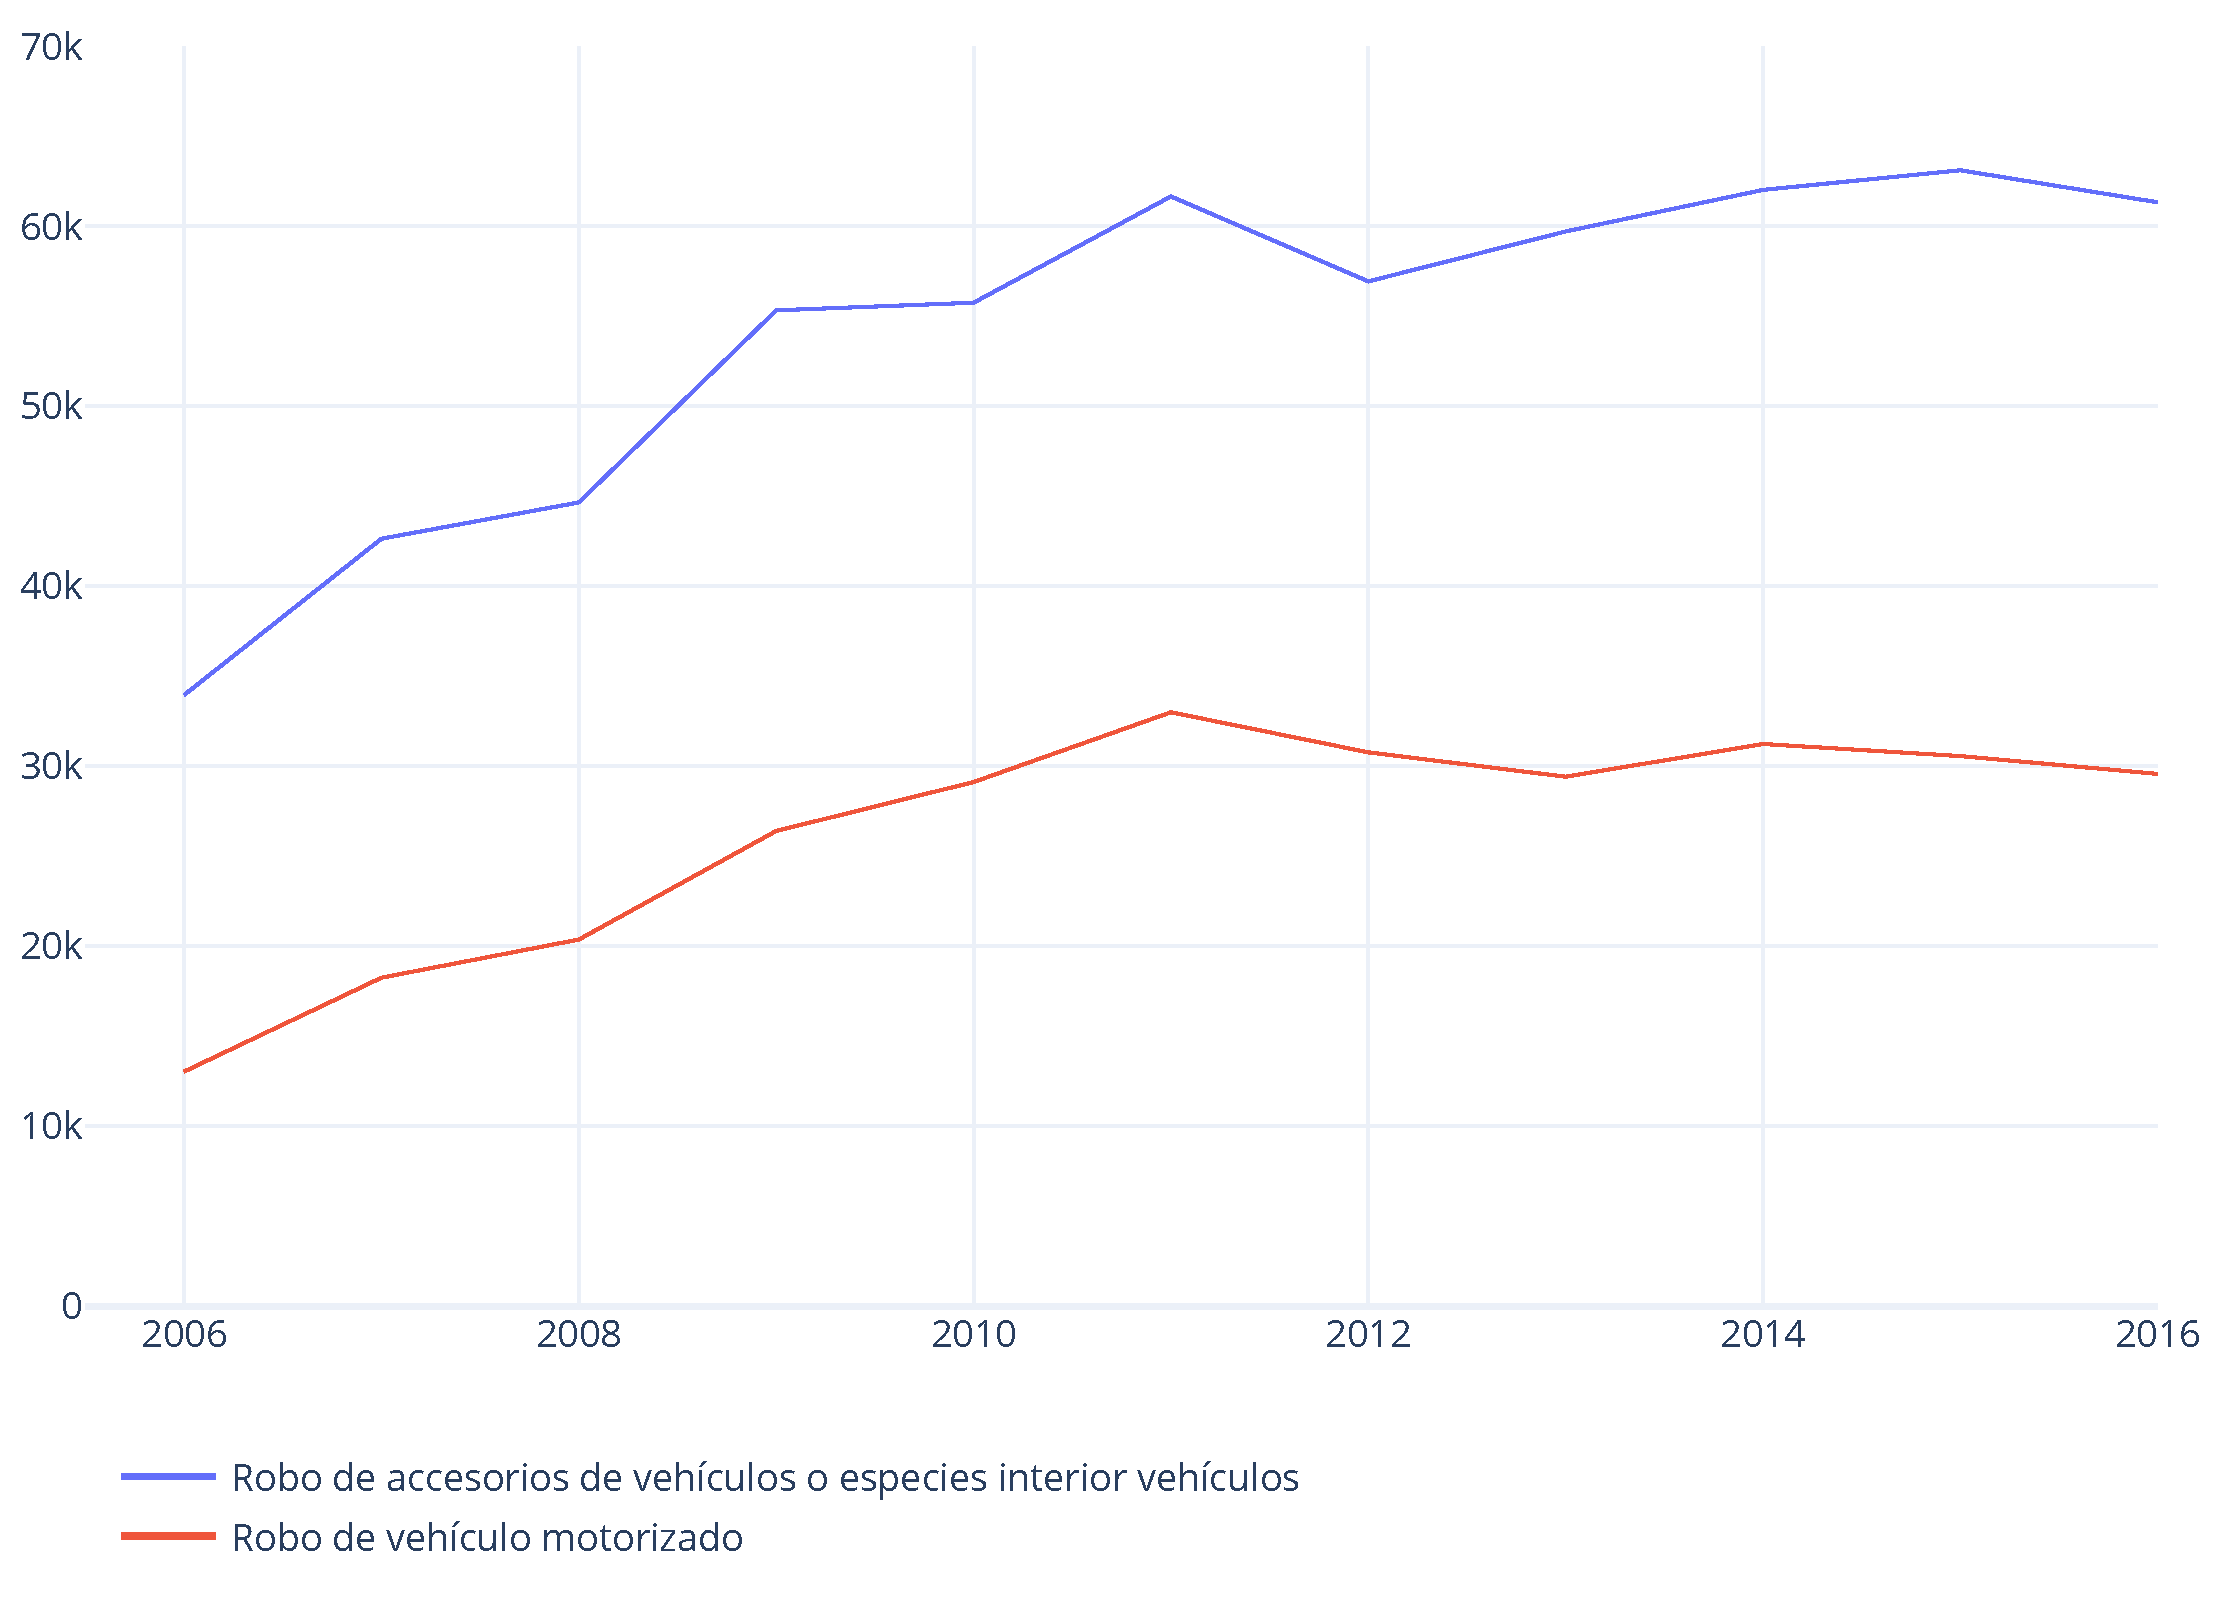
\includegraphics[width=1\textwidth]{ch1/robberies.eps} 
    \caption{Cantidad de robos de vehículos y accesorios anuales en Chile entre los años 2006-2016. Fuente: Informe anual de Carabineros, 2006-2016, INE.} 
    \label{fig:antecedente}
\end{figure}

Este fenómeno trae consigo un montón de costos para la sociedad, como incremento en la percepción de la seguridad, aumentos en la prima de los seguros de los asegurados, aumento en los costos de las aseguradoras \footnote{Considerando que el costo promedio incurrido en un auto asegurado robado y no recuperado es de \$ 5,000,000 de pesos, la pérdida total considerando solo los vehículos no recuperados para el año 2015 es de unos \$15,720 millones de pesos.} y el incremento de otros tipos de delitos. \footnote{El destino de los vehículos robados es variado, se usan los autos para perpetrar otros delitos y huir, venderlos por piezas en talleres clandestinos o blanquear sus documentos para pasarlos por la frontera y venderlos o cambiarlos por otros bienes en el extranjero.}\\

El corpus utilizado correspode a una colección de 49,015 relatos de víctimas de robo de vehículo, entre los años 2011-2016, provistos por la Asociación de Aseguradores de Chile (AACH). Cabe destacar que se estima que un tercio del parque automotriz se encuentra asegurado\footnote{\href{http://www.economiaynegocios.cl/noticias/noticias.asp?id=185224}{http://www.economiaynegocios.cl/noticias/noticias.asp?id=185224}}, por lo que se trabaja con una muestra del parque automotriz.\\

En el contexto de robo de vehículos, los tópicos pueden interpretarse como los \quotes{modus operandi} que utilizan los delicuentes para robar un vehículo. Así, la metodología propuesta permite descubrir los \textit{modus operandi} ocultos en los relatos de las víctimas y caracterizarlos a partir de las palabras, como también ver su evolución a través del tiempo, siendo capaz de detectar cuando nacen y mueren, y como cambian en el tiempo.\\

\section{Revisión del estado del arte}

El problema enunciado consiste en una tarea de \textit{clustering}, debido a que no se cuenta con una etiqueta del tema al que corresponde cada documento, siendo el propósito del trabajo descubrirla. El modelamiento de tópicos es uno de los enfoques más prometores de \textit{clustering} aplicado a texto, siendo su objetivo descubrir los temas (\textit{clusters}) ocultos presentes en el corpus, permitiendo resumir, organizar y explorar grandes colecciones de datos.\\

Algunas de las técnicas de modelamiento de tópicos están basadas en factorización matricial como LSI (Latent Semantic Indexing) \citep{dumais2004latent} o NMF (Non-negative Matrix Factorization)\citep{xu2003document}, pero este trabajo está basado en modelos probabilísticos generativos, como LDA (Latent Dirichlet Allocation)\citep{blei2003latent} o HDP (Hierarchical Dirichlet Process)\citep{teh2005sharing}. Ambos enfoques tienen sus pros y contras, en este trabajo se escoge el enfoque probabilístico ya que es capaz de expresar incertidumbre en la asignación de un tópico a un documento y en la asignación de palabras a los tópicos, además, este enfoque suele aprender tópicos más descriptivos \citep{stevens2012exploring}.\\

En el modelamiento de tópicos se pueden presentar los siguientes dinamismos:
\begin{enumerate}
    \item \textbf{Evolución de los tópicos}: la evolución de los tópicos se refleja en el cambio en la distribución sobre las palabras. Por ejemplo, el \quotes{portonazo} en un determinado momento se comete en grupos de 2-3 personas con arma blanca, luego evoluciona de arma blanca a arma de fuego y lo perpetran jóvenes menores de edad.
    \item \textbf{Dinámismo en la mezcla de tópicos}: esto permite capturar la popularidad de los tópicos en el tiempo.
    \item \textbf{Nacimiento, muerte, fusión y división de tópicos}: En el contexto de robos es natural que en el tiempo aparezcan nuevos \textit{modus operandi} como también que desaparezcan aquellos que ya no parecen tan atractivos.
\end{enumerate}

En el modelamiento de tópicos estático destaca LDA y HDP. La diferencia principal es que LDA necesita de antemano fijar el número de tópicos a descubrir y HDP lo infiere a partir del corpus.\\

Dentro de los primeros modelos de tópicos dinámicos exitosos está Dynamic Topic Modelling (DTM) junto Topic Over Time (TOC)\citep{wang2006topics}. Estos modelos mantienen el número de tópicos fijo en el tiempo, por lo que si aparece un nuevo tópico este quedará clasificado dentro de un tópico preexistente desde el comienzo, por lo que solo es capaz de capturar el punto 1 y 2.\\

En \citep{ahmed2012timeline} se propone Dynamic Hierarchical Dirichlet Process (DHDP), modelo que no mantiene el número de tópicos fijo en el tiempo, sino que lo infiere a partir del corpus. Sin embargo, este modelo no es capaz de capturar fusión y división de tópicos. Además, a diferencia de los otros modelos de tópicos mencionados, DHDP no es una tecnología ampliamente usada y no cuenta con una implementación disponible, por lo que se desconoce su desempeño en otras fuentes de información.\\

En \citep{wilson2011tracking} y \citep{beykikhoshk2018discovering} se propone una metodología que permite capturar los dinámismos mencionados utilizando LDA y HDP respectivamente. Estas consisten en dividir el corpus en épocas, entrenar de forma independiente un modelo de tópico en cada época, para finalmente unir los resultados obtenidos. En este trabajo se utilizan técnicas de modelado dinámico de tópicos bajo este enfoque, usando HDP para el descubirmiento de tópicos en cada época.

\section{Estructura de la tesis}
En el capítulo \ref{ch:theorethical_framework} se describen los fundamentos teóricos en los que se basa la metodología propuesta la cual es descrita en el capítulo \ref{ch:methodology}. Luego, en el capítulo \ref{ch:case_study} se presenta un análisis cuantitativo y cualitativo de la metodología propuesta en el fenómeno de robo de vehículos. Finalmente, en el capítulo \ref{ch:conclusion} se presentan las conclusiones y futuras lineas de investigación.


\chapter{Marco teórico}
\label{ch:theorethical_framework}
En este capítulo se describen los conceptos fundamentales para comprender la metodología propuesta en el capitulo \ref{ch:methodology}. El capítulo es estructurado como sigue. En la sección \ref{sec:mixture_models} se introduce a nivel general los modelos de \textit{clustering} probabiĺísticos conocidos como \textit{mixture models}. En la sección \ref{sec:topic_models} se describen los modelos de tópicos estáticos LDA y HDP. Finalmente, en la sección \ref{sec:topic_evolution} se explica una metodología que modela la evolución de los tópicos en el timepo. 

\section{Mixture Models}
\label{sec:mixture_models}

Uno de los supuestos básicos en \textit{clustering} es asumir que cada observación $x_{i}$ pertenece a un solo \textit{cluster} $k$. Podemos expresar la asignación a un \textit{cluster} como una variable aleatoria $z_{i}$, donde $z_{i}=k$ significa que $x_{i}$ pertenece al \textit{cluster} $k$. La variable $z_{i}$ no es observada en los datos y se considera una variable oculta. Cada \textit{cluster} posee un parámetro $\phi_{k}$ que codifica su información. Podemos obtener la distribución que caracteriza a un solo \textit{cluster} $k$ condicionando en $z_{i}$

\begin{align}
    p(x_{i}|z_{i}=k, \phi) = p(x_{i}|\phi_{k})\\
\end{align}

Además, podemos definir la probabilidad de que una nueva observación pertenezca al \textit{cluster} $k$ 

\begin{align}
    p(z_{i}=k|\pi) = \pi_{k}
\end{align}

Con $\sum_{k}\pi_{k} = 1$, ya que $\pi_{k}$ son probabilidades de eventos mutuamente excluyentes. La distribución de $x_{i}$ es entonces de la forma

\begin{align}
  p(x_{i}) = \sum_{k}p(z_{i}=k|\pi)p(x_{i}|z_{i}=k, \phi) = \sum_{k}\pi_{k}p(x_{i}|\phi_{k})
\end{align}

Podemos escribir $p(x_{i}|\phi_{k})$ como $x_{i} \sim F(\phi_{z_{i}})$, donde $F$ es la distribución asociada a las observaciones. \\

Se obtiene una representación equivalente del modelo al considerar el parámetro $\phi_{z_{i}}$ usado para generar la observación $x_{i}$ proviene de una distribucion discreta $G$, la cual tiene la forma

\begin{align}
    G(\phi) & = \sum_{k} \pi_{k}\delta_{\phi_{k}}(\phi)
\end{align}

En otras palabras, $G$ es una mezcla de funciones delta, donde la probabilidad de que $\phi$ sea igual a $\phi_{k}$ es $\pi_{k}$. Luego, un \textit{mixture model} se puede  representar como a continuación

\begin{align}
\phi_{z_{i}} & \sim G\\
x_{i} & \sim  F(\phi_{z_{i}})
\end{align}

Un \textbf{Bayesian mixture model} es un \textit{mixture model} con una medida aleatoria para las mezclas. En la sección \ref{sec:dirichlet}. y \ref{sec:dp} nos referimos a dos \textit{priors} ampliamente usados para construir \textit{bayesian mixture model}: la distribución Dirichlet que nos permite construir un \textbf{finite mixture model}, donde el número de átomos o \textit{clusters} a descubrir es finito, denotado por $K$ y un \textit{prior} no paramétrico denominado Dirichlet Process (DP), el cual permite construir un \textbf{infinite mixture model}, donde el número de \textit{clusters} no está acotado. 

\subsection{Distribución Dirichlet}
\label{sec:dirichlet}

La distribución Dirichlet \citep{minka2000estimating} es una generalización multivariada de la distribución beta, la cual tiene soporte sobre un \textbf{simplex}, definido por:
\begin{equation}
    S_{K} = \big\{x: 0\leq x_{k} \leq 1, \sum_{k=1}^{K}x_{k}=1\big\}
\end{equation}
Luego, su función de densidad de probabilidad (pdf):

\begin{equation}
    Dir(x|\alpha)=\frac{1}{B(\alpha)}\prod_{k=1}^{K}x_{k}^{\alpha_{k}-1}\mathbb{I}(x\in S_{K})
\end{equation}

, donde $B(\alpha) = B(\alpha_{1}, \ldots, \alpha_{K})$ es la generalización de la función beta a $K$ variables:

\begin{align}
    B(\alpha) \triangleq \frac{\prod_{k=1}^{K}\Gamma(\alpha_{k})}{\Gamma(\alpha_{0})}
\end{align}

, donde $\alpha_{0} \triangleq \sum_{k=1}^{K}\alpha_{k}$.\\

En la Figura \ref{img:dirichlet_distribution} se observa el efecto de los parámetros en la distribución Dirichlet con $K=3$. El parámetro $\alpha_{k}$ controla la \textit{sparsity}, mientras más se acerca a 0 los vectores generados tienen más átomos nulos y se concentra la masa en unas pocas coordenadas, mientras más grande $\alpha_{k}$ la masa más se concentra en el centro (1/3, 1/3, 1/3). Cuando $\alpha_{k}=1$ se tiene una distribución uniforme en el dominio $S_{K}$. Por otro lado, cuando $\alpha$ no es simétrico la masa se concentra proporcionalmente en las coordenadas con $\alpha_{k}$ mayor.\\

\begin{figure}
    \centering
    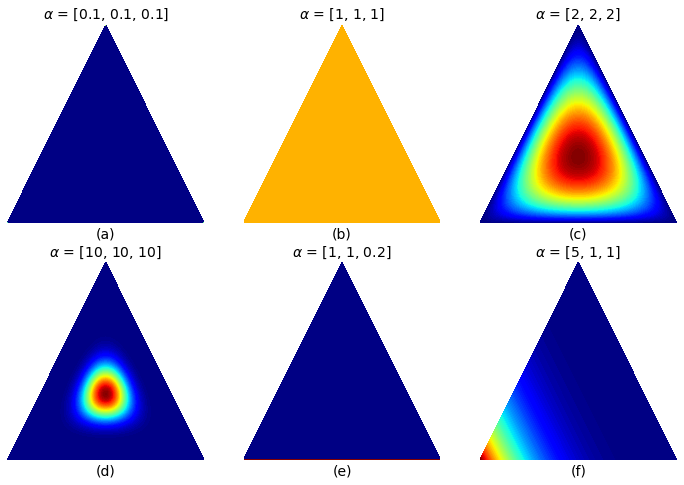
\includegraphics[width=\textwidth]{ch2/dirichlet_simplex.eps}
    \caption{Densidad de la distribución Dirichlet con $K=3$. Define una distribución sobre el \textit{simplex}, el cual puede ser representado por una superficie trinagular.}
    \label{img:dirichlet_distribution}
\end{figure}

En general se asume simetría en los parámetros de la distribución Dirichlet de la forma $\alpha_{k}=\frac{\alpha}{K}$, de esta manera $\alpha$ funciona como parámetro de concentración. En la Figura \ref{img:dirichlet_samples} se oberva una realización de una distribución Dirichlet con $\alpha \in \{0.1, 1, 10\}$ y $K\in\{2, 10, 100\}$. En esta figura podemos observar que a mayor $\alpha$ los compenentes del vector $x$ más similares se vuelven, esto es más notorio a mayor dimencionalidad debido a que existen más dimensiones a las que distribuir la masa.\\

La distribución Dirichlet es comúnmente usada en estadística Bayesiana, debido a que que es \textit{prior} conjugado de la distribución categórica (multinoulli) y la distribución multinomial. Así, la distribución Dirichlet puede ser utilizado como \textit{prior} en un \textit{finite mixture model} considerando $\pi\sim \text{Dir}(\frac{\alpha}{K}1_{K})$ y $\phi_{k} \sim H$.

\begin{figure}
    \centering
    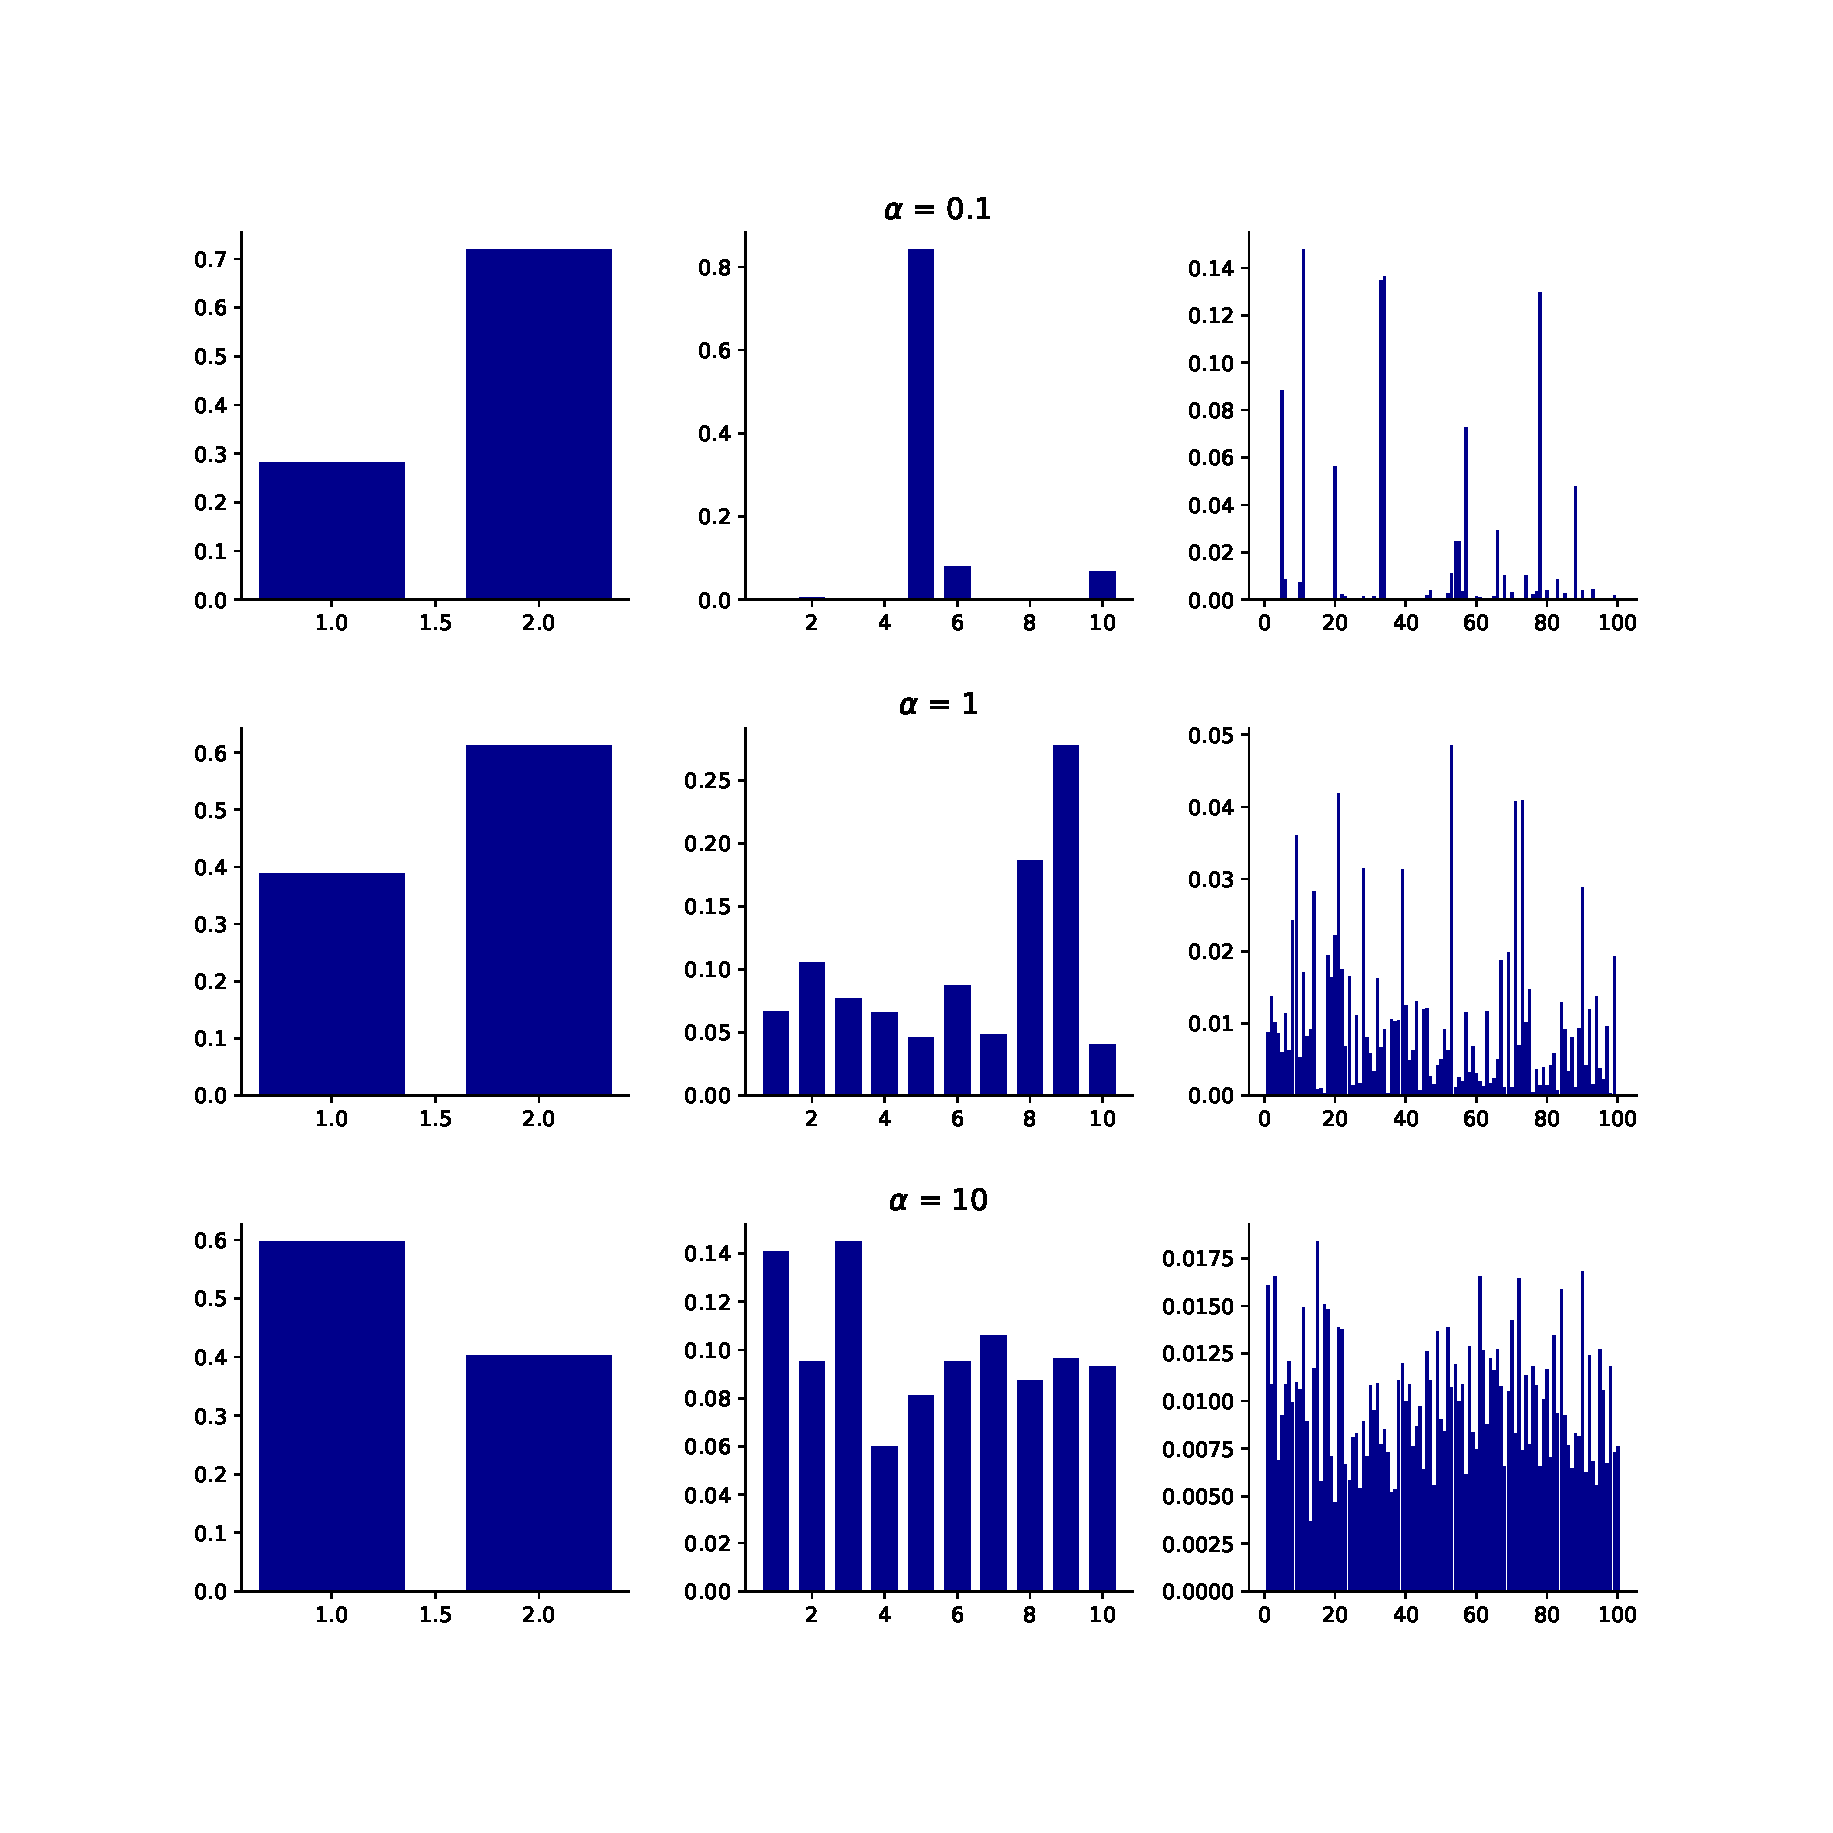
\includegraphics[width=\textwidth]{ch2/dirichlet_samples.eps}
    \caption{Muestra de una distribución Dirichlet simétrica con $\alpha \in \{0.1, 1, 10\}$ y $K\in\{2, 10, 100\}$.}
    \label{img:dirichlet_samples}
\end{figure}

\subsection{Dirichlet Process}
\label{sec:dp}

En un \textit{finite mixture model} se tiene $G(\phi) = \sum_{k=1}^{K} \pi_{k}\delta_{\phi_{k}}(\phi)$, luego al muestrear de $G$, con probabilidad uno se obtendrá exactamente $K$ \textit{clusters}. Nos gustaría tener un modelo más flexible, que pueda generar un número variable de \textit{clusters}. Una forma de hacer esto es remplazar la distribución discreta $G$ por una medida aleatoria de probabilidad, como el Dirichlet Process \citep{ferguson1973bayesian}, denotado $G\sim \text{DP}(\alpha, H)$.\\

Un \textbf{Dirichlet Process} (DP) es una distribución sobre medidas de probabilidad $G: \Phi \rightarrow \mathbb{R}^{+}$, donde $G(\phi)\geq 0$ y $\int_{\Phi}G(\phi)d\phi=1$. Un DP se define implícitamente por cumplir 

\begin{align}
    G(A_{1}), \ldots, G(A_{K}) \sim \text{Dir}(\alpha H(A_{1}), \ldots, \alpha H(A_{K}))
\end{align}

para cualquier partición finita $(A_{1}, \ldots, A_{k})$ de $\Phi$. En este caso, decimos que $G\sim \text{DP}(\alpha, H)$, donde $\alpha$ es llamado el \textbf{parámetro de concentración} y $H: \Phi \rightarrow \mathbb{R}^{+}$ es llamado la \textbf{medida base}.\\

Como $p(G(A_{1}), \ldots, G(A_{K}))$ es Dirichlet, la distribución marginal en cada partición distribuye beta $\text{Beta}(\alpha H(A_{i}), \alpha \sum_{j\neq i}H(A_{j}))$. El DP es considerado consistentemente definido, en el sentido de que si particionamos $\bar{A}_{1}$ en $A_{1}$ y $A_{2}$, entonces $G(\bar{A}_{1})$ y $G(A_{1})+G(A_{2})$ siguen la misma distribución beta. \\

Sea $\phi \sim \text{Dir}(\alpha)$, y $z|\phi  \sim \text{Cat}(\pi)$, si se integra $\pi$ afuera se obtiene la distribución predictiva del modelo Dirichlet-multinoulli:
\begin{align}
    z\sim \text{Cat}(\alpha_{1}/\alpha_{0}, \ldots, \alpha_{K}/\alpha_{0})
\end{align}
donde $\alpha_{0} = \sum_{k}\alpha_{k}$. Es decir, $p(z=k|\alpha)=\alpha_{k}/\alpha_{0}$. Ademas, la posterior de $\pi$ dada una observación viene dada por
\begin{align}
    \pi|z \sim \text{Dir}(\alpha_{1}+\mathbb{I}(z=1), \ldots, \alpha_{K}+\mathbb{I}(z=K))
\end{align}

El DP generaliza el resultado anterior a particiones arbitrarias. Si $G\sim \text{DP}(\alpha, H)$, luego $p(\phi \in A_{i})=H(A_{i})$ y la posterior es

\begin{align}
    p(G(A_{1}), \ldots, G(A_{K})|\phi, \alpha, H) = \text{Dir}(\alpha H(A_{1})+\mathbb{I}(\phi \in A_{1}), \ldots, \alpha H(A_{K})+\mathbb{I}(\phi \in A_{K}))
\end{align}

Esto se mantiene para cualquier conjunto de particiones. Por lo tanto, si observamos multiples muestras $\bar{\phi}_{1:N}\sim G$, la nueva posterior está dada por 

\begin{align}
G|\bar{\phi}_{1:N}, \alpha, H \sim \text{DP}\bigg(\alpha+N, \frac{1}{\alpha+N}\bigg(\alpha H+\sum_{i=1}^{N}\delta_{\phi_{i}}\bigg)\bigg)
\end{align}

Por ende el DP define un \textit{prior} conjugado para cualquier espacio medible, donde el parámetro de concentración $\alpha$ es el tamaño de muestro efectivo de la medida base $H$.\\

Existen diferentes perspectivas que ayudan a entender la propiedad de \textit{clustering} de un Dirichlet Process. En la sección \ref{sec:sbp}. y \ref{sec:crp}. se describen dos: el Stick Breaking Process y Chinese Restaurant Process (CRP).

\subsection{Stick Breaking Process}
\label{sec:sbp}

En esta sección se describe una definición constructiva de un DP, conocida como \textit{stick breaking process} \citep{sethuraman1994constructive}. Sea $\pi=\{\pi_{k}\}_{k=1}^{\infty}$ una mezcla de pesos infinita derivada a partir del siguiente proceso:
\begin{align}
    \beta_{k} & \sim \text{Beta}(1, \alpha)\\
    \pi_{k} & = \beta_{k}\prod_{l=1}^{k-1}(1-\beta_{l}) = \beta_{k}(1-\sum_{l=1}^{k-1}\pi_{l})
\end{align}

Esto se suele denotar como $\pi \sim \text{GEM}(\alpha)$, donde GEM representa Griffiths, Engen y McCloskey, ver Figura  \ref{img:stick_breaking} para una ilustración. 

\begin{figure}
    \centering
    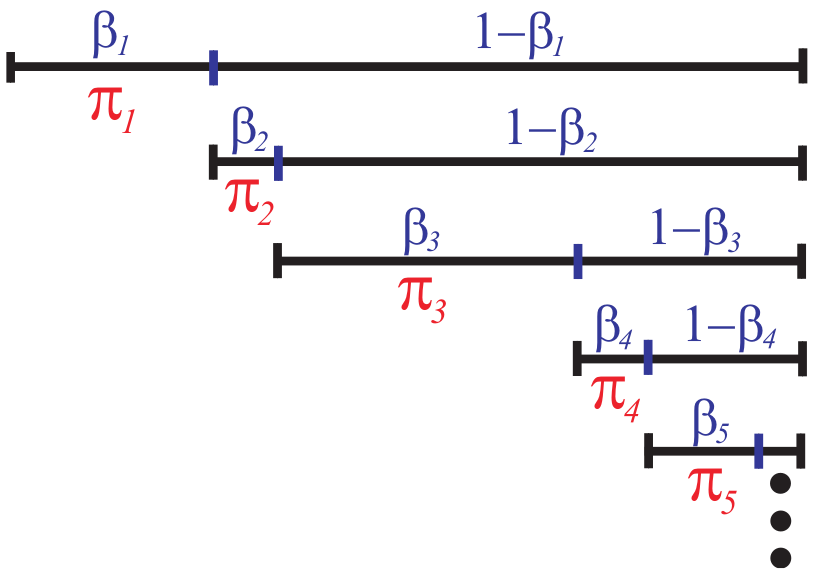
\includegraphics[width=0.6\textwidth]{ch2/stick_breaking.png}
    \caption{Ilustración de \textit{stick breaking process}. Se tiene una barra de largo 1, la cual se rompe en un punto aleatorio $\beta_{1}$, el largo de la pieza restante es llamada $\pi_{1}$, luego recursivamente se rompe la barra restante, así generando $\pi_{2}, \pi_{3}, \ldots$. Fuente: Figura 2.22 de \citep{sudderth2006graphical}.}
    \label{img:stick_breaking}
\end{figure}

Algunos ejemplos de este proceso son mostrados en la Figura \ref{img:dp_samples} (a). A mayor $\alpha$, menos varianza y mayor número de átomos, por el contrario, pequeños valores de $\alpha$ muestran una alta varianza y menor número de átomos. Se puede demostrar que este proceso terminará con probabilidad uno, a pesar que el número de elementos que genera incrementa con $\alpha$. Además, el tamaño del componente $\pi_{k}$ decrece en promedio. La distribución $G$ se puede definir como sigue:

\begin{align}
    G(\phi) = \sum_{k=1}^{\infty}\pi_{k}\delta_{\phi_{k}}(\phi)
\end{align}
 
, donde $\pi \sim \text{GEM}(\alpha)$ y $\phi_{k} \sim H$. Es posible demostrar que $G \sim \text{DP}(\alpha, H)$. Como consecuencia de esta construcción, las muestras de un DP son \textbf{discretas con probabilidad uno}. En otras palabras, al muestrear $\bar{\phi_{i}}\sim G$ se observarán valores repetidos, por lo que la mayoría de los datos vendrán de los $\phi_{k}$ con $\pi_{k}$ más largos. En la Figura \ref{img:dp_samples} (b) se muestra un par de medidas aleatorias generadas a partir de un DP con una medida base normal.\\

\begin{figure}
    \centering
    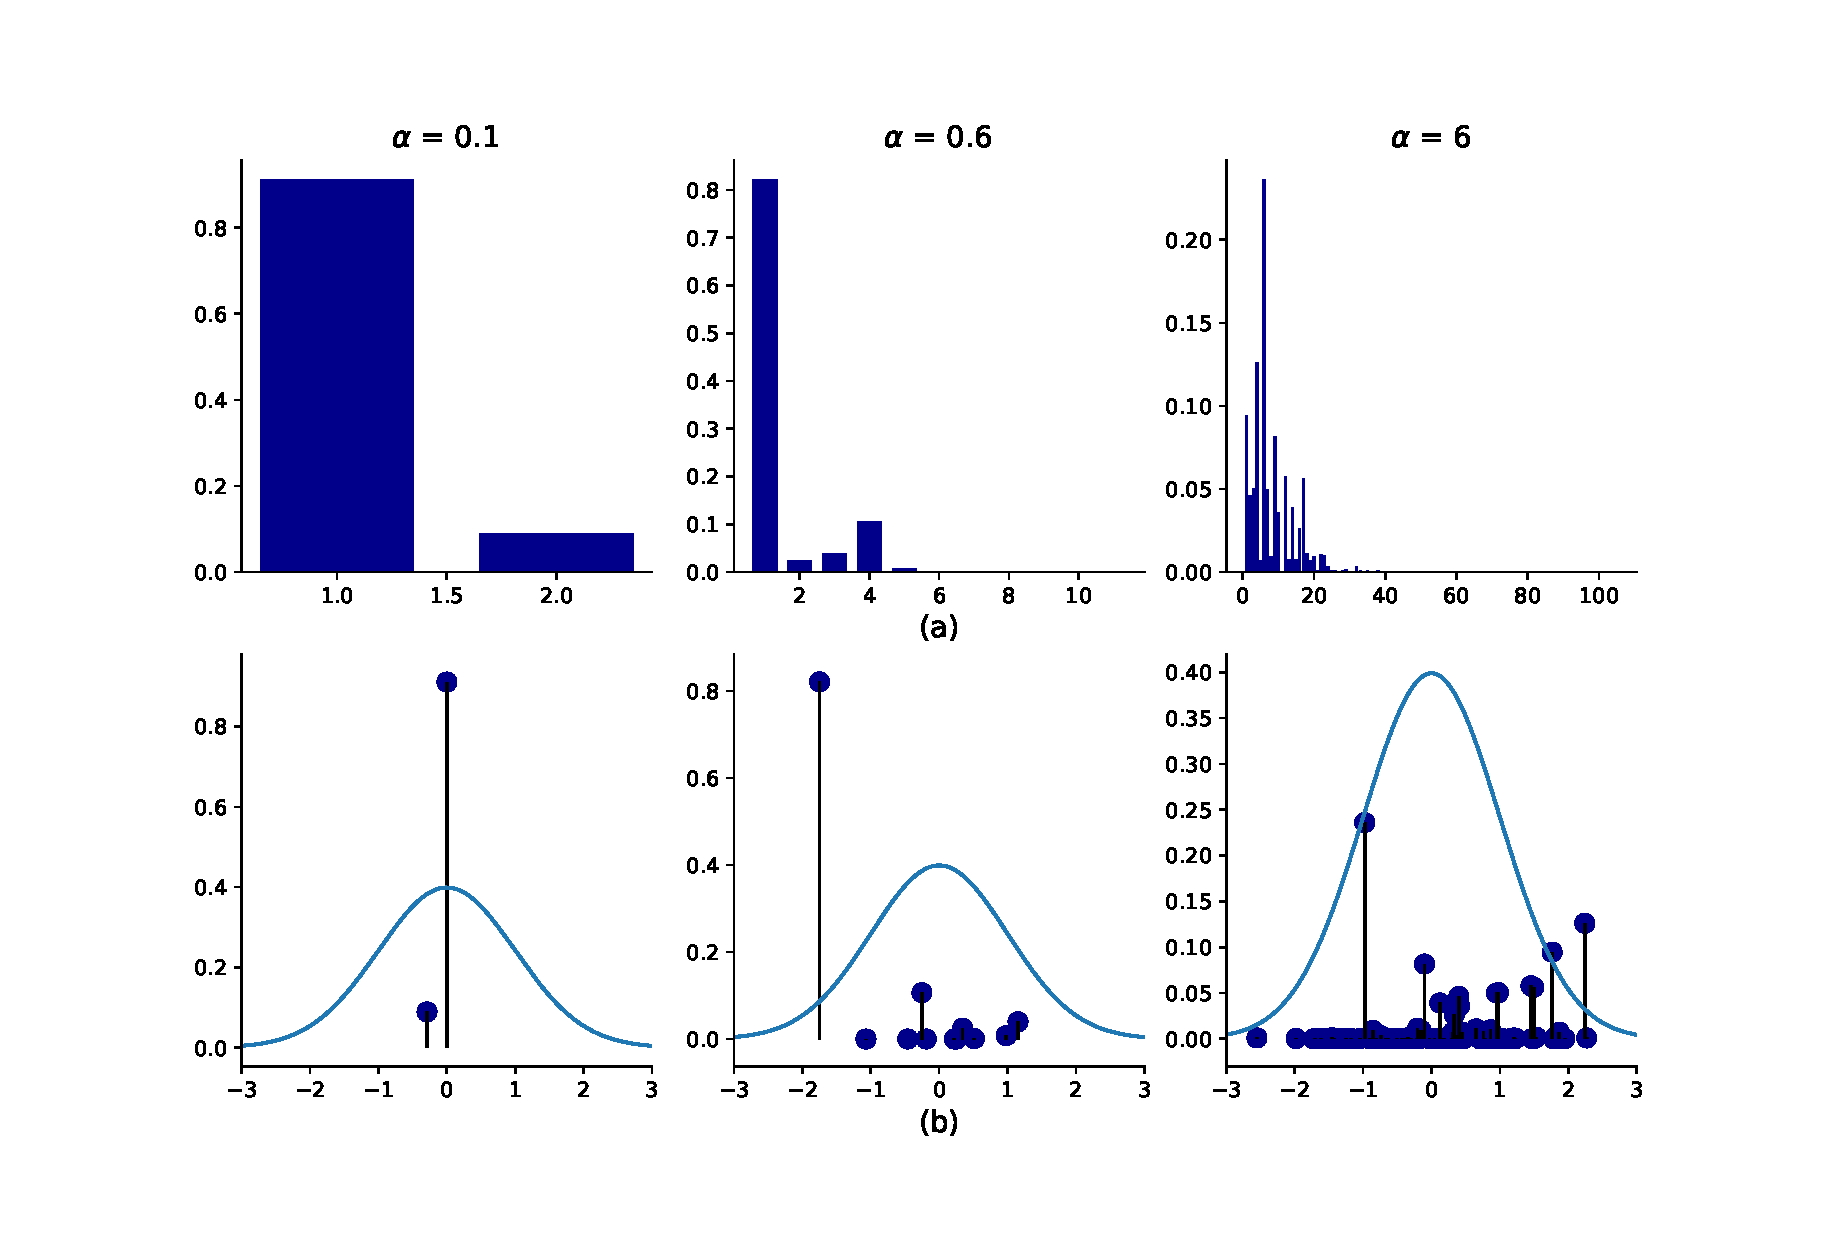
\includegraphics[width=\textwidth]{ch2/dp_samples.eps}
    \caption{(a) Muestras de una distribución GEM con parámetros de concentración $\alpha\in \{0.1, 0.6, 6\}$. (b) Medidas aleatorias generadas a partir de un Dirichlet Process con medida base normal $\mathcal{N}(0,1)$ con parámetros de concentración $\alpha\in \{0.1, 0.6, 6\}$}
    \label{img:dp_samples}
\end{figure}

\subsection{Chinese Restaurant Process}
\label{sec:crp}

Trabajar con infinitos átomos puede ser bastante problemático. Para sortear esta dificultad se puede explotar la propiedad de \textit{clustering} de un DP. Sea $\bar{\phi}_{1:N}\sim G$ observaciones generadas a partir de $G\sim \text{DP}(\alpha, H)$, sea $K$ los distintos valores de $\bar{\phi}_{1:N}$, luego la distribución predictiva condicionada en las $N$ observaciones está dada por

\begin{align}
p(\bar{\phi}_{N+1}=\phi|\bar{\phi}_{1:N}, \alpha, H) = \frac{1}{\alpha+N}\bigg(\alpha H(\phi)+\sum_{k=1}^{K}N_{k}\delta_{\bar{\phi}_{k}}(\phi)\bigg)
\end{align}

donde $N_{k}$ es el número de observaciones previas iguales a $\phi_{k}$. Este esquema de muestreo es llamado \textit{Polya urn} o \textit{Blackwell-MacQueen}. \\

Es más conveniente trabajar con variables discretas $z_{i}$ que especifican cual $\phi_{k}$ usar, así, se define $\bar{\phi}_{i}=\phi_{z_{i}}$. En base a esta expresión se tiene lo siguiente:

\begin{align}
p(z_{N+1}=z|z_{1:N}, \alpha) = \frac{1}{\alpha+N}\bigg(\alpha\mathbb{I}(z=k^{*})+\sum_{k=1}^{K}N_{k}\mathbb{I}(z=k)\bigg)
\end{align}

, donde $k^{*}$ representa un nuevo \textit{cluster} que no ha sido usado aún. Este proceso es denominado Chinese Restaurant Process (CRP) \citep{aldous1985exchangeability}, basado en la oferta aparentemente infinita de mesas en ciertos restaurantes Chinos. La analogía es la siguiente: Las tablas del restaurante son los \textit{clusters}  y los clientes son las observaciones. Cuando una persona entra al restaurante, esta puede escoger sentarse en una tabla existente con probabilidad proporcional al número de personas ya sentadas en esa tabla ($N_{k}$), en otro caso, con una probabilidad decreciente a medida que más personas entran al restaurante (debido a $1/(\alpha +N))$ escogerá sentarse en una nueva tabla $k^{*}$. El resultado de este proceso es una distribución sobre particiones de los naturales, la cual es como una distribución de clientes a tablas.\\

El hecho de que las tablas actualmente ocupadas son más probables de obtener nuevos clientes se suele llamar el fenómeno del \textit{rich get richer}. En efecto, se puede demostrar que la dsitribución del número de \textit{clusters} que induce este \textit{prior} es básicamente una ley de potencia, donde el número de tablas $K$ con probabilidad 1 se aproxima a $\alpha log(N)$ cuando $N\rightarrow \infty$, mostrando que la complejidad del modelo crece logarítmicamente con el tamaño de los datos.

\section{Modelos de tópicos}
\label{sec:topic_models}
Los modelos de tópicos probabilísticos ayudan a descubrir los temas latentes (\textit{clusters}) en una colección de documentos, como estos temas están conectados unos a otros y cómo cambian en el tiempo. Permiten resumir un gran colección de documentos a través de sus temas y organizarlos entorno a estos.\\

Los modelos probabilísticos tratan un tópico como una distribución de probabilidad discreta sobre el vocabulario del corpus, siendo un práctica habitual interpretar un tópico a partir de sus $N$ palabras más probables. Por ejemplo, con $N=5$ las palabras más probables de un tópico son: \quotes{llaves}, \quotes{domicilio}, \quotes{individuos}, \quotes{casa} y \quotes{porton}, por lo que una etiqueta valida para este tópico podría ser \quotes{portonazo}.\\ 

En \textit{procesamiento del lenguaje natural} (NLP) se suele trabajar bajo la asumpción de \textbf{bag of words} (bolsa de palabras), es decir, tanto los documentos como las palabras son tratadas como intercambiables. Es importante hacer notar que itercambiabilidad no es equivalente a que las variables aleatorias son independientes e identicamente distribuidas. Más bien, intercambiabilidad esencialmente puede ser interpretado como condicionalmente independientes e identicamente distribuidas, donde el condicionamiento es con respecto a los parámetros de una distribución de probabilidad. Por lo tanto, el supuesto de intercambiabilidad es claramente un supuesto de simplificación cuya principal justificación es la construcción de algoritmos computacionales más eficientes.\\

Un \textit{mixture model} que trabaja bajo la asumpción de \textit{bag of words} es \textit{mixture of unigrams} \citep{nigam2000text}, el cual asume que todos los documentos provienen de un solo \textit{cluster} dentro de un conjunto finito de $K$ \textit{clusters}. Los documentos de un \textit{cluster} discuten solo un tópico particular $z$, y cada tópico $z$ está asociado a una distribución categórica. Así, la verosimilitud de observar un documento $d$ es

\begin{align}
    w|z &\sim \text{Cat}(\theta_{z})\\
    p(w_{1}, \ldots, w_{N_{d}}) &= \sum_{z=1}^{K}p(z)\prod_{i=1}^{N_{d}}p(w_{i}|z)
\end{align}

En las secciones \ref{sec:lda}-\ref{sec:hdp} se describe en detalle dos modelos de tópicos probabilísticos, Latent Dirichlet Allocation (LDA) y Hierarchical Dirichlet Process (HDP), considerado la generalización no parámetrica de LDA, donde el número de tópicos a descubrir no está acotado y se infiere a partir del corpus.\\

En comparación a \textit{mixture of unigrams}, LDA y HDP suponen que las palabras de un documento provienen de un mismo \textit{mixture model}, donde a nivel corpus los \textit{mixture models} comparten parámetros, que vienen siendo los tópicos, pero las \textit{mixtures of topics} son específicas de cada documento. Esto permite relajar la asumpción de que cada documento es generado por un solo tópico, debido a que cada palabra proviene de algún tópico, por lo que un documento puede tener presencia de más de un tema.\\

\subsection{Latent Dirichlet Allocation}
\label{sec:lda}

En Latent Dirichlet Allocation (LDA) \citep{blei2003latent} cada tópico es una distribución de probabilidad sobre un vocabulario fijo $V$. Cada documento $d$ tiene su propia mezcla de tópicos $\pi_{d}$. La asignación $z_{d,n}\in\{1, \ldots, K\}$  de de una palabra $n$ a un tópico $z$ es dibujada a partir de $\pi_{d}$. El modelo completo es como sigue

\begin{align}
    \phi_{k}|\eta \quad & \sim\quad \text{Dir}(\frac{\eta}{|V|}1_{|V|})\\
    \pi_{d}|\alpha \quad & \sim \quad \text{Dir}(\frac{\alpha}{K}1_{K})\\
    z_{d,n}|\pi_{d} \quad & \sim \quad \text{Cat}(\pi_{d})\\
    w_{d,n}|z_{d,n}, \phi_{1:K} \quad & \sim \quad \text{Cat}(\phi_{z_{d,n}})
\end{align}

Esto es ilustrado en la Figura \ref{img:lda}.
\begin{figure}
  \centering
  \tikz{ %

    \node[latent, dashed] (alpha) {$\alpha$} ; %
    \node[latent, right=of alpha] (pi) {$\pi_{d}$} ; %
    \node[latent, right=of pi] (z) {$z_{d,n}$} ; %
    \node[obs, right=of z] (w) {$w_{d,n}$}   ; %
    \node[latent, right=of w] (phi) {$\phi_{k}$} ; %
    \node[latent, right=of phi, dashed] (eta) {$\eta$} ;%
    \plate[inner sep=0.25cm, xshift=-0.12cm, yshift=0.12cm] {plate1} {(z) (w)} {$N_{d}$}; %
    \plate[inner sep=0.25cm, xshift=-0.12cm, yshift=0.12cm] {plate2} {(pi) (plate1)} {$D$}; %
    \plate[inner sep=0.25cm, xshift=-0.12cm, yshift=0.12cm] {plate3} {(phi)} {$K$}; %
    \edge {alpha} {pi} ; %
    \edge {pi} {z} ; %
    \edge {z,phi} {w} ; %
    \edge {eta} {phi} ; %
  }
\caption{Representación gráfica de LDA: círculos denotan variables aleatorias, círculos abiertos denotan parámetros, círculos sombreados denotan variables observadas y los platos indican replicación.}
\label{img:lda}
\end{figure}

La probabilidad conjunta del modelo:
\begin{equation}
    p(\phi, \pi, z, w|\alpha, \eta)= \prod_{k=1}^{K}p(\phi_{k}|\eta)\prod_{d=1}^{D}p(\pi_{d}|\alpha)\prod_{n=1}^{N_{d}}p(z_{n,d}|\pi_{d})p(w_{d,n}|\phi_{1:K}, z_{d,n})
\end{equation}

La distribución a posterior:
\begin{equation}
    p(\phi, \pi, z|w, \alpha, \eta) = \frac{p(\phi, \pi, z, w|\alpha, \eta)}{p(w|\alpha, \eta)}
\end{equation}

La distribución posterior es computacionalmente intratable para inferencia exacta, debido a que para normalizar la distribución se debe marginalizar sobre todas las variables ocultas y escribir la constante de normalización en términos de los parámetros del modelo. Para poder computar la posterior es necesario utilizar algoritmos de inferencia aproximada, donde el enfoque habitual es Markov Chain Monte Carlo (MCMC) \citep{andrieu2003introduction} e Inferencia Variacional (VI) \citep{blei2017variational}. En \citep{blei2003latent} se propone un algoritmo basado en VI y en \citep{griffiths2004finding} en MCMC.\\

Una representación equivalente en LDA sería generar cada palabra de un documento $d$ a partir de un tópico dibujado por una distribución $G_{d}$,

\begin{align}
    \phi_{k}|\eta \quad & \sim \quad \text{Dir}(\frac{\eta}{|V|}1_{|V|})\\
    \pi_{d}|\alpha \quad & \sim \quad \text{Dir}(\frac{\alpha}{K}1_{K})\\
    G_{d}(\phi)\quad & = \quad \sum_{k=1}^{K}\pi_{d, k}\delta_{\phi_{k}}(\phi)\\
    \phi_{d,n}|\pi_{d}, \phi_{1:K} \quad & \sim \quad G_{d}\\
    w_{d,n}|\phi_{d,n} \quad & \sim \quad  \text{Cat}(\phi_{d,n})
\end{align}

\subsection{Hierarchical Dirichlet Process}
\label{sec:hdp}

Hierarchical Dirichlet Process (HDP)\citep{teh2005sharing} es un \textit{prior} jerárquico no paramétrico, el cual está formado por un DP cuya medida base $G_{0}$ es dibujada a partir de un DP. En el caso de modelamiento de tópicos, se tiene un medida global $G_{0}$ a nivel corpus que es dibujada a partir de un DP con medida base Dirichlet y una medida para cada documento que es dibujada a partir de un DP cuya medida base es $G_{0}$. El modelo completo es como sigue

\begin{align}
   H \quad &= \quad \text{Dir}(\frac{\eta}{|V|}1_{|V|})\\
   G_{0}|\gamma, H \quad &\sim \quad \text{DP}(\gamma, H)\\
   G_{d}|\alpha, G_{0} \quad &\sim \quad \text{DP}(\alpha_{0}, G_{0})\\
   \phi_{d,n}|G_{d} \quad &\sim \quad G_{d}\\
   w_{d,n}|\phi_{d,n} \quad &\sim \quad \text{Cat}(\phi_{d,n})
\end{align}

Esto es ilustrado en la Figura \ref{img:hdp}.

\begin{figure}
  \centering
  \tikz{ %
    \node[latent, dashed] (H) {$H$} ; %
    \node[latent, right=of H] (G0) {$G_{0}$} ; %
    \node[latent, above= of G0, dashed] (gamma) {$\gamma$} ; %
    \node[latent, right=of G0] (Gd) {$G_{d}$} ; %
    \node[latent, above= of Gd, dashed] (alpha0) {$\alpha_{0}$} ; %
    \node[latent, right= of Gd] (phi) {$\phi_{d,n}$} ; %
    \node[obs, right=of phi] (w) {$w_{d,n}$}   ; %
    \plate[inner sep=0.25cm, xshift=-0.12cm, yshift=0.12cm] {plate1} {(phi) (w)} {$N_{d}$}; %
    \plate[inner sep=0.25cm, xshift=-0.12cm, yshift=0.12cm] {plate2} {(Gd) (plate1)} {$D$}; %
    \edge {H, gamma} {G0} ; %
    \edge {G0, alpha0} {Gd} ; %
    \edge {Gd} {phi} ; %
    \edge {phi} {w} ; %
  }
\caption{Representación gráfica de HDP: círculos denotan variables aleatorias, círculos abiertos denotan parámetros, círculos sombreados denotan variables observadas y los platos indican replicación.}
\label{img:hdp}
\end{figure}

La discretitud a nivel corpus de $G_{0}$ asegura que todos los documentos comparten el mismo conjunto de tópicos (\textit{mixture components}). A nivel documento $G_{d}$ hereda los tópicos de $G_{0}$, pero los pesos de cada tópico (\textit{mixture proportions}) es específica del documento.\\


\subsubsection{Stick Breaking Construction}
Aplicando \textit{stick breaking construction} se tiene que para el DP dibujado a nivel corpus la siguiente representación:

\begin{align}
    \beta_{k}^{'} \quad &\sim \quad \text{Beta}(1, \gamma) \\
    \beta_{k} \quad &= \quad \beta_{k}^{'}\prod_{l=1}^{k-1}(1-\beta_{l}^{'})\\
    \phi_{k} \quad &\sim \quad H  \\
    G_{0}(\phi) \quad &= \quad \sum_{k=1}^{\infty}\beta_{k}\delta_{\phi_{k}}(\phi)
\end{align}

Así, $G_{0}$ es discreto y tiene soporte en los átomos $\phi = \{\phi\}_{k=1}^{\infty}$ con pesos $\beta=\{\beta_{k}\}_{k=1}^{\infty}$, siendo la distribución de $\beta$ escrita como $\beta \sim \text{GEM}(\gamma)$. La construcción a nivel documento de $G_{d}$ es:

\begin{align}
    \pi_{d,k}^{'} \quad &\sim \quad \text{Beta}\big(\alpha_{0}\beta_{k}, \alpha_{0}\big(1-\sum_{l=1}^{k}\beta_{l}\big)\big)\\
    \pi_{d,k} \quad &= \quad \pi_{d,k}^{'}\prod_{l=1}^{k-1}(1-\pi_{d,l}^{'})\\
    G_{d}(\phi) \quad &= \quad\sum_{k=1}^{\infty}\pi_{d,k}\delta_{\phi_{k}}(\phi)\\
    \phi_{d,n}|\pi_{d}, \phi_{1:\infty} \quad &\sim \quad G_{d}
\end{align}

Donde $\phi = \{\phi_{k}\}_{k=1}^{\infty}$ son los mismos átomos de $G_{0}$. Esto es ilustrado en la Figura \ref{img:hdp_sbc}.

%stick breaking
\begin{figure}
  \centering
  \tikz{ %
    \node[latent] (beta) {$\beta$} ; %
    \node[latent, above= of beta, dashed] (gamma) {$\gamma$} ; %
    \node[latent, right=of beta] (pi) {$\pi_{d}$} ; %
    \node[latent, above= of pi, dashed] (alpha0) {$\alpha_{0}$} ; %
    \node[latent, right= of pi] (z) {$z_{d,n}$} ; %
    \node[obs, right=of z] (w) {$w_{d,n}$}   ; %
    \node[latent, right=of w] (phi) {$\phi$} ; %
    \node[latent, above=of phi, dashed] (H) {$H$} ; %
    \plate[inner sep=0.25cm, xshift=-0.12cm, yshift=0.12cm] {plate1} {(z) (w)} {$N_{d}$}; %
    \plate[inner sep=0.25cm, xshift=-0.12cm, yshift=0.12cm] {plate2} {(pi) (plate1)} {$D$}; %
    \plate[inner sep=0.25cm, xshift=-0.12cm, yshift=0.12cm] {plate3} {(phi)} {$K (\infty)$}; %
    \edge {gamma} {beta} ; %
    \edge {beta, alpha0} {pi} ; %
    \edge {pi} {z} ; %
    \edge {z, phi} {w} ; %
    \edge {H} {phi} ; %
  }
\caption{Representación gráfica de la construcción stick-breaking de HDP: círculos denotan variables aleatorias, círculos abiertos denotan parámetros, círculos sombreados denotan variables observadas y los platos indican replicación.}
\label{img:hdp_sbc}
\end{figure}

\subsubsection{Chinese Restaurant Franchise Process}

Una construcción alternativa de HDP es conocida bajo el nombre de \textit{Chinese Restaurant Franchise Process} (CRF), una extensión del CRP, que permite compartir un conjunto de platos a través de una cadena de restaurantes Chinos. La analogía es la siguiente, se tienen $D$ restaurantes, cada uno con $N_{d}$ clientes que se sientan en tablas $t_{d,i}$, en cada tabla es servido un único plato $\phi_{k}\sim H$ a partir de un menú común para todos los restaurantes. \\

Sea $m_{dk}$ el número de tablas sirviendo el plato $k$ en el restaurante $d$, así $m_{d.}$ representa el número de tablas en el restaurante $d$, $m_{.k}$ representa el número de tablas sirviendo el plato $k$, y $m_{..}$ el número total de tablas ocupadas. Al integrar $G_{d}$ la probabilidad condicional del cliente $i$-ésimo este en la tabla $t$ se puede escribir como sigue:

\begin{align}
p(t_{di}=t|t_{d1}, \ldots, t_{d,i-1}, \alpha_{0}, G_{0}) = \frac{1}{\alpha_{0}+i-1}\bigg(\alpha_{0}\mathbb{I}(t=t^{*})+\sum_{t^{'}=1}^{m_{d.}}N_{dt^{'}}\mathbb{I}(t=t^{'})\bigg)
\end{align}

donde $N_{dt^{'}}$ representa los clientes del restaurante $d$ que están sentados en la tabla $t^{'}$. Con probabilidad proporcional a los clientes sentados en la tabla $t$ los clientes del restaurante se sentarán en esta y con probabilidad proporcional a $\alpha_{0}$ en una nueva. Una vez todos los clientes estan sentados se tiene una partición sobre $\phi_{d1}, \ldots, \phi_{dN_{d}}$ para cada documento $d$. Luego, al integrar afuera $G_{0}$ se obtiene:

\begin{align}
    p(z_{dt}=z|z_{11}, z_{12}, \ldots, z_{d1}, \ldots, z_{d, t-1}|\gamma, H) = \frac{1}{\gamma+m_{..}}\bigg(\gamma\mathbb{I}(z=k^{*})+\sum_{k=1}^{K}m_{.k}\mathbb{I}(z=k)\bigg)
\end{align}

en este caso se tiene que la tabla $t$ del restaurante $d$ con probabilidad proporcional al número de tablas que sirven el plato $k$ ($m_{.k}$) servirá el plato $k$ y con probabilidad proporcional a $\gamma$ servirá un nuevo plato.\\

Por último, al igual que LDA la distribución posterior de HDP es intratable, por lo que se debe recurrir a técnicas de inferencia aproximada. En \citep{teh2005sharing} se propone un algoritmo basado en MCMC bajo la construcción CRF de un HDP. 

\section{Modelamiento de la evolución de los tópicos en el tiempo}
\label{sec:topic_evolution} 

En \citep{wilson2011tracking} y \citep{beykikhoshk2018discovering} se propone una metodología que permite capturar los dinámismos mencionados usando LDA y HDP respectivamente. Donde se propone dividir el corpus en $T$ épocas, en cada época se entrena un modelo de tópicos estático, obteniéndose así $T$ conjuntos de tópicos $\phi=\{\phi_{1}, \ldots, \phi_{T}\}$, con $\phi_{t}=\{\phi_{t,1}, \ldots, \phi_{t,K_{t}}\}$ el conjunto de tópicos que describen la época $t$, y $K_{t}$ el número de tópicos inferido en esa época. Una vez descubiertos los tópicos se hace uso de medidas de distancia o similitud para relacionar tópicos de épocas adyacentes.\\

En las secciones \ref{sec:similarity_graph}-\ref{sec:automatic_construction} se describe la metodología propuesta en \citep{beykikhoshk2018discovering} para relacionar los tópicos descubiertos de épocas adyacentes.

\subsection{Gráfo de similitud temporal}
\label{sec:similarity_graph}
Para relacionar los tópicos de una época es necesario contar una medida de similitud $\rho \in [0,1]$, con esta médida de similitud se puede construir un gráfo, donde los nodos son los tópicos de una época y los arcos relacionan tópicos de una época con la siguiente, siendo el peso del arco la similitud entre los tópicos. Una vez construido el grafo se eliminan las conexiones débiles en base a un umbral $\zeta \in [0,1]$ a definir, reteniendo solo aquellas conexiones entre tópicos suficientemente similares entre épocas adyacentes, matemáticamente se poda el arco entre los tópicos $\phi_{t,i}$ y $\phi_{t+1,j}$ si $\rho(\phi_{t,i}, \phi_{t+1,j})\leq \zeta$.\\

Está metodología permite detectar desaparición de un tópico, nacimiento de un nuevo tópico, como también división o fusión entre diferentes tópicos. A continuación se define en detalle cada uno de estos dinamismos:

\begin{itemize}
    \item \textbf{Nacimiento de un tópico:} Si un tópico no tiene ningún arco entrante, por ejemplo, en la Figura \ref{img:graph} el tópico $\phi_{j+2}$ en $t$.
    \item \textbf{Muerte de un tópico:} Si un tópico no tiene ningún arco saliente, por ejemplo, en la Figura \ref{img:graph} el tópico $\phi_{j}$ en $t$.
    \item \textbf{Evolución de un tópico:} Cuando un tópico tiene exactamente un arco de entrada y salida, por ejemplo, en la Figura \ref{img:graph} entre las épocas $t$ y $t+1$ se tiene que el tópico $\phi_{j+2}$ evoluciona del tópico $\phi_{k+1}$.
    \item \textbf{División de un tópico:} Si un tópico tiene más de un arco saliente, por ejemplo, en la Figura \ref{img:graph} el tópico $\phi_{i}$ de $t-1$ se divide en $t+1$ en los tópicos $\phi_{j}$ y $\phi_{j+1}$.
    \item \textbf{Fusión de un tópico:} Cuando un tópico tiene más de un arco entrante, este tipo de tópicos también pueden ser entendidos como un nuevo tópico, por ejemplo, en la Figura \ref{img:graph} los tópicos $\phi_{i}$ y $\phi_{i+1}$ de $t-1$ forman al tópico $\phi_{j+1}$ en $t$.
\end{itemize}

Una ilustración conceptual del grafo de similitud es mostrado en la Figura \ref{img:graph}, este muestra tres épocas consecutivas.

\begin{figure}
    \centering
    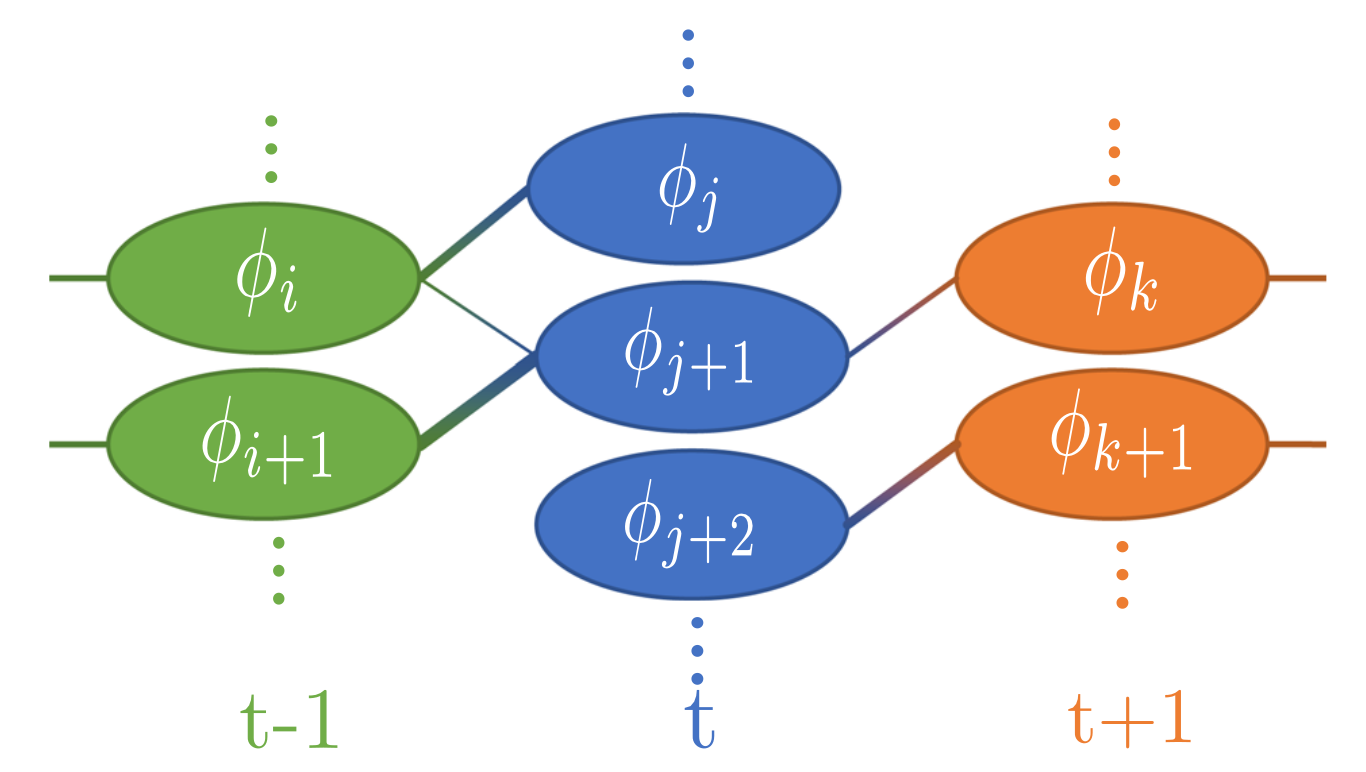
\includegraphics[width=0.8\textwidth]{ch2/similarity_graph.png}
    \caption{Ilustración conceptual del grafo de similitud que modela la dinámica de los tópicos en el tiempo. Un nodo corresponde a un tópico en una época específica; el ancho de los arcos es proporcional a la similitud entre los tópicos, arcos ausentes fueron eliminados por presentar una similitud menor a un umbral. Fuente:  Figura 3 de \citep{beykikhoshk2018discovering}}
    \label{img:graph}
\end{figure}

\subsection{Construcción automática del grafo de similitud}
\label{sec:automatic_construction}

Un aspecto relevante de esta metodología es definir el úmbral de corte, el cual no es fácilmente interpretable, además el úmbral depende de la médida de similitud escogida, dificultando así la comparación entre médidas de similitud. En \citep{beykikhoshk2018discovering} proponen una alternativa más interpretable para definir el úmbral, para esto estiman la función de densidad acumulada (cdf) del grafo inicial, donde todos los nodos de una época están conectados con todos los nodos de la época adyacente, al que llamaremos grafo \textit{fully connected}. \\

Sea $F_{p}$ la cdf sobre las similitudes del grafo inicial, luego sea $\zeta \in [0,1]$ el punto operante de la cdf, luego eliminamos el arco entre los tópicos $\phi_{t,i}$ y $\phi_{t+1,j}$ si $\rho(\phi_{t,i}, \phi_{t+1,j})\leq F_{p}^{-1}(\zeta)$, donde  $F_{p}^{-1}(\zeta)$ es el cuantil $\zeta$ de $F_{p}$. En \ref{img:cdf_sim} se tiene una ilustración para tres médidas de similitud, en esta se observa que la elección de un úmbral de corte arbitrario depende fuertemente de la médida de similitud escógida, por lo que la elección en base a la cdf puede ser más apropiada.

\begin{figure}
    \centering
    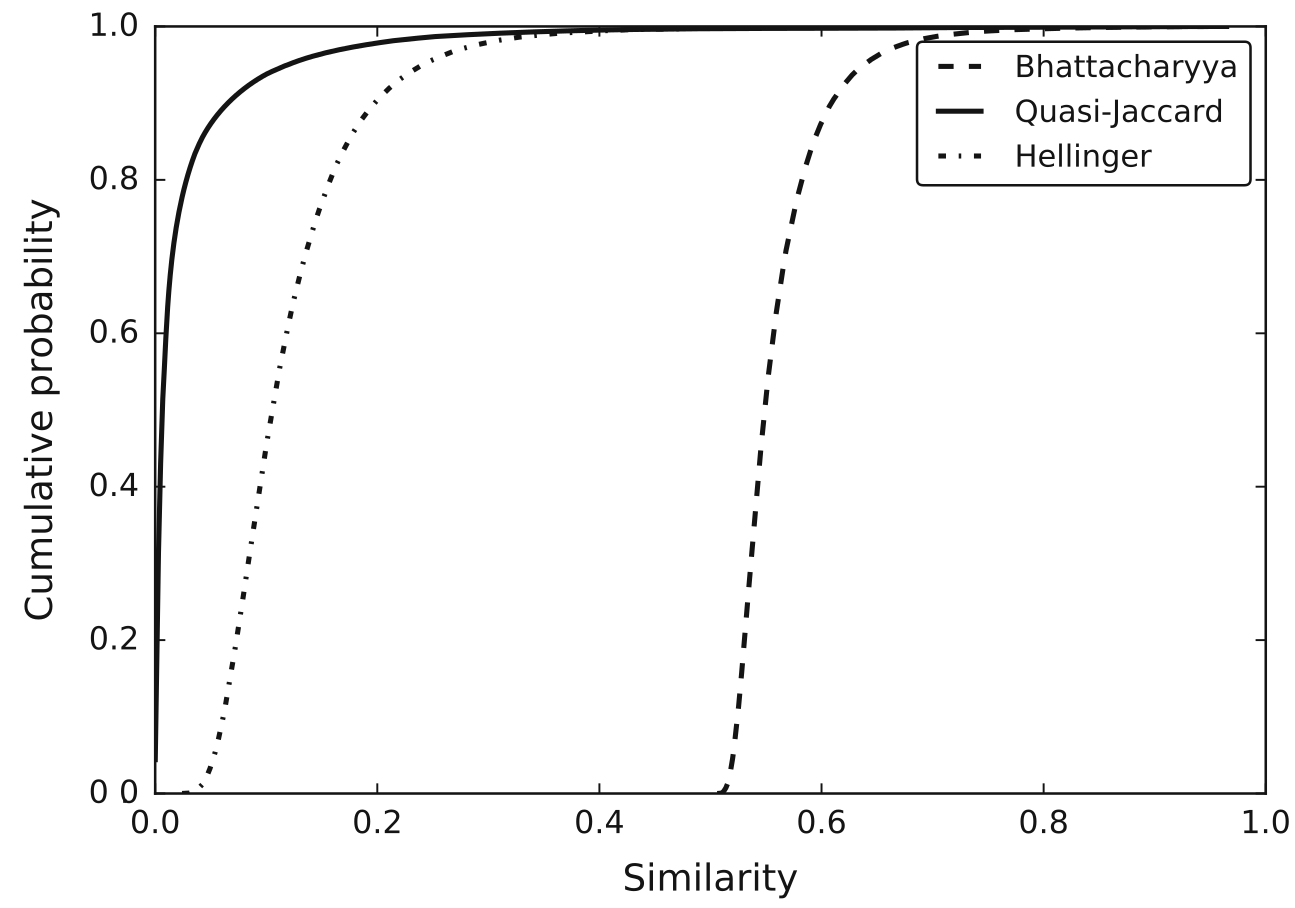
\includegraphics[width=0.8\textwidth]{ch2/cdf_sim.png}
    \caption{Estimación empírica de la función de densidad acumulada (cdf) de la similitud entre tópicos de épocas adyacentes en un grafo \textit{fully connected} para tres medidas de similitud. Fuente: Figura 4 \citep{beykikhoshk2018discovering}.}
    \label{img:cdf_sim}
\end{figure}


\chapter{Metodología}
\label{ch:methodology}
En este capítulo se describe la metodología propuesta para el descubrimiento de tópicos y su evolución en el tiempo. En la sección \ref{sec:processing} se describe la metodología de procesamiento usada para limpiar los datos, previa a la utilización del modelo de tópicos. En la sección \ref{sec:model_selected} se justifica la elección del modelo de tópicos, junto a la configuración de hiperparámetros usada y la herramienta a usar para facilitar su interpretación. Por último, en la sección \ref{sec:build_graph} se describe la metodología utilizada para modelar la evolución en el tiempo y la médida de similitud utilizada para comparar tópicos de épocas adyacentes.

\section{Procesamiento}
\label{sec:processing}

El proposito del procesamiento en \textit{text mining} es simplificar los datos lo más posible tal que se mantiene el \textit{core} de palabras del corpus. En el caso de modelamiento de tópicos, esta etapa puede reducir significativamente el vocabulario. Como consecuencia, esto puede traer una mejora en la significancia estadística de los modelos, puesto que se puede obtener un mejor balance entre cantidad de parámetros y observaciones. Adicionalmente, puede facilitar la interpretación de los tópicos, removiendo palabras que aportan poca información.\\

En este experimento se aplicaron cinco etapas:
\begin{enumerate}
\item \textbf{Tokenización}: La tokenización es una operación sobre una cadena de caracteres (\textit{string}) que consiste en dividir el \textit{string} (ej: por el caracter espacio) en un conjunto de términos, obteniéndose así una lista elementos llamados \textit{tokens}, que en términos simples pueden considerarse como una palabra.
\item \textbf{Procesamiento de caracteres}: En esta etapa se suelen aplicar algunas operaciones básicas de procesamiento. En este proceso se llevan los tokens a unicode y minúsculas. Luego, se eliminan patrones de caracteres que difícilmente pueden tener algún significado, como correos electrónicos, símbolos de puntuación, tokens con números y letras o solo números. 
\item \textbf{Eliminación de stopwords}: Las \textit{stopwords} \citep{wilbur1992automatic} son palabras que aportan poca información (ej: artículos, preposiciones y conectores), usualmente tienen un alta frecuencia dentro del corpus. Para esto se utiliza una lista de palabras de \textit{stopwords} disponible en el paquete NLTK de Python de 313 palabras \citep{bird2009natural}. Además, esta lista se alimenta con 951 \textit{stopwords} contextuales, palabras específicas del corpus que aportan poca información, en el caso del robo de vehículos palabras relacionas a \quotes{robo} o \quotes{vehículo} no aportan ninguna información, puesto a que todos los relatos hablan del robo de un vehículo. 
\item \textbf{Filtro por vocabulario}: Con el proposito de mantener las palabras que son \quotes{humanamente legibles} se utiliza un vocabulario. Para esto se utilizó el vocabulario del corpus SUC descrito en la sección anterior, de esta menera toda palabra tiene su \textit{word embedding}. 
\item \textbf{Filtro por frecuencia}: En este nivel se eliminan los \textit{tokens} con baja frecuencia. Esta etapa viene motivada del hecho de que un modelo difícilmente aprenderá algún patrón de un evento que tiene muy pocas realizaciones, menos si tiene una realización única. Esta etapa se aplica a nivel epoca, eliminando aquellos tokens que aparecen en menos del 0.1\% de los documentos de su respectiva época.
\item \textbf{Eliminación de documentos}: En el último nivel se eliminan aquellos documentos que presentan pocos tokens, eliminando documentos que presentan menos de 5 tokens. Esto tiene por objetivo obtener estimaciones más confiables y reducir la posibilidad de sacar conclusiones prematuras debido a las pocas observaciones con las que cuenta un documento. 
\end{enumerate}

\section{Modelos de tópicos}
\label{sec:model_selected}

Se escoge HDP como modelo de tópicos base de la metodología. Si bien, HDP es un modelo similar en estructura a LDA, cuenta con la ventaja de que el número de tópicos no está acotado y es inferido a partir de los datos, en cambio LDA requiere de escoger el número de tópicos $K$ por adelantado. \\

En un enfoque tradicional, se requiere de entrenar múltiples veces LDA para diferentes valores de $K$ y se escoge la configuración con mejor desempeño en un conjunto de validación, por lo que LDA termina siendo computacionalmente más costoso que HDP, además este enfoque se vuelve impracticable cuando el conjunto de datos es lo suficientemente grande. \\

En el aspecto cualitativo ambos modelos entregan tópicos igual de consistentes. En cuanto a métricas de desempeño como $\textit{perplexity}$ HDP suele tener mejor desempeño \citep{teh2005sharing}.\\

Para el descubrimiento de tópicos se utilizó la implementación disponible en C++ \citep{HDP} de HDP para modelamiento de tópicos. Esta implementación está basada en el algoritmo de Gibbs Sampling propuesto en \citep{teh2005sharing}.

\subsection{Configuración de hiperparámetros}
\label{sec:hdp_hiperparameters}

HDP tiene tres hiperparámertos, el parámetro de concentración a nivel corpus $\gamma$, el parámetro de concentración a nivel documento $\alpha_{0}$ y $\eta$ el parámetro de la medida base Dirichlet.\\

En modelamiento de tópicos se prefiere usar $\eta\in (0,1)$, esto generará distribuciones \textit{sparse} sobre el vocabulario. Así, se suelen tener tópicos más distinguibles, donde el \textit{core} de palabras del tópico concentra la masa de la distribución. Además, como la semántica del tópico está compactada en pocas palabras se facilita la interpretación. En este caso se utilizó un punto intermedio, fijando $\eta=0.5$.\\ 

\begin{figure}
    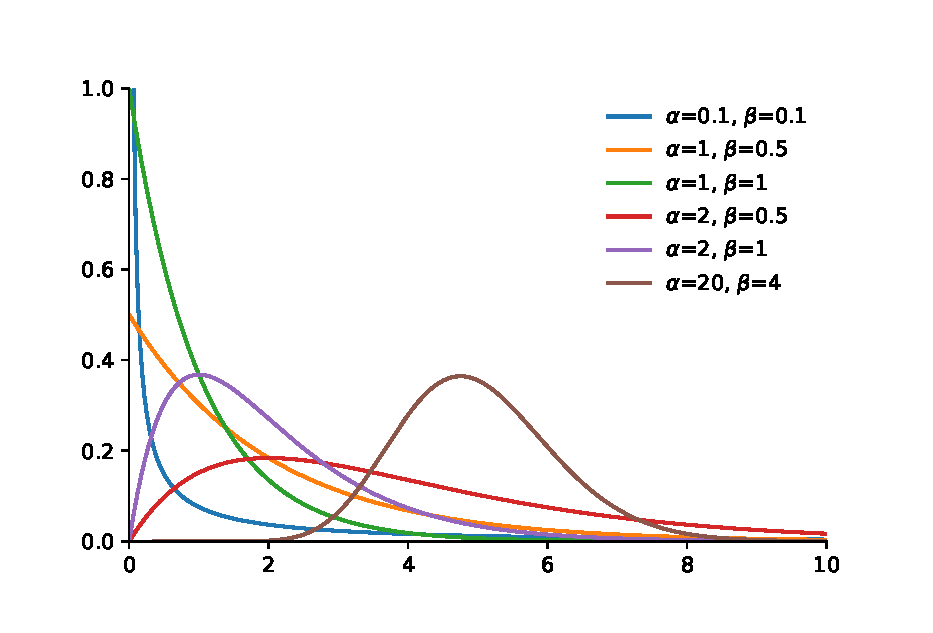
\includegraphics[width=0.8\textwidth]{ch3/gamma.eps}
    \caption{Función de densidad de probabilidad (pdf) de una distribución Gamma para diferentes parámetros de forma $\alpha$ y tasa $\beta$.}
    \label{img:gamma}
\end{figure}

En \citep{teh2005sharing} los parámetros de concentración se integran afuera usando un prior \textit{vague gamma} \citep{escobar1995bayesian}. Un prior \textit{vague gamma} es una distribución Gamma con una gran parte de la masa en torno a cero y una cola pesada (ver Figura \ref{img:gamma} para una ilustración de la pdf para diferentes parámetros). Por consecuencia, el prior tendrá un menor efecto de regularización y a medida que más datos se obtienen la posterior conincidirá con las observaciones empíricas. En este caso se utilizó un prior $\Gamma(\alpha=1, \beta=1)$.

\subsection{Interpretación de tópicos}

Los modelos de tópicos probabilísticos se caracterizan por tener un alto poder interpretativo, esto se debe a que la distribución de probabilidad de cada tópico sobre el vocabulario nos da una idea del tema al que pertenece, por otro lado, la mezcla de tópicos de cada documento nos muestra que tan importante es cada tópico en la generación de estos, como también dentro del corpus. \\

En este sentido, las visualizaciones nos pueden ayudar a interpretar mejor los resultados de los modelos de tópicos. Para la interpretación de los tópicos la metodología propuesta se basa en la herramienta de visualización desarrollada en  \citep{sievert2014ldavis}, la cual responde las siguientes preguntas, ¿Cuál es el significado de cada tópico?¿Cuán predominante es cada tópico?¿Cómo se relacionan los tópicos entre sí?\\

Para responder la pregunta 1 se incorpora un gráfico de barras que muestra las palabras más relevantes del tópico seleccionado dado un parámetro $\lambda \in [0,1]$. A través de una visualización espacial responde la pregunta 2 y 3. La visualización espacial consiste en aplicar técnicas de reducción de dimensionalidad como TSNE \citep{maaten2008visualizing} o PCA \citep{wold1987principal} (en este caso se utilizó TSNE) a la matriz de distancia entre tópicos, usando Jensen-Shannon divergence \citep{endres2003new} como médida de distancia. Una vez cada tópico es mapeado a un punto en un espacio de dos dimensiones se dibuja un círculo con centro en este punto y con radio proporcional a la cantidad de tokens generados por el tópico.\\
% se podría meter mano para reemplazar por WMD, en ese caso mover a una sección posterior

Para interpretar un tópico, lo usual es examinar una lista ordenada de las palabras más probables del tópico, usando ya sea desde cinco a treinta términos. Un problema frecuente que se presenta en este caso es que los términos que son comunes al corpus frecuentemente aparecen en el top de las palabras más probables de un tópico, haciendo difícil discernir el significado de estos. Para esto en \citep{sievert2014ldavis} se define una métrica denominada \textit{relevance}, la cual define la relevancia de una palabra no solo por su probabilidad dentro del tópico sino también por su exclusivad dentro del corpus. La \textit{relevance} de una palabra $w$ en el tópico $k$ dado $\lambda$ está dada a través de la siguiente expresión:

\begin{align}
    r(w,k|\lambda) = \lambda log (\phi_{kw})+ (1-\lambda)\lambda log\bigg(\frac{\phi_{kw}}{p_{w}}\bigg)
\end{align}

, donde $\lambda$ determina el peso que se le da a la probabilidad de la palabra $w$ dentro del tópico $k$ ($\phi_{kw}$) relativo a su \textit{lift}, el cual se define por el ratio entre la probabilidad de la palabra dentro del tópico y su probabilidad marginal a lo largo del corpus ($p_w$). Fijando $\lambda=1$ se obtiene el ranking de términos decrecientes en orden de su probabilidad dentro del tópico, y fijando $\lambda=0$ el ranking se basa solo en el \textit{lift}.

\section{Construcción del grafo temporal}
\label{sec:build_graph}

Nuestro objetivo no es solo descubrir tópicos sino también modelar sus interacciones en el tiempo, como nacimiento, muerte, evolución, divisón y fusión.
Así, la metodología propuesta se basa en la metodología descrita en la sección \ref{sec:similarity_graph} propuesta en \citep{beykikhoshk2018discovering}, debido que esta captura los dinamismos mencionados.\\

En general las medidas de similitud o distancia comparan vectores con el mismo dominio y dimensión, esto significa que los tópicos de épocas adyacentes deben compartir el mismo vocabulario. Matemáticamente, sea $\phi_{t, i}$ un tópico de la época $t$ y $V_{t}$ su vocabulario, sea  $\phi_{t+1, j}$ un tópico de la época $t+1$ y $V_{t+1}$ su vocabulario. Con una alta probabilidad existan palabras en $V_{t}$ que no están en $V_{t+1}$ y viceversa. Para poder comparar tópicos en épocas adyacentes se debe construir un vocabulario global $V_{t+1}^{'}=V_{t}\cup V_{t+1}$, luego aplicar $padding$ a los vectores $\phi_{t, i}$ y $\phi_{t+1, j}$, es decir, rellenar con ceros las posiciones que no están en el vocabulario de su dominio.\\

Una gran desventaja del enfoque anterior es que no captura similitud entre palabras, puesto que cada palabra ocupa una posición dentro del vector y no hay forma de comparar palabras que no son comúnes en ambas épocas. El peor caso sería considerar los vocabularios $V_{t}$ y $V_{t+1}$, con $V_{t}\cap V_{t+1} =  \emptyset$, a pesar de que cada palabra en $V_{t}$ tiene un sinónimo en $V_{t+1}$ la similitud entre tópicos entre las épocas $t$ y $t+1$ sería cero.\\

\subsection{Word Mover's Distance}

Para lidiar con el problema anterior, se propone utilizar una medida de distancia conocida como Word Mover's Distance (WMD) \citep{kusner2015word}, medida utilizada para comparar dos documento bajo una representación \textit{bag of words} a través de sus \textit{word embeddings} \citep{mikolov2013distributed}.\\

WMD calcula el costo mínimo de transformar un documento en otro, en esto caso particular sería el costo mínimo de llevar un tópico a otro. Para esto se resuelve el problema de transporte, donde los flujos son los pesos $\phi_{t,i}$ y $\phi_{t+1,j}$ y la matriz de costos es una matriz de distancia euclidiana entre los \textit{word embedding} de todas las palabras deS $V_{t}$ con $V_{t+1}$. En la Figura \ref{img:wmd_obama} se ilustra el espacio en el que viven las palabras de dos documentos.

\begin{figure}
    \centering
    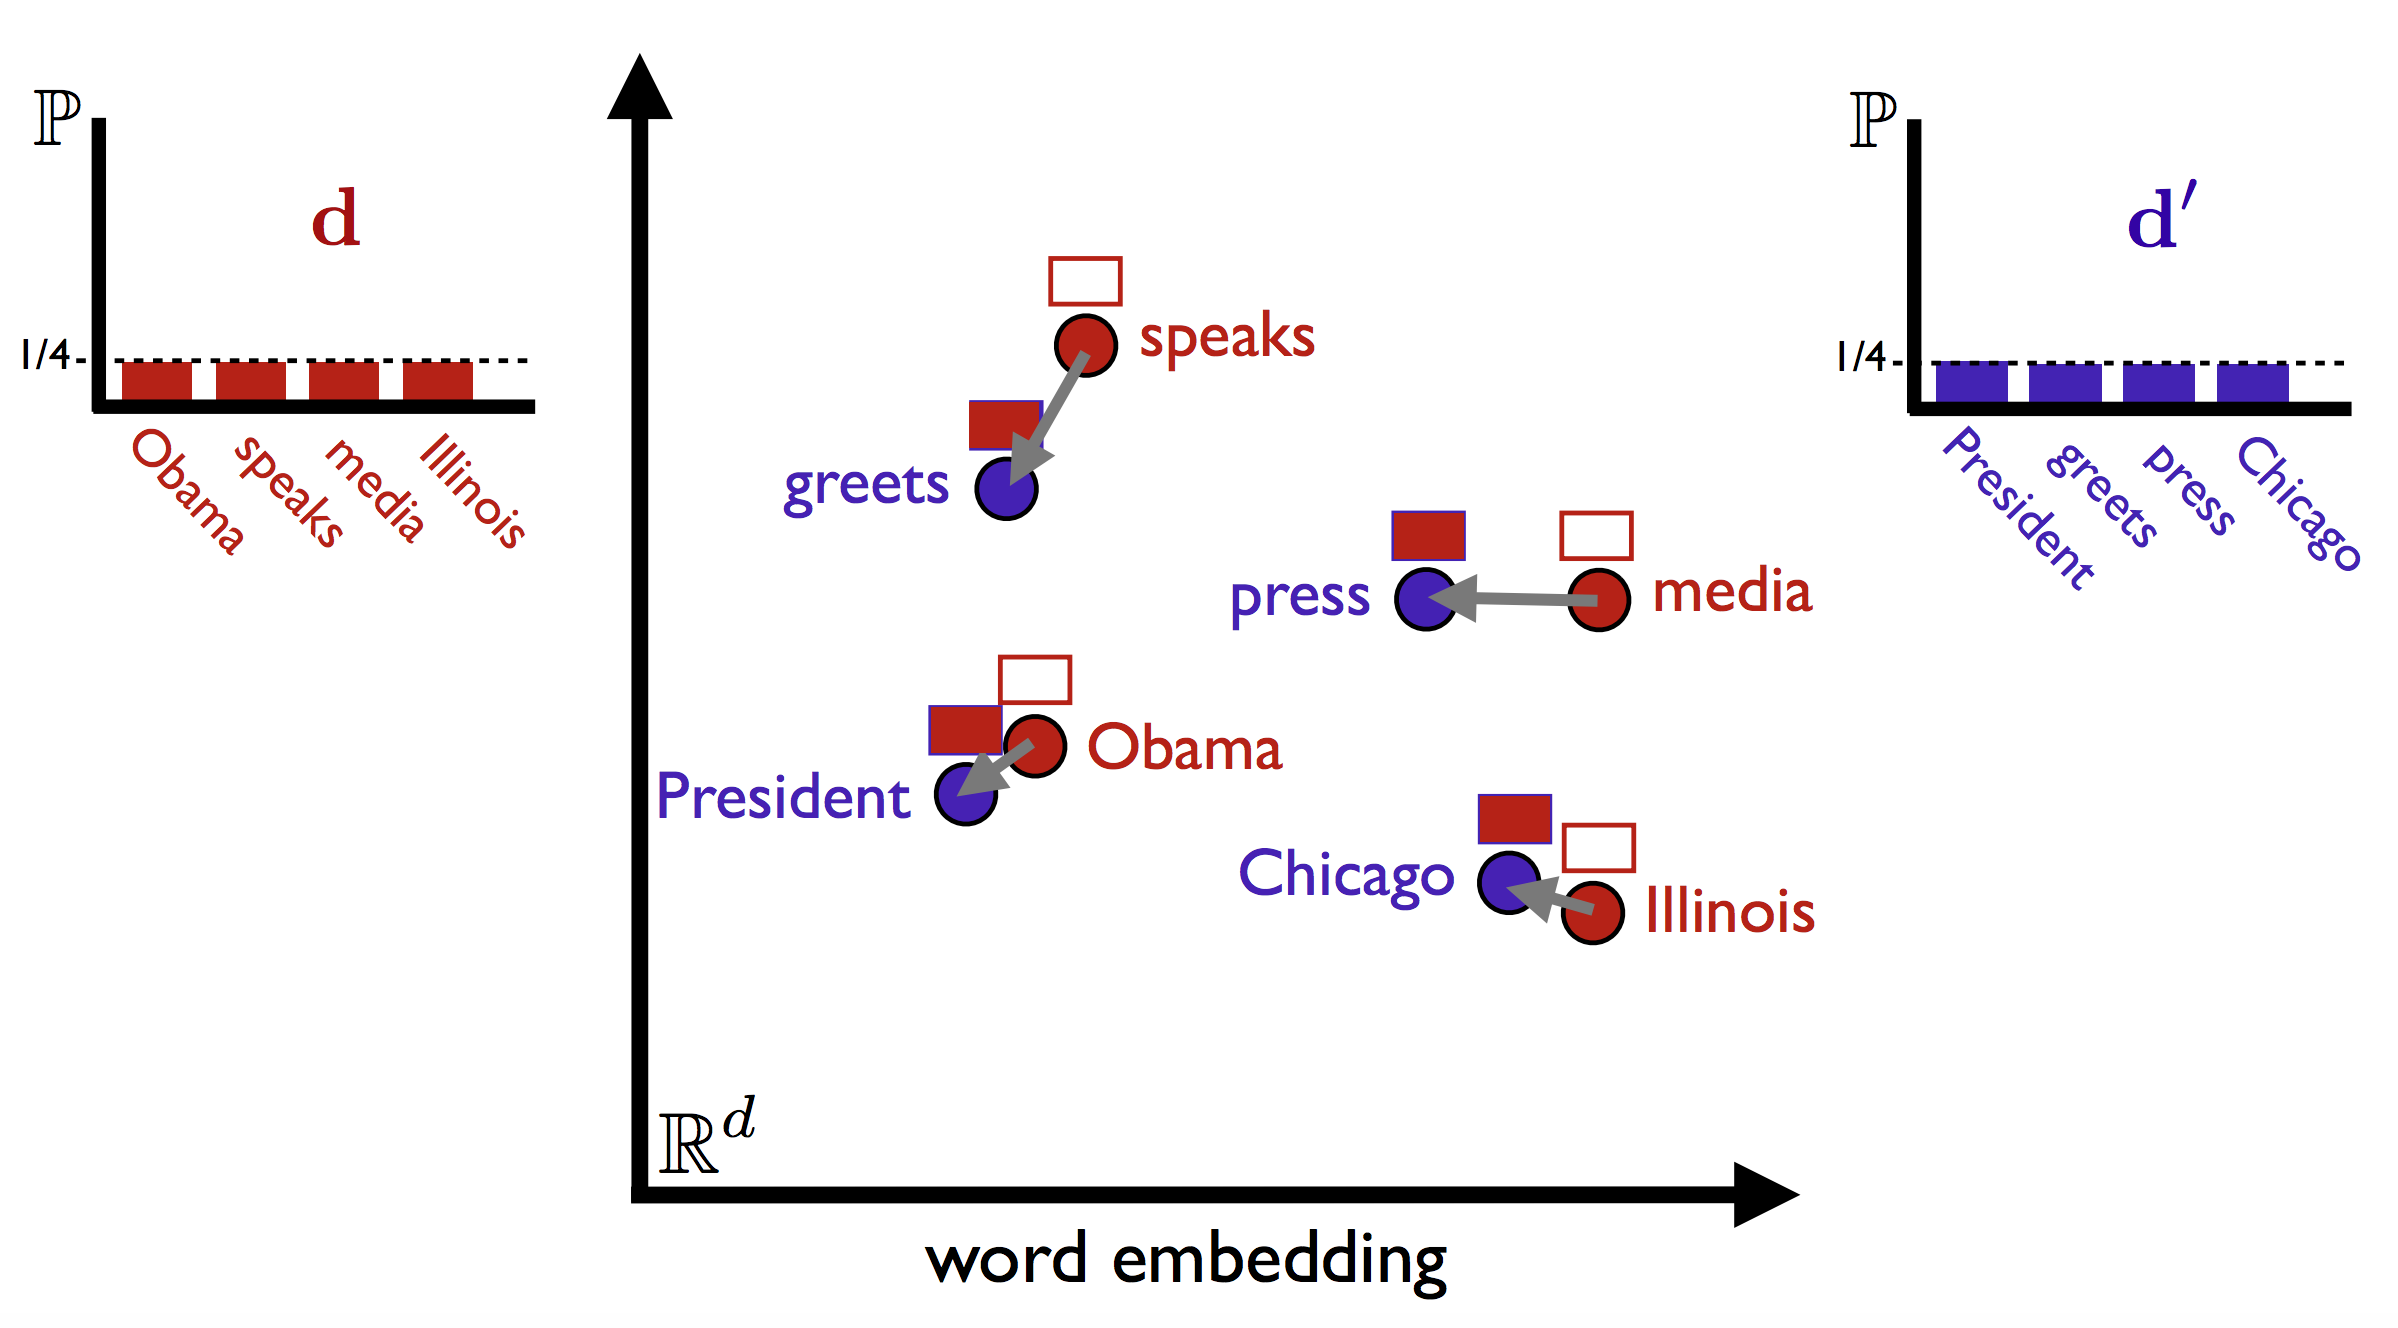
\includegraphics[width=1\textwidth]{ch3/wmd-obama.png}
    \caption{Espacio vectorial de los \textit{word embeddings} de las palabras de dos documentos con un vocabulario de tamaño 4. Fuente: Figura de \citep{WMDPy}.}
    \label{img:wmd_obama}
\end{figure}

Sea  $V_{i}$ y $V_{j}$ los vocabularios del tópico $i$ y $j$ respectivamente, luego su WMD viene dado por $WMD(\phi_{i}, \phi_{j})$:

\begin{align}
\underset{x}{\text{min}}&\sum_{u \in V_{i}}\sum_{v \in V_{j}} c_{u,v}x_{u,v} \\ 
\textrm{s.t.} &\sum_{v \in V_{j}}x_{u,v}= \phi_{i,u}, \; u \in V_{i}\\ 
& \sum_{u \in V_{i}}x_{u,v}= \phi_{j,v}, \; v\in V_{j}\\
& x_{u,v} \geq 0,\; u \in V_{i} \;, v \in V_{j}\\ \nonumber
\end{align}

Donde $x_{u,v}$ es el flujo que va de la palabra $u$ del tópico $i$ a la palabra $v$ del tópico $j$, $\phi_{i,u}$ es la probabilidad de la palabra $u$ en el tópico $i$, $c_{u,v}$ es el costo de mover una unidad de flujo por el arco $(u,v)$, el costo entre palabras se mide como la distancia euclidiana entre los \textit{word embedding} de dichas palabras.\\

La primera restricción indica que el flujo que se mueve de una palabra $u$ del tópico $i$ a todas las palabras del tópico $j$ debe sumar su peso ($\phi_{i,u}$), la segunda restricción significa que el flujo que se mueve de una palabra $v$ del tópico $j$ a todas las palabras del tópico $i$ debe sumar su peso ($\phi_{j,v}$). Lo anterior implica que esta medida de distancia es simétrica, es decir, $WMD(\phi_{i}, \phi_{j}) = WMD(\phi_{j}, \phi_{i})$.\\

WMD se puede fácilmente transformar en una médida de similitud, $\rho(\phi_{i}, \phi_{j}) = \frac{1}{1+WMD(\phi_{i}, \phi_{j})}$, notar que si la WMD es 0 la similitud es 1 y si es $\infty$ la similitud es 0. \\

\subsection{WMD complejidad}

WMD es una medida de distancia intensiva en recursos computacionales. Para entender mejor esto utilizaremos la representación poliedral del problema, sea $N$ el tamaño del vocabulario entre dos épocas adyacentes, luego la región factible del problema anterior se puede representar como $\{x| Ax=b, x\geq 0\}$ sobre un grafo bipartito, con $A\in \mathbb{R}^{2N\times N^{2}}$ la matriz de incidencia, $b\in \mathbb{R}^{2N}$ la capacidad de los nodos y $x\in \mathbb{R}^{N}$ el flujo a enviar por cada uno de los arcos. Para resolver este problema se utilizó \citep{PyEMD}, la cual está basada en el algoritmo \citep{pele2009fast}, cuya complejidad del mejor tiempo promedio escala $\mathcal{O}(N^{2}log N)$.\\

Los tópicos siguen una distribución con forma de ley de potencia sobre el vocabulario, donde una pequeña fracción de las palabras concentran la mayor parte de la masa de la distribución. Además, en la práctica la interpretación de los tópicos se basa en los top $N$ palabras más probables con $N \in [5, 30]$, entonces, podemos aprovechar esta estructura para efectos de computar la WMD de un forma más eficiente, por ejemplo, utilizando solo las palabras que capturan un X\% de la distribución acumulada del tópico. De hecho si se reduce el vocabulario a un décimo esto traera en el peor caso promedio un \textit{speed up} de 200.\\

\subsection{Word Embeddings}

Computar WMD requiere contar con \textit{word embeddings}. Para estó se utilizó una de las más grandes colecciones de \textit{word embeddings} en español \citep{fastextSUC}, que cuenta con 1.313.423 \textit{embeddings}, colección obtenida utilizando el algoritmo FasText \citep{bojanowski2017enriching} sobre el corpus Spanish Unannotated Corpora (SUC) \citep{josecanneteSUC}, uno de los más grandes corpus de texto en español. FasText en comparación a otros enfoques para extraer \textit{embeddings} representa los \textit{tokens} a través de n-gramas de caracteres, de esta manera se pueden obtener \textit{embeddings} de \textit{tokens} no vistos durante el entrenamiento a partir de los \textit{embeddings} de los caracteres que lo componen.

\subsection{Métricas}

En la metodología propuesta podemos considerar dos fuentes de evaluación de desempeño, el descubrimiento de tópicos y cómo se relacionan. En ambos casos no se cuenta con el \textit{ground truth} para medir correctamente el desempeño. Si conocieramos el \textit{ground truth}, podríamos utilizar \textit{purity} \citep{manning2008introduction} para comparar la asignación de los documentos en torno a los tópicos con la etiqueta. En el caso del grafo temporal, si conocieramos las conexiones presentes y ausentes podríamos utilizar métricas de clasificación.\\

En \citep{blei2003latent,griffiths2004finding,cao2009density,arun2010finding,deveaud2014accurate,zhang2017lda} se describen algunas métricas que no requieren de una etiqueta, que pueden ser útil para realizar selección de modelo de tópico. Cabe destacar que estas métricas carecen de significado y sirven para comparar si un modelo de tópicos es superior a otro.\\

El trabajo propuesto no tiene por objetivo calibrar los hiperparámetros del HDP y se utilizó la configuración especificada en la sección \ref{sec:hdp_hiperparameters}. Por el contrario, se enfoca en medir el desempeño de las interacciones entre los tópicos descubiertos, asumiendo que los tópicos descubiertos están correctos. El desempeño es medido mediante métricas de clasificación sobre un grafo etiquetado. Esto es posible  debido a que el fenómeno de robo de vehículos no presenta muchos tópicos a diferencia de los tópicos latentes que podríamos encontrar en Wikipedia.\\

La métrica escogida en este caso es el \textit{macro average recall} \citep{forman2003extensive}, esta corresponde al promedio simple entre la tasa de aciertos de la clase presencia y ausencia de conexión. En general, debería haber más ausencia que presencia de conexión, así bajo esta métrica la clase presencia de conexión no será menospreciada, ya que el macro recall considera que el tasa de acertividad de ambas clases son igual de importantes.\\

Adicionalmente, al contar con un grafo etiquetado podemos observar el efecto de los hiperparámetros $\zeta$ y $q$ en la métrica de desempeño escogida. El hiperparámetro $\zeta\in[0,1]$ define el úmbral de corte, representa el punto operante de la cdf del grafo \textit{fully connected}, permite definir el cuantil que se usará como úmbral para eliminar arcos con similitud menor a este. El parámetro $q \in [0,1]$ define el soporte de los tópicos, utilizando aquellas palabras más probables que explican 100q\% de la distribución acumulada del tópico. 

\section{Resumen metodología}

En la Figura \ref{img:scheme} se presenta un esquema que resume de la metodología propuesta para el descubrimiento y seguimiento de tópicos en el tiempo. El primer proceso de la metodología corresponde al procesamiento, el cual toma el corpus original y lo divide en épocas, luego a nivel época se aplican cinco niveles de procesamiento de forma secuencial: tokenización, procesamiento de caracteres, eliminación de \textit{stopwords}, filtro por vocabulario y filtro por frecuencia. Como producto del proceso anterior se obtiene un corpus listo para la aplicación de algún modelo de tópicos, en este caso corresponde al modelo HDP, el cual se aplica de forma independiente sobre cada una de las épocas. Por último, una vez descubiertos los tópicos se procede a construir el grafo temporal, para esto es necesario computar la WMD entre los tópicos de épocas adyacentes, luego se podan los arcos cuya similitud es menor al cuantil $\zeta$ de la distribución acumulada del grafo \textit{fully connected}.

\def\db[#1,#2,#3,#4,#5]#6{%
  \node[draw, cylinder, alias=cyl, shape border rotate=90, aspect=#3, %
  minimum height=#1, minimum width=#2, outer sep=-0.5, color=black] (#4) at #5 {};%
  \node at #5 {#6};%
}
\def\boxtext[#1,#2,#3,#4,#5]#6{
        \node[draw=black, rounded corners, minimum height=#1,minimum width=#2, text width=6em] (#4) at #5 {}; 
        \node[anchor=#3,inner sep=4pt,] at (#4.#3)  {#6};
}
\def\isaedge[#1,#2,#3,#4];{ 
  \draw[-triangle 60,color=black!20!black,#4,fill=white] (#1) -- #3
  (#2);  
}

\begin{figure}
\begin{tikzpicture}
\db[45,40,1.6,db1,(0,2.2)] {
    \scriptsize\begin{tabular}{l}
        Corpus\\
        Original
    \end{tabular}
};
\boxtext[220,120,north,p,(3.5,2.2)] {\textbf{Procesamiento}};
\isaedge[db1,p,,];
\boxtext[180,100,south,p0,(3.5,2)] {$1:T$};
\boxtext[15,20,north,p1,(3.5,4.6)] {\footnotesize Tokenización};
\boxtext[15,20,north,p2,(3.5,3.4)]{\footnotesize Caracteres};
\boxtext[15,20,north,p3,(3.5,2.2)]{\footnotesize Stopwords};
\boxtext[15,20,north,p4,(3.5,1.0)]{\footnotesize Vocabulario};
\boxtext[15,20,north,p5,(3.5,-0.2)]{\footnotesize Frecuencia};
\isaedge[p1,p2,,];
\isaedge[p2,p3,,];
\isaedge[p3,p4,,];
\isaedge[p4,p5,,];
\db[45,40,1.6,db2,(7,2.2)] {
    \scriptsize\begin{tabular}{l}
        Corpus\\
        Procesado
    \end{tabular}
};
\isaedge[p,db2,,];
\boxtext[50,50,north,hdp,(9.7,2.2)] { 
    \begin{tabular}{l}
        \textbf{Tópicos}\\
        HDP $1:T$
    \end{tabular}
};
\isaedge[db2,hdp,,];
\boxtext[80,100,north,g,(13.5,2.2)] {\textbf{Grafo Temporal}};
\isaedge[hdp,g,,];
\boxtext[15,40,north,g1,(13.5,2.6)]{\footnotesize WMD};
\boxtext[15,40,north,g2,(13.5,1.4)]{\footnotesize Prunning};
\isaedge[g1,g2,,];
\end{tikzpicture}
\caption{Esquema de la metodología de descubrimiento y evolución de tópicos.}
\label{img:scheme}
\end{figure}

\chapter{Caso de estudio}
\label{ch:case_study}
En este capítulo se analizan los resultados de la metodología propuesta al fenómeno de robo de vehículos. En la sección \ref{sec:data} se describe la fuente de información utilizada. En la sección \ref{sec:data_processing} los resultados del procesamiento de los datos. Por último, en la sección \ref{sec:quantative}-\ref{sec:qualitative} se realiza un análisis cuantitativo y cualitativo de los resultados.

\section{Datos}
\label{sec:data}

Para este experimento se cuenta con relatos de víctimas del robo de vehículos provistos por la Asociación de Aseguradores de Chile (AACH). Esta base de datos consta con 49,015 relatos entre los años 2011-2016, veasé la Figura \ref{img:robberies_aach} para el detalle por año.

\begin{figure}
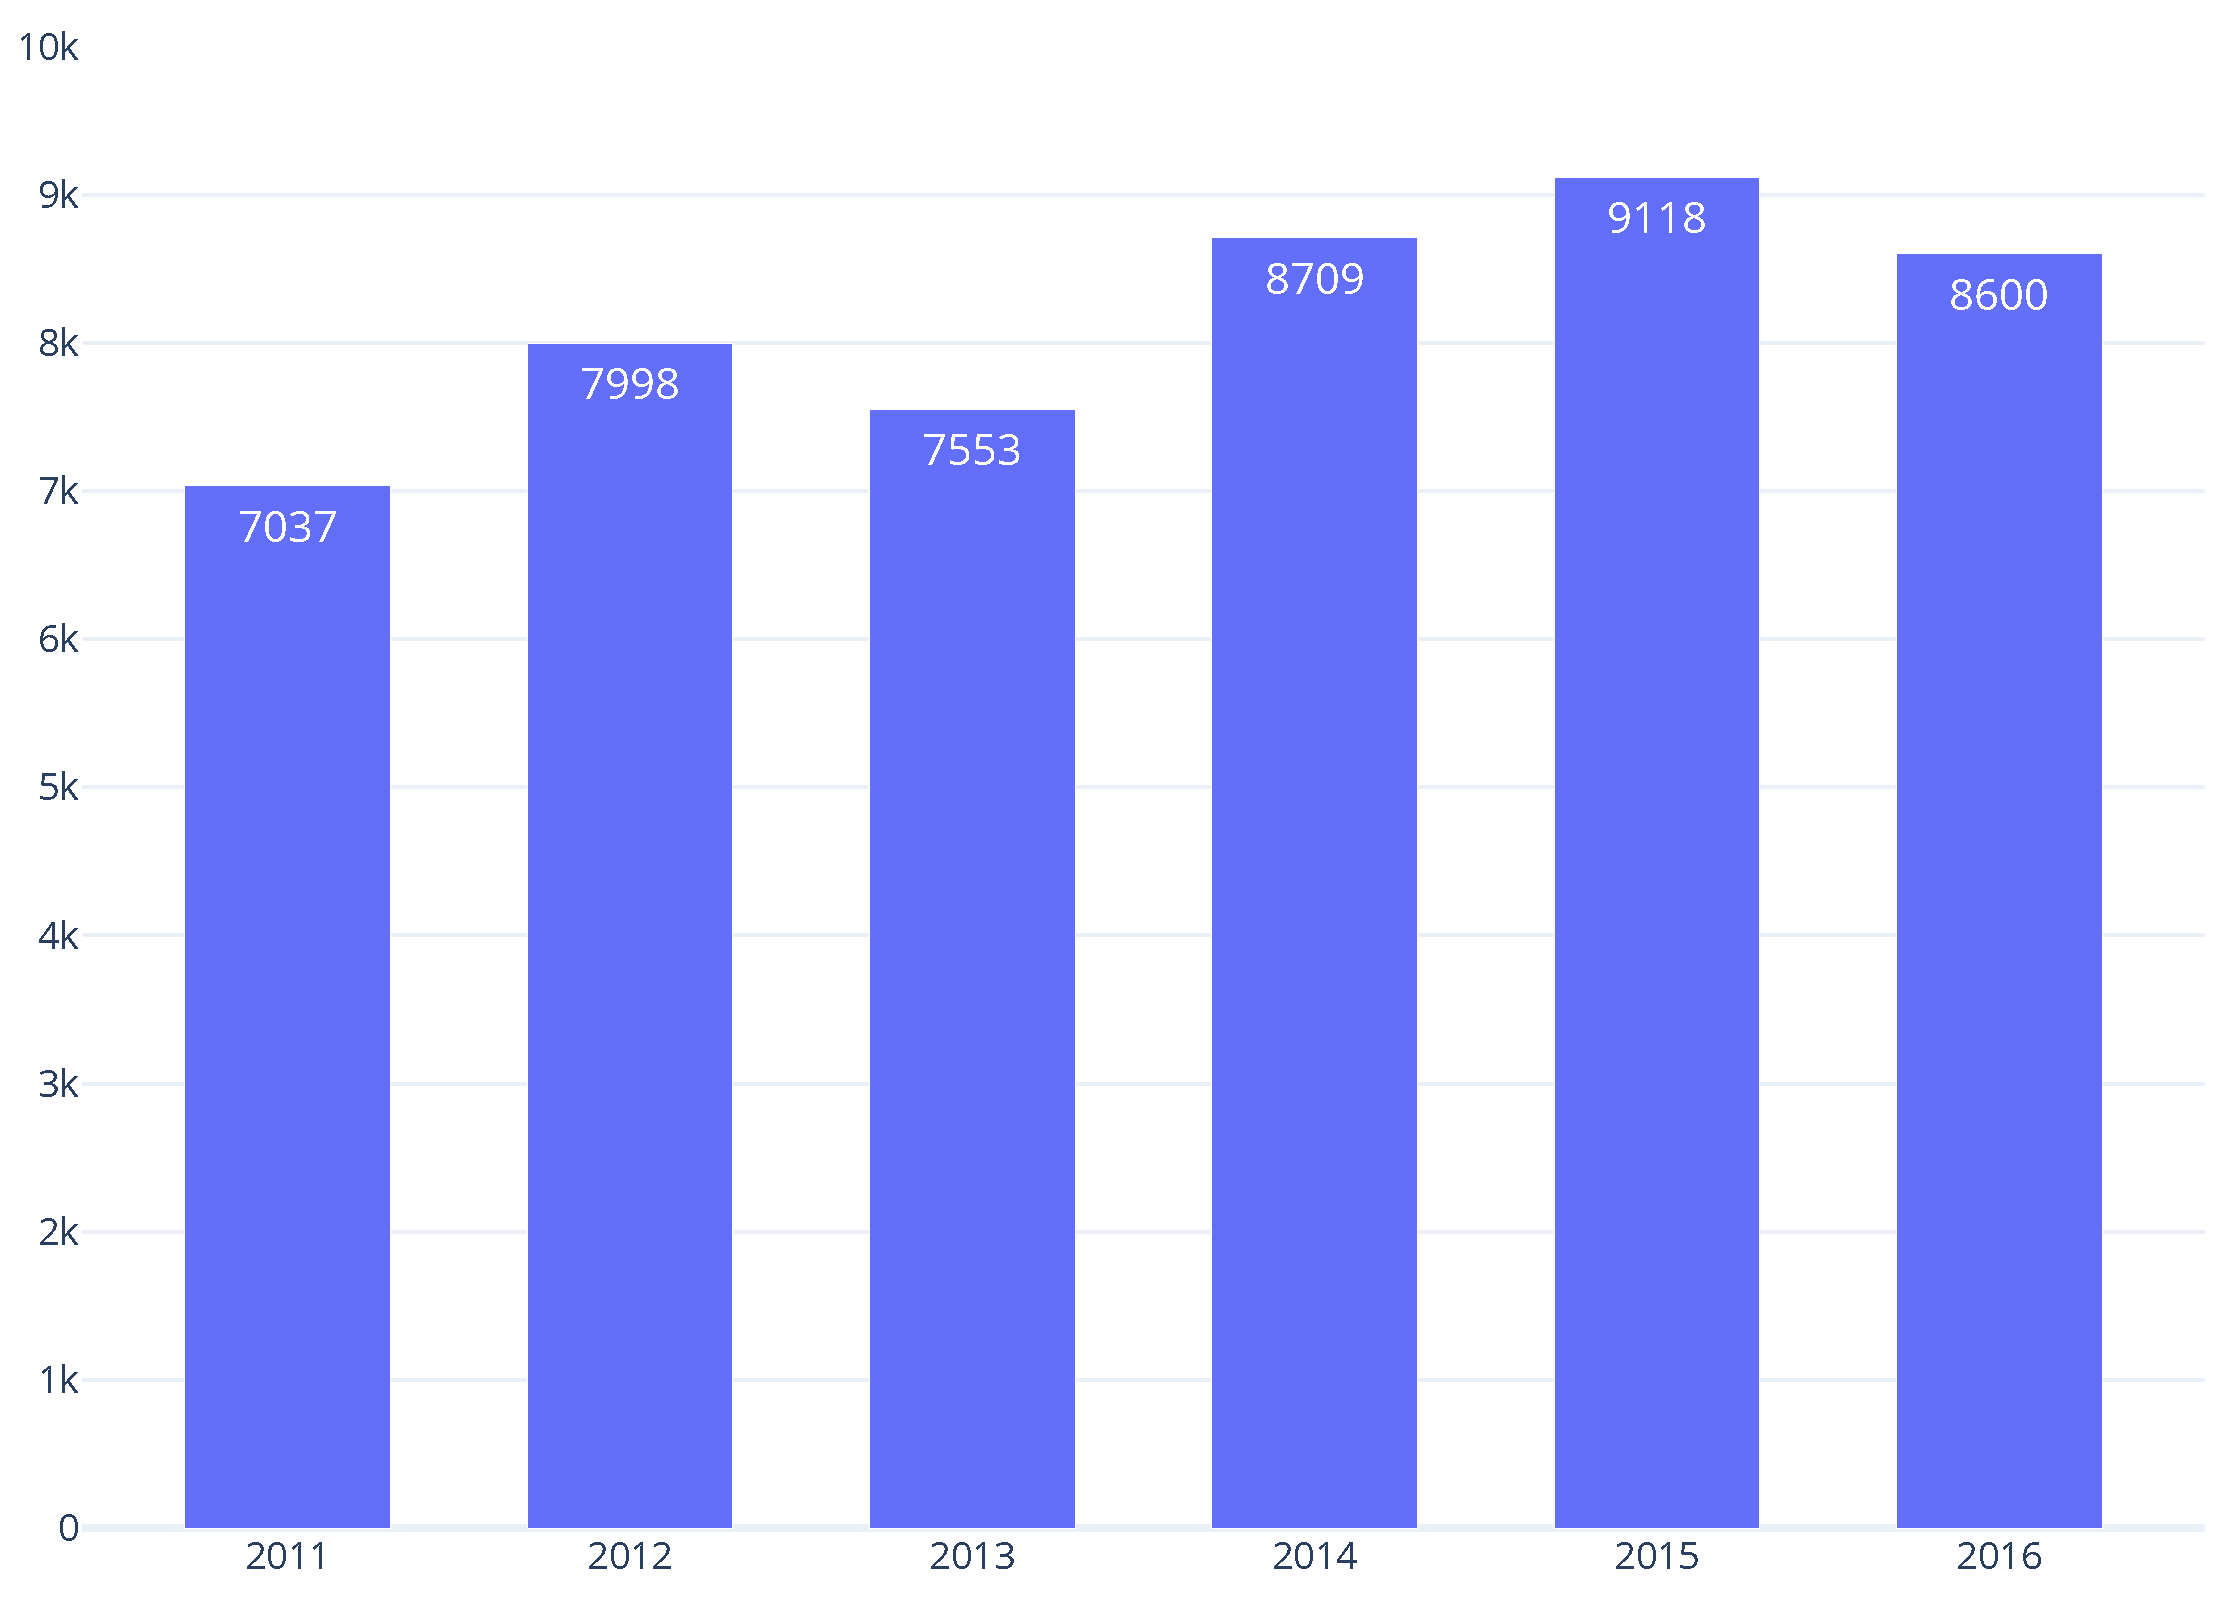
\includegraphics[width=0.8\textwidth]{ch4/robberies_aach.eps}
\caption{Cantidad de robos registrados por año en base de datos AACH.}
\label{img:robberies_aach}
\end{figure}

En la Figura \ref{img:documents} se muestra algunos ejemplos de la base de datos de la AACH, de aquí se observa que los relatos carecen de estandarización y presentan múltiples errores ortográficos. En consecuencia, la etapa de procesamiento toma suma relevancia, ya que aplicar un modelo de tópicos a un corpus sin ningún tipo de procesamiento puede llevar a resultados no deseados. En la sección \ref{sec:data_processing} se detallan los resultados obtenidos sobre el corpus tras aplicar los niveles de procesamiento mencionados en la sección \ref{sec:processing}.

\def\grayboxtext[#1,#2]#3{
        \node[fill=gray!80, text width=36em, draw=black!80, rounded corners, align=justify, below=#1] (#2) {#3}; 
}
\begin{figure}
\begin{tikzpicture}
    \grayboxtext[,t1]{\small ESTABA ESTACIONADO EL LA CALLE ROTEMBURGO ENTRE NORUGA Y SEÑORA DEL ROSAIO  Y AL MOMENTO DE IR A BUSCAR EL AUTO SE DA CUENTA QUE EL VH NO SE ENCUETRA AL PARECER LO ROBARON. NO POSEEE LOS DOCUMENTOS DEL VH vh aparece pero con mulples daños e evaluar queda en manos del liquidador.};
    \grayboxtext[0.2cm of t1,t2]{\small ME ENCONTRABA CARGANDO COMBUSTIBLE EN LA SHELL DE CARRASCAL CON WALKER MARTÍNEZ Y REPENTINAMENTE FUI ASALTADA EN FORMA VIOLENTA LLEVASE MI VEH (TENGO GRABACIÓN ). DAÑOS: ROBO DE MI VEH . LEIVA SE DERIVA A DON MARIO MEDINA .3 UF.DED/XX@XX.CL};
    \grayboxtext[0.2cm of t2,t3]{\small TEXT : DEJO MI VEHICULO ESTACIONADO EN DICHO LUGAR AL VOLVER ME PERCATO QUE EL VEHICULO HABIA SIDO ROBADO  EL MISMO DIA DEL ROBO A LAS 20:00 SOY CONTACTADO POR CARABINEROS DE LA COMUNA DE EL BOSQUE LOS CUALES ME INFORMAN QUE HABIAN RECUPERADO MI VEHICULO EL CUAL PRESENTABA LOS SIGUIENTES DAÑOS : VIDRIO TRASERO DERECHO QUEBRADA  CHAPA DE CONTACTO FORZADA  PARACHOQUE DELANTERO DERECHO RAYADO  ALARMADESCONECTADA  OTROS DAÑOS EN EL SISTEMA ELECTRICO  ALARMA DE AIRBAGS ENCENDIDA  ROBO DE ESPECIES.};
    \grayboxtext[0.2cm of t3,t4]{\small Descripción Siniestro: el dia 24 de abril se le arrendo el vh a XX el cual estuvo sin problemas pagando el arriendo  hasta el mes pasado que no pago mas y se le ha llamado en reiteradas veces y dice que va a venir a dejar el auto y no aparecel. por eso se realizo una denuncia por apropiacion indevida};
    \grayboxtext[0.2cm of t4,t5]{\small ammg  53966748    vh asegurado transitaba en calle copiapo alt. 750  en este punto sufro portonazo sujetos armados roban mi vh hoy a las 04.30am vh fue encontrado en sector de la pintana mi vh ahora esta siendo periciado.    daños por evaluar};
    \grayboxtext[0.2cm of t5,t6]{\small PATENTE XX Siendo las 22:30 en la interseccion de san Alfonso con Claudio Gay  un individuo me obliga a bajar del vehiculo apuntandome con una pistola  de inmediato aparecen dos personas mas  las que me suben en la parte trasera del furgon donde constantemente me amenazan con dispararme  me bajan del vehiculo en un potrero cercano a la autopista del sol  teniendome boca abajo golpeandome  luego me colocan un pa?o en la cara perdiendo el conocimiento  al despertar desorientado me dirijo a car};
\end{tikzpicture}
\caption{Muestra de relatos de la base de datos AACH.}
\label{img:documents}
\end{figure}

\section{Procesamiento}
\label{sec:data_processing}

En esta sección se detallan los resultados de aplicar el procesamiento descrito en la sección \ref{sec:processing}. Con fines gráficos los resultados del procesamiento se decriben en un orden distinto al descrito en dicha sección, con el objetivo de mostrar como estas afectan el tamaño del vocabulario. El orden es el siguiente, (i) tokenización, (ii) procesamiento de caracteres, (iii) eliminación de palabras poco frecuentes, (iv) filtro por vocabulario, (v) eliminación de \textit{stopwords} y (vi) eliminación de documentos con pocas palabras.\\

En primer lugar, se muestran la distribución acumulada del corpus original tras solo aplicar tokenización. Como se observa en la Figura \ref{img:cum_dist1} los \textit{tokens} totales corresponden a 2,030,980 asociado a un vocabulario de 93,203 palabras.\\

\begin{figure}
    \centering
    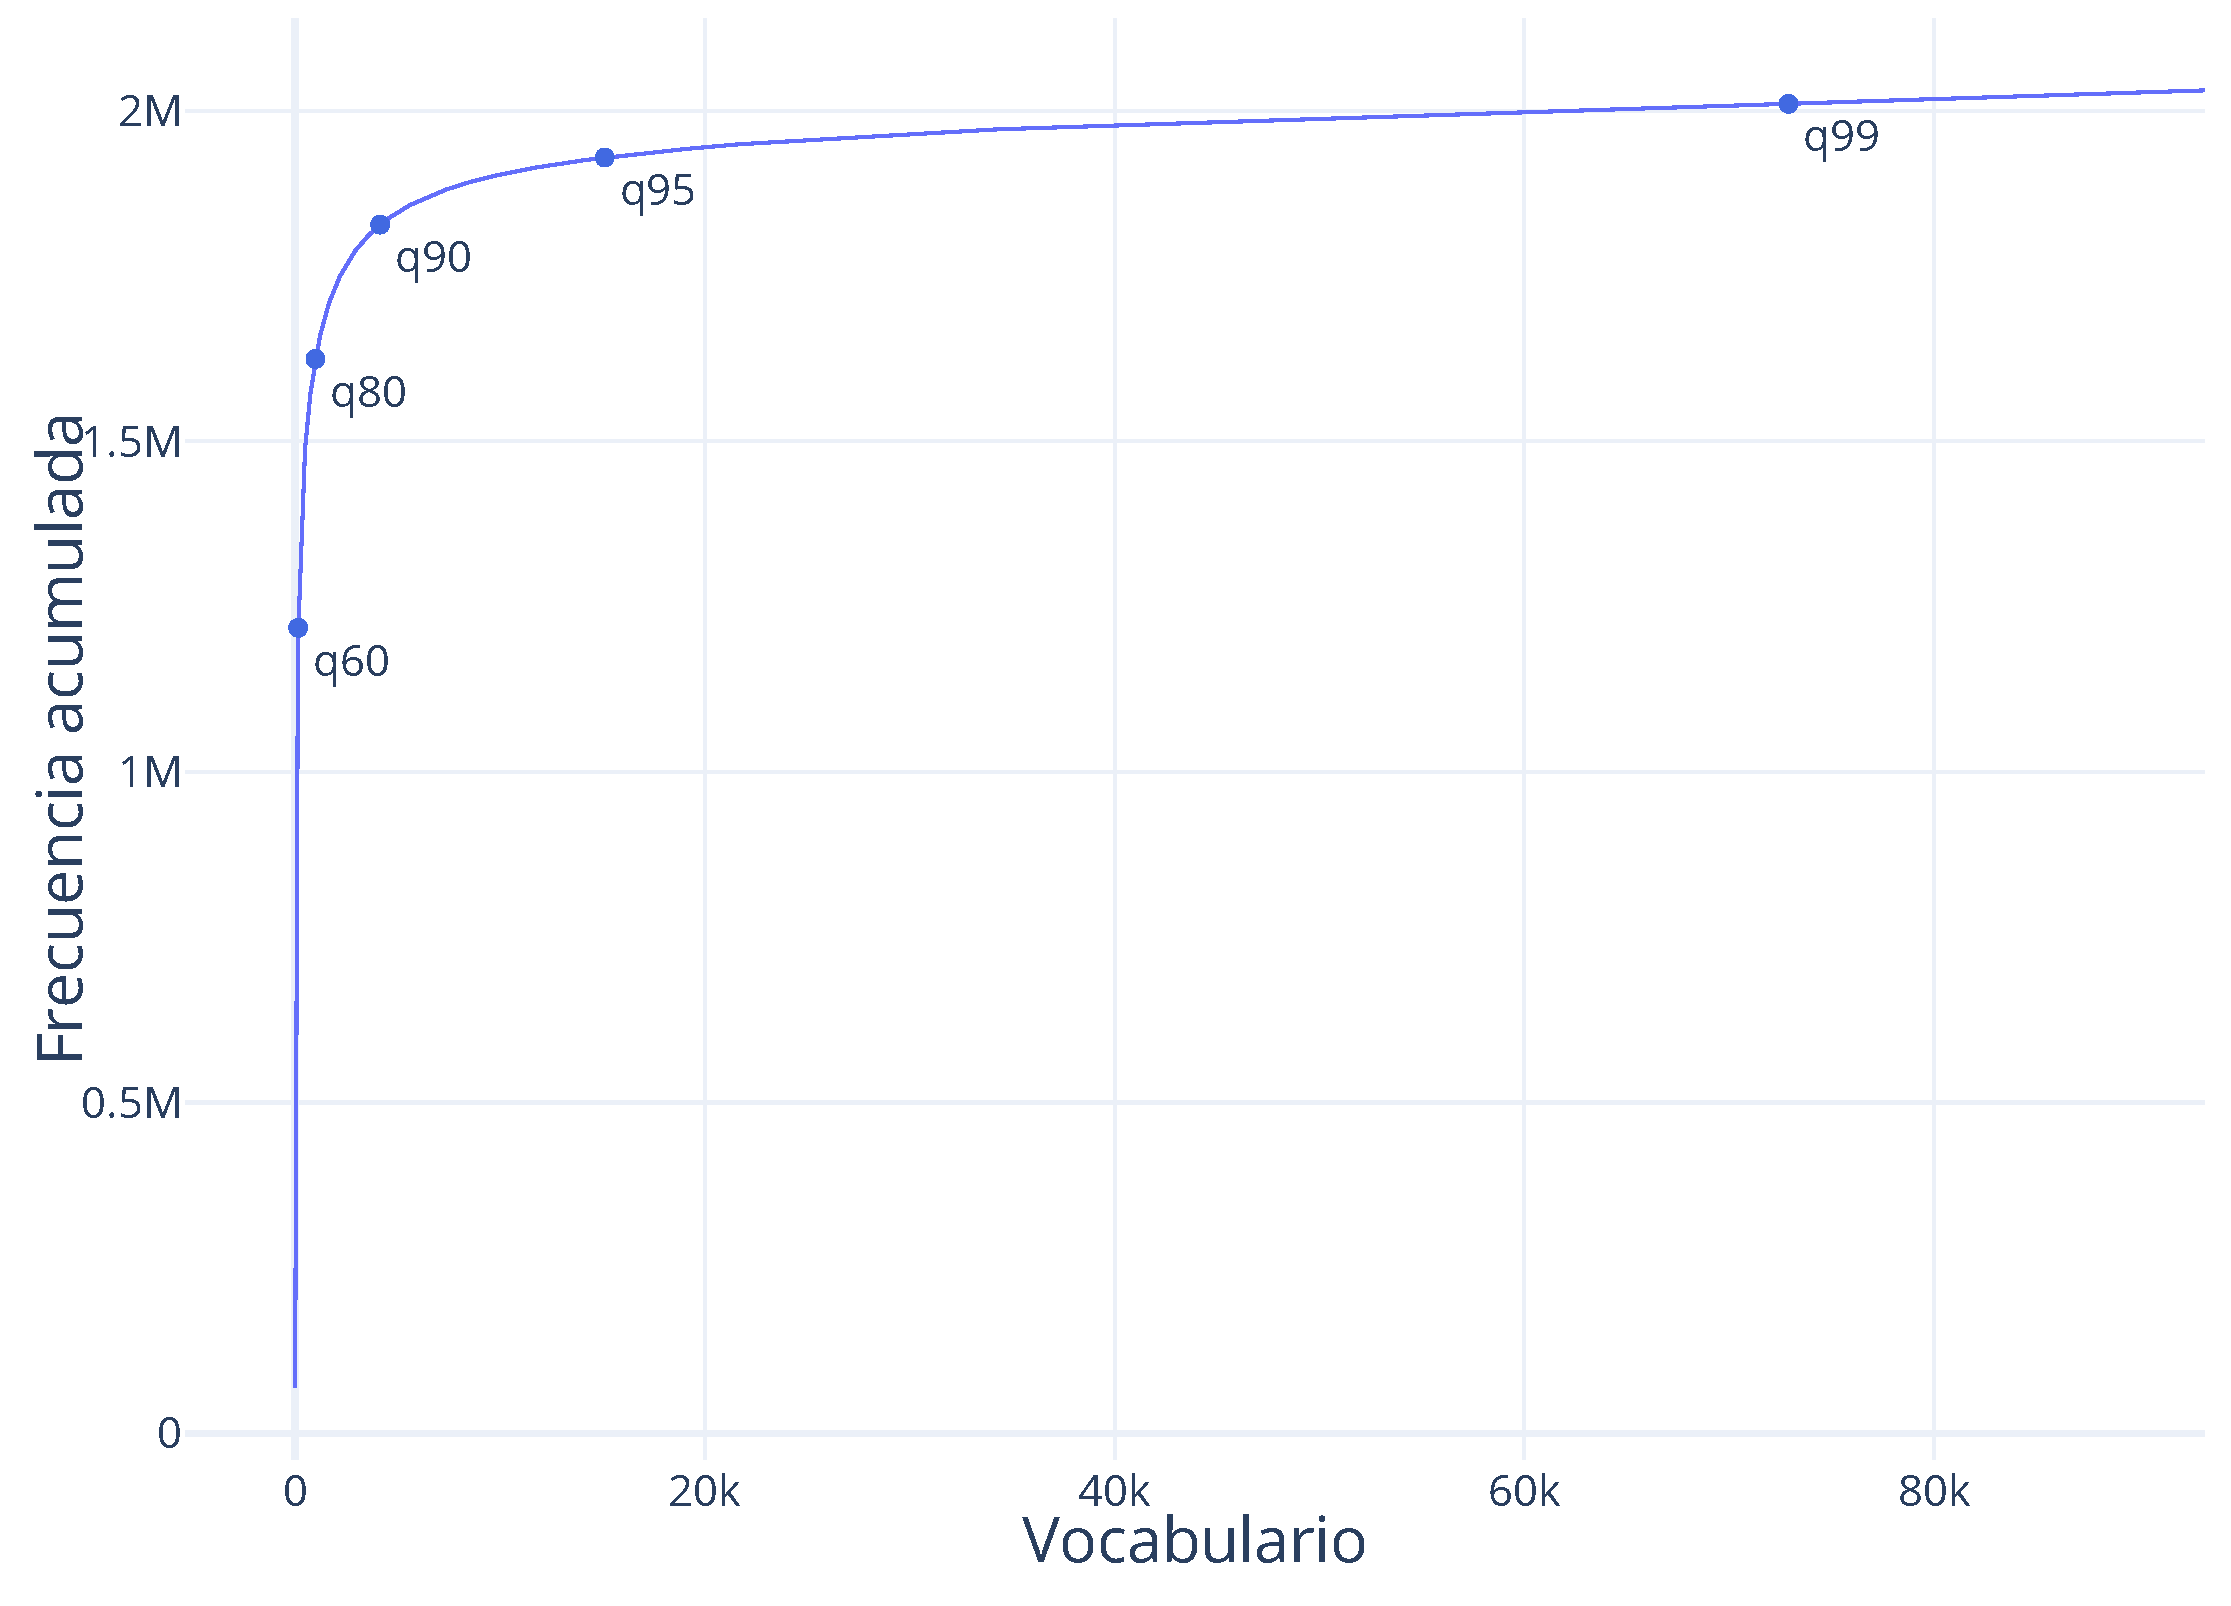
\includegraphics[trim={1.155cm 1.3cm 0 0},clip,width=0.6\textwidth]{ch4/cum_dist_1.eps}
    \caption{Frecuencia acumulada del vocabulario en orden decreciente de ocurrencia aplicando hasta el primer nivel de procesamiento.}
    \label{img:cum_dist1}
\end{figure}

En segundo lugar, se aplica la etapa de procesamiento de caracteres. De acuerdo a la Figura \ref{img:cum_dist2} el tamaño del vocabulario se reduce a casi la mitad, específicamente a 42,921 palabras, de forma similar la cantidad de \textit{tokens} se reduce a 1,028,412.

\begin{figure}
    \centering
    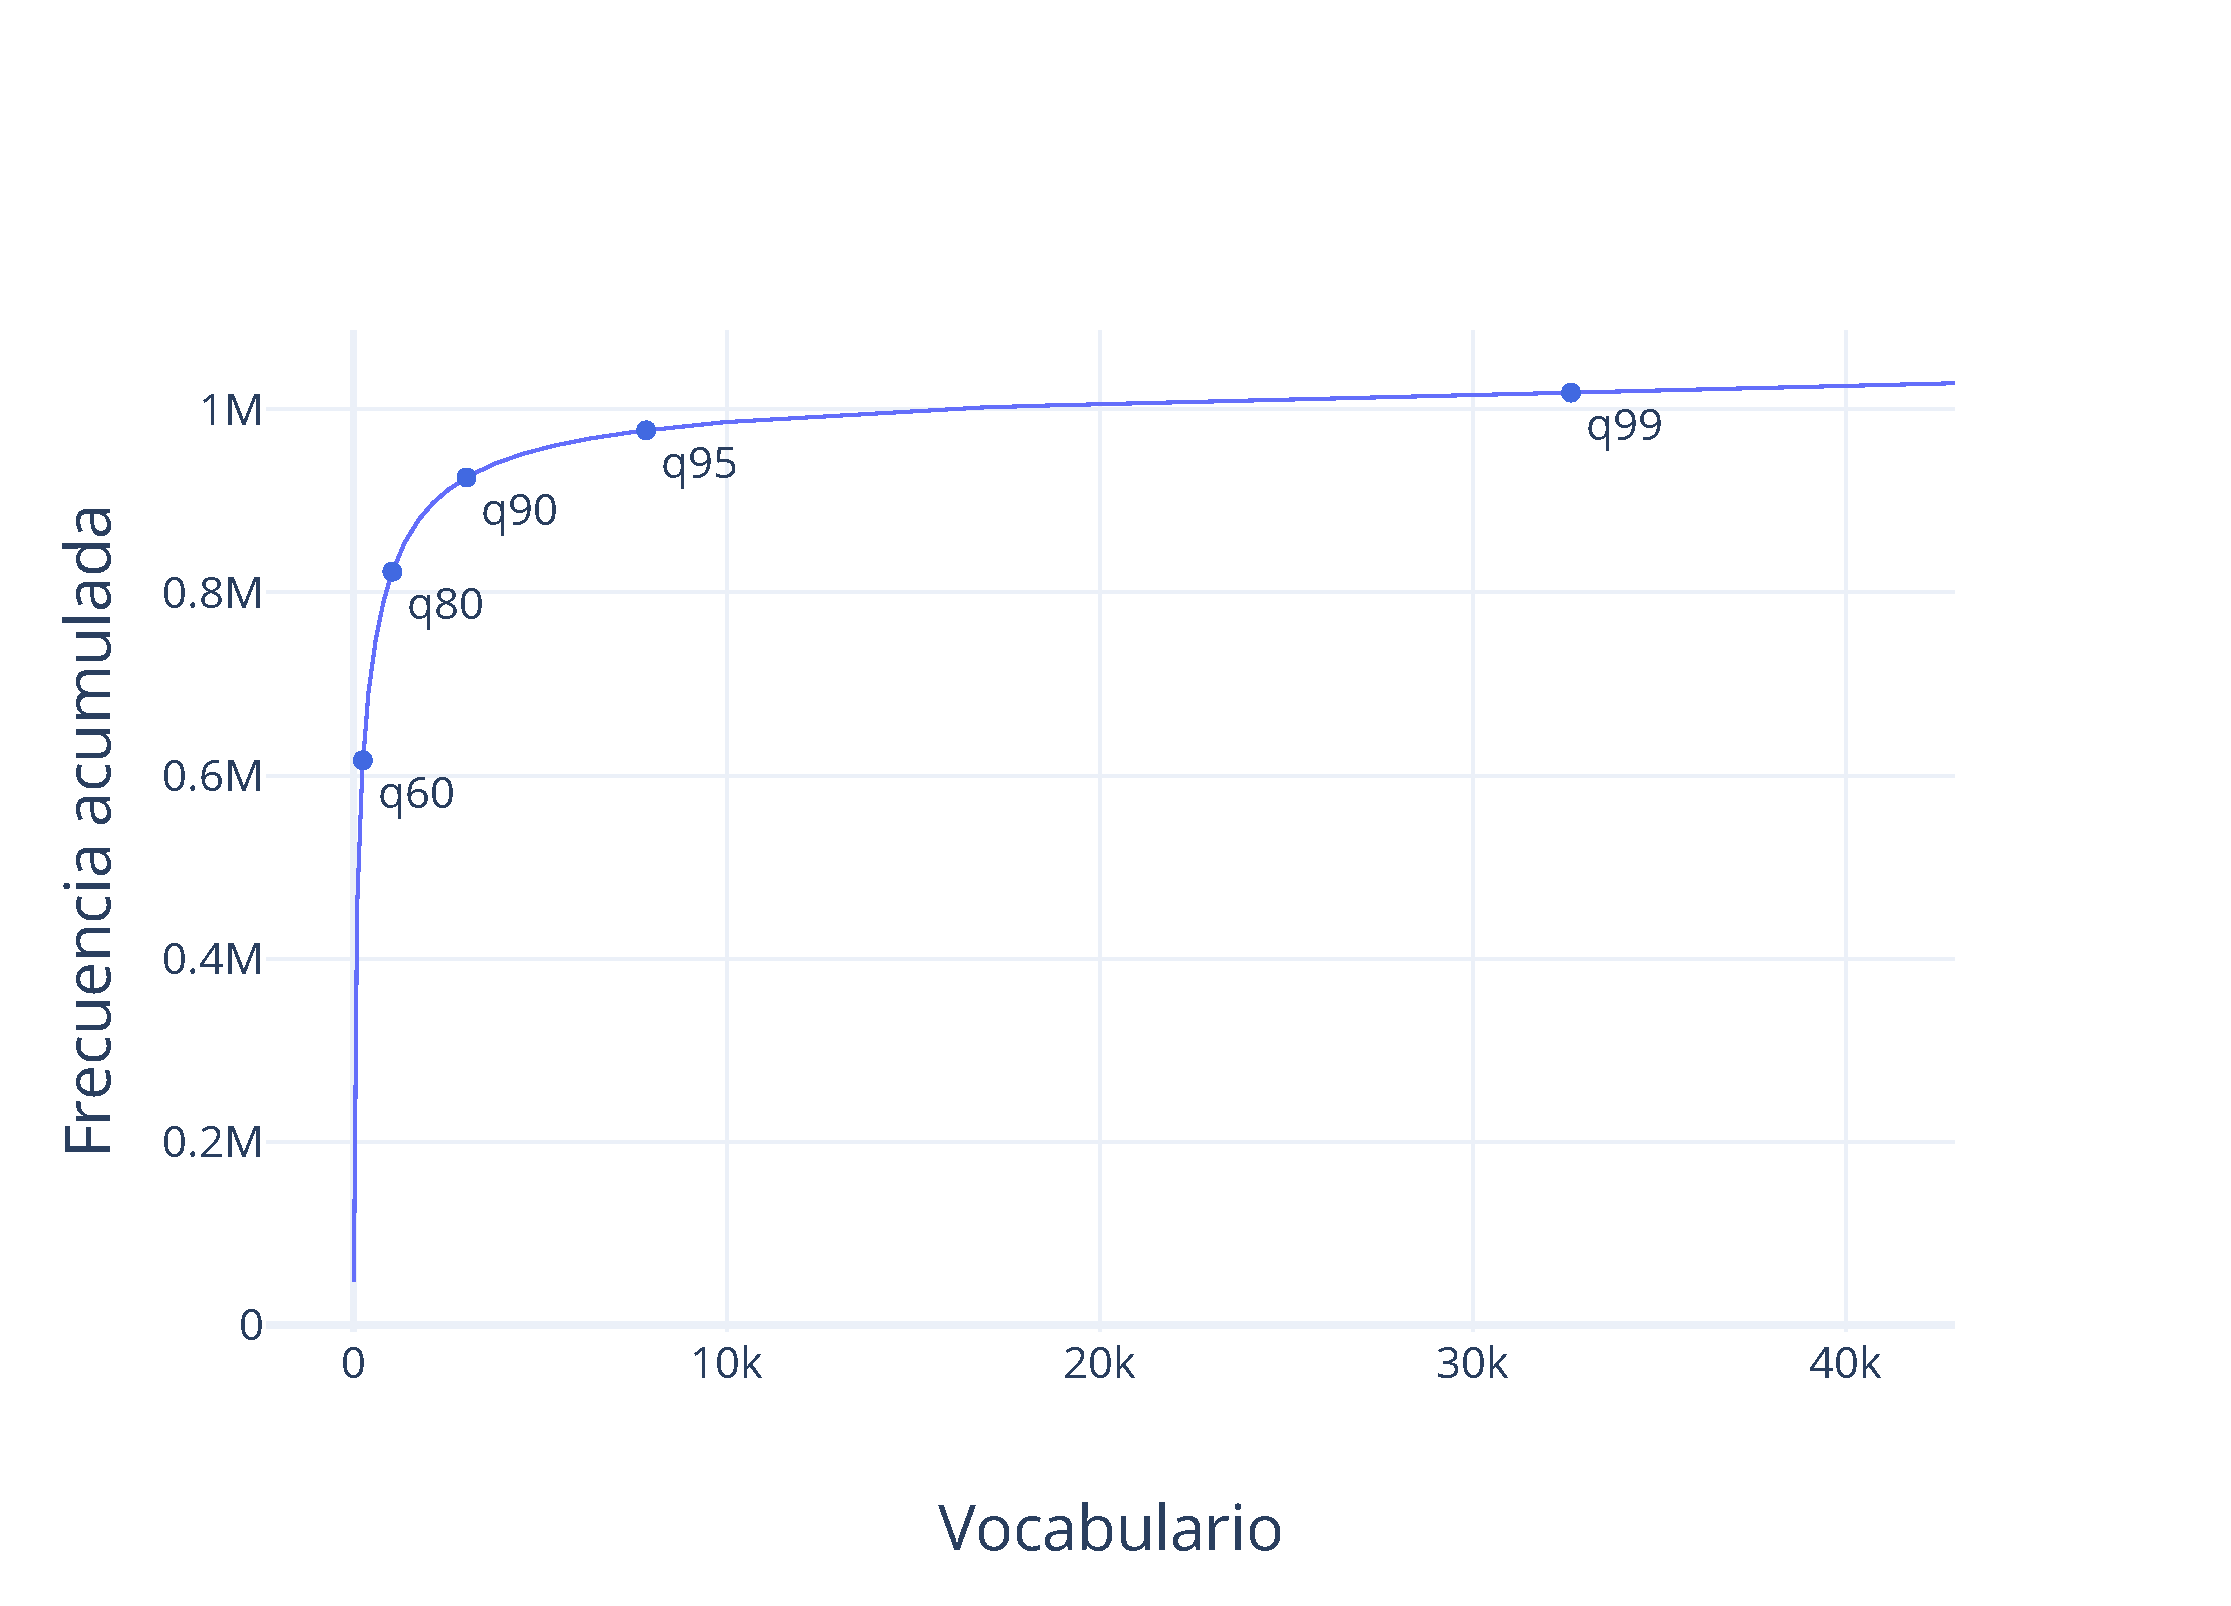
\includegraphics[trim={1.155cm 1.3cm 0 0},clip,width=0.6\textwidth]{ch4/cum_dist_2.eps}
    \caption{Frecuencia acumulada del vocabulario en orden decreciente de ocurrencia aplicando hasta el segundo nivel de procesamiento.}
    \label{img:cum_dist2}
\end{figure}

Hasta este nivel de procesamiento se tiene que cerca del 50\% de las palabras ocurren una única vez y al cerca de un 80\% tiene una frecuencia igual o menor a 4. El 95\% de la distribución acumulada puede ser explicada con 7,837 palabras (un 18\% del vocabulario actual). En conclusión, la distribución de las palabras tiene una cola bastante pesada.\\

En tercer lugar, se eliminan las palabras que aparecen en menos del 0.1\% de los documentos de su época. En la Figura \ref{img:cum_dist3} se muestra una reducción importante del vocabulario, específicamente a 3,148 (al rededor de 14 veces), reduciendo levemente  (alrededor de un 10\%) la cantidad de \textit{tokens} a 925,693.\\

\begin{figure}
    \centering
    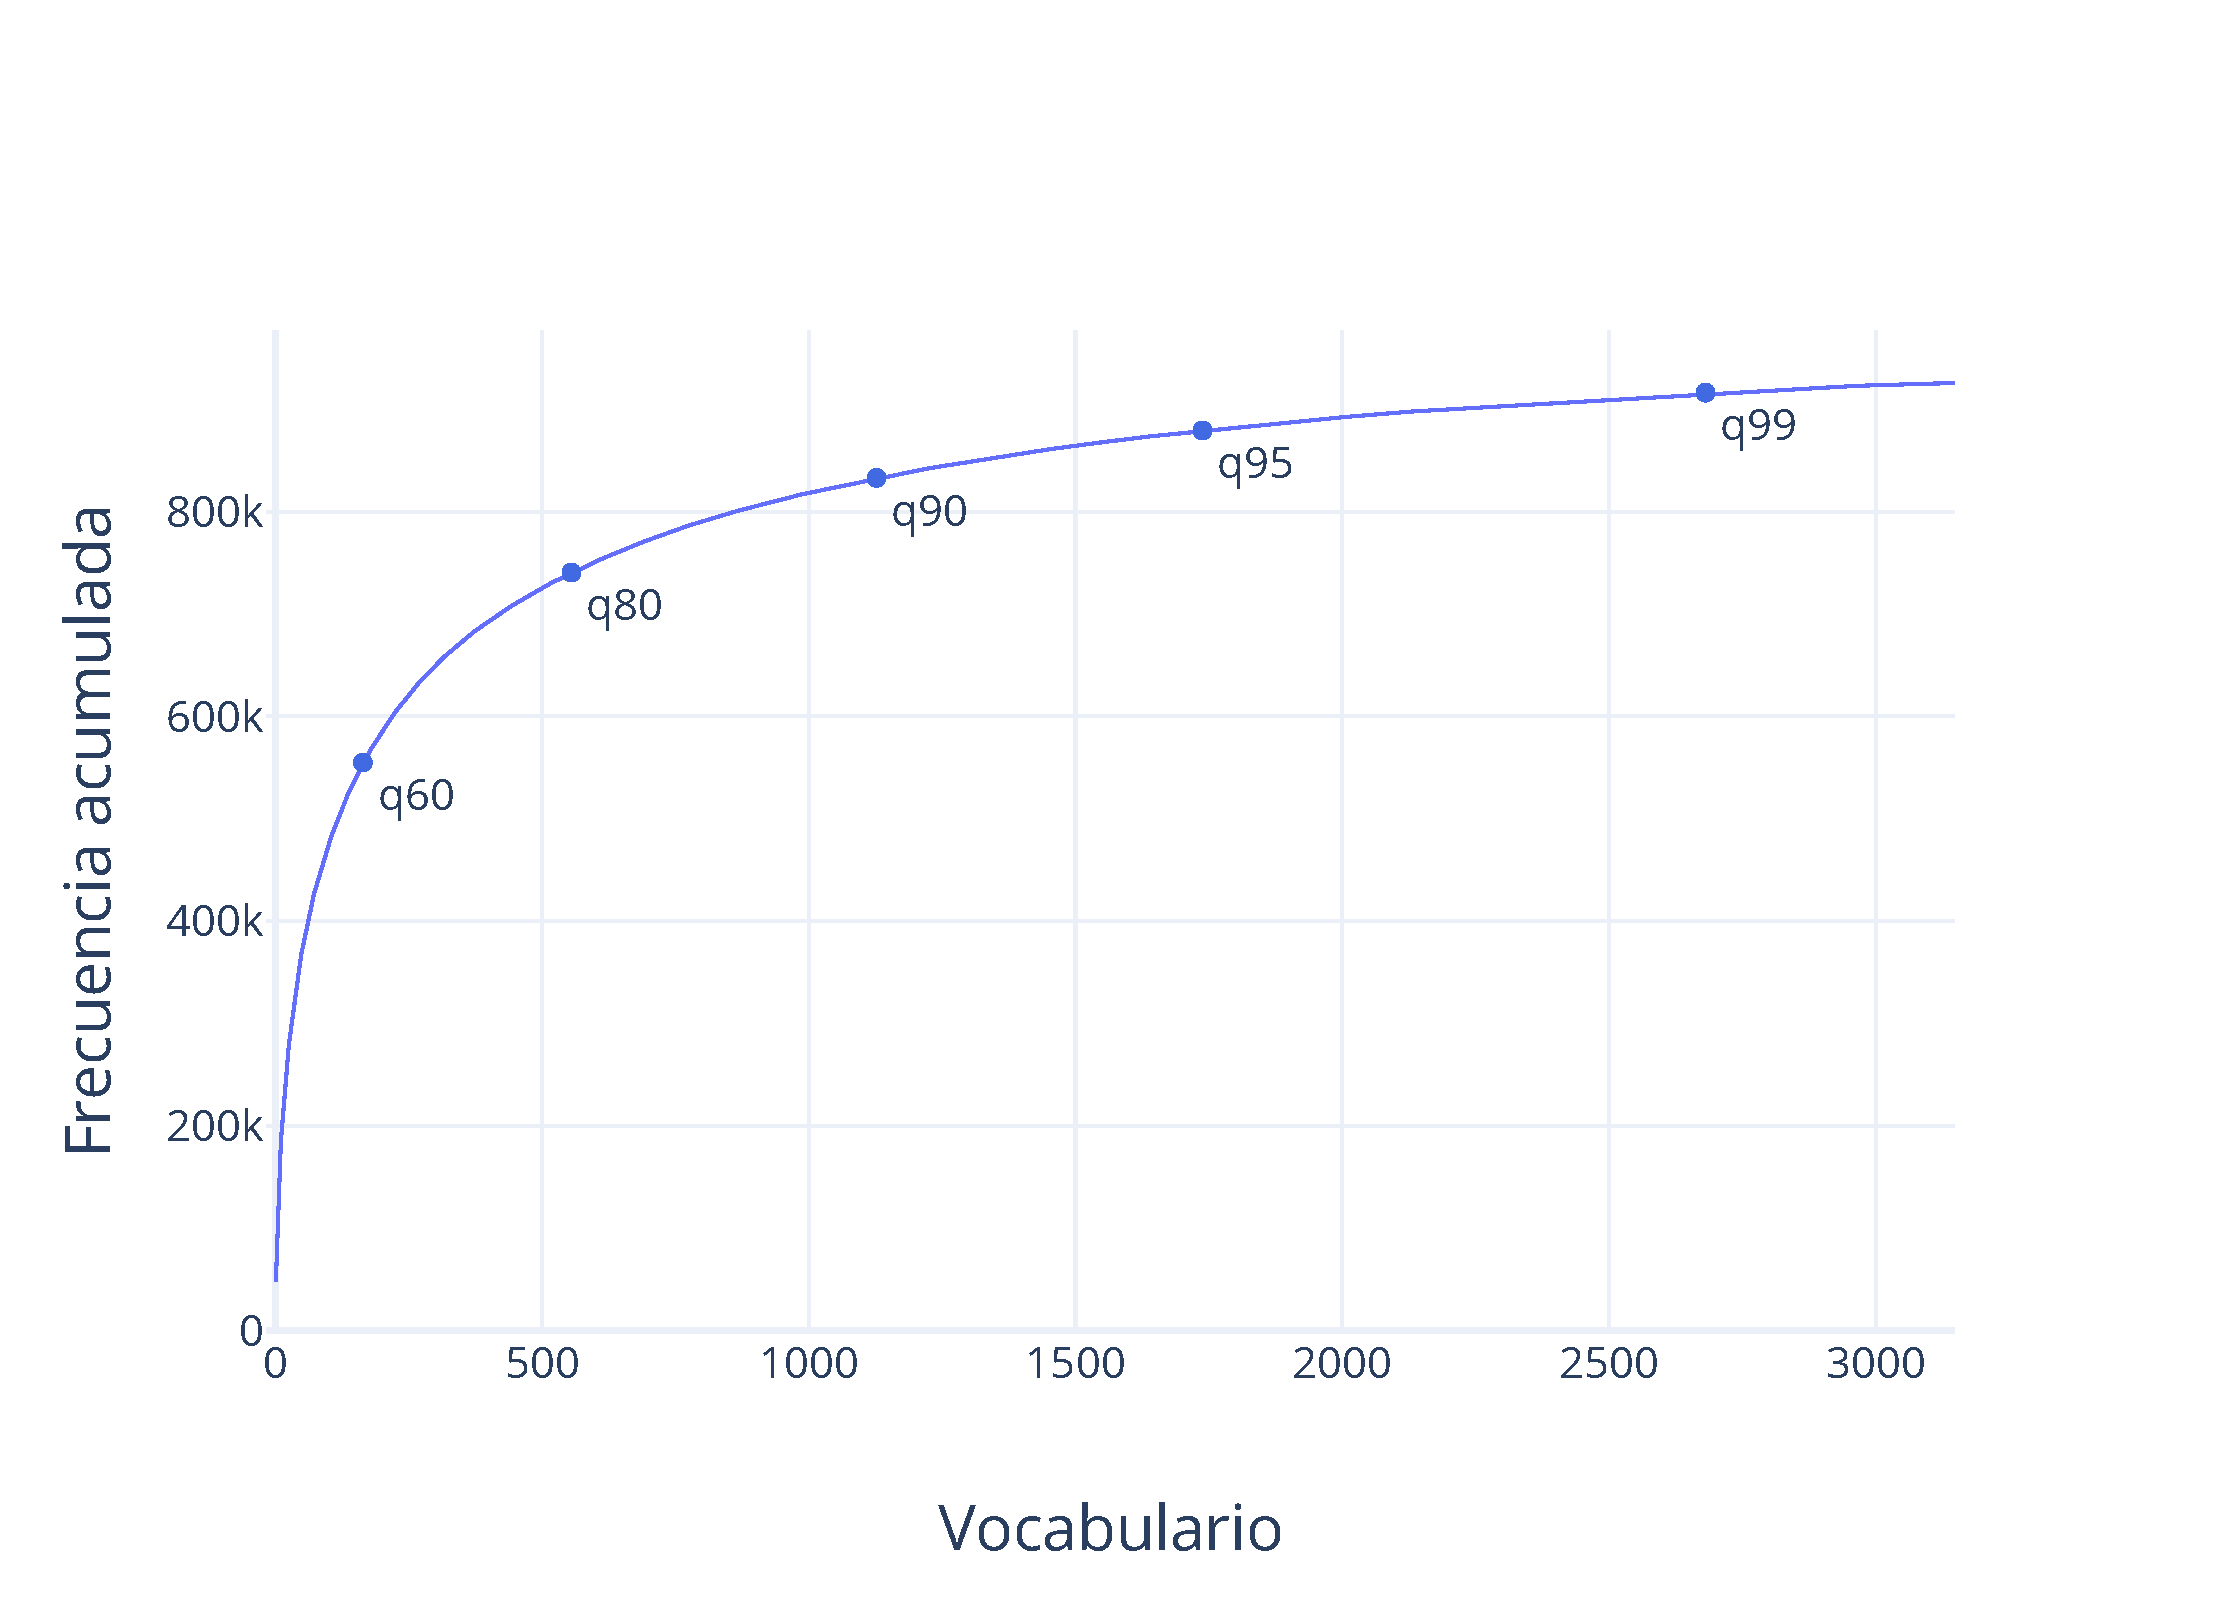
\includegraphics[trim={1.155cm 1.3cm 0 0},clip,width=0.6\textwidth]{ch4/cum_dist_3.eps}
    \caption{Frecuencia acumulada del vocabulario en orden decreciente de ocurrencia aplicando hasta el tercer nivel de procesamiento.}
    \label{img:cum_dist3}
\end{figure}

En cuarto lugar, se filtran palabras usando el vocabulario extraído del SUC. En la Figura \ref{img:cum_dist4} se observa que el vocabulario se redujo a 2,902 y el la cantidad de \textit{tokens} a 901,745. En este caso la variación no fue menos significativa, alrededor de un 8\% en el tamaño del vocabulario y de un 3\% en el caso de los \textit{tokens}.\\

\begin{figure}
    \centering
    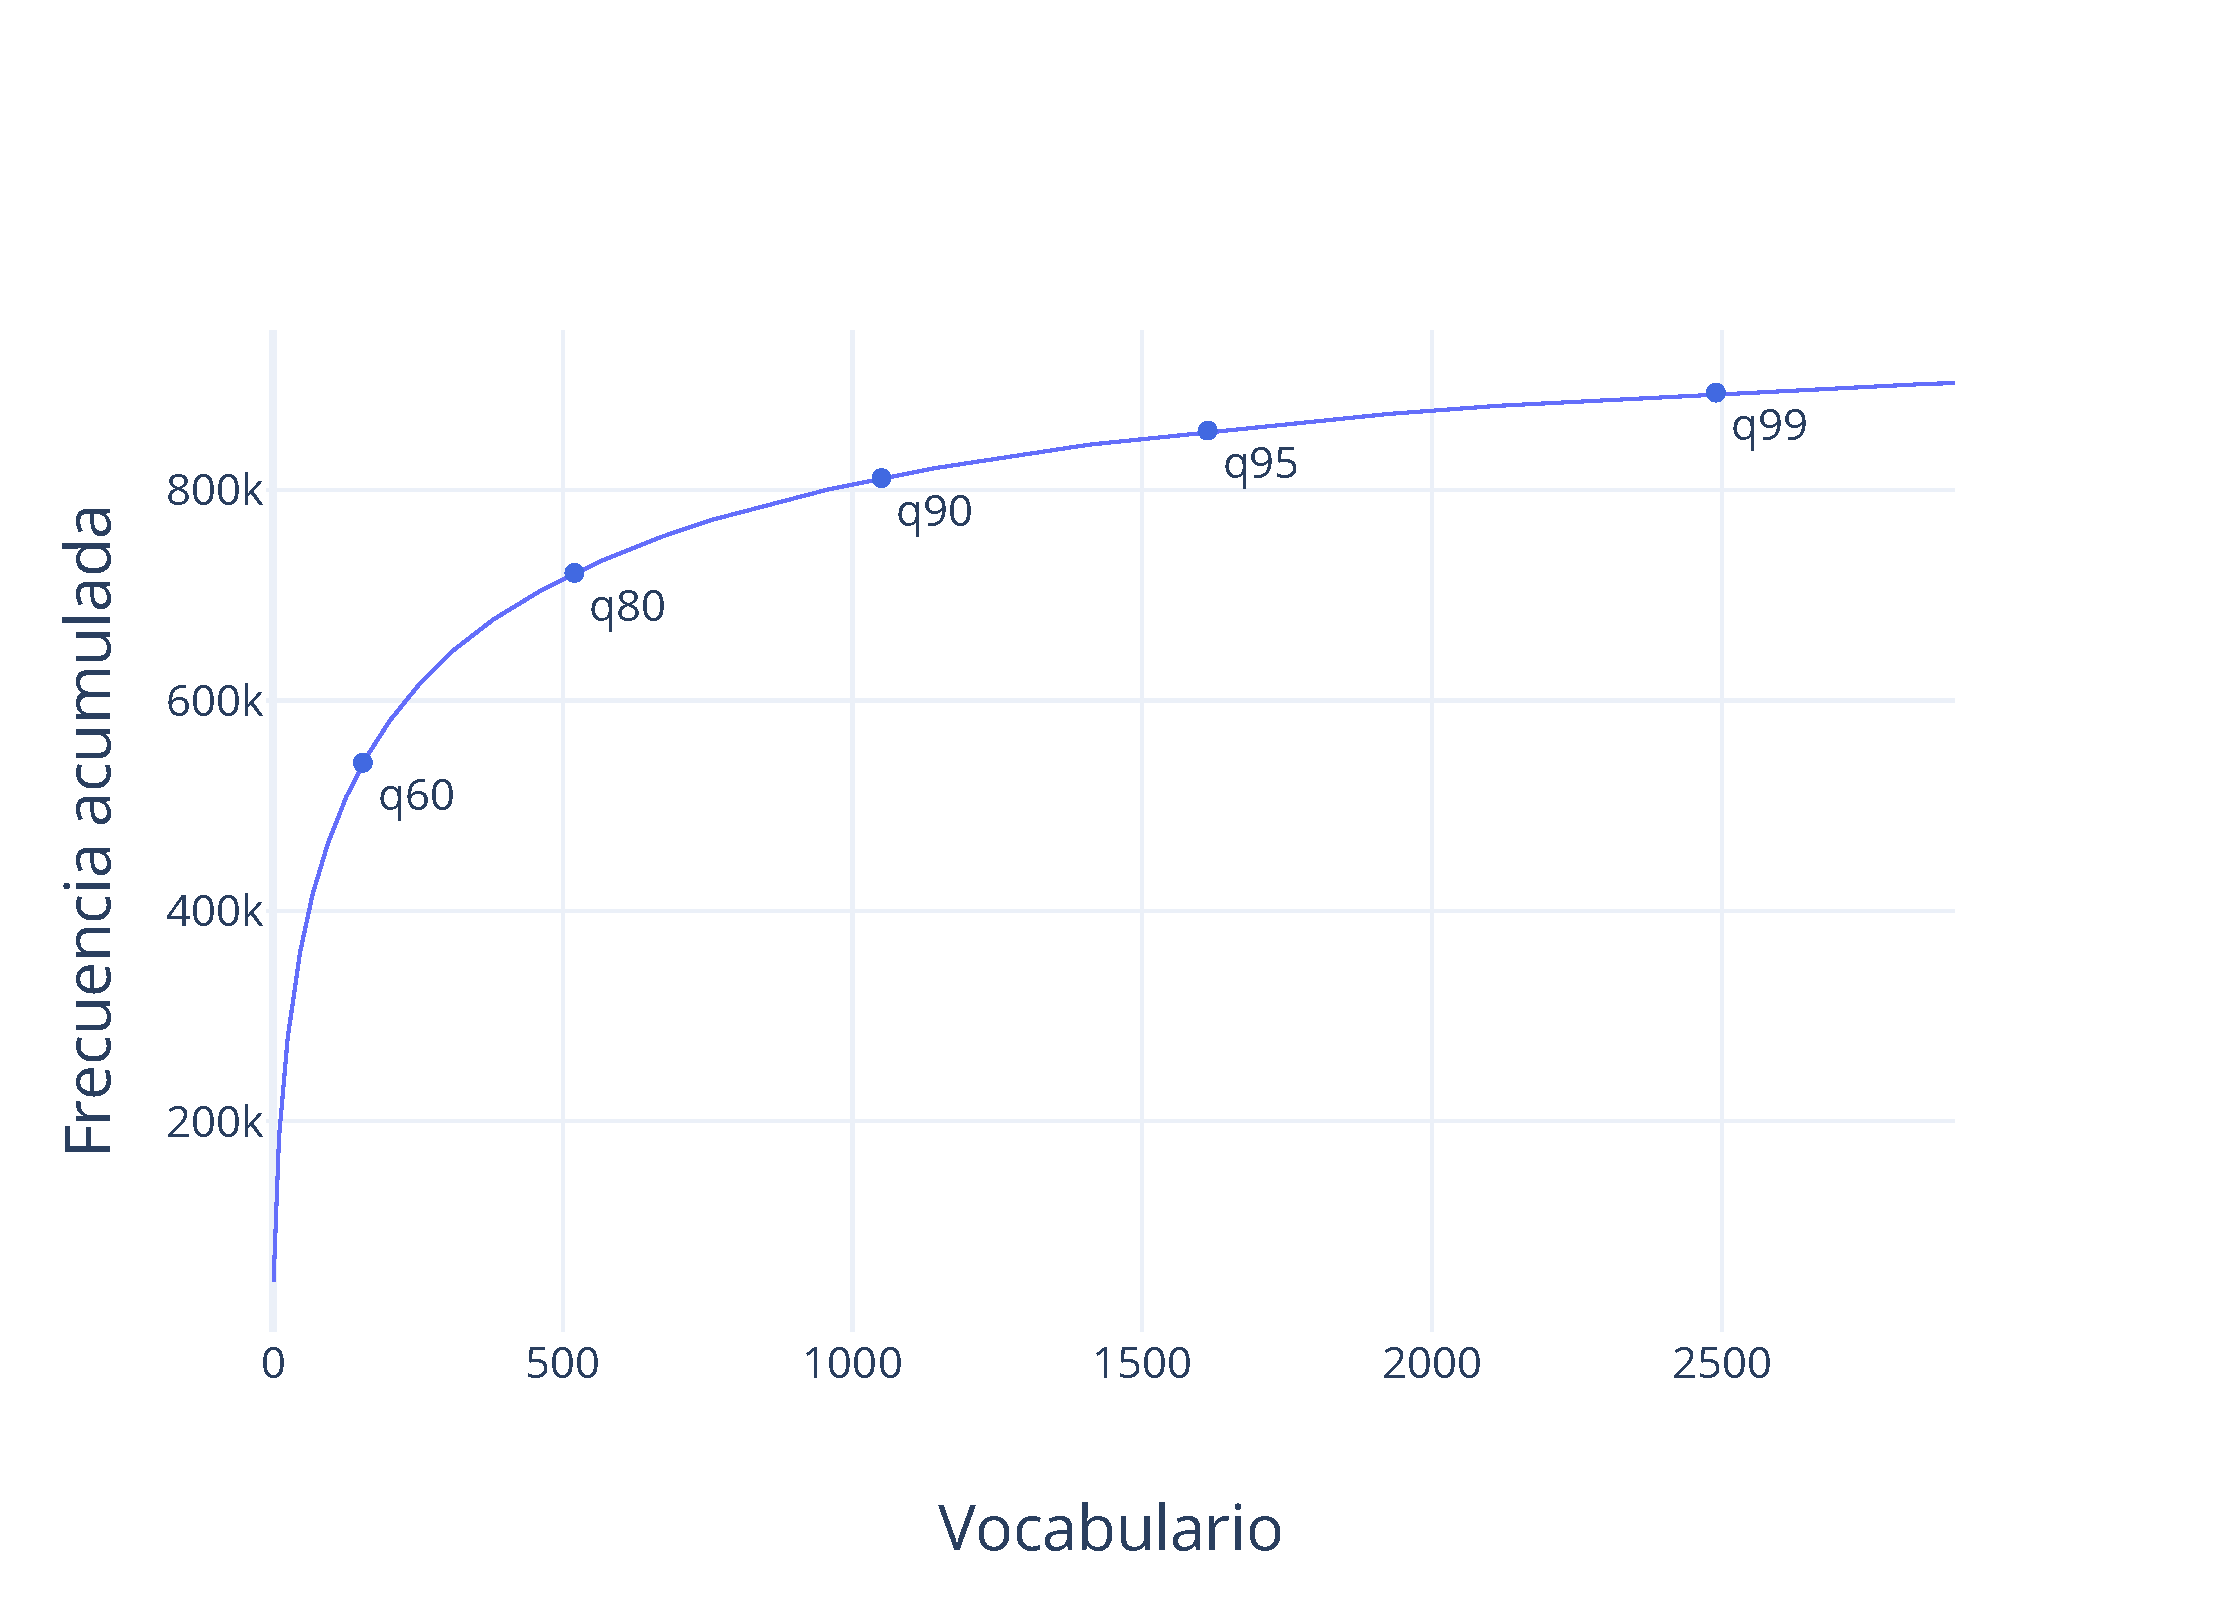
\includegraphics[trim={1.155cm 1.3cm 0 0},clip,width=0.6\textwidth]{ch4/cum_dist_4.eps}
    \caption{Frecuencia acumulada del vocabulario en orden decreciente de ocurrencia aplicando hasta el cuarto nivel de procesamiento.}
    \label{img:cum_dist4}
\end{figure}

En quinto lugar, se eliminan las \textit{stopwords}, de la Figura \ref{img:cum_dist5} se puede observar que significó una reducción significativa de tanto el vocabulario como del número de \textit{tokens}, respectivamente en 32\% (1,960 palabras) y 45\% (495,182 \textit{tokens}). La reducción abrupta en la cantidad de \textit{tokens} se debe principalmente a que las \textit{stopwords} son parte de las palabras más frecuentes dentro del corpus.\\

\begin{figure}
    \centering
    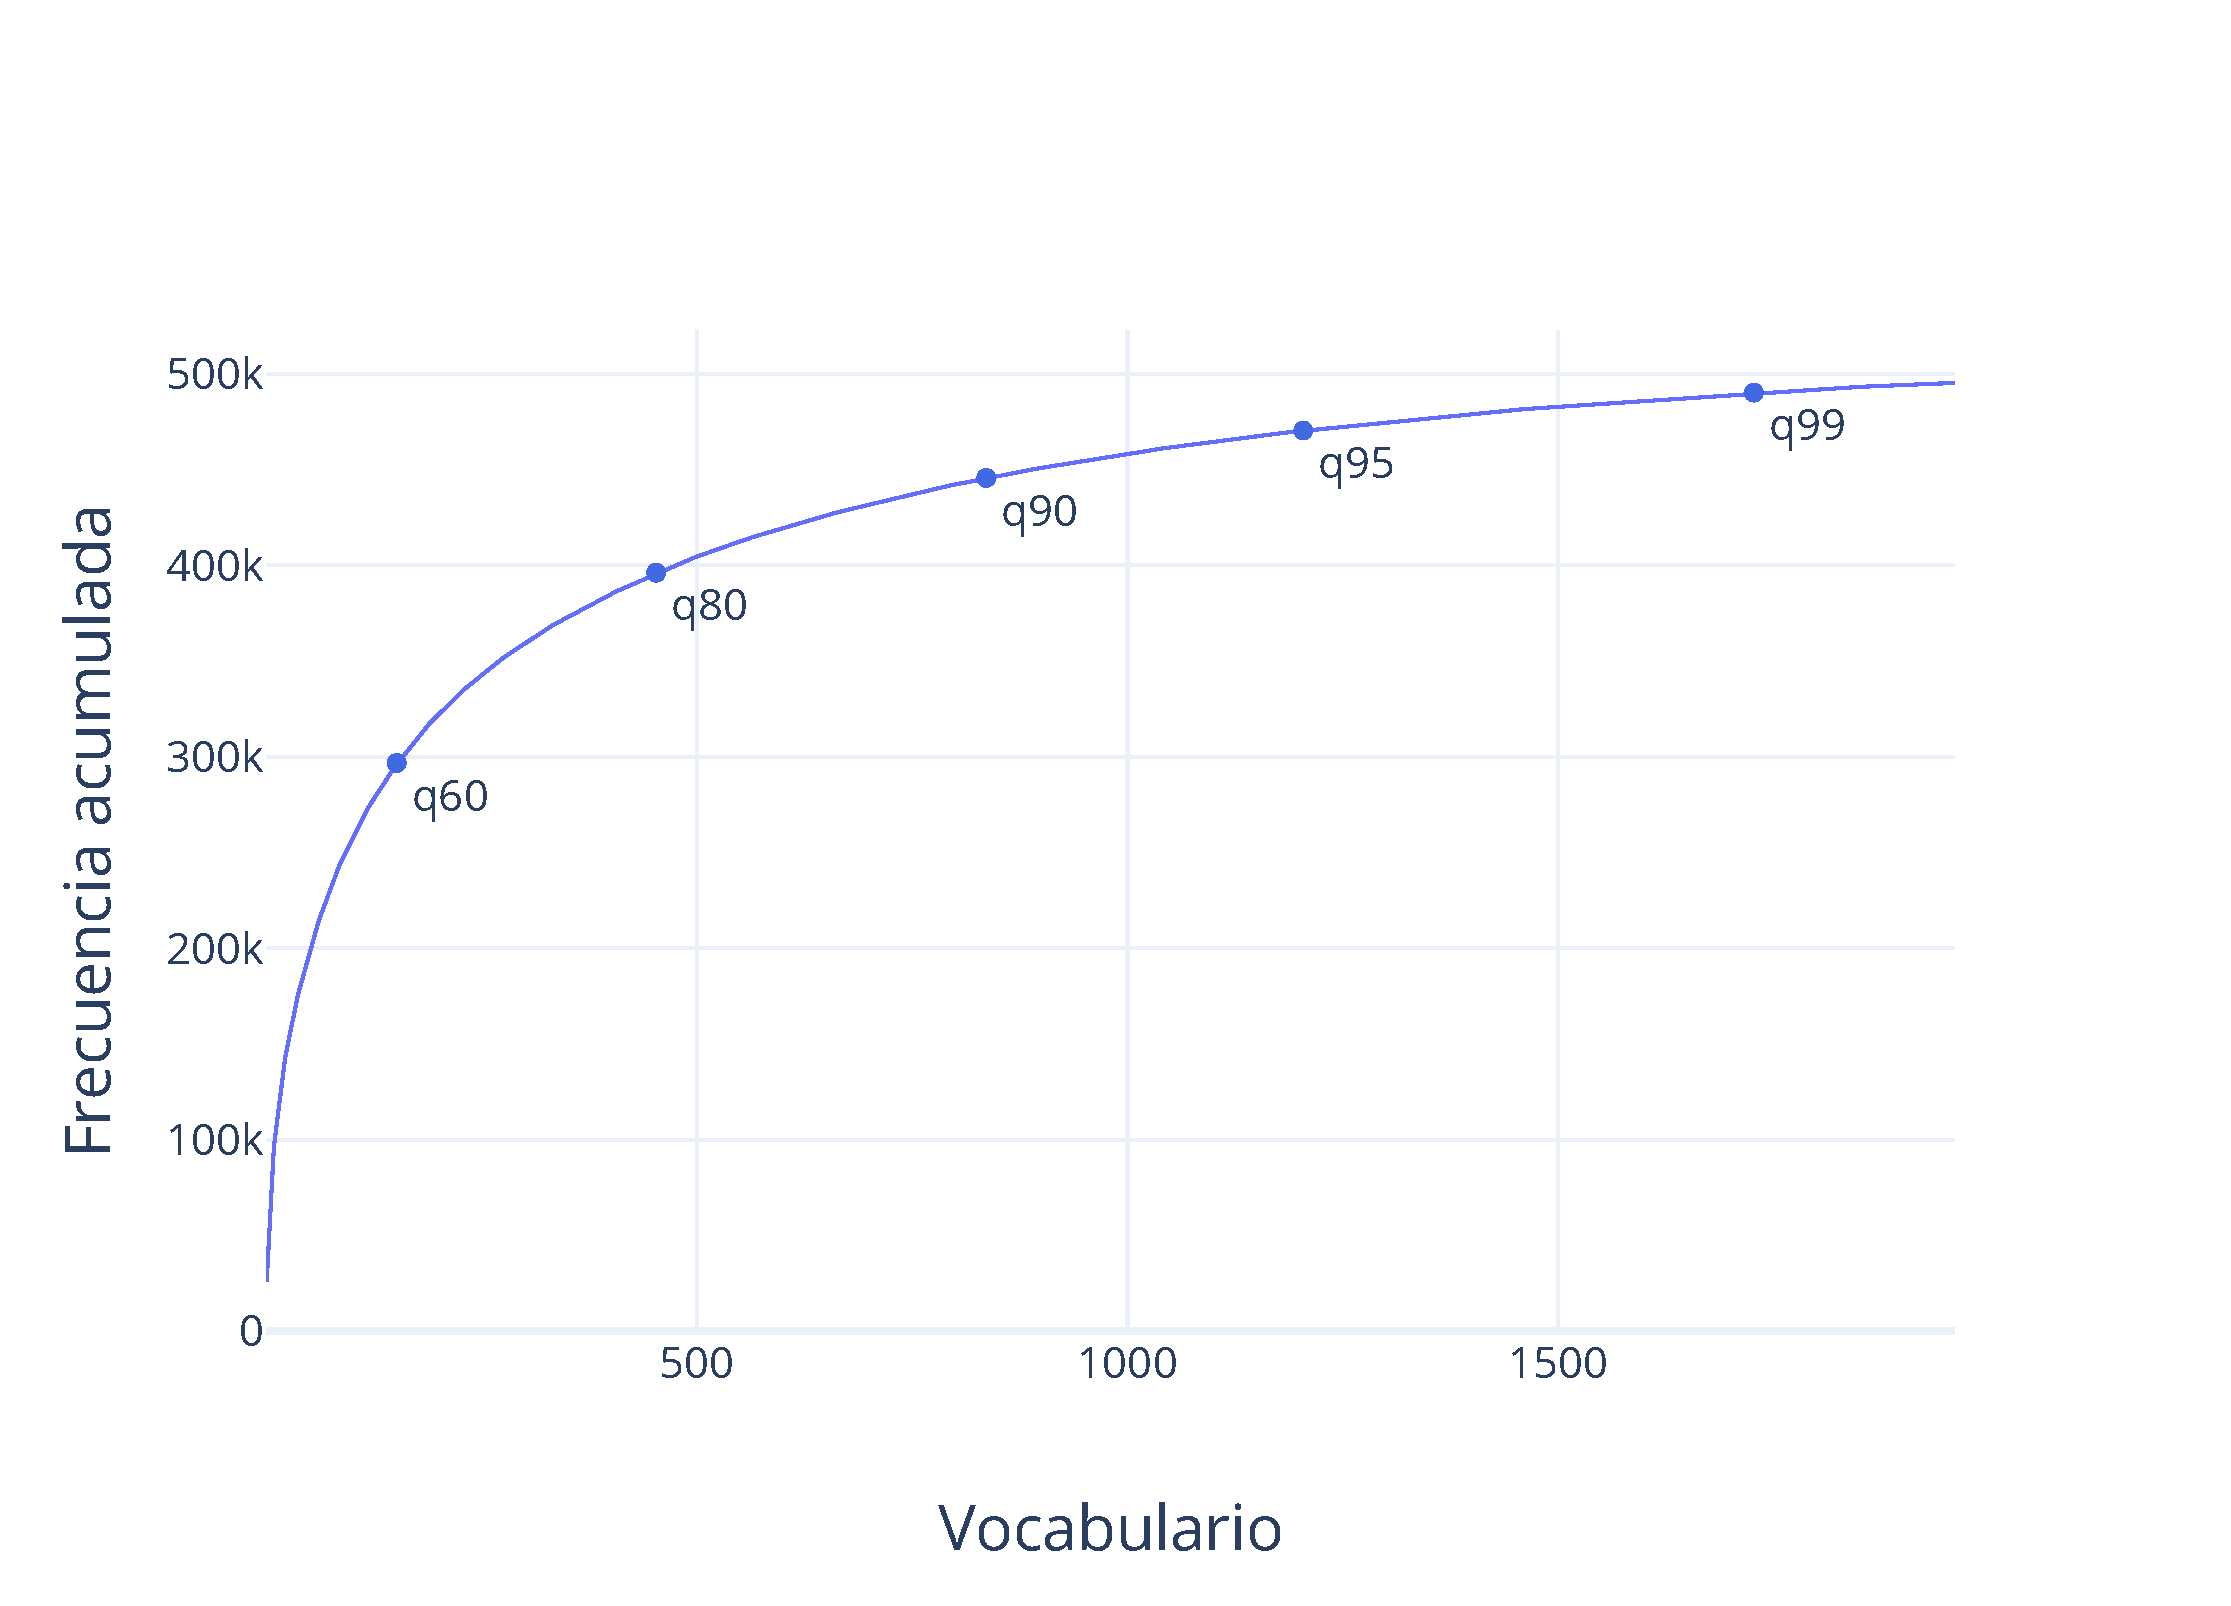
\includegraphics[trim={1.155cm 1.3cm 0 0},clip,width=0.6\textwidth]{ch4/cum_dist_5.eps}
    \caption{Frecuencia acumulada del vocabulario en orden decreciente de ocurrencia aplicando hasta el quinto nivel de procesamiento.}
    \label{img:cum_dist5}
\end{figure}

Por último, se eliminan los documentos con menos de 5 palabras, de la Figura \ref{img:cum_dist6} se puede observar que implicó una reducción de alrededor del 20\% en el tamaño del corpus y del 8\% en el número de \textit{tokens}.

\begin{figure}
    \centering
    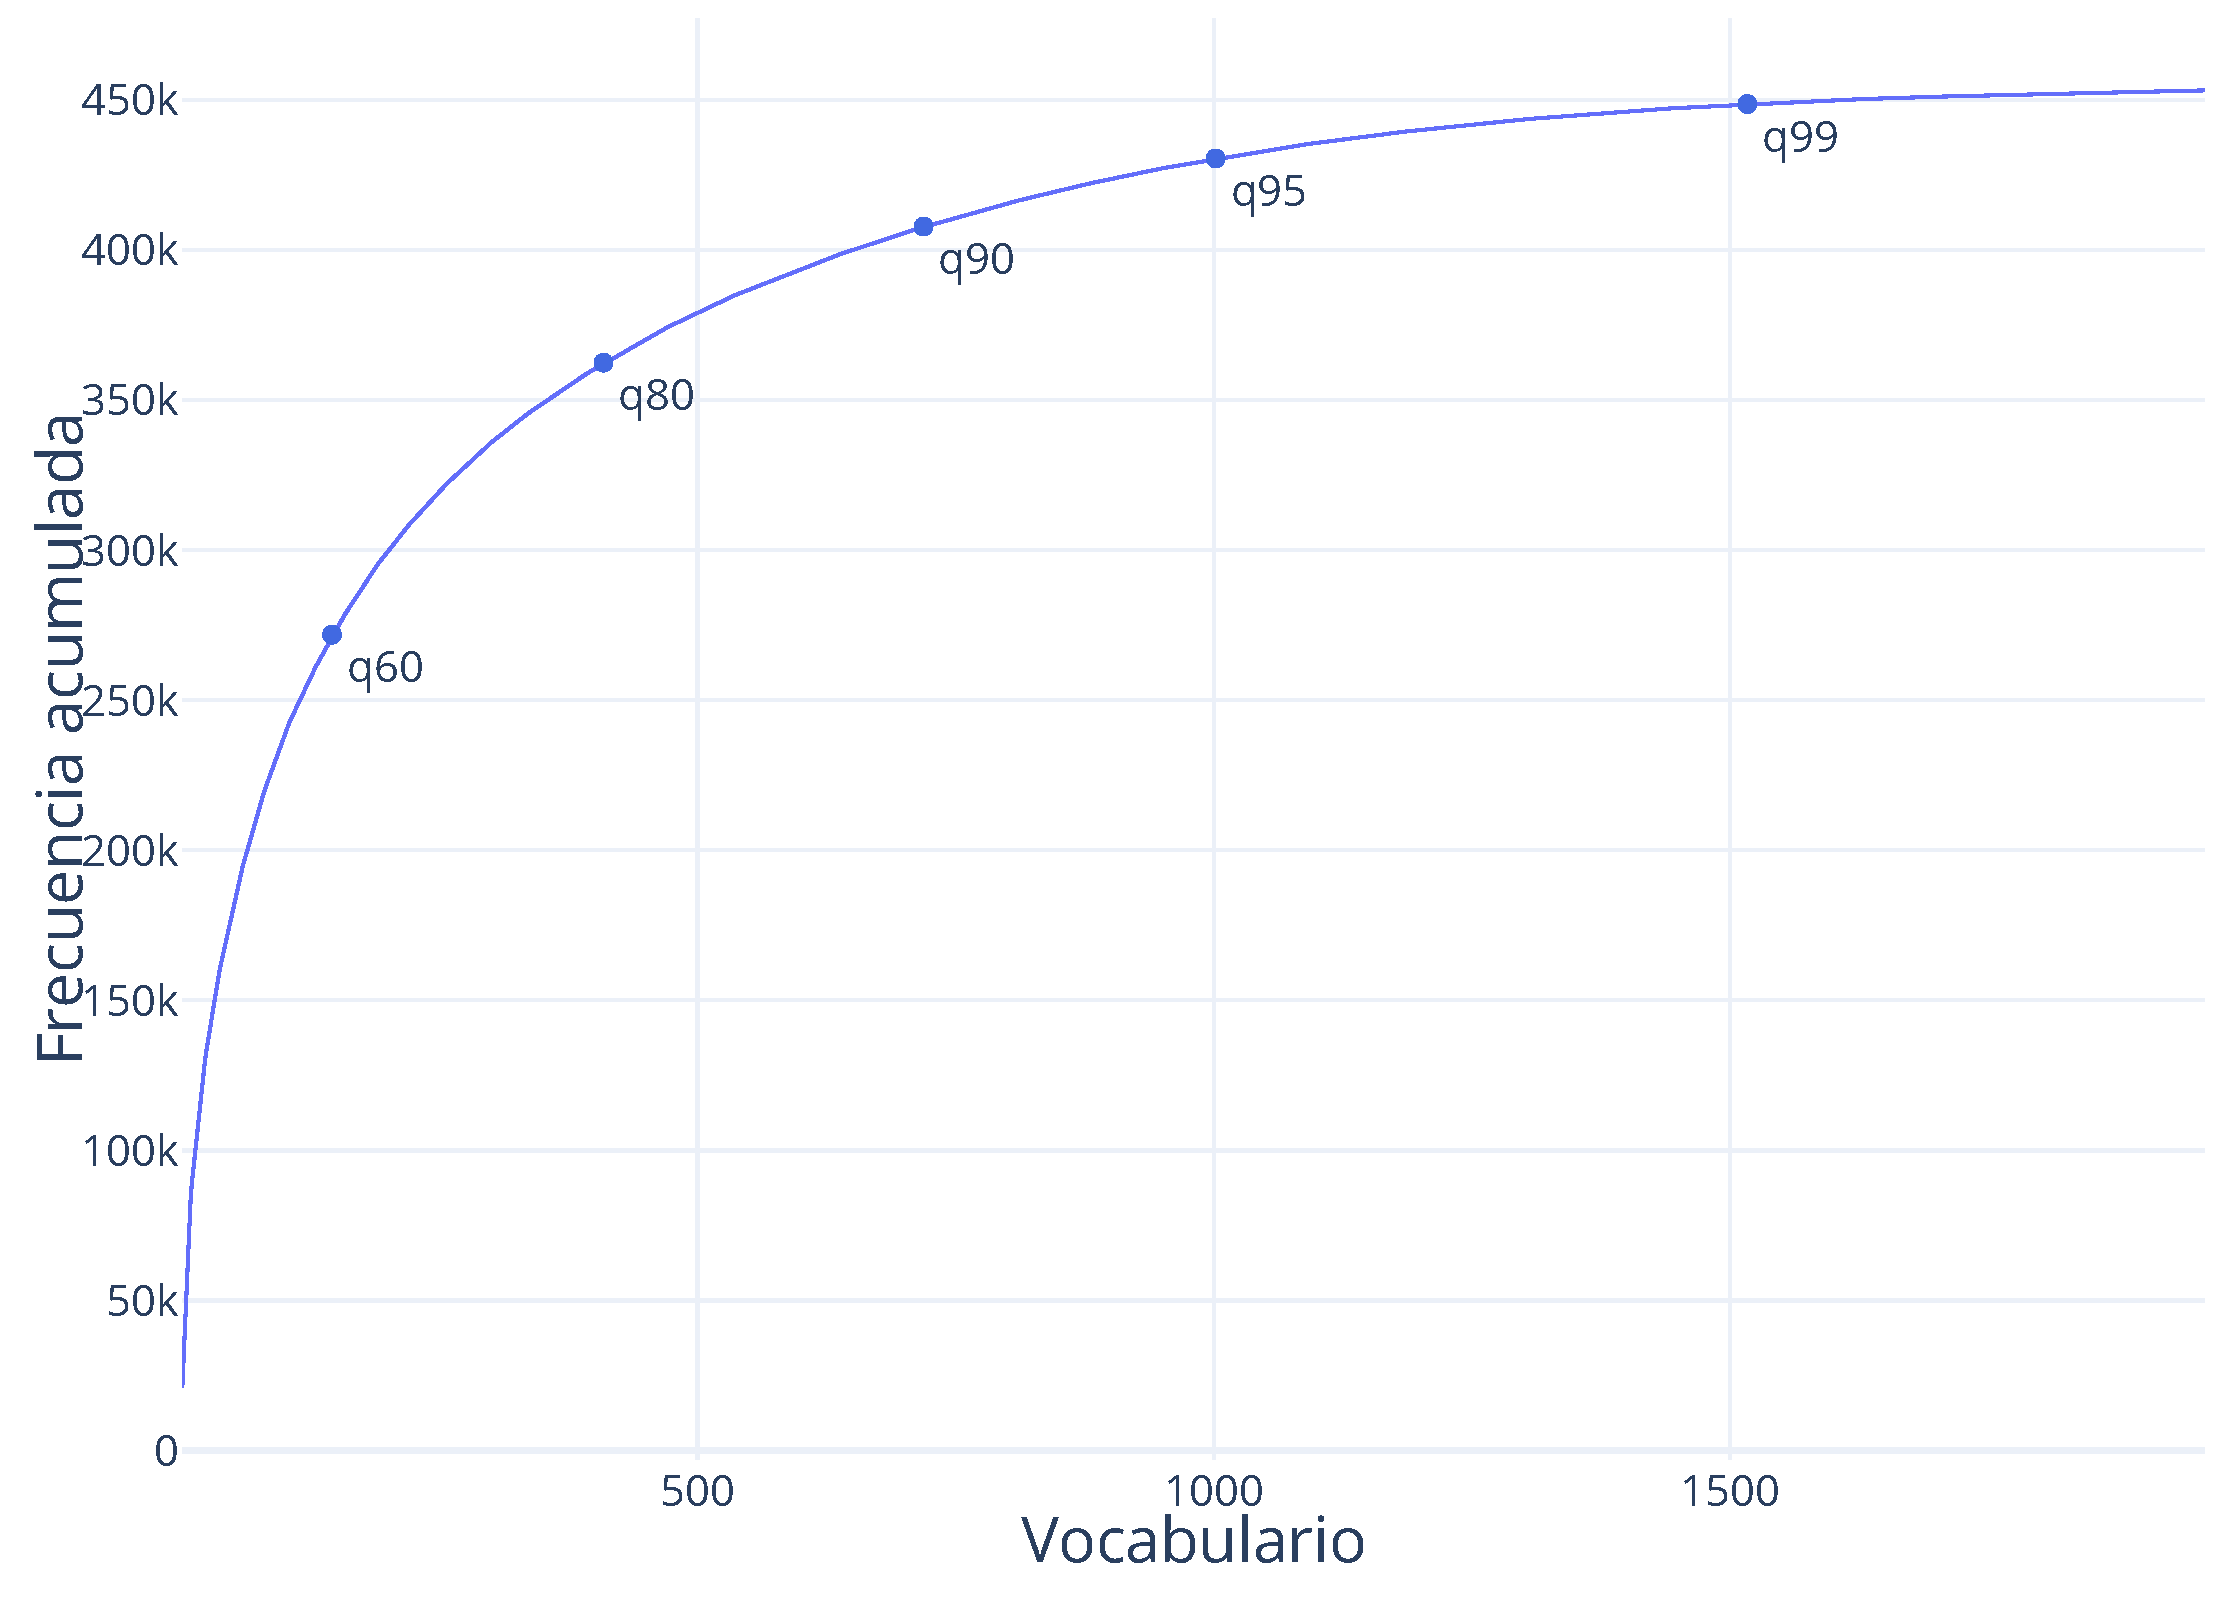
\includegraphics[trim={1.155cm 1.3cm 0 0},clip,width=0.6\textwidth]{ch4/cum_dist_6.eps}
    \caption{Frecuencia acumulada del vocabulario en orden decreciente de ocurrencia aplicando hasta el sexto nivel de procesamiento.}
    \label{img:cum_dist6}
\end{figure}

En la tabla \ref{table:processing_stats} se muestra un cuadro resumen con estadísticas del corpus bajo distintos niveles de procesamiento. De aquí se extrae que el tamaño del vocabulario, el corpus y la cantidad de \textit{tokens} se redujo en alrededor de un 98\%, un 20\% y un 76\% respectivamente.

\begin{table}[H]
    \begin{tabular}{|c|c|c|c|}
    \hline
    procesamiento & documentos & vocabulario & tokens  \\ \hline
    t             & 49,015      & 93,203       & 2,030,980 \\ \hline
    t+ch          & 49,003      & 42,921       & 1,028,412 \\ \hline
    t+ch+f        & 48,988      & 3,148        & 925,693  \\ \hline
    t+ch+f+v      & 48,988      & 2,902        & 901,745  \\ \hline
    t+ch+f+v+s    & 48,566      & 1,960        & 495,182  \\ \hline
    t+ch+f+v+s+d  & 38,850      & 1,960        & 453,206  \\ \hline
    \end{tabular}
    \caption{Estadísticas del corpus bajo distintos niveles de procesamientos, \textbf{t}: tokenización, \textbf{ch}: procesamiento de caracteres, \textbf{f}: filtro por frecuencia, \textbf{v}: filtro por vocabulario, \textbf{s}: eliminación de \textit{stopwords}, \textbf{d}: eliminación de documentos.}
    \label{table:processing_stats}
    \end{table}

En la tabla \ref{table:innovation_rate} se muestra el detalle del vocabulario para cada una de las épocas tras procesar el corpus, de aquí se extrae que en promedio un 12.83\% del vocabulario se olvida de una época a otra y un 18.92\% es nuevo, en otras palabras, en promedio alrededor de un 32\% del vocabulario no es común entre tópicos de épocas adyacentes. Esto justifica la necesidad de utilizar medidas de similitud robustas a cambios en el vocabulario, permitiendo así una comparación más justa entre tópicos sin vocabulario común.

\begin{table}[H]
    \begin{tabular}{|c|r|r|r|r|}
    \hline
    \textbf{época} & \multicolumn{1}{c|}{\textbf{t-1}} & \multicolumn{1}{c|}{\textbf{t}} & \multicolumn{1}{c|}{\textbf{t-1 {[}\%{]}}} & \multicolumn{1}{l|}{\textbf{t {[}\%{]}}} \\ \hline
    2              & 1,145                              & 1,187                            & 14.41                                      & 18.08                                    \\ \hline
    3              & 1,187                              & 1,281                            & 13.56                                      & 21.48                                    \\ \hline
    4              & 1,281                              & 1,329                            & 13.35                                      & 17.10                                    \\ \hline
    5              & 1,329                              & 1,405                            & 12.57                                      & 18.28                                    \\ \hline
    6              & 1,405                              & 1,537                            & 10.25                                      & 19.64                                    \\ \hline
    \end{tabular}
    \caption{Evolución del vocabulario en el tiempo, \textbf{t-1}: corresponde al vocabulario del período anterior a la época respectiva, \textbf{t}: corresponde al vocabulario de la época actual, \textbf{t-1[\%]}: porcentaje de palabras del período $t-1$ que ya no están en el período $t$ y \textbf{t[\%]}: porcentaje de palabras del período $t$ que no están en el período $t-1$.}
    \label{table:innovation_rate}.
\end{table}

\section{Análisis cuantitativo de resultados}
\label{sec:quantative}

En esta sección se describen los resultados cuantitativos de aplicar la metodología propuesta al corpus descrito en la sección \ref{sec:data}. En primer lugar, se analiza el comportamiento temporal de los tópicos bajo distintos puntos operantes $\zeta$ para podar el grafo \textit{fully-connected}. En segundo lugar, se analizan los resultados de aplicar la heurística descrita en \ref{sec:wmd_complexity}, la cual mejora los tiempos de construcción del grafo de similitud a costa de pérdida en precisión.

\subsection{Grafo de similitud temporal}

Como se menciona en la sección \ref{sec:build_graph}, el grafo temporal se construye relacionando los tópicos de épocas adyacentes a través de una medida de similitud, los tópicos son descubiertos usando el modelo HDP y WMD por medida de similitud. En base a un punto operante $\zeta \in [0,1]$ de la cdf de la similitud del grafo completo se determina el úmbral de corte. Aquellos arcos con similitud menor a este úmbral son eliminados. De esta forma la elección del úmbral no depende fuertemente de la medida de similitud escogida. En la Figura \ref{img:cdf_wmd} se ilustra la cdf del grafo \textit{fully-connected} obtenido de aplicar la metodología propuesta al corpus descrito en la sección \ref{sec:data}.

\begin{figure}
    \centering
    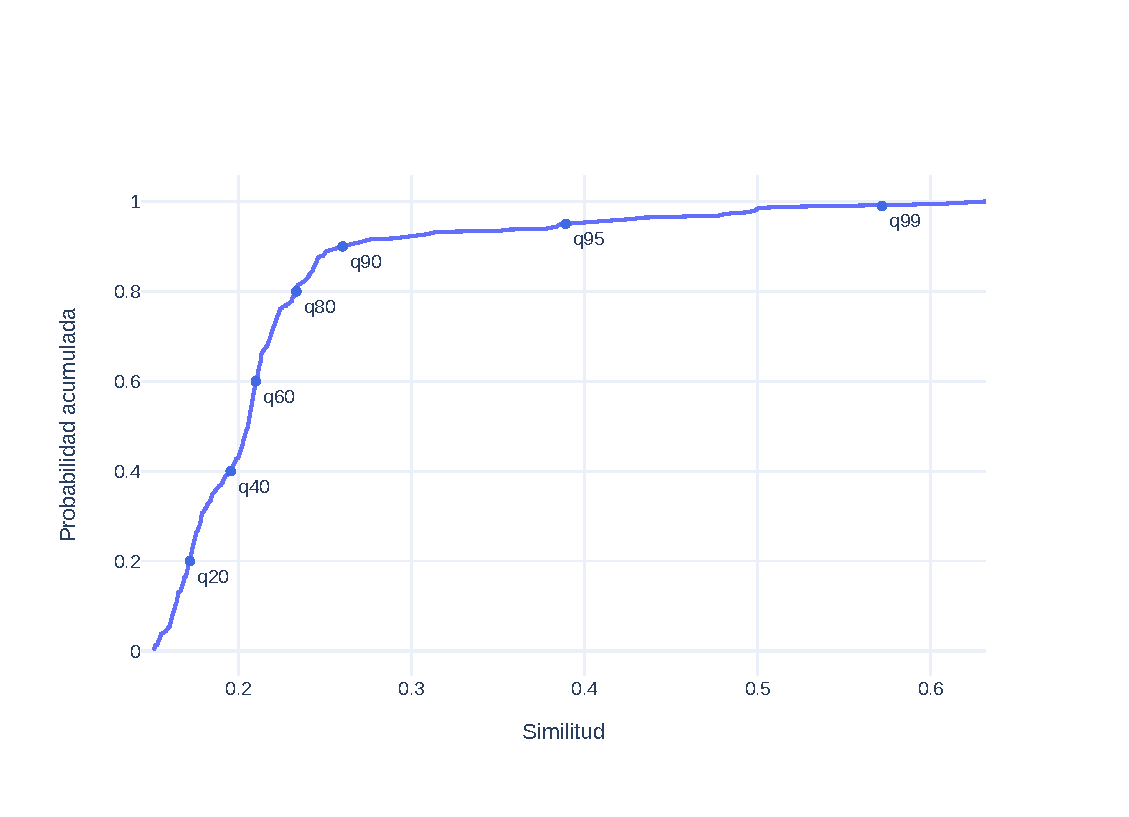
\includegraphics[width=\textwidth]{ch4/cdf.eps}
    \caption{Estimación empírica de la cdf de la similitud WMD entre tópicos del grafo \textit{fully-conected}.}
    \label{img:cdf_wmd}
\end{figure}

En la Figura \ref{img:temporal_similarity_graphs} se muestran los grafos resultantes tras aplicar distintos puntos operantes $\zeta$. Como es esperado, un incremento de $\zeta$ resulta en un incremento en la \textit{sparsity} del grafo temporal.

\begin{figure}
\centering
\subfloat[$\zeta$ = 0]{
  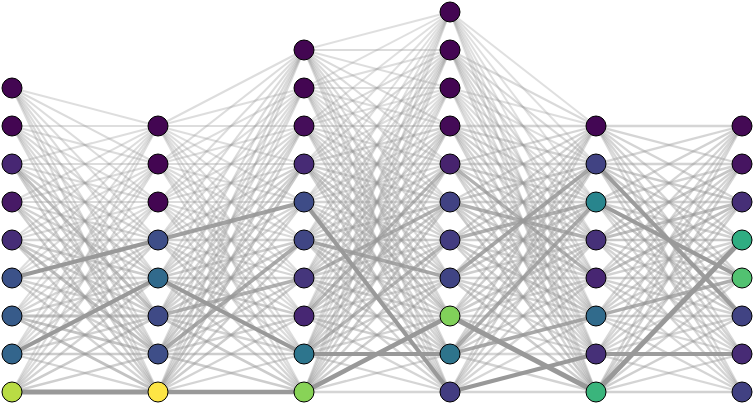
\includegraphics[width=0.4\textwidth]{ch4/graph_q100.png}
}
\subfloat[$\zeta$ = 0.9]{
  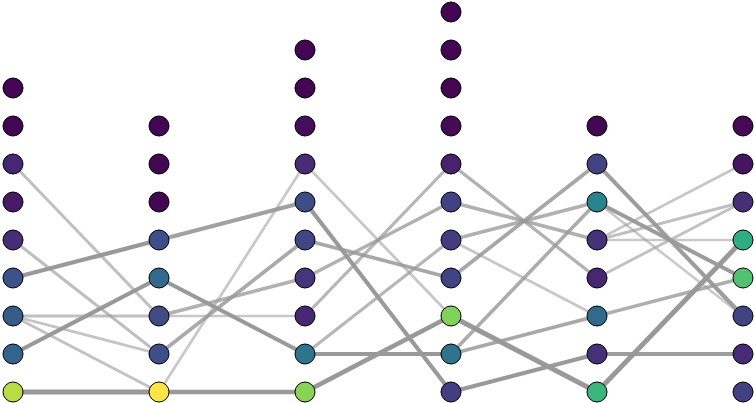
\includegraphics[width=0.4\textwidth]{ch4/graph_q100_e90.png}
}\\
\subfloat[$\zeta$ = 0.95]{
  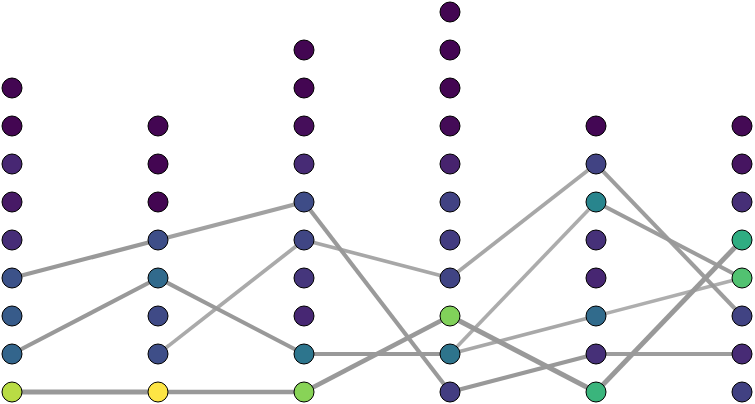
\includegraphics[width=0.4\textwidth]{ch4/graph_q100_e95.png}
}
\subfloat[$\zeta$ = 0.99]{
  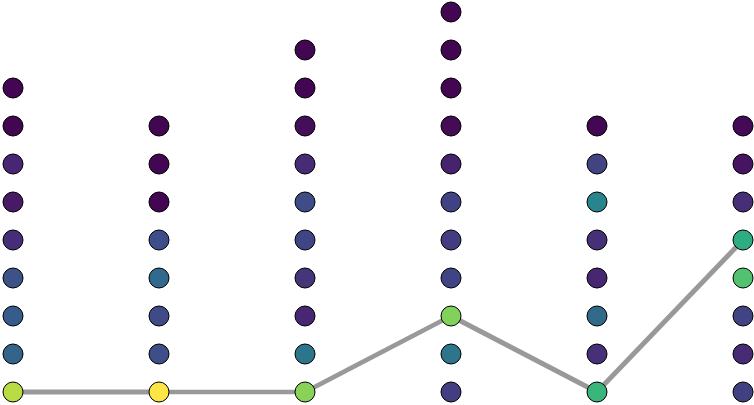
\includegraphics[width=0.4\textwidth]{ch4/graph_q100_e99.png}
}\\
\caption{Grafo de similitud temporal. Los grafos corresponden al mismo corpus y fueron construidos usando el mismo conjunto de tópicos con WMD como medida de similitud, pero bajo diferentes puntos operantes $\zeta$ de la CDF. El eje horizontal denota el tiempo en años, partiendo en el 2011 hasta el 2016, donde cada columna de tópicos corresponde a una época específica. Mientras más claro sea el color del nodo que representa un tópico más popularidad posee en su correspondiente época y mientras mayor es el grosor del arco entre dos tópicos mayor es su similitud.}
\label{img:temporal_similarity_graphs}
\end{figure}

En el grafo podado se pueden identificar diferentes dinamismos en cada época, como nacimiente, muerte, evolución, fusión y división. Un tópico nace en una época si en la época anterior no posee antecesores. La época de muerte de un tópico se identifica como aquella en que no tiene ningún descendiente. Un tópico evoluciona si posee un único antecesor. La fusión ocurre en una época cuando un tópico tiene más de un antecesor. En cambio, la división ocurre cuando hay dos o más tópicos de una época que comparten un antecesor.\\

En la Figura \ref{img:topics_evolution} se muestra la proporción de tópicos que nacen, mueren, fusionan, y dividen por época, normalizando por el número total de tópicos inferido en esa época. Se puede observar que al incrementar $\zeta$ la proporción de tópicos que nacen y mueren aumenta significativamente, puesto que al ser mayor el úmbral de corte menos ascendentes y descendientes se tienen, por otro lado, la división y fusión decrecen, debido a la menor presencia de conexiones.

\begin{figure}
    \centering
    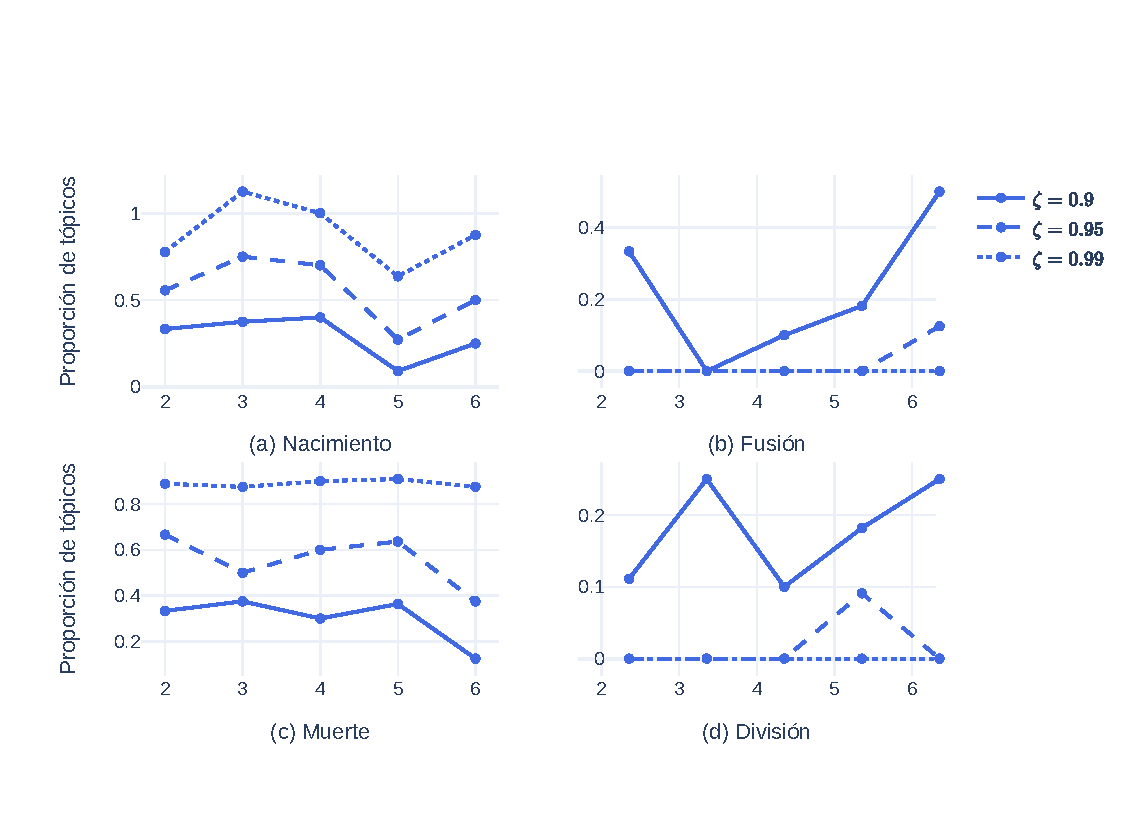
\includegraphics[width=\textwidth]{ch4/topics_evolution.eps}
    \caption{Proporción de tópicos que nacen, mueren, fusionan y dividen por época, normalizando por el número total de tópicos inferido en esa época, bajo diferentes puntos operantes $\zeta$.}
    \label{img:topics_evolution}
\end{figure}

\subsection{Heurística de mejora del tiempo de construcción del grafo de similitud}

WMD es una medida intensiva en recursos computacionales, por lo que se requiere de heurísticas para escalar la metodología a un gran volumen de datos. Como se menciona en la sección \ref{sec:wmd_complexity} una forma de reducir significativamente el tiempo de creación del grafo temporal es utilzar el top N de palabras más probables del tópico que expliquen determinado porcentaje de la distribución acumulada. A la hora de aplicar esta heurística se debe tener en cuenta la posible pérdida de información al representar un tópico con un vocabulario reducido. Sea $G_{\zeta}$ el grafo obtenido al aplicar tras podar el grafo completo con un punto operante $\zeta$ y $G^{'}_{\zeta}$ el grafo aproximado de aplicar la heurística, con $E$ y $E^{'}$ los conjuntos de arcos respectivos. Luego, el porcentaje de arcos correctos de la heurística corresponde a la cardinalidad de la intersección divida por la cardinalidad de la unión, matemáticamente:

\begin{equation}
  \frac{|E\cap E^{'}|}{|E\cup E^{'}|}
\end{equation}

En la Figura \ref{img:speedup} se muestra la mejora en \textit{speedup} y el incremento en error al usar un porcentaje menor de la cdf del tópico para construir el grafo de similitud temporal. Utilizando el 20\% de la cdf la construcción del grafo de similitud disminuye en más de 1,207 veces, esto bajo un error medianamente aceptable del orden del 10-30\%. Si se utiliza un 60\% de la cdf el tiempo mejora en casi 137 veces, siendo el error menor al 10\%. Por otro lado, si se utiliza un 90\% de la cdf el error es inferior al 5\%, siendo el speedup es aproximadamente 8 veces superior a utilizar el vocabulario completo del tópico en la construcción del grafo temporal.

\begin{figure}
    \centering
    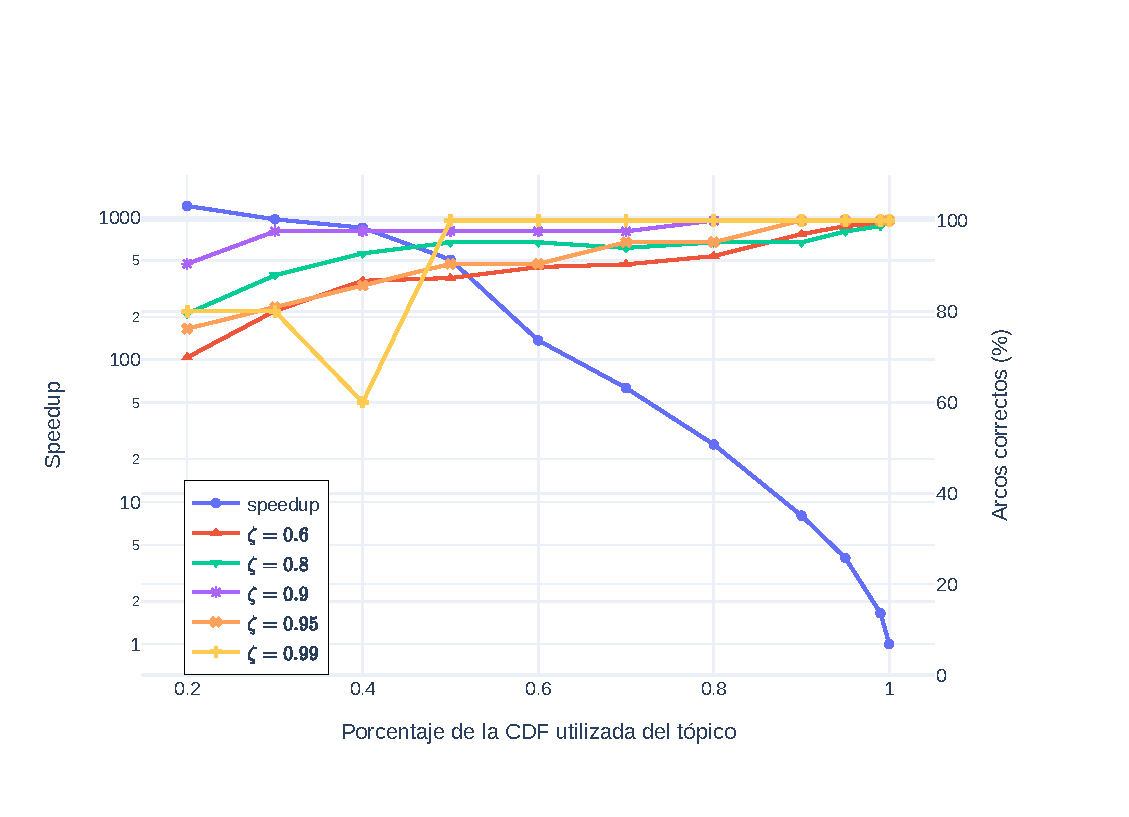
\includegraphics[width=\textwidth]{ch4/speedup.eps}
    \caption{\textit{Speedup} y porcentaje de arcos correctos al utilizar un menor porcentaje de la cdf de los tópicos en la construcción del grafo de similitud. El error de la heurística es mostrado para diferentes puntos operantes $\zeta$ utilizados para podar el grafo completo.} 
    \label{img:speedup}
\end{figure}

\section{Análisis cualitativo de resultados}
\label{sec:qualitative}

En esta sección se realiza un análisis cualitativo de los tópicos descubiertos y su evolución. El análisis es realizado sobre el grafo podado con un punto operante $\zeta = 0.95$ mostrado en la Figura \ref{img:temporal_similarity_graphs}. En las siguientes dos subsecciones se analizan los dos tópicos más predominantes en el tiempo: en la sección \ref{sec:noviolence_topic} se estudia el robo no presencial y en la sección \ref{sec:violence_topic} se analiza el robo con violencia.

\subsection{Evolución del robo no presencial}
\label{sec:noviolence_topic}

En la Figura \ref{img:noviolence_topic} se muestra la evolución de uno de los tópicos más predominantes del grafo temporal. A diferencia de otros tópicos este tópico no presenta en el tiempo división, fusión ni desaparición. En base a las top 10 palabras más probables el tópico se puede caracterizar como un robo bajo las siguientes circunstancias: vehículo estacionado en la calle, sin la presencia del conductor, el conductor al regresar al lugar se percata de la ausencia del vehículo. Un nombre adecuado para este tópico podría ser \quotes{robo no presencial}, ya que se caracteriza por no contar con la presencia del conductor cuando ocurre el robo. Este tópico se caracteriza por su gran estabilidad en el tiempo, ya que en el top 10 se encuentran practicamente las mismas palabras. Por último, se observa una tendencia a la baja de la participación del tópico, en el año 2011 alrededor del 44\% de los \textit{tokens} provienen de este tópico y en el año 2016 se tiene un 32\%.

\def\topic[#1,#2,#3,#4,#5,#6]#7{
        \node[fill=#1, rounded corners, minimum height=#2, minimum width=#3, text width=4em] (#5) at #6 {}; 
        \node[anchor=#4,inner sep=2pt,] at (#5.#4)  {#7};
}
\def\tedge[#1,#2,#3,#4,#5];{ 
  \definecolor{color0}{RGB}{153,153,153}
  \draw[color=color0,#4,fill=white, line width=4*#5pt] (#1) -- #3
  (#2);  
}

\definecolor{color1}{RGB}{184,222,41}
\definecolor{color2}{RGB}{253,231,37}
\definecolor{color3}{RGB}{134,213,73}
\definecolor{color4}{RGB}{127,211,78}
\definecolor{color5}{RGB}{52,182,121}
\definecolor{color6}{RGB}{40,174,128}

\begin{figure}
\begin{tikzpicture}
  \topic[color1,60,80,north,t1,(0,0)] {
     \scriptsize
     \begin{tabular}{l}
       estacionado deje\\
       calle encontraba\\
       lugar regresar\\
       domicilio volver\\
       percato salir
     \end{tabular}
  }
  \topic[color2,60,80,north,t2,(3,0)] {
     \scriptsize
     \begin{tabular}{l}
       estacionado deje\\
       calle lugar\\
       encontraba domicilio\\
       percato salir\\
       volver regresar
     \end{tabular}
  };
  \topic[color3,60,80,north,t3,(6,0)] {
     \scriptsize
     \begin{tabular}{l}
       estacionado deje\\
       calle encontraba\\
       lugar percato\\
       domicilio frente\\
       regresar salir
     \end{tabular}
  };
  \topic[color4,60,80,north,t4,(9,0)] {
     \scriptsize
     \begin{tabular}{l}
       estacionado deje\\
       calle lugar\\
       encontraba domicilio\\
       percato volver\\
       dejo salir
     \end{tabular}
  };
  \topic[color5,60,80,north,t5,(12,0)] {
     \scriptsize
     \begin{tabular}{l}
       estacionado deje\\
       calle lugar\\
       encontraba percato\\
       domicilio volver\\
       salir dejo
     \end{tabular}
  };
  \topic[color6,60,80,north,t6,(15,0)] {
     \scriptsize
     \begin{tabular}{l}
       estacionado deje\\
       calle lugar\\
       econtraba percato\\
       salir camioneta\\
       dejo domicilio
     \end{tabular}
  };
  \tedge[t1,t2,,,0.625];
  \tedge[t2,t3,,,0.586];
  \tedge[t3,t4,,,0.581];
  \tedge[t4,t5,,,0.632];
  \tedge[t5,t6,,,0.609];
\end{tikzpicture}
\caption{Evolución del tópico de robo de vehículo no presecial. El eje horizontal denota el tiempo en años, partiendo en el 2011 hasta el 2016. Mientras más claro el color del tópico más popularidad posee en su correspondiente época y mientras mayor es el grosor del arco entre dos tópicos mayor es su similitud.}
\label{img:noviolence_topic}
\end{figure}

\subsection{Evolución del robo con violenca}
\label{sec:violence_topic}

En la Figura \ref{img:violence_topic} se describe un tipo de robo de vehículo que se puede clasificar como robo con violencia. Este delito, se presenta de la siguiente forma: un conjunto de personas se bajan de un vehículo, intimidan al conductor mediante una pistola u otra arma de fuego, le quitan las llaves del vehículo y finalmente se llevan el vehículo dándose a la fuga. La participación de este tipo de robo se ha visto al alza, en el 2011 su participación era del 12\% y en el 2016 del 36\%, por lo que se ha convertido en un delito más a la moda, quitandole terreno al robo no presencial. A diferencia del tópico robo no presencial este presenta una fusión y división en el 2015. En ese año emerge del robo con violencia un subtópico popularmente conocido como \quotes{portonazo}, un robo con violencia que se caracteriza por la sustracción del vehículo en el portón de la casa de la víctima. Ese año coincide con la popularización de aquel \textit{modus operandi}. Al siguiente año el subtópico se vuelve a fusionar para formar parte del tópico robo con violencia de períodos anteriores.

\definecolor{color1}{RGB}{50,100,142}
\definecolor{color2}{RGB}{48,105,142}
\definecolor{color3}{RGB}{43,116,142}
\definecolor{color4}{RGB}{44,115,142}
\definecolor{color51}{RGB}{37,133,142}
\definecolor{color52}{RGB}{48,106,142}
\definecolor{color6}{RGB}{78,195,107}

\begin{figure}
\begin{tikzpicture}
  \topic[color1,60,80,north,t1,(0,0)] {
     \scriptsize
     \begin{tabular}{l}
       arma personas\\
       tipos individuos\\
       llaves fuego\\
       calle pistola\\
       llevaron bajar
     \end{tabular}
  }
  \topic[color2,60,80,north,t2,(3,0)] {
     \scriptsize
     \begin{tabular}{l}
       llaves personas\\
       individuos tipos\\
       calle persona\\
       arma pistola\\
       bajar llevaron
     \end{tabular}
  };
  \topic[color3,60,80,north,t3,(6,0)] {
     \scriptsize
     \begin{tabular}{l}
       personas calle\\
       llaves individuos\\
       arma pistola\\
       fuego tipos\\
       llevaron fuga
     \end{tabular}
  };
  \topic[color4,60,80,north,t4,(9,0)] {
     \scriptsize
     \begin{tabular}{l}
       personas individuos\\
       tipos calle\\
       llaves arma\\
       llevaron sujetos\\
       fuego armas
     \end{tabular}
  };
  \topic[color51,60,80,north,t51,(12,1.2)] {
     \scriptsize
     \begin{tabular}{l}
       bajan individuos\\
       llaves armas\\
       algun calle\\
       fuego personas\\
       sujetos todas
     \end{tabular}
  };
  \topic[color52,60,80,north,t52,(12,-1.2)] {
     \scriptsize
     \begin{tabular}{l}
       llaves tipos\\
       pitola personas\\
       casa llevaron\\
       bajaron arma\\
       porton puerta
     \end{tabular}
  };
  \topic[color6,60,80,north,t6,(15,0)] {
     \scriptsize
     \begin{tabular}{l}
       personas bajan\\
       calle arma\\
       tipos llaves\\
       fuego individuos\\
       armas pistola
     \end{tabular}
  };
  \tedge[t1,t2,,,0.499];
  \tedge[t2,t3,,,0.498];
  \tedge[t3,t4,,,0.5];
  \tedge[t4,t51,,,0.422];
  \tedge[t4,t52,,,0.405];
  \tedge[t51,t6,,,0.395];
  \tedge[t52,t6,,,0.483];
\end{tikzpicture}
\caption{Evolución del tópico de robo con violencia de vehículo. El eje horizontal denota el tiempo en años, partiendo en el 2011 hasta el 2016. Mientras más claro el color del tópico más popularidad posee en su correspondiente época y mientras mayor es el grosor del arco entre dos tópicos mayor es su similitud.}
\label{img:violence_topic}
\end{figure}


\chapter{Conclusiones y trabajo futuro}
\label{ch:conclusion}
Este trabajo se enfoca en el modelamiento y descubrimiento de tópicos en el tiempo en un corpus. El enfoque descrito comienza con la discretización del corpus en épocas. Luego, usando como aproximación que la estructura de los tópicos dentro de cada época es estática, los tópicos son descubiertos usando Hierarchical Dirichlet Process. Por último, la evolución de los tópicos en el tiempo es modelada por un grafo temporal sustentado por una medida de similitud entre tópicos. El grafo inicialmente es construido por los arcos entre todos los pares de tópicos de épocas adyacentes, luego es podado automáticamente en base a un punto operante de la cdf de la similitud. Esta estructura permite inferir cambios estructurales complejos de los tópicos, como nacimiento, muerte, división, fusión y evolución en el tiempo.\\

En contraste a trabajos anteriores, la metodología propuesta utiliza Word Mover's Distance como medida de similitud entre tópicos, permitiendo comparar de forma más apropiada tópicos que no poseen un vocabulario común a través de sus \textit{word embeddings}. Además, se presenta una análisis empírico del \textit{trade off} entre precisión y \textit{speedup} de no utilizar el vocabulario completo del tópico en la construcción del grafo de similitud.\\

Resultados experimentales al fenómeno de robo de vehículos son reportados. Se muestra el efecto que tiene la elección del punto operante de la cdf en la construcción del grafo final. Otro importante hallazgo, es el nivel de consistencia de la metodología en modelar de la evolución de los tópicos en el tiempo, siendo capaz de relacionar tópicos que evidentemente son similares, como es el caso del robo no presencial o el robo con violencia.\\

La metodología propuesta puede tener otros usos interesantes como descubrir nuevas tendencias de investigación, analizar la evolución de la contigencia social, estudiar la efectividad de campañas publicitarias en base a la opinión de los consumidores, organizar y recomendar contenido en un blog, etc.\\

Como trabajo futuro podría ser interesante extender la metodología a un enfoque puramente basado en redes neuronales. De esta forma la comparación entre tópicos de épocas adyacentes a través de sus \textit{word embeddings} se vuelve más natural. También sería más consistente ya que la información codifica en los \textit{word embeddings} se utilizaría para el mismo descubrimiento de los tópicos. En \cite{dieng2019dynamic} se propone una modelo de tópicos dinámico basado en redes neuronales, no obstante, mantiene fijo el número de tópicos en el tiempo.


\bibliography{main}

% FIN DEL DOCUMENTO
\end{document}